\documentclass{book}
%\usepackage[spanish]{babel}
\RequirePackage{etex}
\usepackage[utf8]{inputenc}
\usepackage{braket}
%\usepackage[sc]{mathpazo}
% \linespread{1.5}
%\usepackage[T1]{fontenc}
%\usepackage{heuristica}
%\usepackage[erewhon,vvarbb,bigdelims]{newtxmath}
%\renewcommand*\oldstylenums[1]{\textosf{#1}}
\usepackage{enumitem}
\usepackage{array}
\usepackage{textcomp}
\usepackage{fancyhdr}
\usepackage{amsmath, amsthm}
\usepackage{slashed}
\usepackage[normalem]{ulem}
\usepackage{amsfonts}
\usepackage{amssymb}
\usepackage{mathtools}
\usepackage{float}
\usepackage{soul}
\usepackage{graphicx}
\usepackage{hyperref}
\usepackage{graphicx}
\usepackage{pstricks-add}
\usepackage{color}
\usepackage{caption}
\usepackage[margin=0.9in]{geometry}
\usepackage{marvosym}
\usepackage{mathtools}
\usepackage{framed}
\usepackage{calrsfs}
\usepackage[mathscr]{euscript}
\usepackage{tensor}
\usepackage{autonum}
\usepackage{cancel}
\usepackage[most]{tcolorbox}
\usepackage{multicol}
\usepackage{tikz}
\usepackage{pdfpages}


\newcommand{\brackets}[1]{\left[#1\right]}
\newcommand{\curlybraces}[1]{\left\{#1\right\}}
\newcommand{\qedh}{\hfill\hspace{5mm}\fbox{\phantom{\rule{.5ex}{.5ex}}}}

\newenvironment{Figura}
  {\par\medskip\noindent\minipage{\linewidth}}
  {\endminipage\par\medskip}
\newtheorem{thm}{Teorema}[section]
\newtheorem{theorem}{Teorema}[section]
\newtheorem{proposition}[thm]{Proposición} 
\newtheorem{lemma}[thm]{Lema}
\newtheorem{corollary}[thm]{Corolario} 
\newtheorem{conv}[thm]{Convención}
\newtheorem{defi}[thm]{Definición}
\newtheorem{definition}[theorem]{Definición}
\newtheorem{notation}[thm]{Notación} 
\newtheorem{exe}[thm]{Ejemplo}
\newtheorem{conjecture}[thm]{Conjetura} 
\newtheorem{prob}[thm]{Problema}
\newtheorem{remark}[thm]{Observación}
\newtheorem{example}[thm]{Ejemplo}
\newtheorem{note}[thm]{Nota}
\newcommand{\abss}[1]{\left|#1\right|^2}
\newcommand{\scalar}[2]{\langle #1, #2 \rangle}
\newcommand{\ptensor}[2]{#1 \otimes #2}
\newcommand{\pcart}[2]{#1 \times #2}
\newcommand{\vvector}[3]{\begin{pmatrix}#1\\ #2\\ #3\end{pmatrix}}
\newcommand{\covector}[3]{\begin{pmatrix}#1 & #2 & #3\end{pmatrix}}
\newcommand{\dket}[2]{\begin{matrix}#1 & #2 \end{matrix}}
\newcommand{\ddket}[3]{\begin{matrix} #1 & #2 & #3 \end{matrix}}
\newcommand{\voverrightarrowtor}[3]{\begin{pmatrix}#1\\ #2\\ #3\end{pmatrix}}
\newcommand{\cooverrightarrowtor}[3]{\begin{pmatrix}#1 & #2 & #3\end{pmatrix}}


\begin{document}
\pagestyle{empty}
\begin{titlepage} 

	\newcommand{\HRule}{\rule{\linewidth}{0.5mm}} 
	
	\center 
	\textsc{\LARGE Facultad de Ciencias}\\[1.5cm] 
	
	\textsc{\Large Grado de Física}\\[0.5cm] 
	\textsc{\large Mecánica Cuántica}\\[0.5cm] 
	
	\HRule\\[0.4cm]
	
	\huge\bfseries Temario Mecánica Cuántica 24-25 \\[0.3cm] 
	\HRule\\[1cm]
	
	\vfill
	\includegraphics[width=10cm]{UGR-MARCA-01-color.png} 
	\vfill \vfill \vfill
	\begin{minipage}{0.7\textwidth}
		\begin{flushleft}
		\Large
			\textit{Autor}\\
			Rubén Carrión Castro\\
			
		\end{flushleft}
	\end{minipage}
	
	
	\vfill\vfill\vfill % Position the date 3/4 down the remaining page
	

	\vfill 
	
\end{titlepage}

\tableofcontents
\listoffigures
 
\setcounter{page}{1}
\pagestyle{fancy}
\chapter{Postulados de la Mecánica Cuántica }
\section{Introducción: Experimento de Stern-Gerlach}
El experimento de Stern y Gerlach, nombrado así en honor de los físicos alemanes Otto Stern y Walther Gerlach, es un famoso experimento realizado por primera vez en 1922 sobre la deflexión de partículas y que ayudó a sentar las bases experimentales de la mecánica cuántica. Puede utilizarse para ilustrar que los electrones y átomos tienen propiedades cuánticas intrínsecas, que las medidas afectan a las propiedades de las partículas medidas y que los estados cuánticos necesariamente se describen a través de números complejos.\\ \\
Este experimento pretende medir el momento magnético de un átomo de plata. El dispositivo es el mostrado en la Figura \ref{fig1}.

\begin{Figura}
    \centering
    \includegraphics[width=1\textwidth]{image.png}
    \captionof{figure}{Esquema del experimento de Stern-Gerlach}
    \label{fig1}
\end{Figura}

Un átomo visto de forma clásica tiene un momento angular $\Vec{L}=\vec{r}\times\vec{p}$ y un momento magnético $\vec{\mu}=\frac{q}{2m}\vec{L}$. Así, el experimento de Stern-Gerlach usa un campo magnético uniforme que tiende a alinear los momentos magnéticos de los átomos.\\ \\
Un átomo visto de forma cuántica son orbitales con momento angular orbital $\vec{L}$, el cuál interacciona con $\vec{B}$ de la misma manera que el momento magnético, pues $\vec{\mu}=\frac{q}{2m}\vec{L}$; además, hay un momento angular de espín $\vec{S}$ que también interacciona con $\vec{B}$, tal que $\vec{\mu}=g\frac{q}{2m}\vec{S}$, con $g=2$, que se demuestra con la Mecánica Cuántica relativista de Dirac. Además, usando Teoría Cuántica de Campos, podemos obtener un valor teórico muy preciso de $g$, pues $g_{teor}-2=0,0023193043632\pm15$ y $g_{exp}-2=0,0023193043611\pm20$.\\ \\
Como los átomos de plata tienen 47 electrones, el momento de espín, o magnético, que queremos medir es el del electrón 47. Cuando $\vec{\mu}$ atraviesa $\vec{B}$, experimenta una fuerza, que viene dada por el potencial,
\[E_p=-\vec{\mu}\cdot\vec{B}\overset{\curlybraces{\vec{B}=(0,0,B(z))}}{=}-\mu_zB(z)\]
y así, la fuerza queda,
\[\vec{F}=-\vec{\nabla}E_p=-\frac{\partial}{\partial z}(-\mu_zB(z))=\mu_z\frac{\partial B(z)}{\partial z}\]
Así, viendo cómo se desvía el átomo, conocemos $\mu_z$ y por tanto, conocemos $S_z$. Es decir, la deflexión (lo que se desvía) del átomo de plata es una medida de $S_z$.
\begin{multicols}{2}
    \begin{Figura}
        \centering
        \includegraphics[width=1\textwidth]{a.png}
        \captionof{figure}{Resultado esperado.}
        \label{fig2}
    \end{Figura}
    \begin{Figura}
        \centering
        \includegraphics[width=1\textwidth]{b.png}
        \captionof{figure}{Resultado experimental.}
        \label{fig3}
    \end{Figura}
\end{multicols}

Como vemos en las figuras \ref{fig2} y \ref{fig3}, los resultados esperados no son lo resultados experimentales.\\ \\
-La primera conclusión que obtenemos es que los posibles valores de la componente $z$ del momento angular de espín del átomo de plata están cuantizados, es decir, no son un continuo de valores, pues tenemos $S_z=\pm\frac{\hbar}{2}$; obteniendo el mismo resultado para $S_x$ y $S_y$.\\ \\
Planteamos ahora un Stern-Gerlach secuencial, de forma que un Stern-Gerlach del eje Z, emita dos haces, un 50$\%$ con $S_z^+$ y el otro 50$\%$ con $S_z^-$. Ahora ponemos un Stern-Gerlach del eje X en el haz de 50$\%$ de $S_z^+$, haciendo que emita otra vez 50 y 50. Colocamos un tercer Stern-Gerlach, del cuál esperamos que emita un solo haz con un 100$\%$ de $S_z^+$, pero no ocurre esto, sino que se vuelven a emitir dos haces con 50-50, cosa que es imposible de explicar con la mecánica clásica.\\ \\
-La segunda conclusión que obtenemos es que es imposibles preparar un átomo de $Ag$ (o de cualquier sistema) con un valor bien definido de $S_z$ y $S_x$, porque la medida de $S_x$ cambia el valor de $S_z$.\\ \\
-La tercera conclusión que sacamos en que importa el orden temporal en el que hacemos las medidas.
\section{Estados 'bras' y 'kets'}
\begin{tcolorbox}[title=Postulado 1]
    En mecánica cuántica, el estado $\alpha$ de un sistema físico, a un tiempo $t$, se describe mediante un vector unitario de un cierto espacio de Hilbert complejo. El vector, que describe el estado de mi sistema, se denomina vector estado (o estado) o 'ket' (en notación de Dirac), y se denota por $\ket{\alpha}$ ó $\ket{\alpha(t)}$.
\end{tcolorbox}
El espacio de Hilbert $\mathscr{H}$ es un espacio vectorial normado cuyos vectores pueden:
\begin{itemize}
    \item combinaciones lineales.
    \item multiplicar por números complejos.
    \item $\vec{v}\to\ket{v}$ (cambio de notación)
    \item Si $\ket{\alpha},\ket{\beta}\in\mathscr{H}$ y $a,b\in\mathbb{C}$, entonces $a\ket{\alpha}+b\ket{\beta}\in\mathscr{H}$.
    \item Existe el vector nulo, $0\ket{\alpha}=0\neq\ket{0}$, pues $\ket{0}$ es el vacío.
\end{itemize}
\subsection{Base ortonormal}
Una base es un conjunto de vectores linealmente independientes, $B=\curlybraces{\ket{e_i};i=1,\dots,n}$, tal que $\ket{\alpha}\in\mathscr{H}$ puede escribirse como,
\[\begin{array}{rl}
    \ket{\alpha} & =\ket{e_1}\alpha^1+\ket{e_2}\alpha^2+\dots\ket{e_n}\alpha^n= \\
     & =\sum\limits_i\ket{e_i}\alpha^i\equiv\ket{e_i}\alpha^i=\\
     & = \begin{pmatrix}
         \ket{e_1} & \ket{e_2} & \dots & \ket{e_n}
         \end{pmatrix}
         \begin{pmatrix}
             \alpha^1\\
             \alpha^2\\
             \vdots\\
             \alpha^n
     \end{pmatrix}
\end{array}\]
donde podemos identificar el vector $\ket{\alpha}$ por sus componentes de la base, tal que
\[\ket{\alpha}\doteq\begin{pmatrix}
    \alpha^1\\
    \alpha^2\\
    \vdots\\
    \alpha^n
\end{pmatrix}\]
donde los $\alpha^i$ son las componentes contravariantes de $\ket{\alpha}$ en la base $\curlybraces{\ket{e_i}}$.\\ \\
La ortonormalidad de una base puede definirse usando el producto escalar o usando un isomorfismo con el espacio dual $\mathscr{H}^*$.
\subsubsection{Producto escala}
Dados dos vectores $\ket{\alpha},\ket{\beta}\in\mathscr{H}$, el \textit{producto escalar de }$\ket{\alpha}$\textit{ por }$\ket{\beta}$ se escribe como $\braket{\alpha|\beta}\in\mathbb{C}$, que cumple las condiciones del producto escalar:
\begin{itemize}
    \item linealidad,
    \[\bra{\alpha}(a_1\ket{\beta_1}+a_2\ket{\beta_2})=a_1\braket{\alpha|\beta_1}+a_2\braket{\alpha|\beta_2}\]
    \item el resto de condiciones
    \item Hermiticidad,
    \[\braket{\beta|\alpha}=\braket{\alpha|\beta}^*\]
\end{itemize}
El producto escalar define el módulo del vector $\ket{\alpha}$, tal que $\left|\ket{\alpha}\right|=\sqrt{\braket{\alpha|\alpha}}$, y la distancia entre dos vectores, tal que $d\left(\ket{\alpha},\ket{\beta}\right)=\left|\ket{\alpha}-\ket{\beta}\right|$.\\ \\
Una vez obtenido el producto escalar, podemos hacer el producto escalar entre vectores de la base, el cuál define la \textbf{métrica}, así $\braket{e_i|e_j}=g_{ij}$. Diremos que la base $\curlybraces{\ket{e_i}}$ es ortonormal si $\braket{e_i|e_j}=\delta_{ij}$, donde $\delta_{ij}$ es la delta de Kronecker, y que $|\ket{e_i}|=1$.
\subsubsection{Isomorfo con el espacio dual $\mathscr{H}^*$}
Un formalismo equivalente (el usual en mecánica cuántica), es el basado en 'bras' y 'kets'.\\ \\
Dado un espacio de Hilbert $\mathscr{H}$, de vectores o 'kets' $\ket{\alpha}\in\mathscr{H}$, definimos su espacio dual $\mathscr{H}^*$, de covectores o 'bras' $\bra{\beta}\in\mathscr{H}^*$, como el conjunto de todas las formas lineales que asignan un número complejo a cada vector de $\mathscr{H}$. Así, una forma lineal será
\[\begin{array}{rcl}
    \bra{\beta}:\ket{\alpha} & \to & \braket{\beta|\alpha}\in\mathbb{C}
\end{array}\]
donde $\bra{\beta}\in\mathscr{H}^*$, $\ket{\alpha}\in\mathscr{H}$ y $\braket{\beta|\alpha}$ se denomina 'braket'.\\ \\
Puede mostrarse que $\mathscr{H}$ y $\mathscr{H}^*$ son isomorfos, en particular, tienen la misma dimensión. Entonces, establecer un isomorfismo entre $\mathscr{H}$ y $\mathscr{H}^*$ es equivalente a definir una métrica (un producto escalar):
\[\begin{array}{rcl}
    \mathscr{H} & \overset{\dagger}{\longleftrightarrow} & \mathscr{H}^* \\
    \ket{\alpha} & \overset{\dagger}{\longleftrightarrow} & \bra{\alpha}\equiv\ket{\alpha}^{\dagger}
\end{array}\]
donde $\dagger$ se denomina \textbf{adjunto}. Es una relación antilineal, es decir, $(a\ket{\alpha})^{\dagger}=a^*\bra{\alpha}$, con $a\in\mathbb{C}$. En particular, a una base de $\mathscr{H}$, $\curlybraces{\ket{e_i}}$, denominamos base adjunta,
\[\curlybraces{\ket{e_i}}\to\curlybraces{\bra{e_i}}\]
tal que $\braket{e_i|e_j}=g_{ij}\in\mathbb{C}$, que vemos que es equivalente al producto escalar definido anteriormente. Así, $\braket{e_i|e_j}$ se denomina el producto escalar de $\ket{e_i}$ por $\ket{e_j}$ o la acción de $\bra{e_i}$ sobre $\ket{e_j}$.\\ \\
Decimos que $\curlybraces{\ket{e_i}}$ es una base ortonormal de $\mathscr{H}$, y $\curlybraces{\bra{e_i}}$ es una base ortonormal de $\mathscr{H}^*$ si $\braket{e_i|e_j}=\delta_{ij}$.\\ \\
Hemos visto que $\ket{\alpha}=\ket{e_i}\alpha^i$, donde las $\alpha^i$ son las \textit{componentes contravariantes} de $\ket{\alpha}$.\\ \\
Consideraremos un \textbf{cambio de base}, $\curlybraces{\ket{e_i}}\to\curlybraces{\ket{\tilde{e}_i}}$, es decir,
\[\ket{\tilde{e}_i}=\ket{e_j}A_i^j\equiv\left(\sum_j\ket{e_j}A_i^j=\ket{e_1}A_i^1+\ket{e_2}A^2_i+\dots\right)\]
con $A_i^j\in\mathbb{C}$, $i,j=1,2\dots,n$. Así tenemos un sistema de $n-$ecuaciones que podemos reescribir en forma matricial tal que
\[\begin{pmatrix}
    \ket{\tilde{e}_1} & \ket{\tilde{e}_2} & \dots
\end{pmatrix}=\begin{pmatrix}
    \ket{e_1} & \ket{e_2} & \dots
\end{pmatrix}\begin{pmatrix}
    A_1^1 & A_2^1 & \dots \\
    A_2^1 & A_2^2 & \dots \\
    \vdots & \vdots & \ddots
\end{pmatrix}\]
donde $A$ es la matriz de cambio de base.\\ \\
Vemos ahora cómo se relacionan las componentes de $\ket{\alpha}$ en ambas bases:
\[\ket{\alpha}=\ket{e_i}\alpha^i=\ket{\tilde{e}_j}\tilde{\alpha}^j=\ket{e_i}A^i_j\tilde{\alpha}^j\]
Por tanto,
\begin{equation}
    \alpha^i=A_j^i\tilde{\alpha}^j; \hspace{5mm}\tilde{\alpha}^i=(A^{-1})^i_j\alpha^j
\end{equation}
que en forma matricial queda
\[\begin{pmatrix}
    \alpha^1 & \alpha^2 & \dots
\end{pmatrix}=\begin{pmatrix}
    A_1^1 & A_2^1 & \dots\\
    A_2^1 & A_2^2 & \dots\\
    \vdots & \vdots & \ddots
\end{pmatrix}\begin{pmatrix}
    \tilde{\alpha}^1\\
    \tilde{\alpha}^2\\
    \vdots
\end{pmatrix};\hspace{5mm}\begin{pmatrix}
    \tilde{\alpha}^1\\
    \tilde{\alpha}^2\\
    \vdots
\end{pmatrix}=\begin{pmatrix}
    (A^{-1})_1^1 & (A^{-1})_2^1 & \dots\\
    (A^{-1})_2^1 & (A^{-1})_2^2 & \dots\\
    \vdots & \vdots & \ddots
\end{pmatrix}\begin{pmatrix}
    \alpha^1 & \alpha^2 & \dots
\end{pmatrix}\]
donde $A^{-1}$ es la matriz inversa del cambio de base.\\ \\
En $\mathscr{H}^*$, $\curlybraces{\bra{e_i}}$ es la \textit{base adjunta}, pero podemos también definir la \textit{base canónica} $\curlybraces{\bra{e^i}}$. La base adjunta verifica que $\braket{e_i|e_j}=g_{ij}$, mientras que la base canónica verifica que $\braket{e^i|e_j}=\delta_j^i$. La relación entre ambas bases es, $\bra{e_i}=g_{ij}\bra{e^j}$. En la base canónica, el adjunto de $\ket{\alpha}$ es
\[\ket{\alpha}^{\dagger}=\bra{\alpha}=\alpha_i\bra{e^i}\]
donde $\alpha^i$ son las \textit{componentes covariantes} de $\ket{\alpha}$. Como la relación adjunta es antilineal, se verifica que
\[(a\ket{\alpha}+b\ket{\beta})^{\dagger}=a^*\bra{\alpha}+b^*\bra{\beta}\]
y si $\ket{\alpha}=\ket{e_i}\alpha^i$, entonces
\[\bra{\alpha}=\ket{\alpha}^{\dagger}=\alpha^{i*}\bra{e_j}=\alpha^{i*}g_{ij}\bra{e^j}=\alpha_j\bra{e^j}\]
por tanto,
\begin{equation}
    \alpha_i=\alpha^{j*}g_{ij}
\end{equation}
es decir, la métrica sirve para baja índices.\\ \\
\textbf{Nomenclatura}\\ \\
Utilizaremos siempre bases ortonormales y siempre escribiremos todos los índices abajo, es decir, $\ket{\alpha}=\ket{e_i}\alpha_i$, con 
\[\ket{\alpha}\doteq\begin{pmatrix}
    \alpha_1\\
    \alpha_2\\
    \vdots
\end{pmatrix}\]
y $\bra{\alpha}=\alpha_i^*\bra{e_i}$, con
\[\bra{\alpha}\doteq\begin{pmatrix}
    \alpha_1^* & \alpha_2^* & \dots
\end{pmatrix}\]
Recordamos que el Postulado 1 nos decía que un estado físico tiene asociado un cierto vector del espacio de Hilbert, $\ket{\alpha}\in\mathscr{H}$, y que \[\abss{\ket{\alpha}}=1=|\braket{\alpha|\alpha}|=\left|\begin{pmatrix}
    \alpha_1^* & \alpha_2^* & \dots
\end{pmatrix}\begin{pmatrix}
    \alpha_1\\
    \alpha_2\\
    \vdots
\end{pmatrix}\right|=\left|\abss{\alpha_1}+\abss{\alpha_2}+\dots\right|=1\]
\section{Observables}
\begin{tcolorbox}[title=Postulado 2]
    En mecánica cuántica, cada observable físico, $A$, viene representado por un operador lineal hermítico (autoadjunto, es decir, $A^{\dagger}=A$) que actúa sobre el espacio de Hilbert que describe los estados del sistema.
\end{tcolorbox}
Un operador (transformación) lineal $A$ que actúa sobre un espacio vectorial, transforma los vectores del espacio vectorial, $\ket{\alpha}\in\mathscr{H}$, en otro vector $A\ket{\alpha}\in\mathscr{H}$. \\ \\
\textbf{Propiedades:}\\ \\
-Los operadores son lineales, entonces
\[A\left(a\ket{\alpha}+b\ket{\beta}\right)=aA\ket{\alpha}+bA\ket{\beta}\]
-Los operadores pueden sumarse, tal que 
\[(A+B)\ket{\alpha}=A\ket{\alpha}+B\ket{\alpha}\]
-Los operadores pueden multiplicarse, tal que
\[A\cdot B\ket{\alpha}=A(B\ket{\alpha})\]
-Los operadores son transitivos, entonces
\[A\cdot(B\cdot C)=(A\cdot B)\cdot C\]
Para especificar un operador lineal, es suficiente saber cómo actúa sobre la base ortonormal $\curlybraces{\ket{e_i}}$ de $\mathscr{H}$, así
\[\ket{e_i}\overset{A}{\longrightarrow}A\ket{e_i}=\ket{e_i'}=\ket{e_j}A_{ji};\hspace{3mm}A_{ji}\in\mathbb{C}\]
o en forma matricial,
\[\begin{pmatrix}
    \ket{e_1'} & \ket{e_2'} & \dots
\end{pmatrix}=\begin{pmatrix}
    \ket{e_1} & \ket{e_2} & \dots
\end{pmatrix}\begin{pmatrix}
    A_{11} & A_{12} & \dots\\
    A_{21} & A_{22} & \dots\\
    \vdots & \vdots & \ddots
\end{pmatrix}\]
esta es la matriz de la transformación lineal $A$ en la base. Además,
\[\ket{\alpha}\overset{A}{\longrightarrow}\left\lbrace\begin{array}{cl}
    \ket{\alpha'} & =A\ket{\alpha}=A\ket{e_i}\alpha_i=\ket{e_j}A_{ij}\alpha_i \\
    || & \\
    \ket{e_j}\alpha'_j
\end{array}\right.\]
por tanto,
\begin{equation}
    \alpha'_j=A_{ji}\alpha_i
\end{equation}
teniendo $n-$ecuaciones.\\ \\
Entonces, podemos identificar a los operadores lineales por sus matrices en la base, tal que
\[A\doteq\begin{pmatrix}
    A_{11} & A_{12} & \dots\\
    A_{21} & A_{22} & \dots\\
    \vdots & \vdots & \ddots
\end{pmatrix}\]
\subsection{¿Cómo actúa $A$ sobre $\bra{\alpha}\in\mathscr{H}^*$?}
Veamos ahora cómo actúa un operador lineal $A$ sobre un 'bra' del espacio de Hilbert dual, $\bra{\alpha}\in\mathscr{H}^*$. Definimos
\[\begin{array}{cl}
     \bra{e_i}(A\ket{e_j})&\equiv(\bra{e_i}A)\ket{e_i}  \\
    || & \\
    \braket{e_i|e_k}A_{kj}&=\delta_{ik}A_{kj}=A_{ij}
\end{array}\]
Esto implica que
\begin{equation}
    \bra{e_i}A=A_{ij}\bra{e_j}
\end{equation}
Es inmediato demostrar que
\begin{equation}
    \bra{\alpha}A\doteq\begin{pmatrix}
        \alpha_1^* & \alpha_2^* & \dots
    \end{pmatrix}\begin{pmatrix}
        A_{11} & A_{12} & \dots\\
        A_{21} & A_{22} & \dots\\
        \vdots & \vdots & \ddots
    \end{pmatrix}
\end{equation}
Podremos usar representaciones matriciales, tal que
\[\braket{\alpha|A|\beta}=\begin{pmatrix}
    \alpha_1^* & \alpha_2^* & \dots
\end{pmatrix}\begin{pmatrix}
    A_{11} & A_{12} & \dots\\
    A_{21} & A_{22} & \dots\\
    \vdots & \vdots & \ddots
\end{pmatrix}\begin{pmatrix}
    \beta_1\\
    \beta_2\\
    \vdots
\end{pmatrix}\]
\subsubsection{¿Qué es $\ket{\alpha}\bra{\beta}$?}
Es un operador lineal que actúa sobre vectores de $\mathscr{H}$ y devuelve vectores de $\mathscr{H}$, tal que $\ket{\alpha}\braket{\beta|\gamma}$ es un vector en la dirección de $\ket{\alpha}$. Así, en forma matricial tenemos,
\[\ket{\alpha}\bra{\beta}=\begin{pmatrix}
    \alpha_1\\
    \alpha_2\\
    \vdots
\end{pmatrix}\begin{pmatrix}
    \beta_1^* & \beta_2^* & \dots
\end{pmatrix}=\begin{pmatrix}
    \alpha_1\beta_1^* & \alpha_1\beta_2^* & \dots\\
    \alpha_2\beta_1^* & \alpha_2\beta_2^* & \dots\\
    \vdots & \vdots & \ddots
\end{pmatrix}\]
Suponemos que tomamos un vector unitario de la base ortonormal y definimos el operador proyector
\[P_1=\ket{e_1}\bra{e_1}\]
Sobre $\ket{\alpha}=\ket{e_i}\alpha_i$ actuará como,
\[P_1\ket{\alpha}=\ket{e_1}\braket{e_1|e_i}\alpha_i=\ket{e_1}\delta_{1i}\alpha_i=\ket{e_1}\alpha_1\]
así, obtenemos la proyección de $\ket{\alpha}$ sobre la recta generada por el vector $\ket{e_1}$.\\ \\
Este operador es \textbf{idempotente}, es decir, $P_1P_1=P_1$.
\subsubsection{Proyecciones en un espacio tridimensional}
Deberemos usar la suma de dos proyectores, tal que
\[(P_1+P_2)\ket{\alpha}=P_1\ket{\alpha}+P_2\ket{\alpha}=\ket{e_1}\alpha_1+\ket{e_2}\alpha_2\]
pues si usamos un único proyector realmente estamos proyectando en un espacio bidimensional, y si usamos la suma de tres proyecciones, tenemos
\[(P_1+P_2+P_3)\ket{\alpha}=\ket{\alpha}\]
es decir $(P_1+P_2+P_3)=\mathbb{I}$ es el operador identidad. Así, cuando sumamos sobre todos los vectores de la base, tenemos
\[\sum_i\ket{e_i}\bra{e_i}=\mathbb{I}\]
siendo la \textbf{relación de clausura} o de completitud o de cierre.
\\ \\
El adjunto de $A\ket{\alpha}$ viene dado por,
\[(A\ket{\alpha})^{\dagger}=\bra{\alpha}A^{\dagger}\]
El producto escalar de $\ket{\beta}$ por $A\ket{\alpha}$ viene dado por $\braket{\beta|A|\alpha}$; mientras que el producto escalar de $A\ket{\alpha}$ por $\ket{\beta}$ es $\braket{\alpha|A^{\dagger}|\beta}$, denominado \textit{producto escalar adjunto}.\\ \\
Las componentes de $A^{\dagger}$ se pueden obtener como,
\[\left.\begin{array}{cc}
    \braket{e_i|A|e_j} &=A_{ij}  \\
    || & || \\
    \braket{e_j|A^{\dagger}|e_i}^*&=(A^{\dagger}_{ij})^*
\end{array}\right\rbrace\Rightarrow A_{ij}^{\dagger}=A_{ij}^*\Rightarrow A^{\dagger}=A^{\dagger *}\]
\section{Medidas}
\begin{tcolorbox}[title=Postulado 3]
    En la medida de un observable $A$, los únicos valores posibles, de esa medida, son los autovalores, $\curlybraces{a}$, del operador lineal asociado.
\end{tcolorbox}
Los autovalores cumplen que $A\ket{a}=a\ket{a}$, donde $\ket{a}$ es el autovector asociado al autovalor $a$.\\ \\
Si el estado del sistema es $\ket{\alpha}\in\mathscr{H}$, la probabilidad de obtener el autovalor $a$ es:
\begin{enumerate}[label=(\roman*)]
    \item si el autovalor $a$ es no degenerado:
    \[P_a=\abss{\braket{a|\alpha}}=\braket{\alpha|a}\braket{a|\alpha}=\braket{\alpha|P_a|\alpha}=\braket{\alpha|P_a^2|\alpha}=\braket{\alpha|P_aP_a|\alpha}=\abss{P_a\ket{\alpha}}\]
    \item si el autovalor $a$ es degenerado, entonces
    \[P_a=\sum_i\abss{a_i|a}=\sum_i\braket{\alpha|a_i}\brackets{a_i|\alpha}=\brackets{\alpha|\underbrace{\left(\sum_i\ket{a_i}\bra{a_i}\right)}_{\sum_iP_{ai}=\mathbb{P}_a}|\alpha}=\braket{\alpha|\mathbb{P}_a|\alpha}=\abss{\mathbb{P}_a\ket{\alpha}}\]
    donde $\mathbb{P}_a$ es el proyector sobre el subespacio con autovalor $a$. 
\end{enumerate}
\begin{theorem}
    Los autovalores de un operador hermítico, $A^{\dagger}=A$, son reales.
\end{theorem}
\begin{theorem}
    Los autovectores con autovalores distintos son ortogonales.
\end{theorem}
Dado un operador $A$ asociado a un sistema físico, podemos encontrar siempre una base de autovectores que diagonaliza $A$, es decir, dada $\curlybraces{\ket{a}}$ base ortonormal de autovectores, tenemos que en esta base,
\[A=\begin{pmatrix}
    a_1 & 0 & \dots\\
    0 & a_2 & \dots\\
    \vdots & \vdots & \ddots
\end{pmatrix}\]
El operador $O=\sum\limits_{a'}a'\ket{a'}\bra{a'}$ actúa sobre la base que diagonaliza $A$ de la siguiente forma,
\[O\ket{a}=\sum_{a'}a'\ket{a'}\braket{a'|a}=\sum_{a'}a'\ket{a'}\delta_{a'a}=a\ket{a}\]
pero sabemos que $A\ket{a}=a\ket{a}$, por tanto,
\[A=\sum_{a}a\ket{a}\bra{a}=\sum_aaP_a\]
siendo la descomposición espectral de $A$.
\begin{tcolorbox}[title=Postulado 4]
    Si medimos el observable $A$ al estado físico representado por $\ket{\alpha}$ y obtenemos el autovalor $a$, entonces el sistema \textit{colapsa} en el estado siguiente,
    \begin{equation}
        \ket{\alpha'}=\frac{P_a\ket{\alpha}}{|P_a\ket{\alpha|}=\left\lbrace\begin{array}{rl}
            \ket{a} & \text{si no es degenerado.} \\
            \frac{1}{N}\left(\ket{a_1}\braket{a_1|\alpha}+\ket{a_2}\braket{a_2|\alpha}\right) & \text{si es degenerado con $a=a_1=a_2$.}
        \end{array}\right.}
    \end{equation}
    donde $N=\sqrt{\abss{\braket{a_1|\alpha}}+\abss{\braket{a_2|\alpha}}}$. Es decir, el sistema colapsa a la proyección normalizada del valor propio obtenido.
\end{tcolorbox}
\begin{remark}
    -El espín de un átomo de plata se describe mediante un vector de un $\mathscr{H}$ de dos dimensiones con una base ortonormal $\curlybraces{\ket{+},\ket{-}}$, que es la base de autovectores de $S_z$.\\ \\
    -Los observables que podemos medir son las tres componentes del espín, $S_x$, $S_y$ y $S_z$. Los operadores que los representan deben tener como autovalores $\pm\frac{\hbar}{2}$, así
    \[S_z\doteq\frac{\hbar}{2}\begin{pmatrix}
        1 & 0\\
        0 & -1
    \end{pmatrix};\hspace{4mm}S_z=\frac{\hbar}{2}\ket{+}\bra{+}-\frac{\hbar}{2}\ket{-}\bra{-}\]
    \[S_x\doteq\frac{\hbar}{2}\begin{pmatrix}
        0 & 1\\
        1 & 0
    \end{pmatrix};\hspace{5mm}S_y=\frac{\hbar}{2}\begin{pmatrix}
        0 & -i\\
        i & 0
    \end{pmatrix}\]
\end{remark}
\section{Conjunto completo de observables compatibles (CCOC)}
Dos observables lineales son compatibles si su conmutador se anula, es decir,
\[\brackets{A,B}=AB-BA=0\]
Si son incompatibles, $\brackets{A,B}\neq0$, entonces no pueden ser diagonalizados simultáneamente en la misma base, mientras que si son compatibles, existe una base $\curlybraces{\ket{a_ib_i}}$ de autovectores de $A$ y $B$ que permite diagonalizarlos simultáneamente.\\ \\
En nuestro caso, $\mathscr{H}$ admite una base de autovectores $\curlybraces{\ket{a_ib_i}}$ con $i=1,2,\dots,n$ tal que
\[A\ket{a_ib_i}=a_i\ket{a_ib_i}\]
\[B\ket{a_ib_i}=b_i\ket{a_ib_i}\]
con $i$ fijo.\\ \\
Dos operadores compatibles definen un \textit{conjunto completo} si cualquier par de autovectores en la base que diagonaliza a los dos operadores tiene al menos uno de los autovalores distintos. Por tanto, los autovalores definen unívocamente la base de autovectores.
\begin{definition}
    Un conjunto de operadores definen un conjunto completo de observables compatibles si:
    \begin{enumerate}[label=(\roman*)]
        \item son compatibles (conmutan 2 a 2).
        \item la base común de autovectores es unívoca (excepto fases).
        \item el conjunto es minimal, es decir, si quitamos uno de los operadores, entonces ya no tendríamos un CCOC, pues (ii) falla.
    \end{enumerate}
\end{definition}
\section{Valor esperado y relaciones de indeterminación}
Para una primera intuición, clásicamente, imaginemos una barra de longitud $L$ y los resultados de nuestras medidas son $L=3$ una vez, $L=4$ tres veces y $L=5$ dos veces, por tanto, debemos hacer el valor medio de $L$ para obtener la longitud de la barra, tal que
\[<L>=\frac{3+3\cdot 4+5\cdot 2}{6}=3\frac{1}{6}+4\frac{3}{6}+4\frac{2}{6}=\sum_iL_i\frac{n_i}{n}\]
donde a la cantidad $\frac{n_i}{n}$ se le denomina frecuencia relativa de la medida $i$.\\ \\
En mecánica cuántica la situación es parecida; supongamos que tenemos varias copias de un sistema cuántico en el estado $\ket{\alpha}$, y medimos el observable $A$, tal que
\[<A>_{\alpha}=\sum_ia_i\abss{\alpha_i}=\sum_ia_i\underbrace{\braket{\alpha|a_i}}_{\alpha_i^*}\underbrace{\braket{a_i|\alpha}}_{\alpha_i}=\bra{\alpha}\underbrace{\left(\sum_ia_i\ket{a_i}\bra{a_i}\right)}_{A}\ket{\alpha}=\braket{\alpha|A|\alpha}=\begin{pmatrix}
    \alpha_1^* & \alpha_2^* & \dots
\end{pmatrix}\begin{pmatrix}
    A_{11} & A_{12} & \dots\\
    A_{21} & A_{22} & \dots\\
    \vdots & \vdots & \ddots
\end{pmatrix}\begin{pmatrix}
    \alpha_1\\
    \alpha_2\\
    \vdots
\end{pmatrix}\]
por tanto, no depende de la base. También tiene sentido $<A>_{\alpha}$ para un solo estado.\\ \\
La dispersión (incertidumbre, indeterminación o error) de $A$ cuando medimos este observable al estado $\ket{\alpha}$ como la dispersión respecto al valor esperado, tal que
\begin{equation}
    \Delta_{\alpha}A=\sqrt{\sum_i(a_i-<A>_{\alpha}^2\abss{\alpha_i})}
\end{equation}
con $\alpha_i=\braket{a_i|\alpha}$. Podemos reescribirlo como,
\begin{equation}
    \Delta_{\alpha}A=\sqrt{<A^2>_{\alpha}-(<A>_{\alpha})^2}
\end{equation}
\section{Matriz densidad}
La matriz densidad, $\rho$, se utiliza para describir una colección (conjunto) estadística de muchos estados cuánticos. Un conjunto (colectividad) 'puro' es una colección de estados físicos idénticos, todos ellos caracterizados por el mismo 'ket' $\ket{\alpha}$. En contraste, en un conjunto 'mezcla', hay una fracción $\omega_1$ de sistemas en el estado $\ket{\alpha^{(1)}}$, una fracción $\omega_2$, en el estado $\ket{\alpha_2^{(2)}}$, etc. Obviamente, un conjunto mezcla es una combinación de varios conjuntos puros, y cada uno con frecuencia $\omega_i$, por lo que $\sum\limits_i\omega_i=1$. Si en el conjunto hay $N$ partículas (o sistemas), entonces habrán $N_i=\omega_iN$ partículas en el estado $\ket{\alpha^{(i)}}$. Estos estados $\ket{\alpha^{(i)}}$ no necesitan ser ortogonales entre ellos; además, su número puede ser mayor que la dimensión del espacio de Hilbert.\\ \\
Un estado elegido al azar de un conjunto mezcla (igual para puro), se denomina un estado mezcla (o estado puro).\\ \\
El valor esperado de un observable $A$, medido sobre el conjunto, se describe mediante la matriz densidad $\rho$, pues
\[\begin{array}{rcl}
    <A>_C & = & \frac{\sum\limits_{\text{estados}}<A>}{N}=\frac{\sum\limits_iN_i<A>_{\alpha^{(i)}}}{N}=\sum\limits_i\omega_i<A>_{\alpha^{(i)}}=\sum\limits_i\omega_i\braket{\alpha^{(i)}|A|\alpha^{(i)}}= \\
     & = & \sum\limits_i\omega_i\braket{\alpha^{(i)|\mathbb{I}\cdot A\cdot\mathbb{I}|\alpha^{(i)}}}=\sum\limits_i\omega_i\bra{\alpha^{(i)}}\left[\left(\sum\limits_b\ket{b}\bra{b}\right)A\left(\sum\limits_{b'}\ket{b'}\bra{b'}\right)\right]\ket{\alpha^{(i)}}=\\
     &=&\sum\limits_{i,b,b'}\omega_i\braket{\alpha^{(i)}|b}\braket{b|A|b'}\braket{b'|\alpha^{(i)}}=\sum\limits_{b,b'}\braket{b|A|b'}\bra{b'}\underbrace{\left(\sum\limits_i\omega\ket{\alpha^{(i)}}\bra{\alpha^{(i)}}\right)}_{\rho}\ket{b}=\\ 
     &=&\sum\limits_{b,b'}\braket{b|A|b'}\braket{b'|\rho|b}=\sum\limits_{b,b'}A_{bb'}\rho_{b'b}=\sum\limits_b(A\cdot\rho)_{bb}=Tr(A\cdot\rho)
\end{array}\]
Luego,
\begin{equation}
    <A>_C=Tr(A\cdot\rho)
\end{equation}
Tomamos un elemento al azar de una colectividad y medimos el observable $A$, ¿cuál es la probabilidad de obtener el valor propio $a$?\\
Sabiendo que $\curlybraces{\ket{a}}$ es una base ortonormal, la probabilidad viene dada por,
\begin{equation}
    \omega_a=\sum_i\omega_i\cdot\braket{a|\alpha^{(i)}}\braket{\alpha^{(i)}|a}=\bra{a}\left(\sum_i\ket{\alpha^{(i)}}\bra{\alpha^{(i)}}\right)\ket{a}=\braket{a|\rho|a}=\left\lbrace\begin{array}{rl}
        \rho_{aa} & \text{si es no degenerado, con }a\text{ fijo.} \\
        \rho_{a_1a_1}+\rho_{a_2a_2} & \text{si es degenerado }(a_1=a_2=a)\text{, con }a_1\text{ y }a_2\text{ fijos.}
    \end{array}\right.
\end{equation}
Además, vemos que
\[\omega_a=\sum_i\omega_i\cdot\braket{a|\alpha^{(i)}}\braket{\alpha^{(i)}|a}=\sum_{i,b}\omega_i\braket{\alpha^{(i)}|P_a|b}\braket{b|P_a|\alpha^{(i)}}=\sum_{i,b}\braket{b|P_a|\alpha^{(i)}}\braket{\alpha^{(i)}|P_a|b}=\]
\[=\sum_{b}\bra{b}P_a\left(\sum_i\omega_i\ket{\alpha^{(i)}}\bra{\alpha^{(i)}}\right)P_a\ket{b}=\sum_b\braket{b|P_a\rho P_a|b}=Tr(P_a\cdot\rho\cdot P_a)=Tr(\rho P_aP_a)=Tr(\rho P_a)\]
Medimos $A$ a todos los elementos de la colectividad y seleccionamos aquellos que nos han dado como valor de la medida el valor propio $a$, ¿cuál es la matriz densidad del conjunto seleccionado?
\[\rho=\frac{P_a\rho P_a}{Tr(\rho P_a)}\]
\begin{tcolorbox}[title=Postulado 4 (del Galindo)]
    Si tras la medida de $A$ encontramos $a$, la proyección de la colectividad $\rho$ en el subespacio de autovalores, es descrita por la matriz densidad $\rho$.
\end{tcolorbox}
\textbf{Propiedades de la matriz densidad:}\\ \\
- Si mezclamos la colectividad $\rho_1(N_1)$ con la colectividad $\rho_2(N_2)$, entonces la matriz densidad resultante es,
\[\rho=\omega_1\rho_1+\omega_2\rho_2;\hspace{4mm}\omega_i=\frac{N_i}{\sum\limits_iN_i}\]
con $Tr(\rho)=1$ siempre.\\ \\
- Como $\rho=\sum\limits_i\omega_i\ket{\alpha^{(i)}}\bra{\alpha^{(i)}}$, entonces $\rho^{\dagger}=\rho$. \\ \\
- En una colectividad pura, $\rho$ es un proyector, pues $\sum\limits_i\omega_i=1$, por tanto
\[\rho=1\ket{\alpha^{(i)}}\bra{\alpha^{(i)}};\hspace{4mm}\rho^2=\rho;\hspace{4mm}Tr(\rho^2)=1\]
- En un conjunto mezcla, $\rho^2\neq\rho$ y $Tr(\rho^2)\leq1$.
\section{Dinámica cuántica. Ecuación de Schrödinger}
\begin{tcolorbox}[title=Postulado 5]
    La evolución temporal del estado $\ket{\alpha}$, viene dada por por la ecuación de Schrödinger,
    \begin{equation}
        i\hbar\frac{d\ket{\alpha(t)}}{dt}=H\ket{\alpha(t)}
    \end{equation}
    donde $H$ es el operador Hamiltoniano (asociado al observable 'energía del sistema').
\end{tcolorbox}
La ecuación de Schrödinger es 'determinista', pues si conocemos el estado cuántico en un instante inicial $\ket{\alpha(t_0)}$, entonces la ecuación determina el estado en cualquier instante posterior (o anterior) $t$. La indeterminación cuántica aparece al medir, no en la dinámica.\\ \\
La información sobre nuestro sistema físico se conserva con el tiempo.\\ \\
El tiempo no es un observable físico, mientras que la posición sí lo es; por lo que el tiempo es un parámetro, cosa que implica que la mecánica cuántica no sea relativista o covariante, pues trata al tiempo y al espacio de forma diferentes.\\ \\
Para un 'bra', debemos hacer el dual de la ecuación de Schrödinger,
\begin{equation}
    -i\hbar\frac{d\bra{\alpha}}{dt}=\bra{\alpha} H
\end{equation}
pues $H$ es hermítico, $H^{\dagger}=H$.\\ \\
Los valores esperados cambian con el tiempo, de la siguiente forma, (con $A\neq A(t)$)
\[i\hbar\frac{d}{dt}\left(\braket{\alpha|A|\alpha}\right) =i\hbar\frac{\bra{\alpha}}{dt}A\ket{\alpha}+i\hbar\bra{\alpha}A\frac{d\ket{\alpha}}{dt}=-\braket{\alpha|HA|\alpha}+\braket{\alpha|AH|\alpha}=\braket{\alpha|\brackets{A,H}|\alpha}\]
Por tanto, la evolución temporal de un valor esperado viene dada por,
\begin{equation}
    i\hbar\frac{d}{dt}<A>_{\alpha}=\left<\brackets{A,H}\right>_{\alpha}
\end{equation}
Si $A=A(t)$, entonces la evolución temporal queda,
\begin{equation}
    i\hbar\frac{d}{dt}<A(t)>_{\alpha}=\left<\brackets{A(t),H}\right>_{\alpha}+\left<\frac{\partial A(t)}{\partial t}\right>_{\alpha}
\end{equation}
Si $H$ no depende del tiempo (sistema conservado), entonces aplicando la ecuación anterior, tenemos que
\[\frac{d<H>_{\alpha}}{dt}=-\frac{i}{\hbar}\brackets{H,H}=0\Rightarrow<H>_{\alpha}=<E>_{\alpha}=cte\]
por tanto, el valor esperado de la energía es conservativo.\\ \\
La evolución temporal de la matriz densidad es
\begin{equation}
    \frac{d\rho}{dt}=\brackets{H,\rho}
\end{equation}
con $|\ket{\alpha}|=cte=1$.\\ \\
Si $H$ sigue sin depender del tiempo y el estado $\ket{\alpha}$ es un estado propio del Hamiltoniano (autoestado de $H$), entonces $H\ket{\alpha}=E\ket{\alpha}$, ecuación diferencial que sabemos integrar, obteniendo que
\begin{equation}
    \ket{\alpha(t)}=e^{-\frac{i}{\hbar}E(t-t_0}\ket{\alpha(t_0)}
\end{equation}
\subsection{Formalismo de Lagrange}
Nos dice que el sistema físico se describe mediante una función Lagrangiana, $\mathscr{L}(x_i,\dot{x}_i)=T-V$. Se postula que el sistema físico va de $(x_i^{(1)},\dot{x}_i^{(1)})$ a $(x_i^{(2)},\dot{x}_i^{(2)})$ a través de la trayectoria que minimiza la acción $S$,
\[S=\int_{x_1}^{x_2}dt\mathscr{L}(x_i,\dot{x}_i)\]
luego,
\[\left.\frac{dS}{dc}\right|_c=0\]
por tanto,
\[\frac{d}{dt}\left(\frac{\partial\mathscr{L}}{\partial\dot{x}_i}\right)-\frac{\partial\mathscr{L}}{\partial x_i}=0\]
obteniendo las ecuaciones de Euler-Lagrange.
\subsection{Formalismo de Hamilton}
Es un cambio de variables, pues ello define el momento $p_i$ como $p_i=\frac{\partial\mathscr{L}}{\partial\dot{x}_i}$, obteniendo $\dot{x}_i$ en términos de $p_i$, usando $(x_i,p_i)$ en coordenadas canónicas tenemos
\[H(x_i,\dot{x}_i)=\dot{x}_ip_i-\mathscr{L}(x_i,\dot{x}_i(p_i))\]
luego, las ecuaciones del movimiento son
\[\dot{x}_i=\frac{\partial H}{\partial p_i};\hspace{5mm}\dot{p}_i=\frac{\partial H}{\partial x_i}\]
Además, si $V\neq V(\dot{x}_i)$, entonces $H=T+V$.
\section{Operador evolución temporal}
La ecuación de Schrödinger es lineal, es decir, si $\ket{\alpha_1(t)}$ y $\ket{\alpha_2(t)}$ son soluciones de la ecuación, entonces $a\ket{\alpha_1(t)}+b\ket{\alpha_2(t)}$ también es solución. Como consecuencia, la evolución temporal entre $t_0$ y $t$ puede ser descrita mediante un operador lineal; el operador evolución temporal $U(t,t_0)$, tal que
\[\ket{\alpha(t)}=U(t,t_0)\ket{\alpha(t_0)}\]
\textbf{Propiedades:}
\begin{enumerate}
    \item $U(t_0,t_0)=1$
    \item $U(t,t_0)\cdot U(t_0,t)=\mathbb{I}\Rightarrow U^{-1}(t,t_0)=U(t_0,t)$
\end{enumerate}
Podemos escribir este operador en la ecuación de Schrödinger, tal que
\[i\hbar\frac{d}{dt}U(t,t_0)\ket{\alpha(t_0)}=H\cdot U(t_,t_0)\ket{\alpha(t_0)},\hspace{2mm}\forall\ket{\alpha(t_0)}\in\mathscr{H}\]
entonces, tenemos una igualdad entre operadores, tal que
\[i\hbar\frac{d}{dt}U(t,t_0)=H\cdot U(t,t_0)\]
\begin{remark}
    $U(t,t_0)$ es un operador unitario, es decir, $U^{\dagger}=U^{-1}$, por tanto
    \[\abss{\ket{\alpha(t)}}=\abss{U\ket{\alpha(t_0)}}=\braket{\alpha|U^{\dagger}U|\alpha}=\braket{\alpha|\alpha}=\abss{\ket{\alpha}}\]
\end{remark}
Si $H$ no depende del tiempo, entonces tenemos que
\begin{equation}
    U(t,t_0)=e^{-\frac{i}{\hbar}H(t-t_0)}
\end{equation}
resolviendo la igualdad entre operadores. Además, la podemos reescribir usando Taylor, tal que
\[U(t,t_0)=\mathbb{I}-\frac{i}{\hbar}H(t-t_0)+\frac{1}{2!}\left(-\frac{i}{\hbar}H(t-t_0)\right)^2+\dots\]
Si tenemos la ecuación $H\ket{E_i}=E_i\ket{E_i}$ con $i$ fijo, entonces $H^2\ket{E_i}=E_i^2\ket{E_i}$, por tanto
\[e^{\frac{-ii}{\hbar}H(t-t_0}\ket{E_i}=e^{-\frac{i}{\hbar}E_i(t-t_0)}\ket{E_i}\]
obteniendo una fase compleja. Luego, 
\[U(t,t_0)\ket{E_i}=e^{-\frac{i}{\hbar}H(t-t_0)\ket{E_i}=e^{-\frac{i}{\hbar}E_i(t-t_0)}}\ket{E_i}\]
por tanto, podemos escribir $U(t,t_0)$ en la base de autoestados de $H$, $\curlybraces{\ket{E_1},\ket{E_2},\dots}$, tal que
\begin{equation}
    U(t,t_0)\doteq\begin{pmatrix}
        e^{-\frac{i}{\hbar}E_1(t-t_0)} & 0 & 0 & \dots\\
        0 & e^{-\frac{i}{\hbar}E_2(t-t_0)} & 0 & \dots \\
        0 & 0 & e^{-\frac{i}{\hbar}E_3(t-t_0)} & \dots \\
        \vdots & \vdots & \vdots & \ddots
    \end{pmatrix}
\end{equation}
teniendo una matriz diagonal.\\ \\
En un sistema conservativo, los autoestados de $H$ se denominan 'estacionarios'; su evolución no es más que la dada por una fase compleja.\\ \\
Si un observable $A$ es compatible con $H$, es decir, $\brackets{A,H}=0$, entonces su valor esperado, para cualquier estado $\ket{\alpha}$, no cambia con el tiempo (es constante), tal que
\begin{equation}
    i\hbar\frac{d<A>_{\alpha}}{dt}=\braket{\alpha|\cancelto{0}{\brackets{A,H}}|\alpha}=0\Rightarrow<A>_{\alpha}=cte
\end{equation}
por tanto $A$ es una \textbf{constante del movimiento}.
\section{Reglas de cuantización}
Vamos a discutir lo que se llama \textit{regla de cuantización canónica}:\\ \\
- Consideremos una partícula clásica puntual sin espín en un potencial $V(\vec{x})$. Los observables físicos más obvios son su posición, $\vec{x}=(x,y,z)$; su momento, $\vec{p}=(p_x,p_y,p_z)$; y su energía $E$, que está dada por el Hamiltoniano, $H(\vec{x},\vec{p})=T+V(\vec{x})=\frac{p^2}{2m}+V(\vec{x})$.
\begin{tcolorbox}[title=Postulado 6]
    Si en un sistema físico las coordenadas cartesianas son $x_1,x_2,\dots$ y sus momentos conjugados son $p_1,p_2,\dots$, entonces los operadores $X_i$ y $P_i$, que representan a estos observables en mecánica cuántica, deben satisfacer las \textit{relaciones de cuantización canónica}, que son
    \begin{enumerate}
        \item $\brackets{X_i,X_j}=0=\brackets{P_i,P_j}$
        \item $\brackets{X_i,P_j}=i\hbar\delta_{ij}\mathbb{I}$
    \end{enumerate}
    Si el sistema tiene un observable cuya expresión clásica es $A(x_i,p_i;t)$, entonces los operadores correspondientes pueden obtenerse sustituyendo (apropiadamente) las variables $x_i$ y $p_j$ por los operadores $X_i$ y $P_j$.
\end{tcolorbox}
Las reglas de conmutación con un CCOC definen unívocamente a un operador del espacio de Hilbert.
\begin{note}
    Dirac enfatizó la analogía de estas reglas de cuantización con los corchetes de Poisson en Mecánica Cuántica,
    \[\curlybraces{A(x_i,p_i),B(x_i,p_i)}=\sum_i\left(\frac{\partial A}{\partial x_i}\frac{\partial B}{\partial p_j}-\frac{\partial A}{\partial p_i}\frac{\partial B}{x_j}\right)\]
    Tomando un sistema unidimensional con $A=x$ y $B=p$, entonces
    \[\curlybraces{x,p}=\frac{\partial x}{\partial x}\frac{\partial p}{\partial p}-\cancelto{0}{\frac{\partial x}{\partial p}\frac{\partial p}{\partial x}}=1\]
    Luego, para pasar de cosas clásicas a cuánticas, debemos hacer
    \[\begin{array}{ccc}
        \curlybraces{\hspace{2mm},\hspace{2mm}}_{pp} & \longrightarrow & i\hbar\brackets{\hspace{2mm},\hspace{2mm}} \\
        \text{clásica} & & \text{cuántica}
    \end{array}\]
\end{note}
\section{Reglas de superposición}
Supongamos que tenemos un operador $Q$ que conmuta con todos los operadores asociados a observables de $\mathscr{H}$, es decir, $\braket{Q,A}=0$, $\forall A$. Si inicialmente tenemos un estado propio de $Q$, tras medir cualquier observable, el estado tras la medida también es propio de $Q$ con el mismo valor propio, por tanto, es imposible preparar un estado con otro valor propio de $Q$. Luego, no admitiremos como probabilidad física la combinación lineal de dos estados con valores propios respectos de $Q$ distintos, es decir, aquellos valores propios distintos viven en espacios de Hilbert separados, y por tanto, $Q$ nos selecciona el espacio de Hilbert.
\section{Entregable}
\begin{enumerate}
    \item \textbf{Considera un sistema cuántico en el estado} $\mathbf{\ket{\Psi}=c(\ket{u_1}+\ket{u_2})\in\mathscr{H}}$ \textbf{y los observables}
    \[\begin{matrix}
        \mathbf{A=a(-i\ket{u_1}\bra{u_3}+i\ket{u_3}\bra{u_1}+\ket{u_2}\bra{u_2}),} & & \mathbf{B=\hbar\omega(\ket{u_2}\bra{u_2}+\ket{u_3}\bra{u_3}),}
    \end{matrix}\]
    \textbf{donde }$\mathbf{c}$ \textbf{es la constante de normalización y }$\mathbf{\curlybraces{\ket{u_1},\ket{u_2},\ket{u_3}}}$ \textbf{una base ortonormal de }$\mathbf{\mathscr{H}}$\textbf{. Supón que dispones de 1000 copias idénticas del sistema y que a cada una le mides secuencialmente uno de los observables elegidos al azar y luego el otro, seleccionando el estado final independientemente de los resultados y sin saber lo que se ha obtenido. Encuentra la matriz densidad que describe al sistema resultante.}
\end{enumerate}

Lo primero que debemos hacer es pasar tanto el estado $\ket{\Psi}$ como los observables $A$ y $B$ a notación matricial,

\begin{equation}
\begin{array}{ccc}
    \ket{\Psi}\doteq c\begin{pmatrix}1\\ 1\\ 0\end{pmatrix}; & A\doteq a\begin{pmatrix}
        0 & 0 & -i\\
        0 & 1 & 0\\
        i & 0 & 0 
    \end{pmatrix}; & B\doteq\hbar\omega\begin{pmatrix}
        0 & 0 & 0\\
        0 & 1 & 0\\
        0 & 0 & 1
    \end{pmatrix}
\end{array}
\end{equation}

Ahora debemos normalizar nuestro estado $\ket{\Psi}$, usando que la norma debe ser la unidad:

\begin{equation}
    \braket{\Psi|\Psi}=c^2\begin{pmatrix} 1 & 1 & 0 \end{pmatrix}\cdot\begin{pmatrix} 1\\ 1\\ 0\\\end{pmatrix}=2\cdot c^2=1 \Longrightarrow c=\frac{1}{\sqrt{2}}\Longrightarrow \ket{\Psi}\doteq\frac{1}{\sqrt{2}}\begin{pmatrix} 1\\ 1 \\ 0\end{pmatrix}
\end{equation}

Ahora procedemos a buscar los autovalores de los observables, comenzamos por $A$;

\begin{equation}
    \begin{array}{rll}
    \begin{vmatrix}
        A-\lambda_A\mathbb{I}
    \end{vmatrix}=\begin{vmatrix}
        -\lambda_A & 0 & -i\cdot a\\
        0 & a-\lambda_A & 0\\
        i\cdot a & 0 & -\lambda_A
    \end{vmatrix}= & \lambda_A^2(a-\lambda_A)-a^2(a-\lambda_A)=(a-\lambda_A)(\lambda_A^2-a^2)=0 \\
        \Longrightarrow & \left\lbrace\begin{array}{lll}
       a-\lambda_A=0  & \Rightarrow & \lambda_A=a \\
           \lambda_A^2-a^2=0  & \Rightarrow & \lambda_A=\pm a
        \end{array}\right.
    \end{array}
\end{equation}

Por tanto, tenemos un autovalor no degenerado ($-a$) y otro 2-degenerado ($a$). Calculamos ahora los autovectores para los autovalores,

\begin{equation}
    \begin{array}{rll}
        \lambda_A=a & & \\
         & \begin{pmatrix}
             -a & 0 -i\cdot a\\
             0 & 0 & 0\\
             i\cdot a & 0 & a
         \end{pmatrix}\cdot\begin{pmatrix}
             x\\
             y\\
             z\\
         \end{pmatrix}=\begin{pmatrix}
             0\\
             0\\
             0\\
         \end{pmatrix}\Rightarrow & \left\lbrace\begin{array}{rll}
             -ax-iaz = 0 & \Rightarrow x=-iz &\\
             iax-az  = 0 &  &\\ \\
         \end{array}\right.\\
         \text{Tomando } y=\gamma; z=\tau & & \\ \\
          \Longrightarrow & \begin{pmatrix}
             x\\
             y\\
             z
         \end{pmatrix}=\begin{pmatrix}
             -i\tau\\
             \gamma\\
             \tau
         \end{pmatrix}=\gamma\begin{pmatrix}
             0\\
             1\\
             0
         \end{pmatrix}+\tau\begin{pmatrix}
             -i\\
             0\\
             1
         \end{pmatrix} & \\
        \Longrightarrow & \ket{a_1}\doteq\begin{pmatrix}
            0\\ 1\\ 0
        \end{pmatrix};~ \ket{a_2}\doteq\frac{1}{\sqrt{2}}\begin{pmatrix}
            -i \\ 0 \\ 1
        \end{pmatrix} &
    \end{array}
\end{equation}
donde hemos normalizado $\ket{a_2}$.
\begin{equation}
    \begin{array}{rrl}
        \lambda_A=-a & & \\
         & \begin{pmatrix}
             a & 0 -i\cdot a\\
             0 & 2a & 0\\
             i\cdot a & 0 & a
         \end{pmatrix}\begin{pmatrix}
             x\\ y\\ z
         \end{pmatrix}=\begin{pmatrix}
             0\\ 0\\ 0
         \end{pmatrix}\Longrightarrow & \left\lbrace\begin{array}{rll}
             ax-iaz = 0 & \Rightarrow x=iz &\\
             2ay  = 0 & \Rightarrow y=0 &\\
             iax +az=0 & &\\ \\
         \end{array}\right.\\
         \text{Tomando } z=\tau & & \\ \\
           & \Longrightarrow\begin{pmatrix}
             x\\
             y\\
             z
         \end{pmatrix}=\begin{pmatrix}
             i\tau\\
             0\\
             \tau
         \end{pmatrix}=\tau\begin{pmatrix}
             i\\
             0\\
             1
         \end{pmatrix} & 
        \Longrightarrow\ket{a_3}\doteq\frac{1}{\sqrt{2}}\begin{pmatrix}
            i \\ 0 \\ 1
        \end{pmatrix} 
    \end{array}
\end{equation}
donde hemos normalizado $\ket{a_3}$.\\ \\
Vamos ahora con el observable $B$, pero como por suerte es una matriz diagonal, los autovalores serán directamente los valores de la diagonal, $\lambda_B=\curlybraces{0,\hbar\omega,\hbar\omega}$ y los autovectores asociados a cada autovalor serán los vectores de la base canónica, así

\begin{equation}
    \ket{b_i}\doteq\curlybraces{\begin{pmatrix}
        1 \\ 0\\0
    \end{pmatrix},\begin{pmatrix}
        0\\ 1\\0
    \end{pmatrix},\begin{pmatrix}
        0\\ 0\\1
    \end{pmatrix}}
\end{equation}
Vamos ahora a calcular los productos escalares de los autovectores con nuestro estado, pues los vamos a necesitar:

\begin{equation}
    \begin{array}{ccc}
       \braket{a_1|\Psi}=\frac{1}{\sqrt{2}}\begin{pmatrix}
           0 & 1 & 0
       \end{pmatrix}\begin{pmatrix}
           0\\
           1\\
           1
       \end{pmatrix}=\frac{1}{\sqrt{2}};  & \braket{b_1|\Psi}=\frac{1}{\sqrt{2}}\begin{pmatrix}
             1 & 0 & 0
         \end{pmatrix}\begin{pmatrix}
             1\\
             1\\
             0
         \end{pmatrix}=\frac{1}{\sqrt{2}} \\
       \braket{a_2|\Psi}=\frac{1}{2}\begin{pmatrix}
            i & 0 & 1
        \end{pmatrix}\begin{pmatrix}
            1\\ 1\\ 0
        \end{pmatrix}=\frac{i}{2};  & \braket{b_2|\Psi}=\frac{1}{\sqrt{2}}\begin{pmatrix}
             0 & 1 & 0
         \end{pmatrix}\begin{pmatrix}
             1\\
             1\\
             0
         \end{pmatrix}=\frac{1}{\sqrt{2}}\\
        \braket{a_3|\Psi}=\frac{1}{2}\begin{pmatrix}
            -i & 0 & 1
        \end{pmatrix}\begin{pmatrix}
            1\\ 1\\ 0
        \end{pmatrix}=\frac{-i}{2}; & \braket{b_3|\Psi}=\frac{1}{\sqrt{2}}\covector{0}{0}{1}\begin{pmatrix}
             1\\
             1\\
             0
         \end{pmatrix}=0
    \end{array}
\end{equation}
Ahora procedemos a calcular las probabilidades de cada autovalor al medir su observable, pues nos serán útiles para cálculos posteriores:\\ \\

\begin{equation}
    \begin{array}{rl}
       \mathscr{P}(\lambda_A=a)=\begin{vmatrix}
           \braket{a_1|\Psi}
       \end{vmatrix}^2+\begin{vmatrix}
           \braket{a_2|\Psi}
       \end{vmatrix}^2=\frac{3}{4};  & \mathscr{P}(\lambda_B=0)=\begin{vmatrix}
           \braket{b_1|\Psi}
       \end{vmatrix}^2=\frac{1}{2} \\
        \mathscr{P}(\lambda_A=-a)=\begin{vmatrix}
           \braket{a_3|\Psi}
       \end{vmatrix}^2=\frac{1}{4}; & \mathscr{P}(\lambda_B=\hbar\omega)=\begin{vmatrix}
           \braket{b_2|\Psi}
       \end{vmatrix}^2+\begin{vmatrix}
           \braket{b_3|\Psi}
       \end{vmatrix}^2=\frac{1}{2}
    \end{array}
\end{equation}
Vamos a calcular ahora los estados tras las medidas:\\
1) $\mathbf{\lambda_A=a;~\lambda_B=0}$\\
El estado tras la medida de $A$ es,
\begin{equation}
\begin{array}{rll}

    \ket{\Phi_1}=&\frac{P_{(a)}\ket{\Psi}}{\sqrt{\bra{\Psi}P_{(a)}\ket{\Psi}}}=\frac{2}{\sqrt{3}}\curlybraces{\braket{a_1|\Psi}\ket{a_1}+\braket{a_2|\Psi}\ket{a_2}}=&\frac{2}{\sqrt{3}}\left[\frac{1}{\sqrt{2}}\vvector{0}{1}{0}+\frac{i}{2}\vvector{-i}{0}{1}\right]=\\
   = &\frac{2}{\sqrt{6}}\vvector{0}{1}{0}+\frac{1}{\sqrt{6}}\vvector{1}{0}{i}=\frac{1}{\sqrt{6}}\vvector{1}{2}{i}
    \end{array}
\end{equation}
2) $\mathbf{\lambda_A=a;~\lambda_B=\hbar\omega}$\\
El estado tras la medida de $A$ es el mismo que el anterior,
\begin{equation}
    \ket{\Phi_2}=\frac{1}{\sqrt{6}}\vvector{1}{2}{i}
\end{equation}
3) $\mathbf{\lambda_A=-a;~\lambda_B=0}$\\
El estado tras la medida de $A$ es,
\begin{equation}
 \ket{\Phi_3}=\ket{a_3}=\frac{1}{\sqrt{2}}\vvector{i}{0}{1}
\end{equation}
pues el autovalor es no degenerado.\\
4) $\mathbf{\lambda_A=-a;~\lambda_B=\hbar\omega}$\\
El estado tras la medida de $A$ es el mismo que el anterior,
\begin{equation}
    \ket{\Phi_4}=\ket{a_3}=\frac{1}{\sqrt{2}}\vvector{i}{0}{1}
\end{equation}
Para los estados tras la medida de $B$ vamos a hacer solo uno de cada pareja, pues también coinciden, así para $\lambda_B=0$, como es no degenerado, tendremos
\begin{equation}
    \ket{\Phi_5}=\ket{\Phi_6}=\ket{b_1}=\vvector{1}{0}{0}
\end{equation}
Para $\lambda_B=\hbar\omega$ tenemos,
\begin{equation}
    \begin{array}{rll}

    \ket{\Phi_7}=\ket{\Phi_8}=&\frac{P_{(\hbar\omega)}\ket{\Psi}}{\sqrt{\bra{\Psi}P_{(\hbar\omega)}\ket{\Psi}}}=\sqrt{2}\curlybraces{\braket{b_2|\Psi}\ket{b_2}+\braket{b_3|\Psi}\ket{b_3}}=&\sqrt{2}\left[\frac{1}{\sqrt{2}}\vvector{0}{1}{0}+0\vvector{0}{0}{1}\right]=\vvector{0}{1}{0}
    \end{array}
\end{equation}
Ahora vamos a calcular las probabilidades conjugadas:\\
1) $\mathbf{\lambda_A=a;~\lambda_B=0}$\\
La probabilidad de B tras medir A será
\begin{equation}
    \mathscr{P}(\lambda_B=0|\lambda_A=a)=\abss{\braket{b_1|\Phi_1}}=\abss{\frac{1}{\sqrt{6}}}=\frac{1}{6}
\end{equation}
Por tanto, la probabilidad total será,
\begin{equation}
    P_1\equiv\mathscr{P}(\lambda_A=a;\lambda_B=0)=\mathscr{P}(\lambda_A=a)\cdot\mathscr{P}(\lambda_B=0|\lambda_A=a)=\frac{3}{4}\cdot\frac{1}{6}=\frac{1}{8}
\end{equation}
con estado final
\begin{equation}
    \ket{\phi_1}=\ket{b_1}\doteq\vvector{1}{0}{0}
\end{equation}
2) $\mathbf{\lambda_A=a;~\lambda_B=\hbar\omega}$\\
La probabilidad de B tras medir A será
\begin{equation}
    \mathscr{P}(\lambda_B=\hbar\omega|\lambda_A=a)=\abss{\braket{b_2|\Phi_2}}+\abss{\braket{b_3|\Phi_2}}=\abss{\frac{2}{\sqrt{6}}}+\abss{\frac{i}{\sqrt{6}}}=\frac{5}{6}
\end{equation}
Por tanto, la probabilidad total será,
\begin{equation}
    P_2\equiv\mathscr{P}(\lambda_A=a;\lambda_B=\hbar\omega)=\frac{3}{4}\cdot\frac{5}{6}=\frac{5}{8}
\end{equation}
con estado final
\begin{equation}
    \ket{\phi_2}=\frac{P_{(\hbar\omega)}\ket{\Phi_2}}{\sqrt{\bra{\Psi}P_{(\hbar\omega)}\ket{\Psi}}}=\sqrt{\frac{6}{5}}\left[\braket{b_2|\Phi_2}\ket{b_2}+\braket{b_3|\Phi_2}\ket{b_3}\right]=\sqrt{\frac{6}{5}}\left[\frac{2}{\sqrt{6}}\ket{b_2}+\frac{i}{\sqrt{6}}\ket{b_3}\right]=\frac{1}{\sqrt{5}}\vvector{0}{2}{i}
\end{equation}
3) $\mathbf{\lambda_A=-a;~\lambda_B=0}$\\
La probabilidad de B tras medir A será
\begin{equation}
    \mathscr{P}(\lambda_B=0|\lambda_A=-a)=\abss{\braket{b_1|\Phi_3}}=\abss{\frac{1}{\sqrt{2}}}=\frac{1}{2}
\end{equation}
Por tanto, la probabilidad total será,
\begin{equation}
    P_3\equiv\mathscr{P}(\lambda_A=-a;\lambda_B=0)=\frac{1}{4}\cdot\frac{1}{2}=\frac{1}{8}
\end{equation}
con estado final
\begin{equation}
    \ket{\phi_3}=\ket{b_1}\doteq\vvector{1}{0}{0}
\end{equation}
4) $\mathbf{\lambda_A=-a;~\lambda_B=\hbar\omega}$\\
La probabilidad de B tras medir A será
\begin{equation}
    \mathscr{P}(\lambda_B=\hbar\omega|\lambda_A=-a)=\abss{\braket{b_2|\Phi_4}}+\abss{\braket{b_3|\Phi_4}}=\abss{0}+\abss{\frac{-i}{\sqrt{2}}}=\frac{1}{2}
\end{equation}
Por tanto, la probabilidad total será,
\begin{equation}
    P_4\equiv\mathscr{P}(\lambda_A=a;\lambda_B=\hbar\omega)=\frac{1}{4}\cdot\frac{1}{2}=\frac{1}{8}
\end{equation}
con estado final
\begin{equation}
    \ket{\phi_4}=\frac{P_{(\hbar\omega)}\ket{\Phi_4}}{\sqrt{\bra{\Psi}P_{(\hbar\omega)}\ket{\Psi}}}=\sqrt{2}\left[\braket{b_2|\Phi_4}\ket{b_2}+\braket{b_3|\Phi_4}\ket{b_3}\right]=\sqrt{2}\left[0+\frac{-i}{\sqrt{2}}\ket{b_3}\right]=\vvector{0}{0}{-i}
\end{equation}
5) $\mathbf{\lambda_B=0;~\lambda_A=a}$\\
La probabilidad de $A$ tras medir $B$ será
\begin{equation}
    \mathscr{P}(\lambda_A=a|\lambda_B=0)=\abss{\braket{a_1|\Phi_5}}+\abss{\braket{a_2|\Phi_5}}=\abss{0}+\abss{\frac{i}{\sqrt{2}}}=\frac{1}{2}
\end{equation}
Por tanto, la probabilidad total será,
\begin{equation}
    P_5\equiv\mathscr{P}(\lambda_B=0;\lambda_A=a)=\frac{1}{2}\cdot\frac{1}{2}=\frac{1}{4}
\end{equation}
con estado final
\begin{equation}
    \ket{\phi_5}=\frac{P_{(a)}\ket{\Phi_5}}{\sqrt{\bra{\Psi}P_{(a)}\ket{\Psi}}}=\sqrt{2}\left[\braket{a_1|\Phi_5}\ket{a_1}+\braket{a_2|\Phi_5}\ket{a_2}\right]=\sqrt{2}\left[0+\frac{i}{\sqrt{2}}\ket{a_2}\right]=\frac{i}{\sqrt{2}}\vvector{-i}{0}{1}=\frac{1}{\sqrt{2}}\vvector{1}{0}{i}
\end{equation}
6) $\mathbf{\lambda_B=0;~\lambda_A=-a}$\\
La probabilidad de $A$ tras medir $B$ será
\begin{equation}
    \mathscr{P}(\lambda_A=-a|\lambda_B=0)=\abss{\braket{a_3|\Phi_6}}=\abss{\frac{-i}{\sqrt{2}}}=\frac{1}{2}
\end{equation}
Por tanto, la probabilidad total será,
\begin{equation}
    P_6\equiv\mathscr{P}(\lambda_B=0;\lambda_A=-a)=\frac{1}{2}\cdot\frac{1}{2}=\frac{1}{4}
\end{equation}
con estado final
\begin{equation}
    \ket{\phi_6}=\ket{a_3}\doteq\frac{1}{\sqrt{2}}\vvector{i}{0}{1}
\end{equation}
7) $\mathbf{\lambda_B=\hbar\omega;~\lambda_A=a}$\\
La probabilidad de $A$ tras medir $B$ será
\begin{equation}
    \mathscr{P}(\lambda_A=a|\lambda_B=\hbar\omega)=\abss{\braket{a_1|\Phi_7}}+\abss{\braket{a_2|\Phi_7}}=\abss{1}+\abss{0}=1
\end{equation}
Por tanto, la probabilidad total será,
\begin{equation}
    P_7\equiv\mathscr{P}(\lambda_B=\hbar\omega;\lambda_A=a)=\frac{1}{2}\cdot1=\frac{1}{2}
\end{equation}
con estado final
\begin{equation}
    \ket{\phi_7}=\frac{P_{(a)}\ket{\Phi_7}}{\sqrt{\bra{\Psi}P_{(a)}\ket{\Psi}}}=1\left[\braket{a_1|\Phi_7}\ket{a_1}+\braket{a_2|\Phi_7}\ket{a_2}\right]=1\ket{a_2}+0=\vvector{0}{1}{0}
\end{equation}
8) $\mathbf{\lambda_B=\hbar\omega;~\lambda_A=-a}$\\
La probabilidad de $A$ tras medir $B$ será
\begin{equation}
    \mathscr{P}(\lambda_A=-a|\lambda_B=\hbar\omega)=\abss{\braket{a_3|\Phi_8}}=0
\end{equation}
Por tanto, la probabilidad total será,
\begin{equation}
    P_8\equiv\mathscr{P}(\lambda_B=\hbar\omega;\lambda_A=-a)=0
\end{equation}

Construimos la matriz densidad usando que
\begin{equation}
    \rho=\sum_i\omega_i\ket{\phi_i}\bra{\phi_i}
\end{equation}
donde las frecuencias son
\begin{equation}
    \omega_i=\frac{P_i}{\sum_iP_i\equiv P_{Total}}
\end{equation}
Calculamos las frecuencias, pero primero vemos la probabilidad total,
\begin{equation}
    P_{Total}=\sum_iP_i=\frac{1}{8}+\frac{5}{8}+\frac{1}{8}+\frac{1}{8}+\frac{1}{4}+\frac{1}{4}+\frac{1}{2}+0=2
\end{equation}
Vemos las frecuencias,
\begin{equation}
    \begin{array}{rl}
        \omega_1=\frac{P_1}{P_T}=\frac{1/8}{2}=1/16; & \omega_5=\frac{P_5}{P_T}=\frac{1/4}{2}=1/8=2/16 \\
         \omega_2=\frac{P_2}{P_T}=\frac{5/8}{2}=5/16; & \omega_6=\frac{P_6}{P_T}=\frac{1/4}{2}=1/8=2/16 \\
         \omega_3=\frac{P_3}{P_T}=\frac{1/8}{2}=1/16; & \omega_7=\frac{P_7}{P_T}=\frac{1/2}{2}=1/4=4/16 \\
         \omega_4=\frac{P_4}{P_T}=\frac{1/8}{2}=1/16; & \omega_8=\frac{P_8}{P_T}=\frac{0}{2}=0 \\
    \end{array}
\end{equation}
Así tenemos,
\begin{equation}
    \rho=\frac{1}{16}\curlybraces{\ket{\phi_1}\bra{\phi_1}+5\ket{\phi_2}\bra{\phi_2}+\ket{\phi_3}\bra{\phi_3}+\ket{\phi_4}\bra{\phi_4}+2\ket{\phi_5}\bra{\phi_5}+2\ket{\phi_6}\bra{\phi_6}+\ket4{\phi_7}\bra{\phi_7}+0\ket{\phi_8}\bra{\phi_8}}
\end{equation}
Calculamos los proyectores,
\begin{equation}
    \begin{array}{rl}
        \ket{\phi_1}\bra{\phi_1}=\vvector{1}{0}{0}\covector{1}{0}{0}=\begin{pmatrix}
             1 & 0 & 0\\
             0 & 0 & 0\\
             0 & 0 & 0
         \end{pmatrix}; &  \ket{\phi_5}\bra{\phi_5}=\frac{1}{2}\vvector{1}{0}{i}\covector{1}{0}{-i}=\frac{1}{2}\begin{pmatrix}
             1 & 0 & -i\\
             0 & 0 & 0\\
             i & 0 & 1
         \end{pmatrix}\\ \\
         \ket{\phi_2}\bra{\phi_2}=\frac{1}{5}\vvector{0}{2}{i}\covector{0}{2}{-i}=\frac{1}{5}\begin{pmatrix}
             0 & 0 & 0\\
             0 & 4 & -2i\\
             0 & 2i & 1
         \end{pmatrix}; & \ket{\phi_6}\bra{\phi_6}=\frac{1}{2}\vvector{i}{0}{1}\covector{-i}{0}{1}=\frac{1}{2}\begin{pmatrix}
             1 & 0 & i\\
             0 & 0 & 0\\
             -i & 0 & 1
         \end{pmatrix}\\ \\
         \ket{\phi_3}\bra{\phi_3}=\vvector{1}{0}{0}\covector{1}{0}{0}=\begin{pmatrix}
             1 & 0 & 0\\
             0 & 0 & 0\\
             0 & 0 & 0
         \end{pmatrix}; & \ket{\phi_7}\bra{\phi_7}=\vvector{0}{1}{1}\covector{0}{1}{0}=\begin{pmatrix}
             0 & 0 & 0\\
             0 & 1 & 0\\
             0 & 0 & 0
         \end{pmatrix}\\ \\
         \ket{\phi_4}\bra{\phi_4}=\vvector{0}{0}{i}\covector{0}{0}{-i}=\begin{pmatrix}
             0 & 0 & 0\\
             0 & 0 & 0\\
             0 & -2i & 1
         \end{pmatrix}; & \ket{\phi_8}\bra{\phi_8}=\nexists\\ \\
    \end{array}
\end{equation}



\begin{equation}
    \begin{array}{rl}
         \rho\doteq & \frac{1}{16}\left\lbrace\begin{pmatrix}
             1 & 0 & 0\\
             0 & 0 & 0\\
             0 & 0 & 0
         \end{pmatrix}+\frac{5}{5}\begin{pmatrix}
             0 & 0 & 0\\
             0 & 4 & -2i\\
             0 & 2i & 1
         \end{pmatrix}+\begin{pmatrix}
             1 & 0 & 0\\
             0 & 0 & 0\\
             0 & 0 & 0
         \end{pmatrix}+\begin{pmatrix}
             0 & 0 & 0\\
             0 & 0 & 0\\
             0 & -2i & 1
         \end{pmatrix}+\right. \\
        & \left.+\frac{2}{2}\begin{pmatrix}
             1 & 0 & -i\\
             0 & 0 & 0\\
             i & 0 & 1
         \end{pmatrix}+\frac{2}{2}\begin{pmatrix}
             1 & 0 & i\\
             0 & 0 & 0\\
             -i & 0 & 1
         \end{pmatrix}+4\begin{pmatrix}
             0 & 0 & 0\\
             0 & 1 & 0\\
             0 & 0 & 0
         \end{pmatrix}\right\rbrace=\frac{1}{8}\begin{pmatrix}
             2 & 0 & 0\\
             0 & 4 & -i\\
             0 & i & 2
         \end{pmatrix}
    \end{array}
\end{equation}
 
Comprobamos si satisface algunas de las propiedades de la matriz densidad,
\begin{enumerate}
    \item $\rm{Tr}(\rho)=1$?
    \begin{equation}
        \rm{Tr}(\rho)=\frac{1}{8}(2+4+2)=1~~\checkmark
    \end{equation}
    \item $\rho=\rho^{\dagger}$?
    \begin{equation}
        \rho^{\dagger}=(\rho^T)^*=\frac{1}{8}\begin{pmatrix}
            2 & 0 & 0\\
            0 & 4 & -i\\
            0 & i & 2
        \end{pmatrix}=\rho~~\checkmark
    \end{equation}
\end{enumerate}

Concluimos que la matriz densidad obtenida debería estar bien, pues satisface estas propiedades.

\chapter{La función de onda}
\section{Observables con un espectro continuo: la función de onda}
Hemos visto observables con espectro discreto (matrices), pero habrá observables con un espectro continuo, adaptando el formalismo de Dirac, perfeccionado por Von-Neumann con los espectros continuos.
\subsection{Base ortonormal (de dimensión infinita)}
Sea $\mathscr{H}$ un espacio de Hilbert, donde actúa el operador $X$ con espectro continuo, con $dim\mathscr{H}=\infty$, definimos la base ortonormal como $B=\curlybraces{\ket{x}}$, tal que $X\ket{x}=x\ket{x}$, donde $x$ es un conjunto infinito de autovalores de $X$. La base será ortonormal si y solo si satisface que $\braket{x|x'}=\delta(x-x')$, usando la delta de Dirac.\\ \\
La delta de Dirac realmente no es una función, sino que es una distribución que asigna un número a cada función y se define como,
\begin{equation}
    \int_{-\infty}^{+\infty}dx\delta(x-x')f(x)=f(x');\hspace{4mm}\int_{-\infty}^{+\infty}dx\delta(x)=1
\end{equation}
$\delta(x)$ puede obtenerse como el límite de una función, tal que
\begin{equation}
    \delta(x-x')=\lim_{L\to\infty}\frac{1}{2\pi}\int_{-L}^{+L}e^{ik(x-x')}dk
\end{equation}
\subsection{Relación de completitud}
Para observables con espectro continuo, podemos definir también una relación de cierre, pues debemos tener una normalización. Así, para $X$ con espectro continuo, la relación de cierre será
\begin{equation}
    \int_{-\infty}^{+\infty}dx\ket{x}\bra{x}=\mathbb{I}
\end{equation}
Luego, tomando un $\ket{\alpha}\in\mathscr{H}^X$, tenemos que
\[\ket{\alpha}=\mathbb{I}\ket{\alpha}=\int_{-\infty}^{+\infty}dx\ket{x}\braket{x|\alpha}=\int_{-\infty}^{+\infty}dx\ket{x}\alpha(x)\]
donde $\alpha(x)=\braket{x|\alpha}$ es la componente de $\ket{\alpha}$ en la dirección de $\ket{x}$.
\subsection{Producto escalar}
Podemos definir productos escalares en $\mathscr{H}^X$ infinitos con $X$ continuos. Así, dado un $\ket{\alpha}\in\mathscr{H}^X$, tenemos
\[\abss{\ket{\alpha}}=\braket{\alpha|\alpha}=\braket{\alpha|\mathbb{I}|\alpha}=\int_{-\infty}^{+\infty}dx\braket{\alpha|x}\braket{x|\alpha}=\int_{-\infty}^{+\infty}dx\alpha^*(x)\alpha(x)=\int_{-\infty}^{+\infty}dx\abss{\alpha(x)}=1\]
donde $\ket{\alpha}$ está normalizado. Luego, podemos reidentificar los vectores como,
\[\ket{\alpha}\doteq\alpha(x)\]
\subsection{Cálculo de probabilidades}
Sabemos que para $A$ discreto, en el caso no degenerado, tenemos que
\[\mathscr{P}_a=\abss{\braket{a|\alpha}}=\abss{P_a\ket{\alpha}}=\braket{\alpha|P_a|\alpha}\]
en el caso degenerado, tenemos que
\[\mathscr{P}_a=\abss{\braket{a_1|\alpha}}+\abss{\braket{a_2|\alpha}}=\abss{P_a\ket{\alpha}}=\braket{\alpha|P_a|\alpha}\]
Para el caso continuo, tendremos un operador $X$ con espectro continuo en el espacio $\mathscr{H}^X$. Entonces, la probabilidad de medir $X$ y obtener un valor en el intervalo $(x_0,x_1)$ será,
\begin{equation}
    \mathscr{P}_{(x_0,x_1)}=\braket{\alpha|P_{(x_0,x_1)}|\alpha}=\bra{\alpha}\int_{x_0}^{x_1}dx\ket{x}\braket{x|a}=\int_{x_0}^{x_1}dx\braket{\alpha|x}\braket{x|\alpha}=\int_{x_0}^{x_1}dx\alpha^*(x)\alpha(x)=\int_{x_0}^{x_1}dx\abss{\alpha(x)}
\end{equation}
\subsection{Cálculo de brakets (productos escalares)}
Sabemos que con espectros discretos,
\[\braket{\alpha|\beta}=\sum_a\braket{\alpha|a}\braket{a|\beta}=\sum_a\alpha_a^*\beta_a=\begin{pmatrix}
    \alpha_1^* & \alpha_2^* & \dots
\end{pmatrix}\begin{pmatrix}
    \beta_1\\
    \beta_2\\
    \vdots
\end{pmatrix}\]
Para espectros continuos, $\mathscr{H}^X$, tendremos
\begin{equation}
    \braket{\alpha|\beta}=\braket{\alpha|\mathbb{I}|\beta}=\bra{\alpha}\int_{-\infty}^{+\infty}dx\ket{x}\braket{x|\beta}=\int_{-\infty}^{+\infty}dx\braket{\alpha|x}\braket{x|\beta}=\int_{-\infty}^{+\infty}dx\alpha^*(x)\beta(x)
\end{equation}
El producto escalar vendrá dado por el solapamiento de sus funciones de onda. Luego, dos vectores son ortogonales si sus funciones de onda no se solapan.
\subsection{Cálculo de operadores}
Sabemos que en el espectro discreto, tenemos
\[\braket{\alpha|A|\beta}=\bra{\alpha}A\sum_a\ket{a}\braket{a|\beta}=\sum_a\braket{\alpha|A|a}\braket{a|\beta}=\sum_aa\braket{\alpha|a}\braket{a|\alpha}=\sum_aa\alpha^*_a\beta_a\]
Para espectros continuos tendremos que como $X\ket{x}=x\ket{x}$, entonces $F(X)\ket{x}=F(x)\ket{x}$, luego
\begin{equation}
    \braket{\alpha|F(X)|\beta}=\braket{\alpha|F(X)\mathbb{I}|\beta}=\int_{-\infty}^{+\infty}\braket{\alpha|F(X)|x}\braket{x|\beta}dx=\int_{-\infty}^{+\infty}F(x)\braket{\alpha|x}\braket{x|\beta}dx=\int_{-\infty}^{+\infty}F(x)\alpha^*(x)\beta(x)dx
\end{equation}
\section{Representación de posiciones}
La posición de una partícula viene dada por el operador posición,
\begin{equation}
    \vec{X}=(X_1,X_2,X_3)=(X,Y,Z)
\end{equation}
La base ortonormal de autovectores de $\vec{X}$ es $\curlybraces{\ket{\vec{x}}}$, donde $\vec{x}$ etiqueta los puntos en el espacio 3-dimensional. Si tomamos dos elementos de la base, se cumple la relación de ortogonalidad,
\[\braket{\vec{x}|\vec{x}'}=\delta^3(\vec{x}-\vec{x}')=\delta(x-x')\delta(y-y')=\delta(z-z')\]
La relación de cierre es
\[\int_{-\infty}^{+\infty}d^3x\ket{\vec{x}}\bra{\vec{x}}=\mathbb{I}\]
La función de onda en esta base es,
\begin{equation}
    \braket{\vec{x}|\Psi}=\Psi(\vec{x})=\Psi(x,y,z)
\end{equation}
La norma de los estados físicos es,
\begin{equation}
    \braket{\Psi|\Psi}=\abss{\ket{\Psi}}=\int_{-\infty}^{+\infty}d^3x\braket{\Psi|\vec{x}}\braket{\vec{x}|\Psi}=\int_{-\infty}^{+\infty}d^2x\Psi^*(x)\Psi(x)=\int_{-\infty}^{+\infty}d^3x\abss{\Psi(x)}
\end{equation}
El espacio de Hilbert con el operador posición, $\mathscr{H}^{\vec{X}}$, está formado por las funciones de cuadrado sumable, $L^2(\mathbb{R})$.\\ \\
El 'ket' $\ket{\vec{x}'}$ representa la posición de una partícula en $\vec{x}'$, tal que $\vec{X}\ket{\vec{x}'}=\vec{x}'\ket{\vec{x}'}$, por tanto, su función de onda será $f(\vec{x})=\braket{\vec{x}|\vec{x}'}=\delta^3(\vec{x}-\vec{x}')$, pero no está definida, pues no pertenece al espacio $\mathscr{H}^{\vec{X}}$. Luego, la base de $\mathscr{H}^{\vec{X}}$ se dice que es \textit{impropia}, pues esta base no pertenece al propio de Hilbert $\mathscr{H}^{\vec{X}}$.\\ \\
La probabilidad de encontrar la partícula $\ket{\Psi}$ en una región $V$ será,
\[\mathscr{P}_V=\braket{\Psi|P_V|\Psi}=\bra{\Psi}\int_Vd^3x\ket{\vec{x}}\braket{\vec{x}|\Psi}=\int_Vd^3x\braket{\Psi|\vec{x}}\braket{\vec{x}|\Psi}=\int_Vd^3x\abss{\Psi(\vec{x})}\]
Entonces $\abss{\Psi(\vec{x})}=\rho(x,y,z)$, que representa la densidad de probabilidad de encontrar a la partícula en la posición $(x,y,z)$.\\ \\
Definimos las traslaciones espaciales sobre este mismo espacio de Hilbert, donde actúa el operador posición $\mathscr{H}^{\vec{X}}$, de forma que la traslación de vector $\vec{x}_0$, $T(\vec{x}_0)$, será $T(\vec{x}_0)\ket{\vec{x}}=\ket{\vec{x}+\vec{x}_0}$, donde $\ket{\vec{x}}\in\curlybraces{\ket{\vec{x}}}$ y $\ket{\vec{x}+\vec{x}_0}\in\curlybraces{\ket{\vec{x}}}$. Además, posee un elemento neutro $e=T(0)$ y un elemento simétrico $T(x)^{-1}=T(-x)$, por lo que $T(x)$ es un grupo de Lie o continuo 1-dimensional. Decimos que $T(\vec{x}_0)$ traslada el vector $\ket{\vec{x}}$ al vector $\ket{\vec{x}+\vec{x}_0}$. Es trivial ver que hay un conjunto continuo de infinitas traslaciones, pues $\vec{x}_0\in\mathbb{R}^3$. Además, este conjunto continuo de traslaciones pueden ser 'multiplicadas' (compuestas), es decir, podemos hacer
\[T(\vec{x}_1)T(\vec{x}_2)\ket{\vec{x}}=T(\vec{x}_1)\ket{\vec{x}+\vec{x}_1}=\ket{\vec{x}+\vec{x}_2+\vec{x}_1}=T(\vec{x}_1+\vec{x}_2)\]
Luego, $T(\vec{x}_1+\vec{x}_2)=T(\vec{x}_1)T(\vec{x}_2)$.\\ \\
Vemos que las traslaciones en el espacio tridimensional tienen estructura de grupo, formando un grupo de Lie o grupo continuo 3-dimensional, pues necesitamos 3 parámetros para definir la traslación. También, las traslaciones son transformaciones unitarias, es decir, $T^{-1}=T^{\dagger}$, pues
como $\braket{\vec{x}|\vec{x}'}=\delta^3(\vec{x}-\vec{x}')$, con $T(\vec{x}_0)\ket{\vec{x}}=\ket{\vec{x}+\vec{x}_0}$ y $T(\vec{x}_0)\ket{\vec{x}'}=\ket{\vec{x}'+\vec{x}_0}$, entonces
\[\braket{\vec{x}|T^{\dagger}(\vec{x}_0)T(\vec{x}_0)|\vec{x}'}=\braket{\vec{x}+\vec{x}_0|\vec{x}'+\vec{x}_0}=\delta^(\vec{x}+\cancel{\vec{x}_0}-\vec{x}'-\cancel{\vec{x}_0})=\delta^3(\vec{x}-\vec{x}')\]
Como el producto escalar no cambia bajo traslaciones, quiere decir que $T^{-1}(\vec{x}_0)=T^{\dagger}(\vec{x}_0)$. Usando que $T(\vec{x}_1+\vec{x}_0)=T(\vec{x}_1)T(\vec{x}_0)$, podemos ver que $T(-\vec{x}_0)=T^{-1}(\vec{x}_0)$.\\ \\
Podemos escribir una traslación finita en términos de los 'generadores' del grupo de Lie (en 1-dimensión), $T(x_0)\ket{x}=\ket{x+x_0}$, con $T(0)=\mathbb{I}$, definimos el generador $K$ de la traslación como
\begin{equation}
    T(dx)=\mathbb{I}-idxK
\end{equation}
Como $T$ es unitario, entonces $K$ es hermítico, pues \[T^{-1}(dx)=\mathbb{I}+idxK=T^{\dagger}=(\mathbb{I}-idxK)^{\dagger}=\mathbb{I}^{\dagger}-(idxK)^{\dagger}=\mathbb{I}+idxK^{\dagger}\Rightarrow K=K^{\dagger}\]
Además, $K$ debe satisfacer la siguiente ecuación diferencial,
\[\left.\begin{array}{cl}
    T(x+dx) & =T(x)T(dx)=T(x)(\mathbb{I}-idxK)=T(x)-idxT(x)K \\
    \begin{matrix}
        ||
    \end{matrix} &  \\
    T(x)+\frac{dT(x)}{dx}dx
\end{array}\right\rbrace\Rightarrow\frac{dT(x)}{dx}\cancel{dx}+i\cancel{dx}T(x)K=0=\frac{dT(x)}{dx}+iT(x)K\]
La solución es $T(x)=e^{-iKx}$, con la CC $T(0)=1$; por lo que vemos que conociendo $K$ podemos generar todas las $T(x)$. Esta solución la podemos expandir en serie de MacLaurin, tal que
\[T(x)=e^{-iKx}=\mathbb{I}-iKx+\frac{1}{2!}(iKx)^2+\dots\]
Es fácil ver que la suma anterior es
\[T(x)=\lim_{N\to\infty}\left(\mathbb{I}-iK\frac{x}{N}\right)^N\]
Luego, una traslación de parámetro $x$ finito es la composición de $N\to\infty$ traslaciones infinitesimales de parámetro $\frac{x}{N}$, generadas por $K$.
\subsection{Reglas de conmutación}
Tomamos la base de $\mathscr{H}^X$ $\curlybraces{\ket{x}}$, donde
\[XT(dx)\ket{x}=X\ket{x+dx}=(x+dx)\ket{x+dx}\]
\[T(dx)X\ket{x}=xT(dx)\ket{x}=x\ket{x+dx}\]
Luego,
\[\brackets{X,T(dx)}\ket{x}=(XT(dx)-T(dx)X)\ket{x}=(\cancel{x}+dx)\ket{x+dx}-\cancel{x}\ket{x+xdx}=dx\ket{x+dx}=dxT(dx)\ket{x}\]
Por tanto,
\begin{equation}
    \brackets{X,T(dx)}=T(dx)dx
\end{equation}
Ahora expresamos el conmutador en términos del generador, tal que
\[\left.\begin{array}{ccc}
   \brackets{X,\mathbb{I}-idxK}  & = & dx(\mathbb{I}-idxK) \\
   ||  &  & || \\
   idx\brackets{X,K} & & dx\mathbb{I}-\cancelto{\approx0}{i(dx)^2K}
\end{array}\right\rbrace\Rightarrow\brackets{X,K}=i\mathbb{I}\Rightarrow\brackets{X,\hbar K}=i\hbar\mathbb{I}\]
Por tanto, concluimos que el generador de las traslaciones (multiplicado por $\hbar$) tiene las mismas relaciones de conmutación con $X$ que $P$. Luego, en un espacio de Hilbert, vendrán representados por le mismo operador. En mecánica cuántica, el momento lineal 'es' el generador de las traslaciones, tal que $P=\hbar K$.\\ \\
En 3-dimensiones tenemos que $T(d\vec{x})=\mathbb{I}-i(K_xdx+K_ydy+K_zdz)=\mathbb{I}-i\vec{K}\cdot d\vec{x}$, por tanto,
\[\brackets{X_i,K_i}=i\delta_{ij}\mathbb{I}\]
luego, el generador de las traslaciones en 3-dimensiones es $\vec{P}=\hbar \vec{K}$, mientras que el generador de cada componente es $P_i=\hbar K_i$.
\section{Representación de momentos: $\vec{P}$}
Hemos visto que $T(dx_i)=\mathbb{I}-\frac{i}{\hbar}P_idx_i$, con $K_i=\hbar P_i$, y que $T(\vec{x})=e^{-\frac{i}{\hbar}\vec{P}\cdot\vec{X}}$. Ahora, nos preguntamos cómo actúa $\vec{P}$ sobre $\ket{\vec{x}}$. En una dimensión tenemos,
\[\left.\begin{array}{cl}
    T(dx)\ket{x} & =\ket{x+dx} \\
    || & \\
    (\mathbb{I}-\frac{i}{\hbar}Pdx)\ket{x} & =\ket{x}-\frac{i}{\hbar}dxP\ket{x}
\end{array}\right\rbrace\Rightarrow\ket{x+dx}-\ket{x}=-\frac{i}{\hbar}dxP\ket{x}\]
Luego,
\[P\ket{x}=\frac{\ket{x}-\ket{x+dx}}{\frac{i}{\hbar}dx}=\frac{i\hbar(\ket{x+dx}-\ket{x})}{dx}\]
y que
\[\bra{x}P^{\dagger}=\bra{x}P=-i\hbar\frac{\bra{x+dx}-\bra{x}}{dx}\]
Vemos ahora cómo actúa $P$ sobre un $\ket{\Psi}$ arbitrario; con función de onda $\Psi(x)=\braket{x|\Psi}$. Encontramos la función de onda del 'ket' $P\ket{\Psi}$, tal que
\[\begin{array}{rl}
    \braket{x|P|\Psi} & =\braket{x|P\mathbb{I}|\Psi}=\int dx'\braket{x|P|x'}\braket{x'|x}=\int dx¡\left(\frac{-i\hbar}{dx}(\bra{x+dx}-\bra{x})\right)\ket{x'}\braket{x'|\Psi}=  \\ \\
     & =-\frac{i\hbar}{dx}\int dx'\brackets{\braket{x+dx|x'}-\braket{x|x'}}\Psi(x')=-\frac{i\hbar}{dx}\int dx'\brackets{\delta(x`dx-x')-\delta(x-x')}\Psi(x')=\\ \\
     &=-\frac{i\hbar}{dx}\brackets{\Psi(x+dx)-\Psi(x)}=-i\hbar\frac{d\Psi(x)}{dx}
\end{array}\]
Por tanto,
\begin{equation}
    \braket{x|P|\Psi}=-i\hbar\frac{d\Psi(x)}{dx}
\end{equation}
con $\ket{\Psi}\doteq\Psi(x)$, luego
\begin{equation}
    P\doteq-i\hbar\frac{d}{dx}
\end{equation}
en la base $\curlybraces{\ket{x}}$. En el caso 3-dimensional tendremos que
\begin{equation}
    \vec{P}\doteq-i\hbar\vec{\nabla}
\end{equation}
con
\begin{equation}
    \braket{\vec{x}|P_i|\Psi}=-i\hbar\frac{\partial\Psi(\vec{x})}{\partial x_i}
\end{equation}
\subsection{Ecuación de Schrödinger}
La ecuación de Schrödinger en representación de brakets es,
\begin{equation}
    i\hbar\frac{d\ket{\Psi}}{dt}=H\ket{\Psi}
\end{equation}
Pasamos a la representación de coordenadas aplicando el 'bra' $\bra{\vec{x}}$ en la ecuación de Schrödinger, tal que
\[i\hbar\frac{\partial\braket{\vec{x}|\Psi}}{dt}=\braket{\vec{x}|H|\Psi}=\bra{\vec{x}}\left(\frac{P^2}{2m}+V(\vec{x})\right)\ket{\Psi}\]
usando que $\vec{P}=-i\hbar\frac{\partial}{\partial t}$, entonces
\begin{equation}
    i\hbar\frac{\partial\Psi(\vec{x})}{\partial t}=-\frac{\hbar^2}{2m}\nabla^2\Psi(\vec{x})+V(\vec{x})\Psi(\vec{x})
\end{equation}
Podemos usar como base de $\mathscr{H}^{\vec{X},\vec{P}}$ los autoestados de $\vec{P}$, tal que $\curlybraces{\ket{\vec{p}}}$, siendo una base impropia del espacio de Hilbert. Tenemos que
\[P_i\ket{p_i}=p_i\ket{p_i};\hspace{6mm}\vec{P}\ket{\vec{p}}=\vec{p}\ket{\vec{p}};\hspace{6mm}\braket{\vec{p}|\vec{p}'}=\delta^3(\vec{p}-\vec{p}');\hspace{6mm}\int d^3p\ket{\vec{p}}\bra{\vec{p}}=\mathbb{I}\]
La función de onda de $\ket{\Psi}\in\mathscr{H}$ será $\hat{\Psi}(\vec{p})=\braket{\vec{p}|\Psi}$. Vemos que  la función de onda debe estar normalizada, luego
\[1=\braket{\Psi|\Psi}=\int d^3p\braket{\Psi|\vec{p}}\braket{\vec{p}|\Psi}=\int d^3p\hat{\Psi}^*(\vec{p})\hat{\Psi}(\vec{p})=\int d^3p\abss{\Psi(\vec{p})}=1\]
Veamos ahora cómo representar $\ket{\vec{p}}$ en la base $\curlybraces{\vec{x}}$ y viceversa. Para una dimensión. sabemos que $P\ket{p}=p\ket{p}$, con $\braket{x|p}=p(x)$, luego
\[\braket{x|P|p}=\braket{x|p|p}=p\braket{x|p}=p\cdot p(x)=-i\hbar\frac{dp(x)}{dx}\]
La solución de la EDO es $p(x)=Ne^{\frac{i}{\hbar}px}$, donde calculamos la norma de la solución para encontrar la constante de normalización $N$, tal que
\[\begin{array}{cl}
    \braket{p|p'} =& \delta(p-p')=\frac{1}{2\pi}\int dxe^{ix(p-p')}  \\
    || & \\
    \bra{p}\int dx\ket{x}\braket{x|p'} &=\int dx\braket{p|x}\braket{x|p'}=\int dxp^*(x)p'(x)=\int dx\left(Ne^{-\frac{i}{\hbar}px}\right)\left(Ne^{\frac{i}{\hbar}p'x}\right)=\int dx N^2e^{\frac{i}{\hbar}(p'-p)}
\end{array}\]
Luego, igualando y despejando, $N=\frac{1}{\sqrt{2\pi\hbar}}$, por tanto
\begin{equation}
    \braket{x|p}=\frac{1}{2\pi\hbar}e^{\frac{i}{\hbar}px}
\end{equation}
Pasando a tres dimensiones tenemos que \begin{equation}\braket{\vec{x}|\vec{p}}=\frac{1}{(2\pi\hbar)^{3/2}}e^{\frac{i}{\hbar}\vec{p}\cdot\vec{x}}
\end{equation}
y también,
\begin{equation}
    \braket{\vec{p}|\vec{x}}=\braket{\vec{x}|\vec{p}}^*=\frac{1}{(2\pi\hbar)^{3/2}}e^{-\frac{i}{\hbar}\vec{p}\cdot\vec{x}}
\end{equation}
En general, debemos ver cómo obtener $\hat{\Psi}(\vec{p})$ si conocemos $\Psi(\vec{x})$. Así, para una dimensión,
\[\hat{\Psi}(p)=\braket{p|\Psi}=\int dx\braket{p|x}\braket{x|\Psi}\]
por tanto,
\begin{equation}
    \hat{\Psi}(p)=\frac{1}{\sqrt{2\pi\hbar}}\int dxe^{-\frac{i}{\hbar}px}\Psi(x)
\end{equation}
observando que esta expresión es la transformada de Fourier, luego $\hat{\Psi}(p)=\mathscr{F}[\Psi(x)]$, es decir, $\hat{\Psi}(p)$ es la transformada de Fourier de $\Psi(x)$.\\ \\
Para tres dimensiones tendremos que
\begin{equation}
\hat{\Psi}(\vec{p})=\braket{\vec{p}|\Psi}=\frac{1}{(2\pi\hbar)^{3/2}}\int d^3xe^{-\frac{i}{\hbar}\vec{p}\cdot\vec{x}}\Psi(\vec{x})=\mathscr{F}[\Psi(\vec{x})]
\end{equation}
Análogamente, si conocemos $\hat{\Psi}(\vec{p})$, podemos conocer $\Psi(\vec{x})$ haciendo la transformada de Fourier inversa, tal que
\begin{equation}
    \begin{array}{lr}
       1-dim:  & \Psi(x)=\braket{x|\Psi}=\frac{1}{\sqrt{2\pi\hbar}}\int dpe^{\frac{i}{\hbar}px}\hat{\Psi}(p)=\mathscr{F}^{-1}[\hat{\Psi}(p)] \\ \\
       3-dim:  & \Psi(\vec{x})=\braket{\vec{x}|\Psi}=\frac{1}{(2\pi\hbar)^{3/2}}\int d^3pe^{\frac{i}{\hbar}\vec{p}\cdot\vec{x}}\hat{\Psi}(\vec{p})=\mathscr{F}^{-1}[\hat{\Psi}(\vec{p})]
    \end{array}
\end{equation}
Sabemos que la transformada de Fourier también está definida para distribuciones. Suponemos una partícula de posición $x_0$; su función de onda será $f(x)=\braket{x|x_0}=\delta(x-x_0)$. Buscamos la función de onda en la posición de momentos haciendo la transformada de Fourier, tal que
\[\hat{f}(p)=\braket{p|x_0}=\int dx\braket{p|x}\braket{x|x_0}=\frac{1}{\sqrt{2\pi\hbar}}\int dxe^{\frac{i}{\hbar}px}\delta(x-x_0)=\frac{1}{\sqrt{2\pi\hbar}}e^{\frac{i}{\hbar}px_0}\]
Describimos la densidad de probabilidad de encontrar el momento $p$ como,
\begin{equation}
    \rho(p)=\abss{\hat{f}(p)}=\frac{1}{2\pi\hbar}
\end{equation}
Sabemos que $\Delta_{\Psi}X\Delta_{\psi}P\geq\left<\brackets{X,P}\right>_{\Psi}=\frac{1}{2}\hbar$, cuando hacemos tender $\Delta_{\Psi}X\to 0$, entonces $\Delta_{\Psi}P\to\infty$ tiende a infinito, por lo que una incertidumbre pequeña en la posición implica incertidumbres enormes en el momento.
\section{Densidad de probabilidad y densidad de corriente de probabilidad}
Sabemos que $\rho(\vec{x},t)=\braket{\Psi(t)|\vec{x}}\braket{\vec{x}|\Psi(t)}=\Psi^*(\vec{x},t)\Psi(\vec{x},t)=\abss{\Psi(\vec{x},t)}$. Por lo que la probabilidad de encontrar una partícula en una región $V$ será,
\begin{equation}
    \mathscr{P}_V=\int_Vd^3x\rho(\vec{x},t)=\int_Vd^3\abss{\Psi(\vec{x},t)}
\end{equation}
Si $V=\infty$, entonces $\mathscr{P}_{\infty}=1$ para que esté bien definido y cosa que tiene sentido, pues en algún punto del espacio debe estar la partícula.\\ \\
Suponiendo un autoestado $\ket{\Psi_E}$ del Hamiltoniano, tal que $H\ket{\Psi_E}=E\ket{\Psi_E}$, entonces al introducirlo en la ecuación de Schrödinger tendremos
\[\left(-\frac{\hbar^2}{2m}\nabla^2+V(\vec{x})\right)\Psi_E(\vec{x},t_0)=E\Psi_E(\vec{x},t_0)=i\hbar\frac{\partial\Psi_E(\vec{x},t)}{\partial t}\]
cuya solución es $\Psi_E(\vec{x},t)=e^{-\frac{i}{\hbar}E(t-t_0)}\Psi_E(\vec{x},t_0)$.\\ \\
Veamos cómo cambia la densidad de probabilidad con el tiempo, $\rho=\Psi^*\Psi$, luego $\frac{\partial\rho}{\partial t}=\frac{\partial\Psi^*}{\partial t}\Psi+\Psi^*\frac{\partial\Psi}{\partial t}$ con $\frac{\partial\Psi}{\partial t}=-\frac{i}{\hbar}H\Psi$ y $\frac{\partial\Psi^*}{\partial t}=\frac{i}{\hbar}(H\Psi)^*$, por tanto,
\[\frac{\partial\rho}{\partial t}=-\frac{i}{\hbar}\brackets{\Psi^*H\Psi-(H\Psi)^*\Psi}=-\frac{i}{\hbar}\brackets{-\frac{\hbar^2}{2m}\Psi^*\nabla^2\Psi+\cancel{\Psi^*V\Psi}+\frac{\hbar^2}{2m}\Psi\nabla^2\Psi^*-\cancel{V^*\Psi^*\Psi}}\]
Luego, sabiendo que $H=H^*$, tendremos que $V=V^*$, por lo que
\[\frac{\partial\rho}{\partial t}=\frac{i\hbar}{2m}\left(\Psi^*\nabla^2\Psi-\Psi\nabla^2\Psi^*\right)=\vec{\nabla}\brackets{\frac{i\hbar}{2m}\left(\Psi^*\vec{\nabla}\Psi-\Psi\vec{\nabla}\Psi^*\right)}\]
donde definimos la corriente de probabilidad $\vec{J}$ como
\begin{equation}
    \vec{J}=\frac{i\hbar}{2m}\left(\underbrace{\Psi^*\vec{\nabla}\Psi}_{A}-\underbrace{\Psi\vec{\nabla}\Psi^*}_{A^*}\right)=\frac{\hbar}{m}Im\curlybraces{\Psi^*\vec{\nabla}\Psi}
\end{equation}
Por tanto, tenemos la ecuación
\begin{equation}
    \frac{\partial\rho(\vec{x},t)}{\partial t}+\vec{\nabla}\cdot\vec{J}(\vec{x},t)=0
\end{equation}
que es la ecuación de continuidad, cosa que nos dice que no hay sumideros ni fuentes de probabilidad. La ecuación de continuidad integral viene dada por
\begin{equation}
    \frac{d}{dt}\int_Vd^3x\rho(\vec{x},t)+\oint_Sd\vec{S}\cdot\vec{J}=0
\end{equation}
donde $\int_Vd^3x\rho(\vec{x},t)$ es la probabilidad de encontrar el sistema en $V$ y $d\vec{S}\cdot\vec{J}$ es el flujo de densidad de corriente a través de la superficie que envuelve a $V$. En particular, si $V=\mathbb{R}^3$, entonces $\vec{J}\to0$, luego 
\[\int_{\mathbb{R}^3}d^3x\rho(\vec{x},t)=cte\]
Tenemos que la corriente de probabilidad se relaciona con la velocidad del sistema, $\vec{v}=\vec{P}/m$, pues
\[\left<\vec{v}\right>_{\Psi}=\frac{1}{m}\left<\vec{P}\right>_{\Psi}=\frac{1}{m}\braket{\Psi|\vec{P}|\Psi}=\]
\[\overset{(1)}{=}\frac{1}{m}\int_{\mathbb{R}^3}d^3x\Psi^*\left(-i\hbar\vec{\nabla}\Psi\right)=\int_{\mathbb{R}^3}d^3x\left(-\frac{i\hbar}{2m}\Psi^*\vec{\nabla}\Psi\right)\]
\[\overset{(2)}{=}\frac{1}{m}\int_{\mathbb{R}^3}d^3x\left(i\hbar\vec{\nabla}\Psi^*\right)=\int_{\mathbb{R}^3}d^3x\left(\frac{i\hbar}{2m}\Psi\vec{\nabla}\Psi\right)\]
Concluimos que
\begin{equation}
\int_{\mathbb{R}^3}d^3\vec{J}=\int_{\mathbb{R}^3}\left(-\frac{i\hbar}{2m}\Psi^*\vec{\nabla}\Psi+\frac{i\hbar}{2m}\Psi\vec{\nabla}\Psi^*\right)=\frac{1}{2}\left<\vec{v}\right>_{\Psi}+\frac{1}{2}\left<\vec{v}\right>_{\Psi}=\left<\vec{v}\right>_{\Psi} 
\end{equation}
Luego, si integramos $\vec{J}$ en $\mathbb{R}^3$ nos dirá con qué velocidad se mueve el sistema.\\ \\
Para un autoestado de $H$, tenemos que
\[\Psi_E(\vec{x},t)=\Psi_E(\vec{x},t_0)e^{-\frac{i}{\hbar}E(t-t_0)}\]
Luego, la densidad de probabilidad será,
\begin{equation}
    \rho=\abss{\Psi_E(\vec{x},t)}=\abss{\Psi_E(\vec{x},t_0)}=cte
\end{equation}
es decir, la densidad de probabilidad no dependerá del tiempo $t$. Luego, los sistemas con energía bien definida tienen densidades de probabilidad independientes del tiempo, por lo que $\vec{J}$ es estacionario.
\\ \\
Para una función de onda genérica tenemos, 
\[\ket{\Psi(t_2)}=e^{-\frac{i}{\hbar}H(t_2-t_1)}\ket{\Psi(t_1)}=\sum_E\ket{\Psi_E}\braket{\Psi_E|\Psi(t_1)}e^{-\frac{i}{\hbar}E(t_2-t_1)}=\sum_E\ket{\Psi_E}\int d^3x_1\Psi_E^*(\vec{x}_1)\Psi(\vec{x}_1,t_1)e^{-\frac{i}{\hbar}E(t_2-t_1)}\]
donde $\int d^3x_1\Psi_E^*(\vec{x}_1)\Psi(\vec{x}_1,t_1)$ representa el solapamiento de las funciones de onda. Vamos a la representación de posiciones, tal que
\[\bra{\vec{x}_2}\left(\ket{\vec{x}_2}=\sum_E\ket{\Psi_E}\int d^3x_1\Psi_E^*(\vec{x}_1)\Psi(\vec{x}_1,t_1)e^{-\frac{i}{\hbar}E(t_2-t_1)}\right)\]
\begin{equation}
    \Psi(x_2,t_2)=\int d^3x_1\sum_E\Psi_E(\vec{x}_2)\Psi_E^*(\vec{x}_1)\Psi(\vec{x}_1,t_1)e^{-\frac{i}{\hbar}E(t_2-t_1)}
\end{equation}
\subsection{Teorema de Ehrenfest}
Este teorema relaciona las leyes clásicas con las leyes de los valores esperados. Para el caso clásico, suponemos un $H_{Cl}$ clásico con $H_{Cl}=\frac{\abss{\vec{P}}}{2m}+V(\vec{x})$, cuyas ecuaciones del movimiento son,
\[\frac{dx_i}{dt}=\frac{\partial H_{Cl}}{\partial p_i}=\frac{p_i}{m}\Rightarrow \cancelto{\vec{v}}{\frac{d\vec{x}}{dt}}=\frac{\vec{p}}{m}\Rightarrow\vec{p}=m\vec{v}\]
\[\frac{dp_i}{dt}=-\frac{\partial H_{Cl}}{\partial x_i}=-\frac{\partial V}{\partial x_i}=F_i\Rightarrow\frac{d\vec{p}}{dt}=\vec{F}=\frac{d(m\vec{v})}{dt}=m\vec{a}\]
Para el caso cuántico, tenemos que $i\hbar\frac{d\left<A\right>_{\Psi}}{dt}=\left<\brackets{A,H}\right>_{\Psi}$, por lo que si tomamos $x$ y $p$, entonces
\[\frac{d<x_i>_{\Psi}}{dt}=-\frac{i}{\hbar}\left<\brackets{x_i,H}\right>_{\Psi}=\frac{\left<p_i\right>_{\Psi}}{m}=\left<v_i\right>_{\Psi}\]
obteniendo la ley clásica de la velocidad,
\[\left<p_i\right>_{\Psi}=m\left<v_i\right>_{\Psi}\]
Por otro lado,
\[\frac{d<p_i>_{\Psi}}{dt}=-\frac{i}{\hbar}\left<\brackets{p_i,H}\right>_{\Psi}=-i\hbar\frac{-i}{\hbar}\left<\frac{\partial V(\vec{x})}{\partial x_i}\right>_{\Psi}=-\left<\frac{\partial V(\vec{x})}{\partial x_i}\right>_{\Psi}=\left<F_i\right>_{\Psi}=m\frac{d^2\left<x_i\right>_{\Psi}}{dt^2}\]
obteniendo así la segunda ley de Newton,
\[\left<F_i\right>_{\Psi}=\left<a_i\right>_{\Psi}\]
\section{Propagador}
La evolución temporal de una función de onda puede expresarse en términos del 'propagador'. Este permite un tratado perturbativo del problema. Definimos el propagador como,
\begin{equation}
    \braket{\vec{x}_2|\Psi(t_2)}=\Psi(\vec{x}_2,t_2)=\int d^3x_1K(\vec{x}_2,t_2;\vec{x}_1,t_1)\Psi(\vec{x}_1,t_1)
\end{equation}
El significado físico del propagador es que si tenemos inicialmente en $t_1$ el sistema en la posición $\vec{x}_1=\vec{x}_{inicial}$ bien definida, la función de onda inicial será $\Psi(\vec{x}_1,t_1)=\delta^3(\vec{x}_1-\vec{x}_{inicial})$. A un tiempo $t_2$, el sistema está en $\vec{x}_2$, por lo que la función de onda es $\Psi(\vec{x}_2,t_2)$, tal que
\[\Psi(\vec{x}_2,t_2)=\int d^3x_1K(\vec{x}_2,t_2;\vec{x}_1,t_1)\delta^3(\vec{x}_1-\vec{x}_{inicial})=K(\vec{x}_2,t_2;\vec{x}_{inicial},t_1)\]
Esto significa que el propagador es la amplitud de probabilidad de encontrar la partícula en $\vec{x}_2$ a las $t_2$ si la partícula se encontraba en la posición $\vec{x}_1$ a las $t_1$, así
\[K(\vec{x}_2,t_2;\vec{x}_1,t_1)=\braket{\vec{x}_2,t_2|\vec{x}_1,t_1}=\braket{\vec{x}_2|U(t_2-t_1)|\vec{x}_1}=\braket{\vec{x}_2|e^{-\frac{i}{\hbar}H(t_2-t_1)}|\vec{x}_1}=\]
\[=\sum_E\braket{\vec{x}_2|\Psi_E}\braket{\Psi_E|\vec{x}_1}e^{-\frac{i}{\hbar}E(t_2-t_1)}=\sum_E\Psi_E(\vec{x}_2)\Psi_E^*(\vec{x}_1)e^{-\frac{i}{\hbar}E(t_2-t_1)}\]
Por tanto, la función de onda propagada queda
\begin{equation}
    \Psi(\vec{x}_2,t_2)=\int d^3x\sum_E\Psi_E(\vec{x}_2)\Psi_E^*(\vec{x}_1)e^{-\frac{i}{\hbar}E(t_2-t_1)}\Psi(\vec{x}_1,t_1)
\end{equation}
Nos vamos a restringir al caso con $t_2>t_1$, y definimos el operador retardado (causal) como,
\begin{equation}
    K_+(\vec{x}_2,t_2;\vec{x}_1,t_1)=\braket{\vec{x}_2|U(t_2-t_1)|\vec{x}_1}\theta(t_2-t_1)\}=\left\lbrace\begin{array}{ccl}
        K(\vec{x}_2,t_2;\vec{x}_1,t_1) & \text{si} & t_2>t_1  \\
        0 & \text{si} & \text{no}
    \end{array}\right.
\end{equation}
donde $\theta(t_2-t_1)=\left\lbrace\begin{array}{rcl}
    1 & \text{si} & t_2>t_1 \\
    0 & \text{si} & \text{no}
\end{array}\right.$ es la función escalar de Heaviside, que satisface que
\[\frac{\partial\theta(t_2-t_1)}{\partial t_2}=\delta(t_2-t_1)\]
Además, tenemos que
\[
K_+(\vec{x}_2,t_2;\vec{x}_1,t_1)=\theta(t_2-t_1)\sum_E\Psi_E(\vec{x}_2)\Psi_E^*(\vec{x}_1)e^{-\frac{i}{\hbar}E(t_2-t_1)}\]
es una función de Green del operador $H-i\hbar\frac{\partial}{\partial t_2}$. Veámoslo,
\[\begin{array}{l}
\brackets{-\frac{\hbar^2}{2m}\nabla_2^2+V(\vec{x}_2)-i\hbar\frac{\partial}{\partial t_2}}K_+(\vec{x}_2,t_2;\vec{x}_1,t_1)=\\ \\
=-i\hbar\left[\delta(t_2-t_1)\sum_E\Psi_E(\vec{x}_2)\Psi_E^*(\vec{x}_1)e^{-\frac{i}{\hbar}E(t_2-t_1)}+\right.\\
\left.+\cancel{\theta(t_2-t_1)\sum\limits_E\Psi_E(\vec{x}_2)\Psi_E^*(\vec{x}_1)\left(-\frac{i}{\hbar}E\right)e^{-\frac{i}{\hbar}E(t_2-t_1)}}\right]+\cancel{\theta(t_2-t_1)\sum\limits_EE\Psi_E(\vec{x}_2)\Psi_E^*(\vec{x}_1)e^{-\frac{i}{\hbar}E(t_2-t_1)}}=\\ \\
=-i\hbar\sum\limits_E\cancelto{\delta^3(\vec{x}_2-\vec{x}_1)}{\Psi_E(\vec{x}_2)\Psi_E^*(\vec{x}_1)}\cancelto{1}{e^{-\frac{i}{\hbar}E\cancelto{0}{(t_1-t_1)}}}\delta(t_2-t_1)
=-i\hbar\delta^3(\vec{x}_2-\vec{x}_1)\delta(t_2-t_1)
\end{array}\]
con condiciones de contorno $K_+(\vec{x}_2,t_2;\vec{x}_1,t_1)=0$ si $t_2<t_1$.\\ \\
Para la teoría libre, tenemos la función de onda
\[\Psi_E(\vec{x})=\frac{1}{(2\pi\hbar)^{3/2}}e^{\frac{i}{\hbar}\vec{p}\cdot\vec{x}}\]
que representa ondas planas, el propagador queda
\[\begin{array}{rl}
    K_+(\vec{x}_2,t_2;\vec{x}_1,t_1) & =\theta(t_2-t_1)\sum\limits_E\Psi_E(\vec{x}_2)\Psi_E^*(\vec{x}_1)e^{-\frac{i}{\hbar}E(t_2-t_1)}= \\
     & =\theta(t_2-t_1)\int d^3p\frac{1}{(2\pi\hbar)^{3/2}}e^{\frac{i}{\hbar}\vec{p}\cdot(\vec{x}_2-\vec{x}_1)}e^{-\frac{i}{\hbar}\frac{p^2}{2m}(t_2-t_1)}=\\
     & =\theta(t_2-t_1)e^{-i\frac{3\pi}{4}}\brackets{\frac{m}{2\pi\hbar(t_2-t_1)}}^{3/2}e^{\frac{i}{\hbar}\frac{m}{2}\frac{(\vec{x}_2-\vec{x}_1)^2}{t_2-t_1}}
\end{array}\]
Para el caso unidimensional tendremos,
\[K_+(x_2,t_2;x_1,t_1)=\theta(t_2-t_1)e^{-i\frac{\pi}{4}}\brackets{\frac{m}{2\pi\hbar(t_2-t_1)}}^{1/2}e^{\frac{i}{\hbar}\frac{m}{2}\frac{(x_2-x_1)^2}{t_2-t_1}}\]
\section{Formulación de Feymann de la Mecánica Cuántica: Integral de Caminos}
El Principio de Mínima Acción clásico nos dice que las partículas se mueven por las trayectorias que minimizan la acción, obteniendo las ecuaciones de Euler-Lagrange. Usando este principio, se teorizó el resultado del experimento de la doble rendija de Young, pero los resultados experimentales no coincidían con lo teóricos, por lo que Feymann se dio cuenta de ésto y decidió reformular el Principio de Mínima Acción.\\ \\
La mecánica cuántica clásica no requiere de esta reformulación, pues se basa en la dualidad onda-corpúsculo, tratando las partículas como ondas de probabilidad que pueden interferir.
\begin{tcolorbox}[title=Principio de Mínima Acción de Feymann]
    Un sistema cuántico se propaga desde $(x_1,t_1)$ a $(x_2,t_2)$ a través de todas las trayectorias posibles, no solo aquellas que minimizan la acción. Todas ellas contribuyen a la amplitud cuántica con el mismo peso, pero diferente fase compleja,
    \[e^{i\frac{S_{cl}}{\hbar}}\]
    donde $S_{cl}$ es la acción clásica de la trayectoria. Matemáticamente, $S_{cl}=[C(t)]$, es decir, $S_{cl}$ es el funcional de la trayectoria, por tanto
    \begin{equation}
        \braket{x_2,t_2|x_1,t_1}=\frac{1}{N}\sum_{trayect}e^{i\frac{S_{cl}}{\hbar}}=\frac{1}{N}\int \mathscr{D}[x(t)]e^{i\frac{S_{cl}}{\hbar}}
    \end{equation}
    siendo una integral de caminos.
\end{tcolorbox}
Puede explicarse por qué de forma clásica solo contribuye la trayectoria que minimiza la acción. Esto se debe a que si consideramos una trayectoria clásica $C_{cl}(t)$ que minimiza la acción, por el hecho de que $S_{cl}$ tiene un mínimo, las trayectorias alejadas a la clásica tenderán a cancelarse unas con otras, mientras que las trayectorias que están próximas al mínimo contribuirán todas con la misma fase que $C_{cl}(t)$.\\ \\
Si consideramos dos puntos entre los que no existe una trayectoria clásica, entonces todas las fases tienden a cancelarse y $\braket{x_1,t_1|x_2,t_2}\sim0$.\\ \\
En resumen:
\begin{enumerate}
    \item El sistema va de un punto a otro a través de todas las trayectorias simultáneamente. Todas ellas contribuyen a la amplitud, pero las trayectorias clásicas son especiales.
    \item Todo (trayectorias no clásicas) es posible, pero hay cosas muy poco probables.
\end{enumerate}
Las partículas entre el punto inicial y final no son partículas reales, sino que se dicen partículas virtuales, que son las que pasan por todas las trayectorias posibles.\\ \\
Si tomamos el propagador de la formulación de Schrödinger y nos preguntamos cómo vamos de $(x_i,t_i)\to(x_f,t_f)$, se demuestra que
\[\braket{x_N,t_N|x_0,t_0}=\int dx_{N-1}\dots\int dx_2\int dx_1\braket{x_N,t_N|x_{N-1},t_{N-1}}\dots\braket{x_2,t_2|x_1,t_1}\braket{x_1,t_1|x_0,t_0}=\int_{x_0}^{x_N}\mathscr{D}[x(t)]e^{i\int_{t_0}^{t_1}dt\frac{\mathscr{L}_{cl}}{\hbar}}\]
donde 
\[\int_{x_0}^{x_N}\mathscr{D}[x(t)]=\lim_{N\to\infty}\left(\frac{m}{2\pi i\hbar\Delta t}\right)\int dx_{N-1}\dots\int dx_1\]
Se puede demostrar que se puede pasar de la formulación de Feymann a la de Schrödinger y viceversa.
\section{Entregable}
\begin{enumerate}
    \item \textbf{Considera una partícula confinada en un pozo de potencial 1-dim de anchura $a$ y altura infinita.}
    \begin{enumerate}
        \item \textbf{Encuentra los valores posibles de la energía de la partícula y sus autoestados correspondiente.}
        \item \textbf{Halla el valor esperado de la posición $X$ y su incertidumbre $\Delta X$ en cualquier estado de energía bien definida.}
        \item \textbf{Encuentra los valores máximo y mínimo de la incertidumbre en la posición de la partícula en cualquier estado de energía bien definida.}
        \item \textbf{Halla el valor esperado del momento $P$ y su incertidumbre $\Delta P$ en cualquier estado de energía bien definida.}
        \item \textbf{Encuentra el producto de incertidumbre $\Delta X\Delta P$ para el estado fundamental y para todos los estados excitados. ¿Se cumple el principio de incertidumbre de Heisenberg?}
    \end{enumerate}
    
\end{enumerate}


Tenemos el problema de una partícula encerrada en un pozo de potencial infinito de anchura $a$.\\
Ver Figura \ref{figura 1}.

\begin{Figura}
        \centering
        \includegraphics[width=0.5\linewidth]{image (5).png}
        \captionof{figure}{Pozo de potencial infinito de anchura $a$.}
        \label{figura 1}
\end{Figura}
donde se considera que el valor mínimo del potencial es $V=0$, pues no nos dicen nada.\\ \\
Sabemos que el Hamiltoniano de una partícula libre sometida a un potencial 1-dim es,
\begin{equation}
    H=\frac{P^2}{2m}+V(x)
\end{equation}

El potencial lo podemos ver como una función a trozos, tal que

\begin{equation}
    V(x)=\left\lbrace\begin{array}{rll}
        0 & \text{si} & 0< x< a\\
        \infty & \text{si no}
    \end{array}\right.
\end{equation}

\subsubsection*{Apartado (a)}

Una vez visto el potencial, tenemos que el Hamiltoniano diverge fuera del pozo, por tanto vamos a trabajar dentro de este, así tenemos que

\begin{equation}
    H=\frac{P^2}{2m}\hspace{7mm}\text{si }0< x< a
\end{equation}

Sabemos que la energía son los autovalores del Hamiltoniano, por tanto, deberemos de resolver la ecuación de autovalores siguiente,
\begin{equation}
    H\ket{\Psi_n}=E_n\ket{\Psi_n}
\end{equation}
donde los $\ket{\Psi_n}$ son los autoestados de las energías. \\ \\
Debemos pasar a representación de coordenadas para poder trabajar más fácilmente, para ello hacemos los cambios siguientes,
\begin{equation}
    \left\lbrace\begin{matrix}
        \ket{\Psi_n} & \to & \Psi_n(x)\\
        P & \to & i\hbar\frac{d}{dx}\\
        P^2 & \to & -\hbar^2\frac{d^2}{dx^2}
    \end{matrix}\right.
\end{equation}
Por tanto, tenemos la ecuación de autovalores como,
\begin{equation}
    -\frac{\hbar^2}{2m}\frac{d^2\Psi_n(x)}{dx^2}=E_n\Psi_n(x)
\end{equation}
Tenemos una ecuación diferencial cuya solución es
\begin{equation}
    \Psi_n(x)=Ae^{\pm ikx}=A_1e^{ikx}+A_2e^{-ikx}
\end{equation}
donde $k^2=\frac{2mE}{\hbar^2}$.\\ \\
Imponemos las condiciones de contorno, que son
\begin{equation}
    \left\lbrace\begin{matrix}
        (i) & \Psi(x=0)=0\\
        (ii) & \Psi(x=a)=0
    \end{matrix}\right.
\end{equation}
Por tanto,
\begin{equation}
    \Psi(x=0)=A_1+A_2=0\Longrightarrow A_1=-A_2
\end{equation}
y también
\begin{equation}
    \Psi(x=a)=A_1e^{ika}+A_2e^{-ika}=A_1e^{ika}-A_1e^{-ika}=2iA_1\sin(ka)=0\Longrightarrow \sin(ka)=0\Longrightarrow ka=n\pi,\hspace{2mm}n\in\mathbb{Z}
\end{equation}
Por tanto, $k=\frac{n\pi}{a}$, pero sabemos que $k=\sqrt{2mE_n}/\hbar$, por tanto los posibles valores de la energía serán,
\begin{equation}
    E_n=\frac{(n\pi\hbar)^2}{2ma^2},\hspace{7mm}n\in\mathbb{N}
\end{equation}
donde ahora $n$ pertenece a los naturales (sin el cero), puesto que si $n$ fuera entero, tendríamos valores dobles de la energía y si fuera cero, tendríamos energía igual a cero, cosa que carece de sentido físico, ya que, de algún modo, violaría el Principio de Incertidumbre, pues tendríamos la posición y la velocidad de la partícula bien definidas.\\
Tenemos que 
\begin{equation}
    \Psi(x)=2iA\sin(kx)\equiv  B\sin(kx)
\end{equation}
Como debe estar normalizada,
\begin{equation}
\begin{array}{ll}
    1=\int_{-\infty}^{+\infty}|\Psi(x)|^2=B^2\int_{0}^{a}dx\sin^2(kx)=B^2\curlybraces{\int_0^adx\frac{1}{2}-\frac{1}{2}\int_0^adx\cos(2kx)}=\\ \\
   = B^2\curlybraces{\frac{a}{2}-\frac{1}{2}\brackets{\cancelto{0}{\sin(2ka)}
    -\cancelto{0}{\sin(0)}}}=B^2\frac{a}{2}=1
\end{array}
\end{equation}
Por tanto, $A=\sqrt{\frac{2}{a}}$. Luego, los autoestados de la energía son,
\begin{equation}
    \Psi(x)=\sqrt{\frac{2}{a}}\sin(kx)
\end{equation}

\subsubsection*{Apartado (b)}
Como estamos en representación de coordenadas, el valor esperado de $X$ vendrá dado por
\begin{equation}
    \braket{X}=\int_{-\infty}^{+\infty} dx|\Psi(x)|^2x=\int_{-\infty}^{+\infty} dx \Psi^*(x)x\Psi(x)
\end{equation}
Por tanto, el valor esperado de la posición será

\begin{equation}
    \begin{array}{rl}
         \braket{X}&=\int_{-\infty}^{+\infty} dx \Psi^*(x)x\Psi(x)=\frac{2}{a}\int_0^adx\sin^2(kx)x=\frac{1}{a}\brackets{\int_0^ax dx-\int_0^ax\cos(2kx)dx}=\\ \\
         &=\frac{1}{a}\brackets{\frac{a^2}{2}-\int_0^ax\cos(2kx)dx}=\curlybraces{\begin{matrix}
             u=x & \to & du=dx\\
             dv=\cos(2kx)dx & \to & v=\frac{\sin(2kx)}{2k}
         \end{matrix}}=\\ \\
         &=\frac{1}{a}\brackets{\frac{a^2}{2}-\left(\left[x\frac{\sin(2kx)}{2k}\right|_{0}^{a}-\int_0^a\frac{\sin(2kx)}{2k}dx\right)}=\frac{1}{a}\brackets{\frac{a^2}{2}-\left(a\frac{\sin(2ka)}{2k} +\frac{\cos(2ka)}{4k^2}-\frac{1}{4k^2}\right)}=\\ \\
         &=\frac{a}{2}-\frac{\sin(2ka)}{2k}+\frac{\cos(2ka)}{4k^2a}-\frac{1}{4k^2a}
    \end{array}
\end{equation}
Usando la condición de contorno, $ka=n\pi$, tenemos que

\begin{equation}
    \braket{X}=\frac{a}{2}-\cancelto{0}{\frac{\sin(2n\pi)}{2k}}+\cancelto{0}{\frac{\cos(2n\pi)}{4k^2a}-\frac{1}{4k^2a}}=\frac{a}{2}
\end{equation}
Una vez obtenido el valor esperado de $X$, calculamos su incertidumbre usando que
\begin{equation}
    \Delta X=\sqrt{\braket{X^2}-\braket{X}^2}
\end{equation}
Para calcularla, debemos calcular el valor esperado de $X^2$, tal que

\begin{equation}
    \begin{array}{rl}
         \braket{X^2}&=\int_{-\infty}^{+\infty} dx \Psi^*(x)x^2\Psi(x)=\frac{2}{a}\int_0^adx\sin^2(kx)x^2=\frac{1}{a}\brackets{\int_0^ax^2 dx-\int_0^ax^2\cos(2kx)dx}=\\ \\
         &=\frac{1}{a}\brackets{\frac{a^3}{3}-\int_0^ax^2\cos(2kx)dx}=\curlybraces{\begin{matrix}
             u=x^2 & \to & du=2xdx\\
             dv=\cos(2kx)dx & \to & v=\frac{\sin(2kx)}{2k}
         \end{matrix}}=\\ \\
         &=\frac{1}{a}\brackets{\frac{a^3}{3}-\left(\left[x^2\frac{\sin(2kx)}{2k}\right|_{0}^{a}-\int_0^a\frac{\sin(2kx)}{2k}2xdx\right)}=\frac{1}{a}\brackets{\frac{a^3}{3}-a^2\frac{\sin(2ka)}{2k}+\int_0^a\frac{\sin(2kx)}{2k}2xdx}=\\ \\
         &=\curlybraces{\begin{matrix}
             u=2x & \to & du=2dx\\
             dv=\sin(2kx)dx & \to & v=-\frac{\cos(2kx)}{2k}
         \end{matrix}}=\frac{1}{a}\brackets{\frac{a^3}{3}--a^2\frac{\sin(2ka)}{2k}+\frac{1}{2k}\left(\left.-2x\frac{\cos(2kx)}{2k}\right|_0^a+\int_0^a\frac{\cos(2kx)}{2k}2dx\right)}=\\ \\
         &=\frac{1}{a}\brackets{\frac{a^3}{3}-a^2\frac{\sin(2ka)}{2k}-2a\frac{\cos(2ka)}{4k^2}+\frac{\sin(2ka)}{4k^3}-0}=\frac{a^2}{3}-a\frac{\sin(2ka)}{2k}-\frac{\cos(2ka)}{2k^2}+\frac{\sin(2ka)}{4k^3a}   \\ \\
    \end{array}
\end{equation}
Usando la condición de contorno, $ka=n\pi$, tenemos que
\begin{equation}
    \braket{X^2}=\frac{a^2}{3}-\frac{1}{2k^2}\frac{a^2}{a^2}=\frac{a^2}{3}-\frac{a^2}{2n^2\pi^2}=a^2\left(\frac{1}{3}-\frac{1}{2n^2\pi^2}\right)
\end{equation}
Por tanto, la incertidumbre queda
\begin{equation}
    \Delta X=\sqrt{a^2\left(\frac{1}{3}-\frac{1}{2n^2\pi^2}\right)-\frac{a^2}{4}}=a\sqrt{\left(\frac{1}{12}-\frac{1}{2n^2\pi^2}\right)}
\end{equation}

\subsubsection*{Apartado (c)}

Sabemos que 
\begin{equation}
     \Delta X=a\sqrt{\left(\frac{1}{12}-\frac{1}{2n^2\pi^2}\right)}
\end{equation}
con $n\in\mathbb{N}$.\\ \\
Por tanto, el valor mínimo de la incertidumbre será para n=1, pues el segundo término está restando, quedando como resultado,
\begin{equation}
    \Delta X_{min}=a\sqrt{\frac{1}{12}-\frac{1}{2\pi^2}}\approx 0.18 a
\end{equation}
El valor máximo será para $n\to\infty$, tal que
\begin{equation}
    \Delta X_{max}=\lim_{n\to\infty}a\sqrt{\frac{1}{12}-\frac{1}{2n^2\pi^2}}=a\sqrt{\frac{1}{12}}\approx 0.29 a
\end{equation}

\ 
\subsubsection*{Apartado (d)}

El valor esperado del momento viene dado por

\begin{equation}
    \braket{P}=\int_{-\infty}^{+\infty}p |\overline{\Psi}(p)|^2dp=\int_{-\infty}^{+\infty}\overline{\Psi}^*(p)p\overline{\Psi}(p)dp
\end{equation}
donde $\overline{\Psi}(p)$ es la función de ondas en la representación de momentos. Podemos pasar a representación de coordenadas, tal que
\begin{equation}
     \braket{P}=\int_{-\infty}^{+\infty}\overline{\Psi}^*(p)p\overline{\Psi}(p)dp=\int_{-\infty}^{+\infty}\Psi^*(x)\left(-i\hbar\frac{d}{dx}\right)\Psi(x)dx
\end{equation}
Usando que $\Psi(x)=\sqrt{\frac{2}{a}}\sin(kx)$, calculamos el valor esperado del momento,
\begin{equation}
    \begin{array}{rl}
          \braket{P}&=\int_{-\infty}^{+\infty}\Psi^*(x)\left(-i\hbar\frac{d}{dx}\right)\Psi(x)dx =-i\hbar\frac{2}{a}\int_0^a\sin(kx)\frac{d}{dx}(\sin(kx))dx=\\ \\
          &=-i\hbar\frac{2k}{a}\int_0^a\sin(kx)\cos(kx)dx=-i\hbar\frac{2k}{a}\frac{\sin^2(ka)}{k}=0
    \end{array}
\end{equation}
donde hemos usado que $ka=n\pi$. Así tenemos que $\braket{P}=0$.\\ \\
Ahora calculamos la incertidumbre de $P$, que viene dada por
\begin{equation}
    \Delta P=\sqrt{\braket{P^2}-\braket{P}^2}=\sqrt{\braket{P^2}}
\end{equation}
Por tanto, calculamos el valor esperado de $P^2$,

\begin{equation}
    \begin{array}{rl}
          \braket{P}&=\int_{-\infty}^{+\infty}\Psi^*(x)\left(\hbar^2\frac{d^2}{dx^2}\right)\Psi(x)dx =\hbar^2\frac{2}{a}\int_0^a\sin(kx)\frac{d^2}{dx^2}(\sin(kx))dx=\\ \\
          &=\hbar^2\frac{2k}{a}\int_0^a\sin(kx)\frac{d}{dx}\cos(kx)dx=-\hbar^2\frac{2k^2}{a}\int_0^a\sin^2(kx)dx=\\ \\
          &=-\frac{2k^2\hbar^2}{a}\int_0^a\brackets{\frac{1}{2}-\frac{\cos(2kx)}{2}}dx=-\frac{2k^2\hbar^2}{a}\brackets{\frac{a}{2}-\frac{\sin(2ka)}{2k}}=k^2\hbar^2=2mE_n
    \end{array}
\end{equation}
donde hemos usado que $ka=n\pi$ y $k=\sqrt{2mE_n}/\hbar$.
Por tanto, la incertidumbre del momento es
\begin{equation}
    \Delta P=\sqrt{2mE_n}=k\hbar
\end{equation}

\subsubsection*{Apartado (e)}

Ahora nos piden hacer el producto de ambas incertidumbres para el estado fundamental, es decir, para $n=1$, que sabemos que $E_1=\frac{\pi^2\hbar^2}{2ma^2}$. Así tenemos,
\begin{equation}
    \Delta X\Delta P=\cancel{a}\sqrt{\frac{1}{12}-\frac{1}{2\pi^2}}\sqrt{\cancel{2m}\frac{\pi^2\hbar^2}{\cancel{2m}\cancel{a^2}}}=\sqrt{\frac{\pi^2\hbar^2}{12}-\frac{\cancel{\pi^2}\hbar^2}{2\cancel{\pi^2}}}=\hbar\sqrt{\frac{\pi^2}{12}-\frac{1}{2}}\approx 0.56\hbar
\end{equation}
que como es del orden de $\hbar$ se cumple el Principio de Incertidumbre.\\ \\
Veamos el producto en general,
\begin{equation}
    \Delta X\Delta P=\cancel{a}\sqrt{\frac{1}{12}-\frac{1}{2n^2\pi^2}}\sqrt{\frac{n^2\pi^2\hbar^2}{\cancel{a^2}}}=\sqrt{\frac{n^2\pi^2\hbar^2}{12}-\frac{\cancel{n^2\pi^2}\hbar^2}{2\cancel{n^2\pi^2}}}=\hbar\sqrt{\frac{n^2\pi^2}{12}-\frac{1}{2}}
\end{equation}
Es claro ver, que para cualquier $n\in\mathbb{N}$ (sin el cero) se va a cumplir el Principio de Incertidumbre de Heisenberg. Además, podemos ver que si $n\to\infty$, el producto se va al infinito. Esto tiene sentido, ya que, al considerar un estado tan altamente excitado, o bien la posición se encuentra en el infinito, o bien el momento se vuelve infinito, o incluso ambos.

\chapter{Momento Angular}
\section{Relaciones de conmutación del momento angular}
Clásicamente, el momento angular respecto al origen de una partícula con posición $\vec{x}$ y momento $\vec{p}$, se define como
\begin{equation}
    \vec{L}=\vec{x}\times\vec{p}
\end{equation}
Cuánticamente, según el Postulado 5, el observable momento angular viene dado por un operador cuántico que se obtiene sustituyendo $\vec{x}\to\vec{X}$ y $\vec{p}\to\vec{P}$, tal que
\begin{equation}
    \vec{L}=\vec{X}\times\vec{P};\hspace{6mm}L_i=\mathscr{E}_{ijk}X_jP_k
\end{equation}
En la representación de posiciones, tenemos que $\ket{\Psi}\doteq\Psi(\vec{x})$, con $P_i\doteq-i\hbar\frac{\partial}{\partial x_i}$, entonces el operador momento angular orbital será,
\[\vec{L}\ket{\Psi}\doteq-i\hbar\vec{x}\times\vec{\nabla}\Psi(\vec{x})\]
\[L_z\ket{\Psi}\doteq-i\hbar\left(x\frac{\partial\Psi}{\partial y}-y\frac{\partial\Psi}{\partial x}\right)\]
Usando espectros continuos, tendremos que
\[\left<\vec{L}\right>_{\Psi}=\braket{\Psi|\vec{L}|\Psi}=-i\hbar\int d^3x\Psi^*(\vec{x})\left(\vec{x}\times\vec{\nabla}\right)\Psi(\vec{x})\]
\[\left<L_z\right>_{\Psi}=\braket{\Psi|L_z|\Psi}=-i\hbar\int d^3x\Psi^*(\vec{x})\left(x\frac{\partial\Psi}{\partial y}-y\frac{\partial\Psi}{\partial x}\right)\Psi(\vec{x})\]
Las relaciones de conmutación entre las componentes del momento angular orbital serán,
\begin{equation}
    \brackets{L_i,L_j}=i\hbar\mathscr{E}_{ijk}L_k
\end{equation}
\section{Grupo de rotaciones}
Consideramos las rotaciones en el espacio tridimensional, tal que el conjunto de todas las rotaciones forman un grupo de Lie 3-dimensional, por lo que necesitamos 3 parámetros continuos para etiquetar todas las rotaciones. Tenemos 2 parametrizaciones:
\begin{enumerate}
    \item \textbf{eje/ángulo:} determinar el eje y ángulo de rotación $R_{\vec{n}}(\phi)$.
    \item \textbf{Ángulos de Euler:} $R(\alpha,\beta,\gamma)=R_z(\alpha)R_y(\beta)R_x(\gamma)$.
\end{enumerate}
Consideramos el subgrupo de las rotaciones alrededor del eje $Z$. Esta transformación bajo la base $\curlybraces{\hat{i},\hat{j},\hat{k}}$ actuará como:
\[\begin{array}{c}
     \hat{i}\to\cos\phi\hat{i}+\sin\phi\hat{j} \\
     \hat{j}\to-\sin\phi\hat{i}+\cos\phi\hat{j}\\
     \hat{k}\to\hat{k}
\end{array}\]
La matriz de rotación será,
\[R_z(\phi)\begin{pmatrix}
    \hat{i} & \hat{j} & \hat{k}
\end{pmatrix}=\begin{pmatrix}
    \hat{i} & \hat{j} & \hat{k}
\end{pmatrix}\begin{pmatrix}
    \cos\phi & -\sin\phi & 0\\
    \sin\phi & \cos\phi & 0\\
    0 & 0 & 1
\end{pmatrix}\]
Vemos que, por ser subgrupo $R_z(\phi_1)R_z(\phi_2)=R_z(\phi_1+\phi_2)$. Los otros subgrupos son $R_x(\phi)$, que representa rotaciones alrededor del eje $X$, y $R_y(\phi)$, que representa rotaciones alrededor del eje $Y$.\\ \\
Cada uno de estos subgrupos son unidimensionales, pues con un parámetro continuo etiqueto a los elementos del grupo, con un único generador. En particular, $R_z(\phi)\to K_z$, que es el generador de las rotaciones alrededor del eje $Z$. Se define como,
\[R_z(d\phi)=\begin{pmatrix}
    1 & -d\phi & 0\\
    d\phi & 1 & 0\\
    0 & 0 & 1
\end{pmatrix}=\mathbb{I}-\begin{pmatrix}
    0 & d\phi & 0\\
    -d\phi & 0 & 0\\
    0 & 0 & 0
\end{pmatrix}=\mathbb{I}-id\phi K_z\Rightarrow K_z=\begin{pmatrix}
    0 & -i & 0\\
    i & 0 & 0\\
    0 & 0 & 0
\end{pmatrix}\]
Vemos que
\[\frac{dR_z(\phi)}{d\phi}=-iR_z(\phi)K_z\]
con condiciones de contorno $R_z(0)=1$, por tanto, la solución es
\[R_z(\phi)=e^{-iK_z\phi}\]
Se deduce también que,
\[K_x=\begin{pmatrix}
    0 & 0 & 0\\
    0 & 0 & -i\\
    0 & i & 0
\end{pmatrix};\hspace{6mm}K_y=\begin{pmatrix}
    0 & 0 & i\\
    0 & 0 & 0\\
    -i & 0 & 0
\end{pmatrix}\]
Luego, $K_x$, $K_y$ y $K_z$ son las matrices de Pauli de $SO(3)$.\\ \\
Las rotaciones alrededor del eje $\vec{n}=(n_x,n_y,n_z)$ también forma un subgrupo, tal que
\[R_{\vec{n}}(\phi)=\mathbb{I}-id\phi\vec{n}\cdot\vec{K}=\mathbb{I}-id\phi(n_xK_x+n_yK_y+n_zK_z)\]
Además,
\[R_{\vec{n}}(\phi)=e^{-id\phi\vec{n}\cdot\vec{K}}\]
Por tanto, la combinación lineal de generadores del grupo de rotaciones es otro generador formando un 'álgebra' (espacio vectorial con producto vectorial) de $SO(3)$.\\ \\
Los $K_i$ son generadores linealmente independientes del álgebra del grupo de rotaciones. Como tenemos 3 parámetros, tendremos un álgebra 3-dimensional.\\ \\
Las reglas de conmutación son,
\[\brackets{K_x,K_y}=i\begin{pmatrix}
    0 & -i & 0\\
    i & 0 & 0\\
    0 & 0 & 0
\end{pmatrix}=iK_z\]
siendo una operación vectorial que da la estructura de álgebra. Si multiplicamos por $\hbar$, tenemos que $L_i=\hbar K_i$. En mecánica cuántica, los generadores de las rotaciones y el momento angular orbital vienen representados por los mismos operadores sobre $\mathscr{H}$.\\ \\
Suponemos un $\mathscr{H}^{\vec{L}}$ donde sabemos cómo rotan los sistemas,
\[R_z(\phi)=e^{-\frac{i}{\hbar}\phi\vec{n}\cdot\vec{L}}=e^{-\frac{i}{\hbar}\phi(n_1L_1+n_2L_2+n_3L_3)}\]
La parametrización de los ángulos de Euler viene dada por,
\[R_z(\alpha)R_y(\beta)R_x(\gamma)=R(\alpha,\beta,\gamma)=\underbrace{\begin{pmatrix}
    -\cos\alpha\cos\beta\cos\gamma-\sin\alpha\sin\gamma & -\cos\alpha\cos\beta\sin\gamma-\sin\alpha\sin\gamma & \cos\alpha\sin\beta\\
    \sin\alpha\cos\beta\cos\gamma-\cos\alpha\sin\gamma & -\sin\alpha\cos\beta\sin\gamma+\cos\alpha\cos\gamma & \sin\alpha\sin\beta\\
    -\sin\beta\cos\gamma & \sin\beta\cos\gamma & \cos\beta
\end{pmatrix}}_{\Theta\in SO(3)\simeq R_3}\]
Tenemos que $\det\Theta=+1$ y $\Theta^T\Theta=\mathbb{I}$.\\ \\
En el espacio de Hilbert $\mathscr{H}$ que describe el momento angular de un sistema, los operadores $L_i$ $(J_i)$ que representan el momento angular, satisfacen que $\brackets{J_i,J_j}=i\hbar\mathscr{E}_{ijk}J_k$. Bajo rotaciones, los vectores de $\mathscr{H}$ transforman como,
\[\mathscr{H}\ni\ket{\alpha}\to\ket{\alpha'}=R_{\vec{n}}(\phi)\ket{\alpha}=e^{-\frac{i}{\hbar}\phi\vec{n}\cdot\vec{J}}\ket{\alpha}\]
con $K_i=J_i/\hbar$. Teniendo así 3 matrices que verifican la regla de conmutación, tal que
\[J_x=\hbar\begin{pmatrix}
    0 & 0 & 0\\
    0 & 0 & -i\\
    0 & i & 0
\end{pmatrix};\hspace{4mm}J_y=\hbar\begin{pmatrix}
    0 & 0 & i\\
    0 & 0 & 0\\
    -i & 0 & 0
\end{pmatrix};\hspace{4mm}J_z=\hbar\begin{pmatrix}
    0 & -i & 0\\
    i & 0 & 0\\
    0 & 0 & 0
\end{pmatrix}\]
Por tanto, podrá haber un $\mathbb{H}^{j=1}$ de $dim=3$, donde los operadores asociados al momento angular son 3 matrices, teniendo así un sistema de momento angular.\\ \\
Al medir $J_z$ podemos obtener los autovalores,
\[\hbar\begin{vmatrix}
    0-\lambda & i & 0\\
    -i & 0-\lambda & 0\\
    0 & 0 & 0-\lambda
\end{vmatrix}=0\Rightarrow\lambda=\left\lbrace\begin{matrix}
    =+\hbar & \to & \ket{\hbar}\equiv\ket{1,+1}\doteq\frac{1}{\sqrt{2}}\begin{pmatrix}
        1\\
        i\\
        0
    \end{pmatrix}\\ \\
    =0 & \to & \ket{0}\equiv\ket{1,0}\doteq\frac{1}{\sqrt{2}}\begin{pmatrix}
        0\\
        0\\
        1
    \end{pmatrix}\\ \\
    =-\hbar & \to & \ket{-\hbar}\equiv\ket{1,-1}\doteq\frac{1}{\sqrt{2}}\begin{pmatrix}
        -1\\
        i\\
        0
    \end{pmatrix}
\end{matrix}\right.\]
Obteniendo una base de autovectores donde $J_z$ es diagonal; veamos cómo quedan $J_x$ y $J_y$, que inicialmente estaban en una base vieja $B=\curlybraces{\ket{e_1},\ket{e_2},\ket{e_3}}$, y queremos pasar a la base nueva, $\tilde{B}=\curlybraces{\ket{1,+1},\ket{1,0},\ket{1,-1}}$. La matriz de cambio de base es,
\[S=\frac{1}{\sqrt{2}}\begin{pmatrix}
    1 & 0 & -1\\
    i & 0 & i\\
    0 & 1 & 0
\end{pmatrix}\]
donde $S^{\dagger}=S^{-1}$. Hacemos el cambio de base,
\[\begin{array}{cccc}
    \begin{pmatrix}
        \hspace{1mm}\\
        v\\
        \hspace{1mm}
    \end{pmatrix} & = & \begin{pmatrix}
        \hspace{1mm} & \hspace{1mm} & \hspace{1mm}\\
        \hspace{1mm} & S & \hspace{1mm}\\
        \hspace{1mm} & \hspace{1mm} & \hspace{1mm}
    \end{pmatrix}&\begin{pmatrix}
        \hspace{1mm}\\
        \tilde{v}\\
        \hspace{1mm}
    \end{pmatrix}  \\
    \pitchfork & & & \pitchfork \\
    B & & & \tilde{B}
\end{array}\]
Pero queremos el cambio opuesto, así
\[\begin{pmatrix}
        \hspace{1mm}\\
        \tilde{v}\\
        \hspace{1mm}
    \end{pmatrix} =  \begin{pmatrix}
        \hspace{1mm} & \hspace{1mm} & \hspace{1mm}\\
        \hspace{1mm} & S^{-1}=S^{\dagger} & \hspace{1mm}\\
        \hspace{1mm} & \hspace{1mm} & \hspace{1mm}
    \end{pmatrix}\begin{pmatrix}
        \hspace{1mm}\\
        v\\
        \hspace{1mm}
    \end{pmatrix}\]
    Las matrices cambiarán de la forma,
    \[S^{-1}AS=\tilde{A}\]
    \section{Sistema de espín 1/2}
Consideremos las 3 matrices 2x2 complejas y hermíticas siguientes,
\[J_x=\frac{\hbar}{2}\begin{pmatrix}
    0 & 1\\
    1 & 0
\end{pmatrix}=\frac{\hbar}{2}\sigma_x;\hspace{4mm}J_y=\frac{\hbar}{2}\begin{pmatrix}
    0 & -i\\
    i & 0
\end{pmatrix}=\frac{\hbar}{2}\sigma_y;\hspace{4mm}J_z=\begin{pmatrix}
    1 & 0\\
    0 & -1
\end{pmatrix}=\frac{\hbar}{2}\sigma_z\]
Vemos que $\brackets{J_i,J_k}=i\hbar\mathscr{E}_{ijk}J_k$, por lo que estas matrices conmutan igual que el momento angular, por tanto, son otra posible representación del momento angular.\\ \\
Concluimos que podrán haber sistemas (de espín 1/2), donde el observable momento angular viene descrito por estas tres matrices. Los estados son $\ket{\alpha}\in\mathscr{H}^{j=1/2}$. Cuando medimos $J_z$, obtenemos $J_z=\pm\frac{\hbar}{2}$, por tanto, el espacio $\mathscr{H}^{1/2}$ tiene como base ortonormal, $\curlybraces{\ket{1/2,1/2},\ket{1/2,-1/2}}\equiv\curlybraces{\ket{+},\ket{-}}$. Un vector cualquiera será \[\ket{\alpha}\doteq\begin{pmatrix}
    \alpha_1\\
    \alpha_2
\end{pmatrix}=\alpha_1\ket{+}+\alpha_2\ket{-}\]
Los vectores de $\mathscr{H}^{1/2}$ cambiarán bajo rotaciones como,
\[R_z(\phi)=e^{-\frac{i}{\hbar}\phi J_z}=\begin{pmatrix}
    e^{-\frac{i}{2}\phi\sigma_z} & 0\\
    0 & e^{\frac{i}{2}\phi\sigma_z}
\end{pmatrix}\]
\[R_y(\phi)=e^{-\frac{i}{\hbar}\phi J_y}=e^{-\frac{i}{2}\phi\sigma_y}\approx\mathbb{I}-i\frac{\phi}{2}\sigma_y+\frac{1}{2!}\left(-i\frac{\phi}{2}\sigma_y\right)^2+\frac{1}{3!}\left(-i\frac{\phi}{2}\sigma_y\right)^3+\dots=\]
\[=\mathbb{I}\left(1-\frac{1}{2!}\left(\frac{\phi}{2}\right)^2+\dots\right)-i\sigma_y\left(\frac{\phi}{2}-\frac{1}{3!}\left(\frac{\phi}{2}\right)^3+\dots\right)=\mathbb{1}\cos\frac{\phi}{2}-i\sigma_y\sin\frac{\phi}{2}=\]
\[=\begin{pmatrix}
    \cos\frac{\phi}{2} & 0\\
    0 & \cos\frac{\phi}{2}
\end{pmatrix}+\begin{pmatrix}
    0 & -\sin\frac{\phi}{2}\\
    0 & \sin\frac{\phi}{2}
\end{pmatrix}=\begin{pmatrix}
    \cos\frac{\phi}{2} & -\sin\frac{\phi}{2}\\
    \sin\frac{\phi}{2} & \cos\frac{\phi}{2}
\end{pmatrix}\equiv R_y(\phi)\]
Pero vemos que si hacemos una rotación de $2\pi$ rad tenemos
\[R_y(2\pi)\ket{\alpha}\doteq\begin{pmatrix}
    \cancelto{-1}{\cos\pi} & \cancelto{0}{-\sin\pi}\\
    \cancelto{0}{\sin\pi} & \cancelto{-1}{\cos\pi}
\end{pmatrix}\begin{pmatrix}
    \alpha_1\\
    \alpha_2
\end{pmatrix}=-(\alpha_1+\alpha_2)\]
cosa que es extraña, pues al rotar $2\pi$ radianes, se cambia de signo. Veamos si este sistema puede existir usando la rotación más general posible de $\mathscr{H}^{1/2}$, que viene dada por
\[R(\alpha,\beta,\gamma)=R_x(\alpha)R_y(\beta)R_z(\gamma)=\begin{pmatrix}
    e^{-i\frac{\alpha+\gamma}{2}}\cos\frac{\beta}{2} & -e^{-i\frac{\alpha-\gamma}{2}}\sin\frac{\beta}{2}\\
    e^{i\frac{\alpha-\gamma}{2}}\sin\frac{\beta}{2} & e^{i\frac{\alpha+\gamma}{2}}\cos\frac{\beta}{2}
\end{pmatrix}\]
siendo una matriz 2x2 compleja, con $det(R)=+1$ y cumple que $R^{\dagger}=R^{-1}$, por tanto, pertenece al grupo de matrices $SU(2)$.\\ \\
Se sabe que $SO(3)$ y $SU(2)$ son linealmente isomorfos, pero globalmente no, pues en $SU(2)$ hay el doble de elementos de $SO(3)$, ya que en $SU(2)$ tenemos que $R_{\vec{n}}(2\pi)=-\mathbb{I}\neq R_{\vec{n}}(0)=\mathbb{I}=R_{\vec{n}}(4\pi)$, por lo que en $SU(2)$ tenemos ángulos de $0$ a $4\pi$, mientras que en $SO(3)$, tenemos ángulos de $0$ a $2\pi$.
\\ \\
Ahora veamos cómo construir un estado de espín $+\frac{\hbar}{2}$ en la dirección $\vec{n}=(n_x,n_y,n_z)$ a partir del estado $\ket{+}=\ket{1/2,+1/2}$, que es un estado de espín $+\frac{\hbar}{2}$ alrededor del eje $Z$. Tenemos dos opciones:
\begin{enumerate}
    \item Buscar un autoestado de \[\vec{n}\cdot\vec{J}=n_xJ_x+n_yJ_y+n_zJ_z=n_x\frac{\sigma_x\hbar}{2}+n_y\frac{\sigma_y\hbar}{2}+n_z\frac{\sigma_z\hbar}{2}\]
    teniendo una matriz 2x2 que tendrá un autovalor de $+\frac{\hbar}{2}$, interesándonos su autovector.
    \item Rotando $\ket{+}$, tal que
    \begin{Figura}
        \centering
        \includegraphics[width=0.8\linewidth]{rot.png}
        \captionof{figure}{Rotación de $\ket{+}$.}
        \label{fig}
    \end{Figura}
    Así,
    \[\ket{+}_{\vec{n}}=R_y(\theta)R_z(\varphi)\ket{+}\]
\end{enumerate}
\section{Representaciones del momento angular}
Hemos encontrado dos espacios de Hilbert, $\mathscr{H}^1$ y $\mathscr{H}^{1/2}$, con operadores que podrían describir el momento angular. Queremos encontrar todos los $\mathscr{H}^j$ que posiblemente describan el momento angular. Es decir, todos los $\mathscr{H}^j$ que admitan tres matrices $J_i$ con las relaciones de conmutación $\brackets{J_i,J_j}=i\hbar\mathscr{E}_{ijk}J_k$. Para ello, definimos el operador $J^2=J_x^2+J_y^2+J_z^2$; es fácil ver que $J^2$ conmuta con todos los $J_i$, es decir, $\brackets{J^2,J_i}=0$, por lo que se denomina operador de Casimir. Luego, cogemos la base ortonormal de $J^2$ y $J_z$, tal que
\[\begin{array}{c}
     J^2\ket{\begin{matrix}
         a & b
     \end{matrix}}=a\ket{\begin{matrix}
         a & b
     \end{matrix}}  \\
     J_z\ket{\begin{matrix}
         a & b
     \end{matrix}}=b\ket{\begin{matrix}
         a & b
     \end{matrix}}
\end{array}\]
Para ver esto, es conveniente hacer un cambio de variable, definiendo los operadores escalera, tal que
\[\left.\begin{array}{c}
      J_+=J_x+iJ_y \\
     J_-=J_x-iJ_y
\end{array}\right\rbrace\Rightarrow\left\lbrace
\begin{array}{c}
     J_x=\frac{1}{2}\left(J_++J_-\right)  \\
     J_y=\frac{-i}{2}\left(J_+-J_-\right) 
\end{array}\right.\]
Vemos que $J_+^{\dagger}=J_-$. Las reglas de conmutación son
\[\brackets{J_+,J_-}=2\hbar J_z;\hspace{4mm}\brackets{J_z,J_{\pm}}=\pm\hbar J_{\pm};\hspace{4mm}\brackets{J^2,J_{\pm}}=0\]
Además, $J^2$ lo podemos reescribir como,
\[J^2=J_z^2-\hbar J_z+J_+J_-=J_z^2+\hbar J_z+J_-J_+\]
Una vez definida el álgebra, vamos a determinar el espacio de Hilbert, pues si $\ket{\begin{matrix}
    a & b
\end{matrix}}$ es autoestado de $J^2$ con autovalor $a$, entonces $J_+\ket{\begin{matrix}
    a & b
\end{matrix}}$ también es valor propio de $J^2$ con el mismo autovalor, tal que
\[J^2J_+\ket{\begin{matrix}
    a & b
\end{matrix}}=J_+J^2\ket{\begin{matrix}
    a & b
\end{matrix}}=aJ_+\ket{\begin{matrix}
    a & b
\end{matrix}}\]
Además, $J_+\ket{\begin{matrix}
    a & b
\end{matrix}}$ también es autoestado de $J_z$ con autovalor $b+\hbar$, pues
\[J_zJ_+\ket{\begin{matrix}
    a & b
\end{matrix}}=\left(\brackets{J_z,J_+}+J_+J_z\right)\ket{\begin{matrix}
    a & b
\end{matrix}}=\hbar\ket{\begin{matrix}
    a & b
\end{matrix}}+bJ_+\ket{\begin{matrix}
    a & b
\end{matrix}}=(b+\hbar)J_+\ket{\begin{matrix}
    a & b
\end{matrix}}\]
Por tanto, $J_+$ nos sube el autovalor de $J_z$ en una unidad de $\hbar$, por esto, se denomina \textit{escalera ascendente}, y también $J_+\ket{\begin{matrix}
    a & b
\end{matrix}}\propto\ket{\begin{matrix}
    a & b+\hbar
\end{matrix}}$. Hay un tope superior, pues
\[\ket{\begin{matrix}
    a & b
\end{matrix}}\overset{J_+}{\longrightarrow}\ket{\begin{matrix}
    a & b+\hbar
\end{matrix}}\overset{J_+}{\longrightarrow}\ket{\begin{matrix}
    a & b+2\hbar
\end{matrix}}\overset{J_+}{\longrightarrow}\dots\overset{J_+}{\longrightarrow}\ket{\begin{matrix}
    a & b_{max}
\end{matrix}}\]
Análogamente, podemos actuar con $J_-\ket{\begin{matrix}
    a & b
\end{matrix}}\propto\ket{\begin{matrix}
    a & b-\hbar
\end{matrix}}$, denominándose \textit{escalera descendente} y tiene una cota inferior (el estado fundamental), tal que
\[\ket{\begin{matrix}
    a & b
\end{matrix}}\overset{J_-}{\longrightarrow}\ket{\begin{matrix}
    a & b-\hbar
\end{matrix}}\overset{J_-}{\longrightarrow}\ket{\begin{matrix}
    a & b-2\hbar
\end{matrix}}\overset{J_-}{\longrightarrow}\dots\overset{J_-}{\longrightarrow}\ket{\begin{matrix}
    a & b_{min}
\end{matrix}}\]
tal que $\ket{\begin{matrix}
    a & b_{min}
\end{matrix}}=0$.\\ \\
Podemos relacionar $a$ con $b_{max}$, tal que
\[\begin{array}{cl}
   J^2\ket{\begin{matrix}
       a & b{max}
   \end{matrix}}  &=\left(J^2_z+\hbar J_z+J_-J_+\right)\ket{\begin{matrix}
       a  b_{max}
   \end{matrix}} \\
    || & \\
    a\ket{\begin{matrix}
        a & b_{max}
    \end{matrix}}&=\left(b_{max}^2+\hbar b_{max}+0\right)\ket{\begin{matrix}
        a & b_{max}
    \end{matrix}}
\end{array}\]
Luego, $a=b_{max}^2+\hbar b_{max}$.\\ \\
Hacemos un cambio de notación en función de $\hbar$, que es $b\equiv \hbar m$, así
\[\begin{array}{c}
     b_{max}=\hbar m_{max}=\hbar j  \\
     b_{min}=\hbar m_{min}=\hbar l 
\end{array}\]
Por tanto,
\[a=b_{max}(b_{max}+\hbar)=\hbar j(\hbar j+\hbar)=\hbar^2j(j+1)\]
tal que
\begin{equation}
    \begin{array}{c}
         J_z\ket{\dket{j}{m}}=\hbar m\ket{\dket{j}{m}}  \\
         J^2\ket{\dket{j}{m}}=\hbar^2j(j+1)\ket{\dket{j}{m}}
    \end{array}
\end{equation}
Podemos ver que $l$ y $j$ también están relacionados, pues $J_-\ket{\dket{j}{l}}=0$, luego
\[\abss{J_-\ket{\dket{j}{l}}}=0=\braket{\dket{j}{l}|J_-^{\dagger}J_-|\dket{j}{l}}=\braket{\dket{j}{l}|J_+J_-|\dket{j}{l}}=\braket{\dket{j}{l}|\left(J^2-J_z^2+\hbar J_z\right)|\dket{j}{l}}=\]
\[=\left(\hbar^2j(j+1)-\hbar^2l^2+\hbar^2l\right)\braket{\dket{j}{l}|\dket{j}{l}}=0\]
si y solo si 
\[\begin{array}{c}
     \hbar^2j(j+1)-\hbar^2l^2+\hbar^2l=0  \\
     \cancel{\hbar^2}j(j+1)-\cancel{\hbar^2}l(l-1)=0\\
     j(j+1)=l(l-1)\Leftrightarrow j=-l
\end{array}\]
Por tanto, la base del nuevo espacio de Hilbert $\mathscr{H}^j$ será,
\[\curlybraces{\ket{\dket{j}{j}},\dots,\ket{\dket{j}{m}},\dots,\ket{\dket{j}{-j}}}\]
tal que
\[J^2\ket{\dket{j}{m}}=\hbar^2j(j+1)\ket{\dket{j}{m}}\]
\[J_z\ket{\dket{j}{m}}=\hbar m\ket{\dket{j}{m}}\]
\[J_+\ket{\dket{j}{m}}\propto\ket{\dket{j}{m+1}}\]
\[J_-\ket{\dket{j}{m}}\propto\ket{\dket{j}{m-1}}\]
Vamos a ver la constante de proporcionalidad de $J_{\pm}$,
\[|J_+\ket{\dket{j}{m}}|^2=\braket{\dket{j}{m}|J_+^{\dagger}J_+|\dket{j}{m}}=\braket{\dket{j}{m}|J_-J_+|\dket{j}{m}}=\braket{\dket{j}{m}|\left(J^2-J_z^2-\hbar J_z\right)|\dket{j}{m}}=\]
\[=\left(\hbar^2j(j+1)-\hbar^2m^2-\hbar^2m\right)\braket{\dket{j}{m}|\dket{j}{m}}=\hbar^2\left(j(j+1)-m(m+1)\right)\braket{\dket{j}{m}|\dket{j}{m}}\]
\[|J_-\ket{\dket{j}{m}}|^2=\braket{\dket{j}{m}|J_+^{\dagger}J_+|\dket{j}{m}}=\braket{\dket{j}{m}|J_-J_+|\dket{j}{m}}=\braket{\dket{j}{m}|\left(J^2-J_z^2+\hbar J_z\right)|\dket{j}{m}}=\]
\[=\left(\hbar^2j(j+1)-\hbar^2m^2+\hbar^2m\right)\braket{\dket{j}{m}|\dket{j}{m}}=\hbar^2\left(j(j+1)-m(m-1)\right)\braket{\dket{j}{m}|\dket{j}{m}}\]
Por tanto,
\[J_{\pm}\ket{\dket{j}{m}}=\hbar\sqrt{j(j+1)-m(m\pm1)}\ket{\dket{j}{m}}\]
donde
\[J_x=\frac{1}{2}\left(J-++iJ_y\right);\hspace{8mm}J_y=\frac{1}{2}\left(J_+-iJ_y\right)\]
Veamos los posibles valores de $j$. La base va cambiando en saltos de uno, entonces $j-(-j)=n=2j$, por tanto $j=\frac{n}{2}$, siendo $n$ el número de saltos, con $n\in\mathbb{N}$. Podemos tener, $j=\curlybraces{0,\frac{1}{2},1,\frac{3}{2},2,\dots}$. Luego, tendremos los espacios de Hilbert,
\[\begin{array}{c}
     \mathscr{H}^0\equiv\curlybraces{\ket{\dket{0}{0}}}  \\
     \mathscr{H}^{1/2}\equiv\curlybraces{\ket{\dket{1/2}{+1/2}},\ket{\dket{1/2}{-1/2}}}\\
     \mathscr{H}^{1}\equiv\curlybraces{\ket{\dket{1}{1}},\ket{\dket{1}{0}},\ket{\dket{1}{-1}}}\\
     \mathscr{H}^{3/2}\equiv\curlybraces{\ket{\dket{3/2}{3/2}},\ket{\dket{3/2}{1/2}},\ket{\dket{3/2}{-1/2}},\ket{\dket{3/2}{-3/2}}}\\
     \vdots
\end{array}\]
Por tanto, la dimensión de los posibles $\mathscr{H}^j$ será
\[dim\left(\mathscr{H}^j\right)=2j+1\equiv\text{multiplicidad}\]
Tomamos $\mathscr{H}^j$ en la representación irreducible de $J_i$, tal que
\[\mathscr{H}^j:\brackets{J_x^j,J_y^j}=i\hbar J_z^j\]
Además, podemos combinar momentos angulares, pues si tenemos dos espacios $\mathscr{H}^{j_1}$ y $\mathscr{H}^{j_2}$, por separado son reducibles, pero el espacio
\[\mathscr{H}^{j_1}\oplus\mathscr{H}^{j_2}\]
es irreducible, generando
\[J_i^{(j_1+j_2)}=\left(
\begin{array}{c|c}
J_i^{j_1} & 0 \\
\hline
0 & J_i^{j_2}
\end{array}
\right)\]
\section{Momento angular orbital y momento angular de espín}
El momento angular orbital de una partícula con función de onda $\Psi(\vec{x})$ es tal que
\begin{equation}
    <L_z>_{\Psi}=\braket{\Psi|L_z|\Psi}=-i\hbar\left(x\frac{\partial\Psi}{\partial y}-y\frac{\partial\Psi}{\partial x}\right)
\end{equation}
Supongamos que tenemos una partícula con momento angular orbital nulo, $l=0$, denominándose \textit{sistema en onda S}, siendo una partícula que no gira alrededor del eje $Z$. Sin embargo, cuando medimos el momento angular, encontramos que puede ser distinto de cero. Entonces, las partículas tienen un momento angular \textit{intrínseco} o de espín, $\vec{S}$. Puede verse como un giro sobre un eje interno.\\ \\
Tenemos ahora un momento de espín total, tal que
\begin{equation}
    \vec{J}=\vec{L}+\vec{S}
\end{equation}
\subsection{Cambio de coordenadas}
Podemos hacer cambios de coordenadas y obtener el momento angular orbital en otras coordenadas. Tomando coordenadas esféricas tenemos que $\Psi(\vec{x})=\braket{\vec{x}|\Psi}$, con $\ket{\vec{x}}=\ket{\vec{x}(x,y,z)}=\ket{\vec{x}(r,\theta,\varphi)}$, por tanto $\Psi(\vec{x})=\Psi(x,y,z)=\Psi(r,\theta,\varphi)$, luego tendremos que incluir en la integral el jacobiano del cambio de coordenadas, tal que
\[\int d^3x\longrightarrow\int_0^{2\pi}d\varphi\int_0^{\pi}\sin\theta d\theta\int_0^{\infty}r^2dr\]
Por tanto, podemos ver cómo es el momento angular orbital en varias coordenadas, tal que
\[\braket{\vec{x}|L_z|\Psi}=-i\hbar\left(x\frac{\partial\Psi}{\partial y}-y\frac{\partial\Psi}{\partial x}\right)=-i\hbar\frac{\partial\Psi}{\partial\varphi}\]
Por tanto, el momento angular orbital $L_z$ en coordenadas esféricas queda,
\[L_z\doteq-i\hbar\frac{\partial\Psi}{\partial\varphi}\]
\subsection{Armónicos esféricos}
Suponiendo un potencial $V(r)$ con simetría esférica, el Hamiltoniano conmuta con $L_i$. Por tanto, podemos elegir una base de autoestados de $H,L_z$ y $L^2$, siendo $\curlybraces{\ket{\ddket{n}{l}{m}}}$, tal que
\[H\ket{\ddket{n}{l}{m}}=E_n\ket{\ddket{n}{l}{m}}\]
\[L_z\ket{\ddket{n}{l}{m}}=\hbar m\ket{\ddket{n}{l}{m}}\]
\[L^2\ket{\ddket{n}{l}{m}}=\hbar^2l(l+1)\ket{\ddket{n}{l}{m}}\]
Aplicamos separación de variables en la función de onda, así
\[\braket{\vec{x}\ddket{n}{l}{m}}=R_{nl}(r)Y_l^m(\theta,\varphi)\]
Ambas partes deben estar normalizadas, tal que
\[\int_0^{\infty}r^2\abss{R_{nl}(r)}dr=1;\hspace{6mm}\int_0^{2\pi}\int_{-1}^{1}\abss{Y_l^m(\theta,\varphi)}d(\cos\theta)d\varphi\]
donde $Y_l^m(\theta,\varphi)$ se denomina \textit{armónico esférico}, siendo una función propia de $L^2$ y $L_z$, tal que
\[-i\hbar\frac{\partial}{\partial\varphi}Y_l^m(\theta,\varphi)=\hbar mY_l^m(\theta,\varphi)\]
Si la dependencia radial de una función de onda arbitraria y 'factorizada' tal que
\[\Phi(r,\theta,\varphi)=f(r)\Psi(r,\theta)\]
donde $f(r)$ y $\Psi(\theta,\varphi)$ están normalizadas. Entonces, la expresión de la dependencia angular en términos de los armónicos esféricos da lugar al momento angular del estado, así
\[\Psi(\theta,\varphi)=\sum_{l,m}C_l^mY_l^m(\theta,\varphi)\]
si no vemos qué combinación es, podemos obtener $C_l^m$ de la integral,
\[C_l^m=\int_0^{2\pi}d\varphi\int_{-1}^1d(\cos\theta)Y_l^m(\theta,\varphi)\Psi(\theta,\varphi)\]
La probabilidad de medir $L_z$, $L^2$ y encontrar $l,m$ viene dada por $\abss{C_l^m}$.
\section{Suma de momentos angulares}
Nos preguntamos:
\begin{enumerate}
    \item Supongamos que tenemos dos partículas de espín $1/2$ ligados (mesón $q\overline{q}$), considerando $l=0$ del sistema. ¿Cuál es el espín del mesón? ¿Cuál es el momento angular total?
    \item Tomamos una sola partícula con espín $s$ girando en un potencial central con momento angular orbital $l$. ¿Cuál es el momento angular total? ¿Cómo definimos el $\mathscr{H}$ que describe el momento angular total?
\end{enumerate}
\textbf{Nociones matemáticas}\\ \\
Cuando componemos (sumamos) dos sistemas cuánticos, el espacio de Hilbert $\mathscr{H}$ resultante se denomina \textit{producto directo} o \textit{producto tensorial}.\\ \\
Dados $\mathscr{H}_1$ y $\mathscr{H}_2$, se define el producto tensorial $\mathscr{H}_1\otimes\mathscr{H}_2$ como el conjunto de todas las combinaciones lineales pares $\ket{u}\otimes\ket{v}\equiv\ket{\dket{u}{v}}\equiv\ket{u}\ket{v}$. El producto tensorial es lineal,
\[\ket{u}\otimes(\alpha\ket{v_1}+\beta\ket{v_2})=\alpha\ket{u}\otimes\ket{v_1}+\beta\ket{u}\otimes\ket{v_2}\]
Si tomamos una base ortonormal de $\mathscr{H}_1$, $\curlybraces{\ket{e_i};i=1,\dots,n_1}$ y una base ortonormal de $\mathscr{H_2}$, $\curlybraces{\ket{\tilde{e}_j};j=1,\dots,n_2}$, entonces la base ortonormal de $\mathscr{H}_1\otimes\mathscr{H}_2$ será $\curlybraces{\ket{e_i}\otimes\ket{\tilde{e}_j}}$ de dimensión $n_1\cdot n_2$. Por tanto, un vector $\ket{\alpha}\in\mathscr{H}_1\otimes\mathscr{H}_2$ lo podremos escribir en términos de la base de la forma,
\[\ket{\alpha}=\ket{\dket{e_i}{\tilde{e}_j}}\alpha^{ij}=\ket{\dket{e_1}{\tilde{e}_1}}\alpha^{11}+\ket{\dket{e_2}{\tilde{e}_1}}\alpha^{21}+\dots\]
Si vamos a los espacios de Hilbert de espín, donde 
\[\mathscr{H}^{s=1/2}=\curlybraces{\ket{\dket{1/2}{+1/2}}\equiv\ket{+},\ket{\dket{1/2}{-1/2}}\equiv\ket{-}}\]
entonces, la composición de espines queda
\[\mathscr{H}^{1/2}\otimes\mathscr{H}^{1/2}=\curlybraces{\ket{\dket{+}{+}},\ket{\dket{+}{-}},\ket{\dket{-}{-}},\ket{\dket{-}{+}}}\]
En general, los tensores de $\mathscr{H}_1\otimes\mathscr{H}_2$ no son de la forma $\ket{v_1}\otimes\ket{v_2}$ (separados), sino que son combinaciones lineales de pares entrelazados. Así, en el estado $\ket{\dket{+}{+}}=\ket{+}\otimes\ket{+}$, tenemos el primer espín en el estado 'up' y el segundo espín en el estado 'up', siendo un estado separable. Mientras que el estado $\frac{1}{\sqrt{2}}\left(\ket{\dket{+}{-}}+\ket{\dket{-}{+}}\right)\neq\ket{v_1}\otimes\ket{v_2}$ representa que, o bien el primer espín está en el estado 'up' y el segundo espín está en el estado 'down', o bien, el primer espín está en el estado 'down' y el segundo espín, en el estado 'up'; por lo que están entrelazados.\\ \\
\textbf{Notación de componentes}\\ \\
Tenemos dos posibilidades
\[\begin{pmatrix}
    1\\
    0\\
    0\\
    0
\end{pmatrix}\overset{(1)}{\doteq}\ket{\dket{+}{+}}=\ket{+}\otimes\ket{+}\overset{(2)}{\doteq}\begin{pmatrix}
    1\\
    0
\end{pmatrix}\otimes\begin{pmatrix}
    1\\
    0
\end{pmatrix}\]
\[\begin{pmatrix}
    0\\
    1\\
    0\\
    0
\end{pmatrix}\overset{(1)}{\doteq}\ket{\dket{+}{-}}=\ket{+}\otimes\ket{-}\overset{(2)}{\doteq}\begin{pmatrix}
    1\\
    0
\end{pmatrix}\otimes\begin{pmatrix}
    0\\
    1
\end{pmatrix}\]
donde 
\[\mathscr{H}_1\ni\ket{u}\doteq\vvector{u_1}{u_2}{};\hspace{5mm}\mathscr{H}_2\ni\ket{v}\doteq\vvector{v_1}{v_2}{}\]
Luego,
\[\ket{u}\otimes\ket{v}=\left\lbrace\begin{array}{l}
     \ket{\dket{e_i}{\tilde{e}_j}}u^iv^j\doteq\begin{pmatrix}
         u^1v^1\\
         u^1v^2\\
         u^2v^1\\
         u^2v^2
     \end{pmatrix}  \\ \\
     \doteq\vvector{u_1}{u_1}{}\otimes\vvector{v_1}{v_2}{}=u_1v_1\vvector{1}{0}{}\otimes\vvector{1}{0}{}+u_2v_2\vvector{0}{1}{}\otimes\vvector{0}{1}{}+u_1v_2\vvector{1}{0}{}\otimes\vvector{0}{1}{}+u_2v_1\vvector{0}{1}{}\otimes\vvector{1}{0}{}
\end{array}\right.\]
El producto tensorial puede involucrar a un $\mathscr{H}$ de dimensión infinita con otro de dimensión finita.\\ \\
Volviendo al sistema con momento angular orbital y de espín, tenemos
\[\begin{array}{rl}
    \text{espín}: & \ket{\Psi^{espin}}\in\mathscr{H}^{1/2}:\curlybraces{\ket{+},\ket{-}};S_z\ket{\pm}=\pm\frac{\hbar}{2}\ket{\pm} \\
    \text{posición}: & \ket{\Psi^{orb}}\in\mathscr{H}^{orb}:\curlybraces{\ket{x}};X\ket{x}=x\ket{x}
\end{array}\]
Por tanto, el espacio de Hilbert que describe el momento angular total del sistema es
\[\mathscr{H}^{1/2}\otimes\mathscr{H}^{orb}:\left\lbrace\begin{array}{ll}
    \to\ket{\Psi^{espin}}\otimes\ket{\Psi^{orb}} & \text{si es separable} \\
    \to a\ket{+}\otimes\ket{\Psi^{orb}}+b\ket{-}\otimes\ket{\Psi^{orb}} & \text{si es entrelazado}
\end{array}\right.\]
\textbf{Momento angular total}\\ \\
En general, para definir un operador sobre $\mathscr{H}^1\otimes\mathscr{H}^2$, necesitaremos dos operadores: $A$ sobre $\mathscr{H}^1$ y $B$ sobre $\mathscr{H}^2$, tal que
\[A\otimes B\ket{u}\otimes\ket{v}=A\ket{u}\otimes B\ket{v}\]
con
\[A\ket{e_i}=\ket{e_j}A_{ji};\hspace{4mm}B\ket{\tilde{e}_i}=\ket{\tilde{e}_j}B_{ji}\]
Por tanto,
\[A\otimes B\ket{\dket{e_{i_1}}{\tilde{e}_{i_2}}}=A\ket{e_{i_1}}\otimes B\ket{\tilde{e}_{i_2}}=\ket{e_{j_1}}A_{j_1i_1}\otimes\ket{\tilde{e}_{j_2}}B_{j_2i_2}=\ket{\dket{e_{j_1}}{\tilde{e}_{j_2}}}A_{j_1i_1}B_{j_2i_2}\]
Volviendo a nuestro caso particular de dos partículas de $s=1/2$ y $l=0$, tenemos el espacio de Hilbert,
\[\mathscr{H}^{s_1=1/2}\otimes\mathscr{H}^{s_2=1/2}:\curlybraces{\ket{\dket{+}{+}},\ket{\dket{+}{-}},\ket{\dket{-}{-}},\ket{\dket{-}{+}}}\]
con $\vec{S}=\vec{S}_1+\vec{S}_2$ y $S_z=S_{z_1}\otimes\mathbb{I}_2+\mathbb{I}_1\otimes S_{z_2}$. Veamos cómo actúa $S_z$ sobre $\ket{\dket{+}{+}}$:
\[S_z\ket{\dket{+}{+}}=S_z\ket{+}\otimes\mathbb{I}\ket{+}+\mathbb{I}\ket{+}\otimes S_z\ket{+}=\frac{\hbar}{2}\ket{\dket{+}{+}}+\frac{\hbar}{2}\ket{\dket{+}{+}}=\hbar\ket{\dket{+}{+}}\]
entonces, $\ket{\dket{+}{+}}$ es un autoestado de $S_z$ con valor propio $\hbar$. Ahora veamos qué otros valores del momento angular, $S_z$, $_x$, $S_y$ ó $S^2$, obtenemos en $\mathscr{H}^{1/2}\otimes\mathscr{H}^{1/2}:\curlybraces{\ket{\dket{j_1}{m_1};\dket{j_2}{m_2}}}$
\begin{enumerate}[label=(\roman*)]
    \item \textbf{Primer nivel:} tomamos el 'ket' con mayor valor de $m=m_1+m_2$, tal que
    \[\ket{\dket{+}{+}}=\ket{\dket{1/2}{+1/2};\dket{1/2}{+1/2}}\Rightarrow m=\frac{1}{2}+\frac{1}{2}=1\]
    \[S_z\ket{\dket{+}{+}}=+\hbar\ket{\dket{+}{+}}\]
    \item \textbf{Segundo nivel:} actuamos con $S_-$ sobre este 'ket' y normalizamos el resultado,
    \[S_-\ket{\dket{+}{+}}=S_-\ket{+}\otimes\mathbb{I}\ket{+}+\mathbb{I}\ket{+}\otimes S_-\ket{+}=\hbar\ket{-}\otimes\ket{+}+\ket{+}\otimes(\hbar)\ket{-}=\hbar\ket{\dket{-}{+}}+\hbar\ket{\dket{+}{-}}\]
    luego, normalizando
    \[S_-\ket{\dket{+}{+}}=\frac{\hbar}{\sqrt{2}}\left(\ket{\dket{-}{+}}+\ket{\dket{+}{-}}\right)\]
    Actuamos este vector con $S_z$,
    \[S_z\brackets{\frac{1}{\sqrt{2}}\left(\ket{\dket{-}{+}}+\ket{\dket{+}{-}}\right)}=\frac{1}{\sqrt{2}}\left(S_z\ket{-}\otimes\mathbb{I}\ket{+}+\mathbb{I}\ket{-}\otimes S_z\ket{+}+S_z\ket{+}\otimes\mathbb{I}\ket{-}+\mathbb{I}\ket{+}\otimes S_z\ket{-}\right)=\]
    \[=\frac{1}{\sqrt{2}}\brackets{\cancel{-\frac{\hbar}{2}\ket{-}\otimes\ket{+}}+\cancel{\ket{-}\otimes(\hbar)\ket{+}}+\cancel{\hbar\ket{+}\otimes\ket{-}}+\cancel{\ket{+}\otimes(-\hbar)\ket{-}} }=0\]
    Luego, el vector $\frac{1}{\sqrt{2}}\left(\ket{\dket{+}{-}}+\ket{\dket{-}{+}}\right)$ es un autoestado de $S_z$ con valor propio 0.
    \item Buscamos un vector ortogonal al que hemos obtenido,
    \[\frac{1}{\sqrt{2}}\left(\ket{\dket{+}{-}}-\ket{\dket{-}{+}}\right)\doteq\frac{1}{\sqrt{2}}\begin{pmatrix}
        0\\
        1\\
        -1\\
        0
    \end{pmatrix}\]
    \item \textbf{Tercer nivel:} actuamos con $S_-$ sobre los dos estados del nivel 2, y repetimos el proceso en cada uno de ellos,
    \[S_-\frac{1}{\sqrt{2}}\left(\ket{\dket{+}{-}}+\ket{\dket{-}{+}}\right)+S_-\frac{1}{\sqrt{2}}\left(\ket{\dket{+}{-}}-\ket{\dket{-}{+}}\right)\longrightarrow\ket{\dket{-}{-}}\]
    \item \textbf{Cuarto nivel:} repetimos el nivel 3 hasta que el número de vectores obtenidos sea igual a la dimensión de $\mathbb{H}^{1/2}\otimes\mathscr{H}^{1/2}$. Así, hemos obtenido dos bases del mismo espacio, que son
    \[B_1=\curlybraces{\ket{\dket{+}{+}},\ket{\dket{+}{-}},\ket{\dket{-}{+}},\ket{\dket{-}{-}}}\]
    \[\begin{array}{cccc}
         \left\lbrace\ket{\dket{+}{+}}\right.,&\left.\frac{1}{\sqrt{2}}\left(\ket{\dket{+}{-}}+\ket{\dket{-}{+}}\right)\right.,&\left.\ket{\dket{-}{-}}\right\rbrace;&\frac{1}{\sqrt{2}}\left(\ket{\dket{+}{-}}-\ket{\dket{-}{+}}\right)  \\
        || & || & || & || \\
        \ket{\dket{1}{1}} & \ket{\dket{1}{0}} & \ket{\dket{1}{-1}} & \ket{\dket{0}{0}}
    \end{array}\]
Por tanto, hemos obtenido dos subespacios, tal que
\[\underbrace{\mathscr{H}^{1/2}\otimes\mathscr{H}^{1/2}}_{dim=4}=\underbrace{\mathscr{H}^{1}}_{dim=3}\otimes\underbrace{\mathscr{H}^0}_{dim=1}\]
La matriz de cambio de base está formada por los coeficientes de Clebsch-Gordan, que obtenemos haciendo productos escalares, tal que
\[\braket{\dket{1/2}{+1/2};\dket{1/2}{+1/2}|\dket{1}{+1}}=1\]
\[\braket{\dket{1/2}{+1/2};\dket{1/2}{+1/2}|\dket{1}{0}}=\frac{1}{\sqrt{2}}\]
\[\vdots\]
donde el resultado obtenido son los coeficientes de Clebsch-Gordan. (los podemos ver en el apéndice)
\end{enumerate}
Cuando sumamos $j_1$ y $j_2$, obtenemos \textbf{todos} los momentos angulares entre $|j_1+j_1|$ y $|j_1-j_2|$ con salto de 1.
\subsection{Casos prácticos}
\begin{enumerate}
    \item Supongamos dos partículas con estado de espín total
\[\ket{\dket{1}{0}}=\frac{1}{\sqrt{2}}\left(\ket{\dket{+}{-}}+\ket{\dket{-}{+}}\right)\]
Medimos el espín de la primera partícula y queremos ver cuál es la probabilidad de obtener $+\frac{\hbar}{2}$ y cuál es el estado tras la medida. Tenemos que $S_{z_1}=S_z\otimes\mathbb{I}$, donde $\ket{\dket{+}{-}}$ es un autoestado de $S_z$ con valor propio $+\frac{\hbar}{2}$ y $\ket{\dket{-}{+}}$ es un autoestado de $S_z$ con valor propio $-\frac{\hbar}{2}$. Aplicamos el formalismo general, definiendo el proyector $P_{1+}=\bra{+}\ket{+}\otimes\mathbb{I}$, luego
\[\begin{array}{rl}
     \mathscr{P}_1&=\abss{P_{1+}\ket{\dket{1}{0}}}=\braket{\dket{1}{0}|\mathscr{P}_{1+}|\dket{1}{0}}=\bra{\dket{1}{0}}\left(\ket{+}\bra{+}\otimes\mathbb{I}\right)\frac{1}{\sqrt{2}}\left(\ket{\dket{+}{-}}+\ket{\dket{-}{+}}\right) =\\ \\
     & =\frac{1}{\sqrt{2}}\bra{\dket{1}{0}}\brackets{\ket{+}\cancelto{1}{\braket{+|+}}\otimes\mathbb{I}\ket{-}+\ket{+}\cancelto{0}{\braket{+|-}}\otimes\mathbb{I}\ket{+}}=\frac{1}{\sqrt{2}}\bra{\dket{1}{0}}\braket{\ket{+}\otimes\ket{-}}=\frac{1}{\sqrt{2}}\braket{\dket{1}{0}|\dket{+}{-}}=\frac{1}{2}
\end{array}\]
Normalizamos,
\[N P_{1+}\ket{\dket{1}{0}}=N\frac{1}{\sqrt{2}}\ket{\dket{+}{-}}=\ket{\dket{+}{-}}\Rightarrow N=\sqrt{2}\]
\item Supongamos una partícula de espín $1/2$, atrapada en un potencial central con $l=1$.\\ \\
El espacio tensorial que nos describe el estado es $\mathscr{H}^1\otimes\mathscr{H}^{1/2}$, cuya base es
\[
\curlybraces{\begin{array}{c}
\ket{\dket{1}{1};\dket{1/2}{+1/2}},\ket{\dket{1}{1};\dket{1/2}{-1/2}},\ket{\dket{1}{0};\dket{1/2}{+1/2}},\\ \\
\ket{\dket{1}{0};\dket{1/2}{-1/2}},\ket{\dket{1}{-1};\dket{1/2}{+1/2}},\ket{\dket{1}{-1};\dket{1/2}{-1/2}}
\end{array}}\]
donde usando la tabla de los coeficientes de Clebsch-Gordan, podemos descomponer los estados, tal que
\[\ket{\dket{1/2}{-1/2}}=\sqrt{\frac{1}{3}}\ket{\dket{1}{0};\dket{1/2}{-1/2}}-\sqrt{\frac{2}{3}}\ket{\dket{1}{-1};\dket{1/2}{+1/2}}\]
\[\ket{\dket{1}{0};\dket{1/2}{+1/2}}=\sqrt{\frac{2}{3}}\ket{\dket{3/2}{+1/2}}-\sqrt{\frac{1}{2}}\ket{\dket{1/2}{+1/2}}\]
\end{enumerate}
Supongamos que el sistema se encontraba en el estado de momento angular total $\ket{\dket{1/2}{+1/2}}$ y nos preguntamos cuál sería la distribución angular de la partícula. Para ello, primero vemos que la dependencia angular y radial debe ser 'separable', es decir, las funciones de onda angular y radial no están entrelazadas, tal que
\[\ket{\Psi^{orb}}\otimes\ket{\Psi^{espin}}=\ket{\Psi^{r}}\otimes\ket{\Psi^{\theta,\varphi}}\otimes\ket{\Psi^{espin}}\in\mathscr{H}^{r}\otimes\mathscr{H}^{l-1}\otimes\mathscr{H}^{1/2}\]
Ahora, escribimos el estado usando los coeficientes de Clebsch-Gordan,
\[\ket{\Psi}=\frac{1}{\sqrt{3}}\ket{\dket{1}{0};\dket{1/2}{-1/2}}-\sqrt{\frac{2}{3}}\ket{\dket{1}{-1};\dket{1/2}{+1/2}}\]
así, la probabilidad de encontrar la partícula en la dirección $\theta,\varphi$ es
\[f(\theta,\varphi)=\mathscr{P}_{\theta,\varphi}=\braket{\Psi|P_{\theta,\varphi}|\Psi}=\abss{P_{\theta,\varphi}\ket{\Psi}}\]
calculamos el 'ket':
\[\begin{array}{rl}
    P_{\theta,\varphi}\ket{\Psi} &=\left(\ket{\dket{\theta}{\varphi}}\bra{\dket{\theta}{\varphi}}\otimes\mathbb{I}\right)\left(\frac{1}{\sqrt{3}}\ket{\dket{1}{0};\dket{1/2}{-1/2}}-\sqrt{\frac{2}{3}}\ket{\dket{1}{-1};\dket{1/2}{+1/2}}\right) = \\ \\
     & =\frac{1}{\sqrt{3}}\ket{\dket{\theta}{\varphi}}\underbrace{\braket{\dket{\theta}{\varphi}|\dket{1}{0}}}_{Y_1^0(\theta,\varphi)}\otimes\mathbb{I}\ket{\dket{1/2}{-1/2}}-\sqrt{\frac{2}{3}}\ket{\dket{\theta}{\varphi}}\underbrace{\braket{\dket{\theta}{\varphi}|\dket{1}{-1}}}_{Y_1^{-1}}\otimes\mathbb{I}\ket{\dket{1/2}{+1/2}}
\end{array}\]
Por tanto, la probabilidad es
\[\begin{array}{rl}
    f(\theta,\varphi) &=\mathscr{P}_{\theta,\varphi}=\left(\frac{1}{\sqrt{3}}\bra{\dket{1}{0}}\otimes\bra{\dket{1/2}{-1/2}}-\sqrt{\frac{2}{3}}\bra{\dket{1}{-1}}\otimes\bra{\dket{1/2}{+1/2}}\right)\cdot\\
    &\cdot\left(\frac{1}{\sqrt{3}}\ket{\dket{\theta}{\varphi}}Y_1^0(\theta,\varphi)\otimes\mathbb{I}\ket{\dket{1/2}{-1/2}}-\sqrt{\frac{2}{3}}\ket{\dket{\theta}{\varphi}}Y_1^{-1}\otimes\mathbb{I}\ket{\dket{1/2}{+1/2}}\right)=  \\ \\
     & =\frac{1}{3}Y_1^0(\theta,\varphi)\underbrace{\braket{\dket{1}{0}|\dket{\theta}{\varphi}}}_{Y_1^0(\theta,\varphi)^*}\cancelto{1}{\braket{\dket{1/2}{-1/2};\dket{1/2}{-1/2}}}-\\
     &-\frac{1}{\sqrt{3}}\sqrt{\frac{2}{3}}Y_1^{-1}(\theta,\varphi)\underbrace{\braket{\dket{1}{0}|\dket{\theta}{\varphi}}}_{Y_1^0(\theta,\varphi)^*}\cancelto{0}{\braket{\dket{1/2}{-1/2};\dket{1/2}{+1/2}}}-\\
     &-\sqrt{\frac{2}{3}}\frac{1}{\sqrt{3}}Y_1^0(\theta,\varphi)\underbrace{\braket{\dket{1}{-1}|\dket{\theta}{\varphi}}}_{Y_1^{-1}(\theta,\varphi)^*}\cancelto{0}{\braket{\dket{1/2}{+1/2}|\dket{1/2}{-1/2}}}+\\
     &+\frac{2}{3}Y_1^{-1}(\theta,\varphi)\underbrace{\braket{\dket{1}{-1}|\dket{\theta}{\varphi}}}_{Y_1^{-1}(\theta,\varphi)^*}\cancelto{1}{\braket{\dket{1/2}{+1/2}|\dket{1/2}{+1/2}}}=\\ \\
     &=\frac{1}{3}\abss{Y_1^0(\theta,\varphi)}+\frac{2}{3}\abss{Y_1^{-1}(\theta,\varphi)}
\end{array}\]
Si la partícula no tuviera espín, el resultado es distinto, pues solo tenemos la parte orbital,
\[\ket{\Psi^{orb}}=\frac{1}{\sqrt{3}}\ket{\dket{1}{0}}-\sqrt{\frac{2}{3}}\ket{\dket{1}{-1}}\]
con probabilidad
\[\begin{array}{rl}
    \mathscr{P}_{\theta,\varphi} &=\braket{\Psi^{orb}|P_{\theta,\varphi}|\Psi^{orb}}=\left(\frac{1}{\sqrt{3}}\bra{\dket{1}{0}}-\sqrt{\frac{2}{3}}\bra{\dket{1}{-1}}\right)\left(\ket{\dket{\theta}{\varphi}}\bra{\dket{\theta}{\varphi}}\right)\left(\frac{1}{\sqrt{3}}\ket{\dket{1}{0}}-\sqrt{\frac{2}{3}}\ket{\dket{1}{-1}}\right)= \\ \\
     & =\left(\frac{1}{\sqrt{3}}Y_1^0(\theta,\varphi)^*-\sqrt{\frac{2}{3}}Y_1^{-1}(\theta,\varphi)^*\right)\left(\frac{1}{\sqrt{3}}Y_1^0(\theta,\varphi)-\sqrt{\frac{2}{3}}Y_1^{-1}(\theta,\varphi)\right)=\abss{\frac{1}{\sqrt{3}}Y_1^0(\theta,\varphi)-\sqrt{\frac{2}{3}}Y_1^{-1}(\theta,\varphi)}
\end{array}\]
que es distinto al resultado anterior.
\begin{remark}
    Un sistema determinado por una partícula de masa $m$ en un potencial central con momento angular orbital $l$, es equivalente a dos partículas con solo interacción mutua.
\end{remark}
\section{Operadores vectoriales}
Los observables clásicos $\vec{X}$, $\vec{P}$, $\vec{L}$, etc. son vectores que actúan bajo rotaciones transforman de acuerdo a $SO(3)$, tal que
\[\begin{array}{rcl}
    V_i & \overset{R}{\longrightarrow} & V_i'=\sum\limits_jR_{ij}V_j
\end{array}\]
\[(V_i')=(R_{ij})(V_j)\]
\[R=R_{\vec{n}}(\phi)=e^{-i\phi\vec{n}\cdot\vec{k}}\in SO(3)\]
En mecánica cuántica, las rotaciones actúan sobre los vectores de un espacio de Hilbert $n-$dimensional y los operadores $\vec{X}$, $\vec{P}$, $\vec{L}$ no rotan.\\ \\
Si tenemos el operador $V_i$, el valor esperado bajo rotaciones cambiará como,
\[\begin{array}{rcl}
    \braket{\alpha|V_i|\alpha} &\overset{R}{\longrightarrow}&\brackets{\alpha|D^{\dagger}(R)V_iD(R)|\alpha}=  \\
     & &=\sum\limits_jR_{ij}\braket{\alpha|v_j|\alpha}
\end{array}\]
donde
\[D(R)=e^{-\frac{i}{\hbar}\phi\vec{n}\cdot\vec{J}}\]
siendo $\vec{J}$ el momento angular en $\mathscr{H}$ y $D(R)$ una matriz $n$x$n$.
\begin{definition}
    Diremos que un operador vectorial sobre $\mathscr{H}$ es un conjunto de tres operadores $V_i$, con $i=1,2,3$, que satisfacen,
    \[\underbrace{D(R)^{\dagger}}_{n\times n}\underbrace{V_i}_{n\times n}\underbrace{D(R)}_{n\times n}=\sum_jR_{ij}\underbrace{V_j}_{n\times n} \]
\end{definition}
Podemos tomar rotaciones infinitesimales, tal que
\[D(R)=\mathbb{I}-\frac{i}{\hbar}d\phi \vec{J}\cdot\vec{n}\]
de forma que, la definición de operador vectorial en un espacio de Hilbert queda como,
\[\brackets{V_i,J_j}=i\hbar\mathscr{E}_{ijk}V_k\]
\section{Operadores tensoriales}
Los observables clásicos que podemos medir no son solo vectores, sino que también pueden ser escalares, y en general, serán observables tensoriales. Los tensores pueden construirse mediante vectores tomando una base de $\mathbb{R}^3:$ $\curlybraces{\ket{e_1},\ket{e_2},\ket{e_3}}$ 3-dimensional, podemos definir el espacio tensorial $\mathbb{R}^3\otimes\mathbb{R}^3$, cuya base es $\curlybraces{\ket{e_1}\otimes\ket{e_1},\ket{e_1}\otimes\ket{e_2},\dots,\ket{e_3}\otimes\ket{e_3}}$, de dimensión $3\cdot3=9$. Podemos definir las rotaciones generalizando las rotaciones vectoriales de la forma,
\[R_{\vec{n}}(\phi)\ket{\dket{e_i}{e_j}}=\ket{\dket{e_i}{e_j}}R_{i'i}R_{j'j}\]
Con estos tensores (2-vectores), podemos definir tres tipos de tensores con propiedades bien definidas bajo rotaciones; serán los denominados \textit{tensores esféricos}.
\begin{definition}
    En mecánica clásica definimos los tensores esféricos irreducibles, usando la base $\curlybraces{\ket{\dket{j}{m}}}$, como,
    \[\mathscr{H}^{j}\ni\ket{T}=\sum_m\ket{\dket{j}{m}}T_m^j\]
    donde $m$ es la componente del tensor esférico. Bajo rotaciones actúan como,
    \[T_m^j\longrightarrow T^{'j}_m=\sum_{m'}D^j(R)_{mm'}T^j_{m'}\]
    con $D^j(R)=e^{-\frac{i}{\hbar}\phi\vec{n}\cdot\vec{J}}$.
\end{definition}
\begin{definition}
    En mecánica cuántica definimos un operador tensorial de orden $j$ sobre un $\mathscr{H}$ $n-$dimensional como una combinación de $(2j+1)-$operadores, tal que
    \[\braket{\alpha|T^j_m|\alpha}\overset{R}{\longrightarrow}\braket{\alpha|D^{\dagger}(R)T_m^jD(R)|\alpha}=\sum_{m'=-j,\dots,j}\braket{\alpha|D^j(R)_{mm'}T_{m'}^j|\alpha}\]
    con $D^j(R)=\mathbb{I}-\frac{i}{\hbar}d\phi\vec{n}\cdot\vec{J}$. Por tanto,
    \[\brackets{J_{\pm},T_m^j}=\hbar\sqrt{(j\mp m)(j\pm m+1)}T_{m\pm1}^j\]
\[\brackets{J_z,T_m^j}=\hbar mT_m^j\]
Por tanto, la definición de operador tensorial esférico será,
\[\brackets{\vec{J}\cdot\vec{n},T_m^j}=\sum_{m'}\braket{\dket{j}{m'}|\vec{J}\cdot\vec{n}|\dket{j}{m}}T_{m'}^j\]
\end{definition}
\begin{theorem}[Teorema de Weigner-Eckart]
    Los elementos de matriz de un operador tensorial esférico satisface,
    \[\braket{\alpha_2;\dket{j_2}{m_2}|T_m^j|\alpha_1;\dket{j_1}{m_1}}=\braket{\dket{j_2}{m_2}|\dket{j}{m};\dket{j_1}{m_1}}\braket{\alpha_2;j_2|T^j|\alpha_1;j_1}\]
    donde $T^j$ son los elementos de la matriz reducida que no depende de $m$ y $\braket{\dket{j_2}{m_2}|\dket{j}{m};\dket{j_1}{m_1}}$ son los coeficientes Clebsch-Gordan.
\end{theorem}
Consecuencias del Teorema:
\begin{enumerate}
    \item Toda la dependencia con $m$ viene dada por los coeficientes de Clebch-Gordan (simplificando el cálculo).
    \item Si conocemos un elemento de matriz, podemos deducir el resto mediante los coeficientes de Clebsch-Gordan.
    \item Esos elementos de matriz describen transiciones en Teoría de Perturbaciones.
\end{enumerate}
\begin{note}
    Sea $A$ un operador escalar sobre $\mathscr{H}$, se define como $\brackets{A,J_i}=0$, por lo que $\braket{\alpha|A|\alpha}$ no cambia bajo rotaciones.
\end{note}
\section{Sistemas compuestos: matriz densidad reducida}
Un sistema compuesto está formado por dos o más subsistemas. Considerando el caso más simple, $\ket{\alpha}\in\mathscr{H}_1\otimes\mathscr{H}_2$, teniendo dos casos; el caso separable con $\ket{\alpha_1}\otimes\ket{\alpha_2}$ y el caso entrelazado con $a\ket{\alpha_1}\otimes\ket{\alpha_2}+b\ket{\alpha_1'}\otimes\ket{\alpha_2'}$.\\ \\
En ambos casos, como disponemos de toda la información sobre el sistema total (es un \textit{estado puro}), pero en el segundo caso (entrelazado), no 'podemos saber' el estado del primer subsistema solamente, es una combinación de $\ket{\alpha_1}$ y $\ket{\alpha_1}$ entrelazados con el sistema del segundo subsistema.\\ \\
Si solo estamos interesados en realizador medidos sobre el primer subsistema, puede ser útil 'reducir' el sistema compuesto al primer subsistema.\\ \\
Consideramos una colectividad pura (análogo para colectividad mezcla), y suponemos que queremos hacer medidas solo obre el subsistema en $\mathscr{H}$, siendo $A=A\otimes\mathbb{I}$. Se define la matriz densidad reducida como
\[\rho_1\equiv Tr_2(\rho)\]
siendo la traza sobre el segundo subsistema, donde
\[\rho=\sum_{i,j}c_{ij}\rho_i\otimes\rho_j\]
es la matriz densidad del sistema compuesto y
\[Tr_2(\rho)=\sum_j c_{ij}\rho_iTr(\rho_j)\]
Una vez definida la matriz densidad reducida, entonces tenemos que $\rho_1$ describe al subsistema en $\mathscr{H}_1$, tal que
\[<A>_1=Tr(\rho_1A)\]
\begin{remark}
    - La matriz densidad $\rho_1$ obtenida, ignora el posible entrelazamiento con el segundo subsistema.\\ \\
    - $\rho_1$ resultaría de medir un CCOC en $\mathscr{H}_2$ y tener todos los estados resultantes, independientes del valor obtenido e ignorando el estado final en $\mathscr{H}_2$.
\end{remark}
\section{Entregable}
\begin{enumerate}
    \item \textbf{Considera los estados }$\mathbf{\ket{\Psi_{xz}}}$\textbf{ y }$\mathbf{\ket{\Psi_{yz}}}$\textbf{ con funciones de onda}
    \[\mathbf{\braket{\overrightarrow{x}|\Psi_{xz}}=n(x-z)e^{-(x^2+y^2+z^2)}}\hspace{4mm}\text{\textbf{y}}\hspace{4mm}\mathbf{\braket{\overrightarrow{x}|\Psi_{yz}}=n(y-z)e^{-(x^2+y^2+z^2)},}\]
    \textbf{siendo }$\mathbf{n}$\textbf{ un factor de normalización.}
    \begin{enumerate}
        \item \textbf{Si una partícula de espín 0 se encuentra en el estado }$\mathbf{\ket{\Psi}=\ket{\Psi_{xz}}}$\textbf{, determina }$\mathbf{\braket{L^2}_{\psi},\braket{L_z}_{\Psi}}$\textbf{ y }$\mathbf{\braket{L_x}_{\Psi}.}$
        \item \textbf{Si una partícula de espín 1/2 se encuentra en el estado}
        \[\mathbf{\ket{\Psi}=\frac{1}{2}\left(\sqrt{3}\ket{\Psi_{xz}}\otimes\ket{+}-\ket{\Psi_{zy}}\otimes\ket{-}\right)\in\mathscr{H}^{\text{orb}}\otimes\mathscr{H}^{\text{spin}},}\]
        \textbf{¿cuál es la probabilidad de obtener }$\mathbf{+\hbar/2}$\textbf{ o }$\mathbf{-\hbar/2}$\textbf{ al medir }$\mathbf{S_z}$\textbf{ en la posición }$\mathbf{x=2,y=1,z=1}$\textbf{?}
    \end{enumerate}
\end{enumerate}
\textbf{\textit{Ayuda:} Los primeros armónicos esféricos son}
\[\mathbf{Y_0^0=\sqrt{\frac{1}{4\pi}},}\hspace{3mm}\mathbf{Y_1^0=\sqrt{\frac{3}{4\pi}}\cos\theta,}\hspace{3mm}\mathbf{Y_1^{\pm1}=\mp\sqrt{\frac{3}{8\pi}}\sin\theta e^{\pm i\varphi}.}\]

\subsubsection*{Apartado (a)}

Tenemos una partícula de $s=0$ en el estado $\braket{\overrightarrow{x}|\Psi_{xz}}=n(x-z)e^{-(x^2+y^2+z^2)}$.
\\
Como vemos que tienen una simetría muy particular, sobre todo las exponenciales, vamos a pasarlos a coordenadas esféricas,

\[\left.\begin{array}{c}
    x=r\sin\theta\cos\varphi  \\
    y=r\sin\theta\sin\varphi  \\
    z=r\cos\theta\\
\end{array}\hspace{2mm}\begin{array}{c}
      r\in[0,+\infty)\\
      \theta\in[-\pi/2,\pi/2)\\
      \varphi\in[-\pi,\pi]  
\end{array}\right\rbrace\Longrightarrow \braket{\overrightarrow{x}|\Psi_{xz}}=n\left(r\sin\theta\cos\varphi-r\cos\theta\right)e^{-r^2}
\]
Ahora vemos que podemos expresar nuestro estado en término de los armónicos esféricos. Vemos que tenemos $\cos\theta$ y $\sin\theta$, por lo que tendremos una combinación entre los armónicos esféricos $Y_1^0$ e $Y_1^{\pm 1}$, veamos esto,\\
Primero vamos a pasar el $\cos\varphi$ a exponencial,
\[\cos\varphi=\frac{e^{i\varphi}+e^{-i\varphi}}{2}\]
Por tanto,
\[\begin{array}{rl}
    \braket{\overrightarrow{x}|\Psi_{xz}} &=nre^{-r^2}\brackets{\sin\theta\cos\varphi-\cos\theta}=nre^{-r^2}\brackets{\sin\theta\frac{e^{i\varphi}+e^{-i\varphi}}{2}-\cos\theta}=  \\ \\
     & =nre^{-r^2}\brackets{\frac{1}{2}\sqrt{\frac{8\pi}{3}}\sqrt{\frac{3}{8\pi}}\sin\theta e^{i\varphi}+\frac{1}{2}\sqrt{\frac{8\pi}{3}}\sqrt{\frac{3}{8\pi}}\sin\theta e^{-i\varphi}-\sqrt{\frac{4\pi}{3}}\sqrt{\frac{3}{4\pi}}\cos\theta}=\\ \\
     &=nre^{-r^2}\sqrt{\frac{2\pi}{3}}\brackets{-Y_1^1+Y_1^{-1}-\sqrt{2}Y_1^0}
\end{array}\]
Vemos que todos los armónicos tienen $l=1$, por tanto, el momento angular orbital de nuestra partícula será 1. Hacemos $f(r)=Nre^{-r^2}$, donde $N=n\cdot\sqrt{\frac{2\pi}{3}}C=n\cdot K$, donde $K=\sqrt{\frac{2\pi}{3}}C$ es la constante de normalización de la parte armónica. Así,
\[\braket{\overrightarrow{x}|\Psi_{xz}}=\brackets{-Y_1^1+Y_1^{-1}-\sqrt{2}Y_1^0}K=f(r)g(\theta,\varphi)=\Psi(r,\theta,\varphi)\]
Por tanto, tenemos que el estado es separable. Lo normalizamos, donde
\[g(\theta,\varphi)=\brackets{-Y_1^1+Y_1^{-1}-\sqrt{2}Y_1^0}K;\hspace{7mm}f(r)=Nre^{-r^2}\]
aplicando la condición de normalización en cada parte, tenemos
\[\begin{array}{rl}
    1&=\int dr |f(r)|^2=\int_0^{\infty}dr N^2r^2e^{-2r^2}=\left\lbrace
    \begin{array}{c}
        t=2r^2\\
        dt=2rdr\\
        r^2=t/2
    \end{array}\right\rbrace=N^2\int_0^{\infty}\frac{t}{2}e^{-t}\frac{1}{2\sqrt{t/2}}dt=\\ \\
    &=N^2\frac{\sqrt{2}}{4}\int_0^{\infty}t^{-1/2}e^{-t}dt=N^2\frac{1}{2\sqrt{2}}\int_0^{\infty}t^{1/2-1}e^{-t}dt=\curlybraces{\Gamma(z)=\int_0^{\infty}t^{z-1}e^{-t}dt}=\frac{N^2}{2^{3/2}}\Gamma(1/2)=N^2\frac{\sqrt{\pi}}{2^{3/2}}
\end{array}\]
Por tanto, la constante de normalización de la parte radial es,
\[N=\sqrt{\frac{2^{3/2}}{\sqrt{\pi}}}\]
Ahora vamos con la parte angular,
\[\begin{array}{rl}
    1 &=\int_{\Omega}d\Omega |g(\theta,\varphi|^2 =K^2|\brackets{(Y_1^{-1}-Y_1^1-\sqrt{2}Y_1^0)|(Y_1^{-1}-Y_1^1-\sqrt{2}Y_1^0)}|^2=  \\ \\
     & =K^2(1+1+2)=4K^2
\end{array}\]
esto es así debido a la ortogonalidad entre los armónicos esféricos. Por tanto, la constante de normalización queda,
\[K=\frac{1}{2}\]
Determinamos $\braket{L^2}_{\Psi}$, como $l=1$, entonces $L^2\ket{\Psi}=\hbar^2l(l+1)\ket{l\hspace{2mm}m}=\hbar^2l(l+1)Y_{l}^{m}(\theta,\varphi)$
\[\begin{array}{rl}
    \braket{L^2}_{\Psi} & = \braket{\Psi|L^2|\Psi}=\braket{g(\theta,\varphi)|L^2|g(\theta,\varphi)}=\frac{1}{4}\braket{(Y_1^{-1}-Y_1^1-\sqrt{2}Y_1^0)|L^2|(Y_1^{-1}-Y_1^1-\sqrt{2}Y_1^0)}=\\ \\
     & = \frac{1}{4}\braket{(Y_1^{-1}-Y_1^1-\sqrt{2}Y_1^0)|2\hbar^2(Y_1^{-1}-Y_1^1-\sqrt{2}Y_1^0)}=\frac{1}{4}2\hbar^2(1+1+2)=2\hbar^2\hspace{2mm}\checkmark
\end{array}\]
Determinamos $\braket{L_z}_{\Psi}$, tal que $L_z\ket{\Psi}=\hbar m\ket{l\hspace{2mm}m}=\hbar mY_{l}^{m}(\theta,\varphi)$, 
\[\begin{array}{rl}
    \braket{L_z}_{\Psi} & =\braket{\Psi|L_z|\Psi}=\braket{g(\theta,\varphi)|L_z|g(\theta,\varphi)}=\frac{1}{4}\braket{(Y_1^{-1}-Y_1^1-\sqrt{2}Y_1^0)|L_z|(Y_1^{-1}-Y_1^1-\sqrt{2}Y_1^0)}= \\ \\
     & =\braket{(Y_1^{-1}-Y_1^1-\sqrt{2}Y_1^0)|(-\hbar Y_1^{-1}-\hbar Y_1^1-\sqrt{2}\cdot 0 \cdot Y_1^0)}=\frac{1}{4}\hbar(-1+1)=0\hspace{2mm}\checkmark
\end{array}\]
Determinamos $\braket{L_x}_{\Psi}$, tal que $L_x=\frac{1}{2}(L_++L_-)$, tal que $L_{\pm}\ket{l\hspace{2mm}m}=\hbar\sqrt{l(l+1)-m(m\pm 1)}Y_{l}^{m\pm 1}$, así,
\[\braket{L_x}_{\Psi} =\braket{\Psi|L_x|\Psi}=\braket{\Psi|\left(\frac{1}{2}(L_{+}+L_{-})\right)|\Psi}=\frac{1}{2}\brackets{\braket{\Psi|L_{+}|\Psi}+\braket{\Psi|L_{-}|\Psi}}\]
Vamos a hacerlos uno por uno,
\[\begin{array}{rl}
  \braket{\Psi|L_{+}|\Psi} &=\frac{1}{4}\braket{g(\theta,\varphi)|L_{+}|g(\theta,\varphi)}=\frac{1}{4}\braket{(Y_1^{-1}-Y_1^1-\sqrt{2}Y_1^0)|L_{+}|(Y_1^{-1}-Y_1^1-\sqrt{2}Y_1^0)}=  \\ \\
     & =\frac{1}{4}\braket{(Y_1^{-1}-Y_1^1-\sqrt{2}Y_1^0)|(\hbar\sqrt{2}Y_1^{0}-\hbar\sqrt{2}\sqrt{2}Y_1^1)}=\frac{1}{4}(2\hbar-2\hbar)=\\ \\     
 \braket{\Psi|L_{-}|\Psi} &=\frac{1}{4}\braket{g(\theta,\varphi)|L_{-}|g(\theta,\varphi)}=\frac{1}{4}\braket{(Y_1^{-1}-Y_1^1-\sqrt{2}Y_1^0)|L_{-}|(Y_1^{-1}-Y_1^1-\sqrt{2}Y_1^0)}=  \\ \\
     & =\frac{1}{4}\braket{(Y_1^{-1}-Y_1^1-\sqrt{2}Y_1^0)|(-\hbar\sqrt{2}Y_1^0-\hbar\sqrt{2}\sqrt{2}Y_1^{-1})}=\frac{1}{4}\hbar(2-2)=0
\end{array}\]
Por tanto,
\[\braket{L_x}_{\Psi}=\frac{1}{2}\brackets{\braket{\Psi|L_{+}|\Psi}+\braket{\Psi|L_{-}|\Psi}}=0\hspace{2mm}\checkmark\]

\subsubsection*{Apartado (b)}

Tenemos una partícula de espín $s=1/2$ en el estado

\[\ket{\Psi}=\frac{1}{2}\brackets{\sqrt{3}\ket{\Psi_{xz}}\otimes\ket{+}-\ket{\Psi_{zy}}\otimes\ket{-}}\in\mathscr{H}^{\text{orb}}\otimes\mathscr{H}^{\text{spin}}\]

Nos piden hallar en la posición $(2,1,1)$ las probabilidades de obtener $+\hbar/2$ y $-\hbar/2$ al medir $S_z$, es decir, $\mathscr{P}(+\hbar/2)$ y $\mathscr{P}(-\hbar/2)$ en $(2,1,1)$. Vemos que el estado $\ket{\Psi}$ no es separable, pues tenemos una suma de productos tensoriales y por tanto, la posición que nos dicen será relevante. Así, primero medimos los estados de los que está compuesto $\ket{\Psi}$ en la posición dada,
\[\braket{(2,1,1)|\Psi_{xz}}=n_1(2-1)e^{-(4+1+1)}=n_1e^{-6}\]
\[\braket{(2,1,1)|\Psi_{yz}}=n_2(1-1)e^{-6}=0\]

Por tanto, las constantes de normalización quedan como $n_1=e^{-6}$ y $n_2=0$. Ahora normalizamos el estado en la posición que nos han dado, $\ket{\Psi(2,1,1)}=A\frac{\sqrt{3}}{2}\ket{\Psi_{xz}}\otimes\ket{+}$,

\[1=|\braket{\Psi|\Psi}|^2=\frac{3}{4}A^2\Longrightarrow A=\frac{2}{\sqrt{3}}\]

Así queda que,
\[\mathscr{P}(+\hbar/2)=|\braket{+|\Psi(2,1,1)}|^2=\frac{3}{4}\frac{4}{3}=1\hspace{2mm}\checkmark\]
\[\mathscr{P}(-\hbar/2)=|\braket{-|\Psi(2,1,1)}|^2=0\hspace{2mm}\checkmark\]



\chapter{Simetrías y leyes de conservación}
\section{Simetrías en Mecánica Clásica}
En Mecánica Clásica, toda la información sobre el sistema viene recogida en el Lagrangiano o en el Hamiltoniano,  $H(x_i,p_i)$. Encontrar una simetría significa encontrar una transformación que deje el Hamiltoniano invariante. Además, existe una conexión sobre simetrías y leyes de conservación.
\begin{enumerate}
    \item Si el Hamiltoniano es invariante bajo traslaciones espaciales, es decir
\begin{equation}
    H(x_i)=H(x_i+\delta x_i)
\end{equation}
Usando las ecuaciones del movimiento de Hamilton, tendremos que
\begin{equation}
    \frac{dp_i}{dt}=-\frac{\partial H}{\partial x_i}=0\Longrightarrow p_i=\text{cte}
\end{equation}
y por tanto, tenemos que el momento se conserva.
\item Si el Hamiltoniano es invariante bajo traslaciones temporales, es decir
\begin{equation}
    H(t)=H(\delta t+t)
\end{equation}
Usando las ecuaciones del movimiento de Hamilton, tendremos que
\begin{equation}
    \frac{\partial H}{\partial t}=0\Longrightarrow E=\text{cte}
\end{equation}
y por tanto, tenemos que la energía se conserva.
\item Si el Hamiltoniano es invariante bajo rotaciones, es decir
\begin{equation}
    H(\vec{x})=H(R\vec{x})
\end{equation}
tendremos que $L_i=\text{cte}$ y por tanto, se conserva el momento angular.
\end{enumerate}
\section{Simetrías en Mecánica Cuántica}
En Mecánica Cuántica, las simetrías vienen asociadas a transformaciones unitarias en el espacio de Hilbert $\mathscr{H}$. Al igual que en el caso clásico tendremos,
\begin{enumerate}
    \item \textbf{Espaciales}
    \[\ket{\alpha}\longrightarrow\ket{\tilde{\alpha}}=T(\vec{x})\ket{\alpha}=e^{-\frac{i}{\hbar}\vec{p}\cdot\vec{x}}\ket{\alpha}\]
    donde $T(\vec{x})=e^{-\frac{i}{\hbar}\vec{p}\cdot\vec{x}}$ representa las traslaciones espaciales. Podemos tomar traslaciones espaciales infinitesimales, tal que
    \begin{equation}
    \begin{array}{rl}
        T(d\vec{x})& =e^{-\frac{i}{\hbar}\vec{p}\cdot d\vec{x}}\overset{\curlybraces{Taylor}}{=}\sum\limits_{n=0}^{\infty}\frac{(-\frac{i}{\hbar}\vec{p}\cdot d\vec{x})^n}{n!}=\frac{\mathbb{I}}{0!}-\frac{-\frac{i}{\hbar}\vec{p}\cdot d\vec{x}}{1!}+\mathscr{O}(...)\approx \\
        &\approx\mathbb{I}-\frac{i}{\hbar}\vec{p}\cdot d\vec{x}=\mathbb{I}-\frac{i}{\hbar}dx_ip_i
    \end{array}
    \end{equation}
donde $p_i$ es el generador del grupo de traslaciones espaciales y $d\vec{x}=(dx,dy,dz)$.
\item \textbf{Temporales}
\[\ket{\alpha}\longrightarrow\ket{\tilde{\alpha}}=U(t,t_0)\ket{\alpha}=e^{-\frac{i}{\hbar}H(t-t_0)}\]
donde $U(t-t_0)$ representa las traslaciones temporales. Podemos tomar traslaciones temporales infinitesimales, tal que
\begin{equation}
    \begin{array}{rl}
        U(t+dt,t_0) & =e^{-\frac{i}{\hbar}H(t+dt-t_0)}\overset{\curlybraces{Taylor}}{=}\sum\limits_{n=0}^{\infty}\frac{(-\frac{i}{\hbar}H(t+dt-t_0))^n}{n!}=\mathbb{I}-\frac{i}{\hbar}H(t+dt-t_0)+\mathscr{O}(...)\approx \\
         & \approx \mathbb{I}-\frac{i}{\hbar}H(t+dt-t_0)=\mathbb{I}-\frac{i}{\hbar}dt\cdot H
    \end{array}
\end{equation}
donde $H$ es el generador del grupo de traslaciones temporales.
\item \textbf{Rotaciones}
\[\ket{\alpha}\longrightarrow\ket{\tilde{\alpha}}=R_{\vec{n}}(\varphi)\ket{\alpha}=e^{-\frac{i}{\hbar}\varphi\vec{n}\cdot\vec{J}}\]
donde $R_{\vec{n}}(\varphi)=e^{-\frac{i}{\hbar}\varphi\vec{n}\cdot\vec{J}}$. Podemos tomar rotaciones infinitesimales, tal que
\begin{equation}
    \begin{array}{rl}
    R_{\vec{n}}(d\phi)&=e^{-\frac{i}{\hbar}d\phi\vec{n}\cdot\vec{J}}\overset{\curlybraces{Taylor}}{=}\sum\limits_{n=0}^{\infty}\frac{(-\frac{i}{\hbar}d\phi\vec{n}\cdot\vec{J})^n}{n!}=\mathbb{I}-\frac{i}{\hbar}d\phi\vec{n}\cdot\vec{J}+\mathscr{O}(...)\approx  \\
         & \approx \mathbb{I}-\frac{i}{\hbar}d\phi\vec{n}\cdot\vec{J}
    \end{array}
\end{equation}
donde $\vec{n}\cdot\vec{J}$ es el generador del grupo de rotaciones.
\end{enumerate}
Estas transformaciones de simetría son unitarias ($U^{\dagger}\equiv U^{-1}$) y 'continuas', $S(x)$, generadas por el operador hermítico $S(dx)=\mathbb{I}-\frac{i}{\hbar}dx\cdot G$, donde $G$ es el generador del grupo.\\ \\
Decimos que $S$ es una simetría si conmuta con $H$, es decir, si $[S,H]=0$. Por tanto,
\[[S,H]=0\Longrightarrow SH-HS=0\Longrightarrow SH=HS\Longrightarrow SHS^{\dagger}=HSS^{\dagger}=H\]
Además, $\ket{\alpha}$ y $\ket{\tilde{\alpha}}=S\ket{\alpha}$ tienen la misma energía. Veamos esto,
\[
\braket{H}=\braket{\alpha|H|\alpha}=\braket{\alpha|S^{\dagger}SHS^{\dagger}S|\alpha}=\braket{\tilde{\alpha}|S^{\dagger}HS|\tilde{\alpha}}=\braket{\tilde{\alpha}|H|\tilde{\alpha}}\]
y por tanto, ambos estados tienen la misma energía.\\ \\
Si $S^{\dagger}=S^{-1}$, entonces $G$ es hermítico, es decir, $G^{\dagger}=G$. Veamos esto,
\[S=\mathbf{1}-\frac{i}{\hbar}(-dx)G=S^{\dagger}=\mathbb{I}+\frac{i}{\hbar}dxG\Longrightarrow G=G^{\dagger}\]
Si $[S,H]=0$, entonces $[G,H]=0$. Veamos esto,
\[0=[S,H]=\brackets{\mathbb{I}-\frac{i}{\hbar}dxG,H}=\cancelto{0}{[\mathbb{I},H]}-\frac{i}{\hbar}dx[G,H]\Longrightarrow[G,H]=0\]
Por tanto, el generador de una simetría continua (grupo de Lie), es una constante del movimiento.\\ \\
En general, diremos que \textbf{cualquier} operador unitario es una simetría, incluso si no conmuta con $H$ (y su generador no es una constante de movimiento). Si no conmuta con $H$, diremos que es una \textbf{simetría rota}.\\ \\
La condición $\braket{\tilde{\alpha}|\tilde{\beta}}=\braket{\alpha|\beta}$ se relaja a que $|\braket{\tilde{\alpha}|\tilde{\beta}}|=|\braket{\alpha|\beta}|$, lo que es suficiente para que el estado transformado se conserve, tal que $|\ket{\tilde{\alpha}}|=|\ket{\alpha}|$.
\subsubsection*{Teorema de Weigner}
Los únicos operadores que satisfacen esta condición son los operadores unitarios y los antiunitarios. Así, si $U$ es unitario, tenemos que
\[\braket{\tilde{\alpha}|\tilde{\beta}}=\braket{\alpha|U^{\dagger}U|\beta}=\braket{\beta|\alpha}\]
Si $\theta$ es antiunitario, tenemos que
\[\braket{\tilde{\alpha}|\tilde{\beta}}=\braket{\alpha|\beta}^*=\braket{\beta|\alpha}=\braket{\beta|\theta^{-1}\theta|\alpha}\]
donde $\theta^{\dagger}$ no está definido. Además, $\theta$ debe ser \textbf{antilineal}, es decir, $\theta(b\ket{\beta})=b^*\theta\ket{\beta}=b^*\ket{\tilde{\beta}}$. Veamos esto,
\[\begin{array}{rl}
\braket{\tilde{\alpha}|b|\tilde{\beta}}&=\braket{\tilde{\alpha}|\theta(b)|\beta}=\braket{\beta|b^*|\alpha}=b^*\braket{\beta|\alpha}=  \\
    &=b^*\braket{\tilde{\alpha}|\tilde{\beta}}=\braket{\tilde{\alpha}|b^*|\tilde{\beta}}
\end{array}\]
Por tanto, $\theta(b\ket{\beta})=b^*\theta\ket{\beta}\hspace{1mm}\checkmark$.\\ \\
Existe una conexión entre simetría y degeneración. Supongamos que $H$ es invariante bajo rotaciones, tal que $[R_{\vec{n}}(\phi),H]=0$, en este caso, los generadores de las rotaciones también conmutan con $H$, como $[J_i,H]=0$, $[J^2,H]=0$ y $[J_{\pm},H]=0$, tendremos que
\[\ket{n,j,m}\longrightarrow J_+\ket{n,j,m}\propto\ket{n,j,m},\text{ con }m=-j,\dots,+j\]
teniendo así una degeneración.
\section{Simetrías Discretas}
LAs rotaciones y traslaciones son transformaciones continuas, que pueden ser construidas aplicando sucesivas transformaciones infinitesimales, tal que
\begin{equation}
    T(x)=\lim_{N\to\infty}\left(\mathbb{I}-\frac{i}{\hbar}P\frac{X}{N}\right)
\end{equation}
\subsection{Paridad}
No todas las simetrías son de este tipo, en particular, la transformación de paridad (o inversión espacial), $\Pi$, se determina como un operador de orden 2, es decir $\Pi^2=\mathbb{I}$, que cambia el signo del valor esperado de $\vec{x}$. Tal que
\[\ket{\alpha}\longrightarrow\Pi\ket{\alpha}=\ket{\tilde{\alpha}}\]
\[\braket{\alpha|X_i|\alpha}\longrightarrow\braket{\tilde{\alpha}|X_i|\tilde{\alpha}}=\braket{\alpha|\Pi^{\dagger}X_i\Pi|\alpha}\]
Y además, al ser $\Pi$ un operador de orden 2, vemos que $\Pi$ es hermítico y unitario, pues si $\Pi^2=\Pi\cdot\Pi=\mathbb{I}=\Pi\cdot\Pi^{-1}$, así, tenemos que $\Pi=\Pi^{-1}=\Pi^{\dagger}$.\\ \\
En la representación de posiciones vemos que
\[X_i\Pi\ket{\vec{x}}=-\Pi X_i\ket{\vec{x}}=-\Pi x_i\ket{\vec{x}}=-x_i\Pi\ket{\vec{x}}\]
De forma que
\begin{equation}
    \Pi\ket{\vec{x}}=\eta_{I}\ket{-\vec{x}}
\end{equation}
donde $\eta_{I}^2=\mathbb{I}$, ya que $\mathbb{I}\ket{\vec{x}}=\Pi^2\ket{\vec{x}}=\Pi\Pi\ket{\vec{x}}=\Pi\eta_{I}\ket{\vec{x}}=\eta_I^2\ket{\vec{x}}$, tal que $\eta_I=\pm1$.\\ \\
El momento lineal, $\vec{p}=m\frac{d\vec{x}}{dt}$, también cambia de signo bajo paridad, tal que $\Pi P_i\Pi=-P_i$. Mientras que el momento angular $\vec{J}$ ($\vec{L}$ ó $\vec{S}$) no cambia bajo paridad, $\Pi J_i\Pi=J_i$, y por tanto, $[\Pi,J_i]=0$. Además, los estados propios de $J_z$ y $J^2$ tienen paridad bien definida.\\ \\
Si tenemos un sistema $\ket{\Psi}$ con paridad intrínseca $\eta_I=\pm1$, caracterizado con una función de onda $\Psi(\vec{x})=\braket{\vec{x}|\Psi}$, la función de onda del estado $\Pi\ket{\Psi}$ viene dada por,
\[\begin{array}{cl}
    \braket{\vec{x}|\Pi|\Psi} & =\braket{-\vec{x}|\Psi}=\Psi(-\vec{x}) \\
    || & \\
    \braket{\vec{x}|\eta_I|\Psi} &=\eta_I\Psi(\vec{x})
\end{array}\]
Por tanto, si $\eta_I=1$, tenemos que $\Psi(-\vec{x})=\Psi(\vec{x})$ y si $\eta_I=-1$, tenemos que $\Psi(-\vec{x})=-\Psi(\vec{x})$. Por tanto, la paridad nos dice si tenemos funciones de onda simétricas (ó pares) o antisimétricas (ó impares).\\ \\
Si el sistema tiene una paridad intrínseca, $\eta_I$, tal que $\Pi\ket{\vec{x}}=\eta_I\ket{\vec{x}}$. Suponemos que la función de onda orbital tiene paridad bien definida (es simétrica o antisimétrica), $\eta_{\Psi}$, tal que $\Psi(-\vec{x})=\eta_{\Psi}\Psi(\vec{x})$. La paridad total y del estado cuántico será, 
\[
    \Pi\ket{\Psi}=\eta\ket{\Psi}\Longrightarrow\braket{\vec{x}|\Pi|\Psi}=\left\lbrace\begin{array}{l}
        =\braket{\vec{x}|\eta|\Psi}=\eta\Psi(\vec{x})\\ \\
        =\braket{-\vec{x}|\eta_I}\eta_I\braket{-\vec{x}|\Psi}=\eta_I\Psi(-\vec{x})=\eta_I\eta_{\Psi}\Psi(\vec{x})
    \end{array}\right.
\]
Por tanto,
\begin{equation}
    \eta=\eta_I\cdot\eta_{\Psi}
\end{equation}
Se dice que la paridad es una simetría \textit{discreta}.
\begin{note}
    Lo armónicos esféricos tienen paridad bien definida, tal que
    \[\left\lbrace\begin{array}{rcl}
        r & \rightarrow & r\\
        \theta & \rightarrow & \pi-\theta\\
        \varphi & \rightarrow & \varphi+\pi
    \end{array}\right\rbrace\Longrightarrow\begin{array}{rcl}
       Y_l^m(\theta,\varphi)  & \longrightarrow & (-1)^lY_l^m(\theta,\varphi)
    \end{array}\Rightarrow\begin{array}{rl}
        [\vec{L},H]=0; & \Pi\ket{\alpha,l,m}=(-1)^l\ket{\alpha,l,m}
    \end{array}\]
\end{note}
SI $[H,\Pi]=0$, entonces los autoestados de energía son también autoestados de $\Pi$ y se conserva la paridad.\\ \\
Es útil definir el \textit{espín-paridad}, $J^P$, de los sistemas físicos, para estudiar cómo cambian éstos en una reacción. La paridad es conservada en los procesos siguientes:
\begin{itemize}
    \item \textbf{Interacción fuerte}, cuya partícula de interacción es el \textit{gluón}, \textbf{SÍ} conserva paridad.\\
    \item \textbf{Interacción electromagnética}, cuya partícula de interacción es el \textit{fotón}, \textbf{SÍ} conserva paridad.\\
    \item \textbf{Interacción débil}, cuyas partículas de interacción son los \textit{bosones} $W^{\pm}$ \textit{y} $Z$, \textbf{NO} conservan paridad.\\
    \item \textbf{Interacción gravitatoria}, cuya partícula de interacción (teóricamente) es el \textit{gravitón}, \textbf{SÍ} conserva paridad.
\end{itemize}
\begin{example}
    Observamos núcleos con $J^P=2^+$, desintegrándose rápidamente en dos núcleos más ligeros de tipo $J^P=0^+$; mientras que otros núcleos con $J^P=2^-$ se desintegran mucho más lentamente, desintegrándose en dos núcleos $J^P=0^+$.
\end{example}
Sabemos que la desintegración fuerte es la más rápida, por tanto, la primera desintegración es una desintegración fuerte. También sabemos que la desintegración débil es la más lenta, por tanto, suponemos que la segunda desintegración es débil. Además, tomaremos a la primera partícula en el estado fundamental y como está sola, tenemos que $L=0$. Así,
\[\begin{array}{rrcl}
    J^P:&2^*,2^- & \longrightarrow & 0^++0^+ \\
    \text{Momento angular total}: & j=s+0=2 & \longrightarrow & j=s+l=l\Rightarrow l=2\\
    \text{Paridad}:&(+)&\longrightarrow& (-1)^l(+)(+)=(+)\checkmark\\
     & (-)&\longrightarrow&(-1)^l(+)(+)=(+)\times
\end{array}\]
Así vemos que la paridad para la interacción fuerte se conserva, pero para la interacción débil no.
\section{Simetría inversión temporal}
La inversión temporal cambia la dirección de la evolución temporal.\\ \\ 
\textbf{Clásicamente}, si tenemos una partícula que describe una trayectoria, $\vec{x}(t)$, entonces una inversión temporal transforma una partícula que recorre una trayectoria $\vec{x}(t)$, en otra partícula que recorre la misma trayectoria de forma inversa, $\vec{x}(-t)$. Cuando el sistema tiene esta simetría, las trayectorias son reversibles, es decir, no hay flecha del tiempo, así, una trayectoria y su reversa son dinámicamente equivalentes. Un sistema clásico tiene una simetría de inversión temporal si su Hamiltoniano es invariante bajo el cambio $t\to-t$.\\ \\
En \textbf{Mecánica Cuántica}, el operador de inversión temporal debe cambiar el signo del valor esperado de $\vec{P}$ y de $\vec{J}$, dejando $\vec{X}$ sin cambiar. En la representación de posiciones, 
\[\theta\ket{\vec{x}}=\ket{\vec{x}};\hspace{5mm}\theta\ket{\vec{p}}\propto\ket{-\vec{p}};\hspace{5mm}\theta\ket{j,m}\propto\ket{j,-m}\]
es posible ver que para definir $\theta$, necesitamos un operador antiunitario, puesto que
\[\begin{array}{cll}
    \ket{\alpha} &  \\
    \downarrow\theta & \\
    \ket{\tilde{\alpha}}=\theta\ket{\alpha} & \overset{\delta t}{\longrightarrow} & \ket{\tilde{\alpha}(\delta t)}=\left(\mathbb{I}-\frac{i}{\hbar}H\delta t\right)\theta\ket{\alpha}
\end{array}\]
Por tanto,
\[\left.\begin{array}{rcl}
     \theta\ket{\alpha(-\delta t)}&=&\ket{\tilde{\alpha}(\delta t)}  \\
    \theta\left(\mathbb{I}-\frac{i}{\hbar}H(-\delta t)\right)\cancel{\ket{\alpha}} & = & \left(\mathbb{I}-\frac{i}{\hbar}H\delta t\right)\theta\cancel{\ket{\alpha}}
\end{array}\right\rbrace\Rightarrow -\theta iH=+iH\theta\]
Luego, si $\theta$ es lineal, entonces tenemos $-\theta i H=-i\theta H$ y $-\theta H=H\theta$, donde si tomamos un autoestado del Hamiltoniano para una partícula libre con $H=\frac{p^2}{2m}\Rightarrow H\ket{E}=\frac{p^2}{2m}\ket{E}$, luego 
\[H\theta\ket{E}=-\theta H\ket{E}=-E\theta\ket{E}\]
Pero aquí hay un problema, pues no podemos tener energías negativas, por lo que $\theta$ debe ser \textbf{antilineal}, es decir, $-\theta iH=i\theta H$ y podemos definir $\theta$ como
\begin{equation}
    \theta=U\cdot K
\end{equation}
donde $U$ es un operador unitario, y $K$ es un conjunto de números complejos. Además, es posible ver que para definir $\theta$ bien, necesitamos un operador antisimétrico.\\ \\ 
\textbf{Propiedades}:
    \begin{enumerate}
        \item $\theta$ es antiunitario, es decir, 
        \[\braket{\alpha|\beta}=\braket{\tilde{\alpha}|\tilde{\beta}}^*=\braket{\tilde{\beta}|\tilde{\alpha}}=\braket{\tilde{\beta}|\theta\theta^{-1}|\tilde{\alpha}}\]
        \item Reglas de conmutación con $\vec{X}$, $\vec{P}$ y $\vec{J}$: Para empezar, usamos que
            \[\begin{array}{rl}
                \braket{\alpha|A|\beta} &=\braket{\tilde{\beta}|A^{\dagger}|\alpha}^*=\braket{\tilde{\beta}\tilde{A^{\dagger}|\alpha}}^{**}=\braket{\tilde{\beta}|\theta A^{\dagger}|\alpha}=  \\
                 & =\braket{\tilde{\beta}|\theta A^{\dagger}\theta^{-1}\theta|\alpha}=\braket{\tilde{\beta}|\theta A^{\dagger}\theta^{-1}|\tilde{\alpha}}
            \end{array}\]
        Veámoslo en detalle:
        \[\left.
        \begin{array}{rcl}
            \vec{X}: & \braket{\alpha|\vec{X}|\alpha} & =\braket{\tilde{\alpha}|\vec{X}|\tilde{\alpha}} \\
             & & =\braket{\tilde{\alpha}|\theta\vec{X}\theta^{-1}|\tilde{\alpha}}
        \end{array}\right\rbrace\begin{array}{c}
             \theta X_i\theta^{-1}=X_i  \\
             \theta X_i=X_i \theta\\
             \Downarrow\\
             \left[\theta,X_i\right]=0
        \end{array}\]
        Por tanto, $\theta\ket{\vec{x}}=\ket{\vec{x}}$. Para $\vec{P}$ y $\vec{J}$, se tiene que $\curlybraces{\theta,P_i}=0$ y $\curlybraces{\theta,J_i}=0$, pero este es el anticonmutador, por tanto $P_i$ y $J_i$ no conmutan con $\theta$.
    \end{enumerate}
Sobre un estado sin espín ($s=0$) con función de onda $\Psi(\vec{x})=\braket{\vec{x}|\Psi}$ con $\ket{\Psi}=\int d^3\vec{x}\ket{\vec{x}}\Psi(\vec{x})=\int d^3\vec{x}\ket{\vec{x}}\braket{\vec{x}|\Psi}$, el operador $\theta$ actuará como,
\[\theta\ket{\Psi}=\int d^3\vec{x}\theta\ket{\vec{x}}\braket{\vec{x}|\Psi}=\int d^3\vec{x}\theta\ket{\vec{x}}\Psi(\vec{x})=\int d^3\vec{x}\ket{\vec{x}}\Psi^*(\vec{x})\]
Por tanto, vemos que la inversión temporal complejo-conjuga las funciones de onda, es decir,
\[\Psi(\vec{x})\overset{\theta}{\longrightarrow}\Psi^*(\vec{x})\]
Veamos ahora cómo $\theta$ actúa sobre el momento angular, con estado $\ket{l,m}$,
\[Y_l^{-m}(\theta,\varphi)\overset{\theta}{\longrightarrow}Y_l^m(\theta,\varphi)^*=(-1)^mY_l^{-m}(\theta,\varphi)\]
Por tanto, tenemos que $\theta\ket{l,m}=(-1)^m\ket{l,-m}$.\\ \\
Por otro lado, si un Hamiltoniano es invariante bajo inversión temporal, es decir, $[\theta,H]=0$, entonces los estados $\ket{\Psi}\doteq\Psi(\vec{x})$ y el estado transformado $\theta\ket{\Psi}\doteq\Psi^*(\vec{x})$ tendrán el mismo valor esperado de la energía, por tanto, $\Psi(\vec{x})$ y $\Psi^*(\vec{x})$ tienen la misma energía. Esto implica que los autovalores de la energía no degenerados corresponden a funciones de onda reales.\\ \\
Veamos ahora como actúa $\theta$ sobre los estados de espín, tal que $\theta\ket{+}=\eta_S\ket{-}$, siendo $\eta_S$ la fase conjugada de espín.
\begin{Figura}
    \centering
    \includegraphics[width=0.8\textwidth]{fff.png}
    \captionof{figure}{Representación de cómo actúa el operador inversión temporal sobre un estado de espín $s=1/2$.}
    \label{fig4.1}
\end{Figura}
En la Figura \ref{4.1}, podemos ver que $\theta$ lo podemos representar como una rotación de ángulo $\pi$ alrededor del eje $Y$, así tenemos,
\[R_y(\pi)=e^{\frac{i}{\hbar}\pi S_y}=e^{\frac{i}{\hbar}\pi \frac{\hbar}{2}\sigma_y}=e^{-i\frac{\pi}{2}\sigma_y}\]
donde $\sigma_y=\begin{pmatrix}
    0 & -i\\
    i & 0
\end{pmatrix}$ es la matriz de Pauli, tal que
\[R_y(\pi)=e^{-i\frac{\pi}{2}\sigma_y}=\sum_{n=0}^{\infty}\frac{\left(-i\frac{\pi}{2}\sigma_y\right)^n}{n!}=\sum_{n=0}^{\infty}\frac{(-i\frac{\pi}{2})^n}{n!}\sigma_y^n\]
Sabemos que las matrices de Pauli tienen la propiedad de que $\sigma_y^{2m}=\mathbb{I}$ y $\sigma_y^{2m+1}=\sigma_y;m\in\mathbb{N}$, por tanto, podemos descomponer el sumatorio en dos, tal que
\[\begin{array}{rl}
     R_y(\pi)&=\sum\limits_{n=0}^{\infty}\frac{(-i\frac{\pi}{2})^n}{n!}\sigma_y^n=\sum\limits_{m=0}^{\infty}\frac{(-1)^m(-i\frac{\pi}{2})^{2m}}{(2m)!}\sigma_y^{2m}+\sum\limits_{m=0}^{\infty}\frac{(-1)^m(-i\frac{\pi}{2})^{2m+1}}{(2m+1)!}\sigma_y^{2m+1}=  \\
 \curlybraces{\begin{array}{c}
      (-i)^{2m}=1  \\
       (-i)^{2m+1}=i
 \end{array}}    & =\sum\limits_{m=0}^{\infty}\frac{(-1)^m(\frac{\pi}{2})^{2m}}{(2m)!}\mathbb{I}+i\sum\limits_{m=0}^{\infty}\frac{(-1)^m(\frac{\pi}{2})^{2m+1}}{(2m+1)!}\sigma_y=\cos(\frac{\pi}{2})\mathbb{I}+i\sin(\frac{\pi}{2})\sigma_y=\\ \\
 &=\begin{pmatrix}
     \cos(\frac{\pi}{2}) & 0\\ \\
     0 & \cos(\frac{\pi}{2})
 \end{pmatrix}+\begin{pmatrix}
     0 & -\sin(\frac{\pi}{2})\\ \\
     \sin(\frac{\pi}{2}) & 0
 \end{pmatrix}=\begin{pmatrix}
     \cos(\frac{\pi}{2}) & -\sin(\frac{\pi}{2})\\
     \sin(\frac{\pi}{2}) & \cos(\frac{\pi}{2})
 \end{pmatrix}=\begin{pmatrix}
     0 & -1\\
     1 & 0
 \end{pmatrix}
\end{array}\]
Así, podemos definir $\theta$ como
\begin{equation}
    \theta=ie^{-\frac{i}{\hbar}\pi s_y}\cdot K
\end{equation}
donde hemos tomado fase $i$, y por tanto, $\eta_S=i$. Así, el operador inversión temporal actuará sobre los estados de espín como,
\begin{equation}
    \theta\ket{j,m}=i^{2m}\ket{j,-m}
\end{equation}
donde $m$ puede tomar valores enteros y semienteros.
\section{Simetría de Isospín}
Las simetrías discretas hasta ahora sin 'espacio-temporales', sin embargo, hay simetrías de naturaleza distinta, las denominadas \textbf{simetrías internas}. El isospín es una simetría gauge (o global).\\ \\
Consideramos el protón y el neutrón; el protón tiene carga positiva y el neutrón tiene carga neutra, olvidando esa diferencia, vemos que son partículas muy parecidas, pues tienen casi la misma masa ($m_p=0,938$ GeV, $m_n=0,939$ GeV), mismo espín y paridad $J_P^{\Pi}=\frac{1}{2}^+=J_n^{\Pi}$. En un núcleo, la fuerza electromagnética no es muy importante, pues la fuerza nuclear fuerte la supera.\\ \\
Podemos considerar que $\ket{p}$ y $\ket{n}$ son diferentes \textit{estados} de un mismo sistema cuántico, de forma análoga a los estados de espín $\ket{+}$ y $\ket{-}$ de una partícula con $s=1/2$. Así, $\ket{p}$ y $\ket{n}$ estarán relacionados por una transformación de simetría (transformación de isospín) del mismo modo que $\ket{+}$ se transforma en $\ket{-}$ bajo una rotación y si el sistema es invariante bajo rotaciones, $[H,R]=0$; estos dos estados son dinámicamente equivalentes y el momento angular se conserva, $[J_i,H]=0$.\\ \\
Para determinar el isospín, hacemos la hipótesis de que hay una simetría similar (que no es espacio-temporal, sino interna) que relaciona al protón con el neutrón, de forma que son una única partícula denominada nucleón, con dos estados de isospín, $t$, distintos. Por analogía, los estados con isospín $t=1/2$, serán el protón y el neutrón,
\[t=1/2\Longrightarrow\curlybraces{\ket{p},\ket{n}}\in\mathscr{H}^{t=1/2}\]
Las transformaciones de isospín (formadas por el grupo $SU(2)_{\text{isospin}}$), mezclan el protón y el neutrón. Si el sistema es invariante bajo esas transformaciones, $[H,R_{\text{isospin}}]=0$, estos dos estados son dinámicamente equivalentes y el \textbf{isospín se conserva}, por lo que los generadores de las rotaciones están en \textit{el espacio de sabor}, $[T_i,H]=0$.
\subsection{Simetría de Isospín-espín}
Las partículas con espín son vectores del espacio de Hilbert $\mathscr{H^{s=0,1/2,1\dots}}$; del mismo modo, las partículas con isospín (denominadas hadrones) serán vectores pertenecientes al espacio de Hilbert $\mathscr{H}^{t=0,1/2,1\dots}$. Por tanto, las partículas con espín e isospín, serán vectores pertenecientes al espacio de Hilbert $\mathscr{H}^{s=0,1/2,1\dots}\otimes\mathscr{H}^{t=0,1/2,1,\dots}$.\\ \\
Por tanto, si tenemos un sistema cuántico que describe a los protones y neutrones, estos pertenecerán al espacio de Hilbert,
\[\begin{array}{rcl}
     \mathscr{H}^{s=1/2}&\otimes&\mathscr{H}^{t=1/2}  \\
    \curlybraces{\ket{+},\ket{-}} & & \curlybraces{\ket{p},\ket{n}}
\end{array}\]
o si tenemos piones ($\pi^0$, $\pi^+$, $\pi^-$), estos pertenecerán al espacio de Hilbert,
\[\begin{array}{rcl}
    \mathscr{H}^{s=0} & \otimes & \mathscr{H}^{t=1} \\
    \curlybraces{\ket{0,0}} & & \curlybraces{\begin{array}{c}
         \ket{\pi^+}=-\ket{1,1}  \\
         \ket{\pi^0}=\ket{1,0} \\
         \ket{\pi^-}=\ket{1,-1}
    \end{array}} 
\end{array}\]
El isospín es una simetría aproximada que organiza a los hadrones (partículas que interaccionan fuertemente) en multipletes de $SU(2)_T$, siendo una representación irreducible. En reacciones mediadas por interacciones fuertes el isospín se conserva (del mismo modo que el momento angular se conserva siempre que hay simetría bajo rotaciones). Esta simetría es útil porque la frecuencia de producirse algunas reacciones fuertes están relacionadas con los coeficientes de Clebs-Gordan.
\subsection{Comentarios del Isospín}
\begin{itemize}
    \item En reacciones mediadas por las interacciones fuertes se conserva el isospín.
    \item La simetría de isospín relaciona la frecuencia de algunos procesos hadrónicos mediante los coeficientes de Clebs-Gordan.
    \item La frecuencia de una reacción se describe mediante la \textit{sección eficaz} $\sigma$, la cuál es proporcional al cuadrado de la \textit{amplitud de colisión},
    \[\sigma(i\to f)\propto\abss{A(i\to f)}\]
    A su vez, la amplitud de colisión es proporcional al elemento de matriz,
    \[A(i\to f)\propto\braket{f|H_I|i}\]
    donde los estados inicial y final tienen la forma,
    \[\ket{i}=\ket{i^{orb}}\otimes\ket{i^{espin}}\otimes\ket{i^{isospin}}\otimes\dots\]
    \item Si $H_I$ es invariante bajo transformaciones de isospín, entonces el isospín se conserva,
    \[\braket{f|H_I|i}\propto\braket{f^{isospin}|i^{isospin}}\]
    \item En el caso general (con interacciones débiles o electromagnéticas), $H_I$ será un tensor de isospín $T^j_m$, tal que
    \[\braket{f^{isospin}|T^j_m|i^{isospin}}\]
\end{itemize}
\begin{example}
    Se observa que estas dos reacciones son posibles. Determinar cuál de ellas es más frecuente.
    \[\begin{array}{rcl}
        p+d &\to& \hspace{0mm}^3H+\pi^+  \\
        p+d & \to & \hspace{0mm}^3He+\pi^0 
    \end{array}\]
\end{example}
Sabemos que,
\[\begin{array}{l}
     \mathscr{H}^{t=1/2}=\curlybraces{\hspace{0mm}^3He=\ket{1/2,+1/2},\hspace{3mm}^3H=\ket{1/2,-1/2}}  \\ \\
     \mathscr{H}^{t=1/2}=\curlybraces{p=\ket{1/2,+1/2},\hspace{3mm}n=\ket{1/2,-1/2}}\\ \\
     \mathscr{H}^{t=1}=\curlybraces{\pi^+=-\ket{1,1},\hspace{3mm}\pi^0=\ket{1,0},\hspace{3mm}\pi^-=\ket{1,-1}}
\end{array}\]
Por tanto, la primera reacción queda,
\[\begin{array}{rrcl}
     & p+d & \to & \hspace{0mm}^3H+\pi^+ \\
    \text{isospín}: &\ket{1/2,+1/2}\ket{0,0} & & -\ket{1,+1}\ket{1/2,-1/2}\\
    \text{isospín total}: & \ket{i^{isospin}}\equiv\ket{1/2,+1/2} & & \ket{f^{isospin}}\equiv-\sqrt{\frac{1}{2}}\ket{3/2,+1/2}-\sqrt{\frac{2}{3}}\ket{1/2,+1/2}
\end{array}\]
donde para determinar $\ket{f^{isospin}}$ se usan los Clebs-Gordan. Entonces tenemos que
\[\abss{\braket{f^{isospin}|i^{isospin}}}=\abss{-\frac{2}{3}}=\frac{2}{3}\Longrightarrow\sigma\propto\frac{2}{3}\]
Así, para la primera reacción tenemos un $\sigma_1=\frac{2}{3}$. Para la segunda reacción tenemos,
\[\begin{array}{rrcl}
     & p+d & \to & \hspace{0mm}^3He+\pi^0 \\
     \text{isospín}:&\ket{1/2,+1/2}\ket{0,0} & & \ket{1,0}\ket{1/2,+1/2}\\
     \text{isospín total}:&\ket{i^{isospin}}\eqref{}\ket{1/2,+1/2} & & \ket{f^{isospin}}\equiv\sqrt{\frac{2}{3}}\ket{1/2,+1/2}
\end{array}\]
Entonces,
\[\abss{\braket{f^{isospin}|i^{isospin}}}=\abss{-\frac{1}{3}}=\frac{1}{3}\Longrightarrow\sigma\propto\frac{1}{3}\]
Luego, para la segunda reacción tenemos $\sigma_2=\frac{1}{3}$. Así, vemos que la primera reacción es el doble de frecuente que la segunda.
\section{Entregable}
\begin{enumerate}
    \item \textbf{Un pion }$\mathbf{(J_{\pi}^P=0^-)}$\textbf{ se desintegra a dos fotones }$º\mathbf{J_{\gamma}^P=1^-}$\textbf{ conservando paridad:}
    \[\mathbf{\pi^0\to\gamma+\gamma}\]
    \begin{enumerate}
        \item \textbf{¿Cuál será el momento angular orbital y el momento angular de espín de los dos fotones? Determina el estado }$\mathbf{\ket{\Psi}\in\mathscr{H}^l\otimes\mathscr{H}^{s_1}\otimes\mathscr{H}^{s_2}}$\textbf{ que lo describe.}
        \item \textbf{Encuentra la distribución angular de los fotones. Determina el estado de espín de los fotones que salen en la dirección del eje }$\mathbf{Z}.$
    \end{enumerate}
\end{enumerate}
\subsubsection*{Apartado (a)}
Como el pion está solo en los reactivos, debe tener $l_i=0$, pues también consideramos que está en el estado fundamental. Así, tenemos entonces que,
\[
\begin{array}{rrclll}
     & \pi^0 & \to & \gamma+\gamma & &  \\ \\
    \text{\textbf{Paridad}:} & (-) & \to & (-)(-)(-)^l & \Longrightarrow & (-)^l=(-)\Rightarrow l\equiv \text{impar}
\end{array}
\]
Ahora, aplicamos conservación del momento angular total, es decir, $J_i=J_f$, de forma que
\[J_i=0=J_f=l_f\otimes s_f=l_f\otimes s_1\otimes s_2\]
Por tanto, $l_f=0,1,2$ y $s_f=0,1,2=s_1\otimes s_2$. Como los fotones son bosones, deberán tener una función de onda simétrica, pues son partículas indistinguibles, así tenemos que
\[\Psi_S\to (+)=(-1)^{l_f}(-)^{s_f}\Longrightarrow l_f+s_f\equiv \text{par}\]
Como $l_f$ es impar, entonces $s_f$ también es impar, pues $(2n+1)+(2m+1)=2(n+m+2)=2k$, donde $k,n,m\in \mathbb{Z}$, es decir, la suma de dos números impares da siempre uno par. \\
Por tanto, la única opción, al ser $l_f,s_f=0,1,2$, será $l_f=1$ y $s_f=1$. $\checkmark$\\ \\
Ahora vamos a determinar el estado $\ket{\Psi}\in\mathscr{H}^l\otimes\mathscr{H}^{s_1}\otimes\mathscr{H}^{s_2}$. Sabemos que $l_f=1$ y $s_f=1$, por tanto, tenemos que
\[\begin{array}{rl}
     \ket{l_f,m}&=\sqrt{\frac{1}{3}}\ket{1,-1}+\sqrt{\frac{1}{3}}\ket{1,0}+\sqrt{\frac{1}{3}}\ket{1,1}  \\
    \ket{s_f,s_{fz}} &= \sqrt{\frac{1}{3}}\ket{1,-1}+\sqrt{\frac{1}{3}}\ket{1,0}+\sqrt{\frac{1}{3}}\ket{1,1}
\end{array}\]
donde hemos normalizado los estados.\\
Por tanto, el estado compuesto será,
\[\begin{array}{rl}
    \ket{J,M} &=\ket{l_f,m}\otimes\ket{s_f,s_{fz}}=\ket{l_f,l_{fz};s_f,s_{fz}}=  \\
   \ket{0,0}&=\sqrt{\frac{1}{3}}\ket{1,-1;1,-1}-\sqrt{\frac{1}{3}}\ket{1,0;1,0}+\sqrt{\frac{1}{3}}\ket{1,1;1,1}
\end{array}\]
donde hemos usado los coeficientes de Clebsch-Gordan para un estado $1\otimes1$ con $\curlybraces{J,M}=\curlybraces{0,0}$, y no hay términos cruzados porque son ortogonales.\\ \\
Como nos piden el estado en la base $\ket{l,m;s_1,s_{z_1};s_2,s_{z_2}}\in\mathscr{H}^l\otimes\mathscr{H}^{s_1}\otimes\mathscr{H}^{s_2}$, debemos hacer un cambio de base, de forma que $\mathscr{H}^{s_f}=\mathscr{H}^{s_1}\otimes\mathscr{H}^{s_2}$, tal que
\[\begin{array}{rl}
    \ket{s_f,s_{fz}}&=\ket{s_1,s_{z_1}}\otimes\ket{s_2,s_{z_2}}=\ket{s_1,s_{z_1};s_2,s_{z_2}}=\ket{1,s_{z_1};1,s_{z_2}}\\
    \ket{1,1} & = \sqrt{\frac{1}{2}}\ket{1,1;1,0}-\sqrt{\frac{1}{2}}\ket{1,0;1,1} \\
    \ket{1,0} & = \sqrt{\frac{1}{2}}\ket{1,1;1,-1}-\sqrt{\frac{1}{2}}\ket{1,-1;1,1} \\
    \ket{1,-1} & = \sqrt{\frac{1}{2}}\ket{1,0;1,-1}-\sqrt{\frac{1}{2}}\ket{1,-1;1,0}
\end{array}\]
Por tanto, el estado final será,
\[\begin{array}{rl}
\ket{0,0}&=\sqrt{\frac{1}{6}}[\ket{1,-1;1,1;1,0}-\ket{1,-1;1,0,1,1}-\ket{1,0;1,1;1,-1}+\\
&+\ket{1,0;1,-1;1,1}+\ket{1,1;1,0;1,-1}-\ket{1,1;1,-1;1,0}]\hspace{3mm}\checkmark
\end{array}\]
donde hemos normalizado el estado.

\subsubsection*{Apartado (b)}
La distribución angular de los fotones viene dada por 
\[
\begin{array}{rl}
I(\theta,\varphi)&=\braket{0,0|\mathscr{P}_{\theta,\varphi}|0,0}=\braket{0,0|\theta,\varphi}\braket{\theta,\varphi|\otimes\mathbb{I}_{s_f}|0,0}=\braket{0,0|\theta,\varphi}\braket{\theta,\varphi|0,0}=\\
&=\frac{1}{3}\abss{Y_1^1}+\frac{1}{3}\abss{Y_1^0}+\frac{1}{3}\abss{Y_1^{-1}}=\frac{1}{3}\curlybraces{\abss{Y_1^1}+\abss{Y_1^0}+\abss{Y_1^{-1}}}=\\
&=\frac{1}{3}\curlybraces{\frac{3}{8\pi}\sin^2\theta+\frac{3}{8\pi}\sin^2\theta+\frac{3}{4\pi}\cos^2\theta}=\frac{1}{4\pi}\curlybraces{\cancelto{1}{\sin^2\theta+\cos^2\theta}}=\frac{1}{4\pi}\hspace{3mm}\checkmark
\end{array}\]
Ahora vamos a determinar el estado de espín de los fotones que salen en la dirección del eje $Z$, es decir, los que salen paralelos al eje $Z$, que será cuando $\theta=0$, pues al estar trabajando en coordenadas esféricas, la dirección cartesiana del eje $Z$ se consigue haciendo este ángulo cero. Por tanto, debemos proyectar en la parte de momento angular orbital $l$, de forma que, usando $\ket{\Psi}\in\mathscr{H}^{s_f}$, tenemos que
\[\begin{array}{rl}
    \braket{\theta=0,\varphi|\Psi} & =\braket{0,\varphi|0,0}=\sqrt{\frac{1}{3}}\ket{1,-1}\cancelto{0}{Y_1^1(\theta=0)}-\sqrt{\frac{1}{3}}\ket{1,0}Y_1^0(\theta=0)+\sqrt{\frac{1}{3}}\ket{1,1}\cancelto{0}{Y_1^{-1}(\theta=0}= \\
     & \sqrt{\frac{1}{3}}\left(-\sqrt{\frac{3}{4\pi}}\ket{1,0}\right)=-\sqrt{\frac{1}{4\pi}}\ket{1,0}
\end{array}\]
que debemos normalizar, tal que
\[\ket{\Psi}=-\ket{1,0}\in\mathscr{H}^{s_f}\]
Por tanto, debemos pasar a la base $\mathscr{H}^{s_1}\otimes\mathscr{H}^{s_2}$, tal que
\[\ket{\Psi'}=-\sqrt{\frac{1}{2}}\ket{1,1;1,-1}+\sqrt{\frac{1}{2}}\ket{1,-1;1,1}\in\mathscr{H}^{s_1}\otimes\mathscr{H}^{s_2}\hspace{3mm}\checkmark\]

\chapter{Partículas Idénticas}
Las partículas idénticas (o indistinguibles) son partículas con las mismas características físicas (masa, interacciones, etc.). Como toda la información de cualquier sistema cuántico está en el Hamiltoniano, un sistema de dos partículas idénticas es aquel sistema cuyo Hamiltoniano es simétrico bajo la permutación $1\to 2$, es decir,
\[H(x_1,p_1,s_1;x_2,p_2,s_2)=H(x_2,p_2,s_2;x_1,p_1,s_1)\]
Clásicamente, las partículas idénticas no requieren un tratado especial, pues cada una de ellas puede encontrarse en un continuo de posición, energía, etc. que pueden ser determinados con total precisión, ya que conociendo sus posición inicial podemos seguir sus trayectorias. Además, la probabilidad de encontrar 2 partículas idénticas en el mismo estado \textit{es} nula, ya que hay un continuo de probabilidades.\\ \\
En Mecánica Cuántica, la situación es totalmente distinta. En primer lugar, los estados cuánticos se definen mediante un conjunto más pequeño de observables, un CCOC. En segundo lugar, los posibles valores de los observables físicos (autovalores de los CCOC), están cuantizados, por lo que la probabilidad de que dos partículas tengan el mismo autovalor no es despreciable. En tercer lugar, una partícula puede encontrarse en $x_1$ y $x_2$ inicialmente al mismo tiempo. Por tanto, en Mecánica Cuántica debemos preguntarnos si existen sistemas físicos de partículas idénticas en el mismo estado cuántico y cuáles son las características de los sistemas de partículas idénticas.
\section{Simetría bajo permutaciones}
Consideramos dos partículas idénticas en estados caracterizados por sus autovalores respecto a un mismo CCOC, $\curlybraces{A,B,\dots}$,
\[\begin{array}{ccc}
    \ket{a',b',\dots}\equiv\ket{a'} & \text{y} & \ket{a'',b'',\dots}\equiv\ket{a''}  \\
    A\ket{a'}=a'\ket{a'} & & A\ket{a''}=a''\ket{a''}\\
    B\ket{a'}=b'\ket{a'} & & B\ket{a''}=b''\ket{a''}\\
    \vdots & & \vdots
\end{array}\]
El sistema compuesto por ambas partículas viene descrito por $\ket{a'}\otimes\ket{a''}=\ket{\begin{matrix}
    a' & a''
\end{matrix}}$, donde la posición indica si se trata de la primera o de la segunda partícula.\\ \\
Veamos cómo actúa el operador $A=A_1+A_2=A_1\otimes\mathbb{I}_2+\mathbb{I}_1\otimes A_2$, tal que \[\begin{array}{rl}
    A\ket{\begin{matrix}
    a' & a''
\end{matrix}} &=A_1\ket{a'}\otimes \mathbb{I}\ket{a''}+\mathbb{I}\ket{a'}\otimes A_2\ket{a''}=  \\
     & = a'\ket{\begin{matrix}
         a' & a''
     \end{matrix}}+a''\ket{\begin{matrix}
         a' & a''
     \end{matrix}}=(a'+a'')\ket{\begin{matrix}
         a' & a''
     \end{matrix}} 
\end{array}\]
donde $\ket{\begin{matrix}
    a' & a''
\end{matrix}}$ es el estado con la primera partícula en $\ket{a'}$ y la segunda en $\ket{a''}$, y $\ket{\begin{matrix}
    a'' & a'
\end{matrix}}$ es el estado con la primera partícula en $\ket{a''}$ y la segunda partícula en $\ket{a'}$. Estos dos estados son matemáticamente (¿y físicamente?) distintos (son ortogonales), pero no podemos distinguirlos mediante la medida de ningún observable en el CCOC, ya que tienen los mismo autovalores, $A\ket{\begin{matrix}
    a'' & a'
\end{matrix}}=\dots(a''+a')\ket{\begin{matrix}
    a'' & a'
\end{matrix}}$. Por tanto, si estos dos estados existen en la naturaleza, son físicamente indistinguibles, pues encontramos una partícula en $\ket{a'}$ y otra en $\ket{a''}$, pero no sabemos cuál es la primera y cuál es la segunda. De hecho, cualquier estado $\alpha\ket{\begin{matrix}
    a' & a''
\end{matrix}}+\beta\ket{\begin{matrix}
    a'' & a'
\end{matrix}}$ tendría dos autovalores.
\section{Grupo de permutaciones o grupo simétrico Sn}
$Sn$ es un grupo de permutaciones de $n$ objetos, cuyos elementos se representan como,
\[p=\begin{pmatrix}
    1 & 2 & \dots & n\\
    p_1 & p_2 & \dots & p_n
\end{pmatrix}\in Sn\]
\begin{example}
    \[S_2=\curlybraces{e=\begin{pmatrix}
        1 & 2\\
        1 & 2
    \end{pmatrix}; \begin{pmatrix}
        1 & 2\\
        2 & 1
    \end{pmatrix}=\begin{pmatrix}
        1 & 2
    \end{pmatrix}}\]
    Es un subgrupo de $Sn$, donde el segundo elemento se representa como un 2-ciclo, pues el primer elemento va a 2 y el segundo va a 1, $1\to 2$ y $2\to 1$.
\end{example}
\begin{example}
    \[\curlybraces{e=\begin{pmatrix}
        1 & 2 & 3\\
        1 & 2 & 3
    \end{pmatrix};\begin{pmatrix}
        1 & 2 & 3\\
        2 & 1 & 3
    \end{pmatrix}=\begin{pmatrix}
        1 & 2
    \end{pmatrix}\cancelto{\text{Es un 1-ciclo y no se pone normalmente}}{\begin{pmatrix}
        3
    \end{pmatrix}};\begin{pmatrix}
        1 & 2 & 3\\
        3 & 2 & 1
    \end{pmatrix}=\begin{pmatrix}
        1 & 3
    \end{pmatrix};\begin{pmatrix}
        1 & 2 & 3\\
        1 & 3 & 2
    \end{pmatrix}=\begin{pmatrix}
        2 & 3
    \end{pmatrix}}\]
    Es un subgrupo de $Sn$.
\end{example}
Un 2-ciclo, que es permutar una pareja, se le denomina \textbf{trasposición}.
\begin{proposition}
    La dimensión de $Sn$ es $n!$,
    \[dim(Sn)=n!\]
\end{proposition}
Las permutaciones pueden componerse, tal que
\[\begin{pmatrix}
    1 & 2 & 3\\
    2 & 1 & 3
\end{pmatrix}\begin{pmatrix}
    1 & 2 & 3\\
    1 & 3 & 2
\end{pmatrix}=\begin{pmatrix}
    1 & 2 & 3\\
    2 & 3 & 1
\end{pmatrix}\equiv\begin{pmatrix}
    1 & 2
\end{pmatrix}\begin{pmatrix}
    2 & 3
\end{pmatrix}=\begin{pmatrix}
    1 & 2 & 3
\end{pmatrix}\]
donde '1 va a 1 y 1 va a 2, luego 1 va 2; 2 va a 3 y 3 va a 3, luego 2 va a 3; y 3 va a 2 y 2 va a 1, luego 3 va a 1'. También se puede definir la inversa de una permutación como
\[\begin{pmatrix}
    1 & 2 & 3
\end{pmatrix}^{-1}=\begin{pmatrix}
    3 & 2 & 1
\end{pmatrix}=\begin{pmatrix}
    1 & 3 & 2
\end{pmatrix}\]
tal que
\[\begin{pmatrix}
    1 & 2 & 3
\end{pmatrix}\begin{pmatrix}
    1 & 2 & 3
\end{pmatrix}^{-1}=\begin{pmatrix}
    1 & 2 & 3
\end{pmatrix}\begin{pmatrix}
    1 & 3 & 2
\end{pmatrix}=(1)(2)(3)=Identidad\]
Podemos definir la acción de las permutaciones de $Sn$ sobre los estados de $n$ partículas, tal que
\[\begin{array}{l}
   \begin{pmatrix}
       1 & 2
   \end{pmatrix}\ket{\begin{matrix}
       a' & a''
   \end{matrix}}=\ket{\begin{matrix}
       a'' & a'
   \end{matrix}}  \\ \\
     \begin{pmatrix}
         1 & 2 & 3
     \end{pmatrix}\ket{\begin{matrix}
         a' & a'' & a'''
     \end{matrix}}=\ket{\begin{matrix}
         a''' & a' & a''
     \end{matrix}}
\end{array}\]
Usando el subgrupo $S_2=\curlybraces{e,\begin{pmatrix}
    1 & 2
\end{pmatrix}}$, se define el \textbf{simetrizador} de $S_2$ como
\begin{equation}
    S=\frac{1}{2}\brackets{e+\begin{pmatrix}
        1 & 2
    \end{pmatrix}}
\end{equation}
y el \textbf{antisimetrizador} como
\begin{equation}
    A=\frac{1}{2}\brackets{e-\begin{pmatrix}
        1 & 2
    \end{pmatrix}}
\end{equation}
donde ambos son combinaciones lineales de elementos de $S_2$, son elementos del álgebra de $S_2$, $\tilde{S}_2$.\\ \\
Estos operadores actuarán sobre los estados de partículas idénticas de la forma,
\[S\ket{\begin{matrix}
    a' & a''
\end{matrix}}=\frac{1}{2}\brackets{e\ket{\begin{matrix}
    a' & a''
\end{matrix}}+\begin{pmatrix}
    1 & 2
\end{pmatrix}\ket{\begin{matrix}
    a' & a''
\end{matrix}}}=\frac{1}{2}\brackets{\ket{\begin{matrix}
    a' & a''
\end{matrix}}+\ket{\begin{matrix}
    a'' & a'
\end{matrix}}}\]\[\overset{\text{Norm.}}{\longrightarrow}\ket{\begin{matrix}
    a' & a''
\end{matrix}}_S=\frac{1}{\sqrt{2}}\brackets{\ket{\begin{matrix}
    a' & a''
\end{matrix}}+\ket{\begin{matrix}
    a'' & a'
\end{matrix}}}\]
El estado obtenido es \textbf{simétrico} bajo trasposiciones de $S_2$, pues
\[\begin{pmatrix}
    1 & 2
\end{pmatrix}\frac{1}{\sqrt{2}}\brackets{\ket{\begin{matrix}
    a' & a''
\end{matrix}}+\ket{\begin{matrix}
    a'' & a'
\end{matrix}}}=\frac{1}{\sqrt{2}}\brackets{\ket{\begin{matrix}
    a'' & a'
\end{matrix}}+\ket{\begin{matrix}
    a' & a''
\end{matrix}}}=\ket{\begin{matrix}
    a' & a''
\end{matrix}}_S\]
Veamos ahora cómo actúa el antisimetrizador,
\[A\ket{\begin{matrix}
    a' & a''
\end{matrix}}=\frac{1}{2}\brackets{e-\begin{pmatrix}
    1 & 2
\end{pmatrix}}\ket{\begin{matrix}
    a' & a''
\end{matrix}}=\frac{1}{2}\brackets{\ket{\begin{matrix}
    a' & a''
\end{matrix}}-\ket{\begin{matrix}
    a'' & a'
\end{matrix}}}\]
\[\overset{Norm.}{\longrightarrow}\ket{\begin{matrix}
    a' & a''
\end{matrix}}_A=\frac{1}{\sqrt{2}}\brackets{\ket{\begin{matrix}
    a' & a''
\end{matrix}}-\ket{\begin{matrix}
    a'' & a'
\end{matrix}}}\]
El estado obtenido es \textbf{antisimétrico} bajo trasposiciones de $S_2$, pues
\[A\ket{\begin{matrix}
    a' & a''
\end{matrix}}_A=A\frac{1}{\sqrt{2}}\brackets{\ket{\begin{matrix}
    a' & a''
\end{matrix}}-\ket{\begin{matrix}
    a'' & a'
\end{matrix}}}=\frac{1}{\sqrt{2}}\brackets{-\ket{\begin{matrix}
    a'' & a'
\end{matrix}}-\ket{\begin{matrix}
    a' & a''
\end{matrix}}}=-\ket{\begin{matrix}
    a' & a''
\end{matrix}}_A\]
\begin{example}
    2 partículas idénticas.
    \[\left.\begin{array}{cr}
        1^a & \ket{\phi_1}\otimes\ket{+}\in\mathscr{H}^{orb}\otimes\mathscr{H}^{spin} \\
        2^a & \ket{\phi_2}\otimes\ket{-}\in\mathscr{H}^{orb}\otimes\mathscr{H}^{spin}
    \end{array}\right\rbrace\begin{matrix}
        \mathscr{H}^{orb}=\mathscr{H}^{orb_1}\otimes\mathscr{H}^{orb_2}\\
        \mathscr{H}^{spin}=\mathscr{H}^{s_1}\otimes\mathscr{H}^{s_2}
    \end{matrix}\]
    \[\begin{pmatrix}
            1 & 2
        \end{pmatrix} \ket{\begin{matrix}
            \phi_1 & \phi_2
        \end{matrix}}\otimes\ket{\begin{matrix}
            + & -
        \end{matrix}}=\ket{\begin{matrix}
            \phi_2 & \phi_1
        \end{matrix}}\otimes\ket{\begin{matrix}
            - & +
        \end{matrix}}\]
        donde $\begin{pmatrix}
            1 & 2
        \end{pmatrix}$ puede interpretarse como $\begin{pmatrix}
            1 & 2
        \end{pmatrix}_1\otimes\begin{pmatrix}
            1 & 2
        \end{pmatrix}_2$.
\end{example}

Para el caso general, con $n$ partículas idénticas, usamos el grupo $S_n$ con dimensión $n!$, definiendo el simetrizador de forma general como,
\begin{equation}
    S=\frac{1}{n!}\sum_{p\in S_n}p
\end{equation}
donde $p$ son las permutaciones del grupo. Y vemos que este operador es idempotente, es decir, $S^2=S\cdot S=S$. Ahora, definimos el antisimetrizador como
\begin{equation}
    A=\frac{1}{n!}\sum_{p\in S_n}(-1)^\mathscr{P}p
\end{equation}
donde $\mathscr{P}$ es la paridad de la permutación $p$.
\begin{example}
    Dadas 3 partículas idénticas en los estados $\ket{a'}$, $\ket{a''}$ y $\ket{a'''}$, veamos cómo actúa el simetrizador y antisimetrizador. Primero definimos estos operadores en $S_3$ como,
    \[S=\frac{1}{6}\brackets{e+\begin{pmatrix}
        1 & 2
    \end{pmatrix}+\begin{pmatrix}
        1 & 3
    \end{pmatrix}+\begin{pmatrix}
        2 & 3
    \end{pmatrix}+\begin{pmatrix}
        1 & 2 & 3
    \end{pmatrix}+\begin{pmatrix}
        1 & 3 & 2
    \end{pmatrix}}\]
    \[A=\frac{1}{6}\brackets{e-\begin{pmatrix}
        1 & 2
    \end{pmatrix}-\begin{pmatrix}
        1 & 3
    \end{pmatrix}-\begin{pmatrix}
        2 & 3
    \end{pmatrix}+\begin{pmatrix}
        1 & 2 & 3
    \end{pmatrix}+\begin{pmatrix}
        1 & 3 & 2
    \end{pmatrix}}\]
    Las partículas que tenemos son,
    \[\left.\begin{array}{cc}
        1^a & \ket{\phi_1}\otimes\ket{s_1}\in\mathscr{H}^{orb}\otimes\mathscr{H}^{spin} \\
        2^a & \ket{\phi_2}\otimes\ket{s_2}\in\mathscr{H}^{orb}\otimes\mathscr{H}^{spin} \\
        3^a & \ket{\phi_3}\otimes\ket{s_3}\in\mathscr{H}^{orb}\otimes\mathscr{H}^{spin}
    \end{array}\right\rbrace\begin{matrix}
        \mathscr{H}^{orb}=\mathscr{H}^{orb_1}\otimes\mathscr{H}^{orb_2}\otimes\mathscr{H}^{orb_3}\\
        \mathscr{H}^{spin}=\mathscr{H}^{s_1}\otimes\mathscr{H}^{s_2}\otimes\mathscr{H}^{s_3}
    \end{matrix}\]
    Por tanto, los estados simétricos y antisimétricos quedan como,
    \[\begin{array}{rl}
        S\ket{\begin{matrix}
            a' & a'' & a'''
        \end{matrix}} & =\frac{1}{6}\brackets{e+\begin{pmatrix}
        1 & 2
    \end{pmatrix}+\begin{pmatrix}
        1 & 3
    \end{pmatrix}+\begin{pmatrix}
        2 & 3
    \end{pmatrix}+\begin{pmatrix}
        1 & 2 & 3
    \end{pmatrix}+\begin{pmatrix}
        1 & 3 & 2
    \end{pmatrix}}\ket{\begin{matrix}
        a' & a'' & a'''
    \end{matrix}}= \\ \\
         & =\frac{1}{6}[e\ket{\begin{matrix}
        a' & a'' & a'''
    \end{matrix}}+\begin{pmatrix}
        1 & 2
    \end{pmatrix}\ket{\begin{matrix}
        a' & a'' & a'''
    \end{matrix}}+\begin{pmatrix}
        1 & 3
    \end{pmatrix}\ket{\begin{matrix}
        a' & a'' & a'''
    \end{matrix}}+\\ \\
    & +\begin{pmatrix}
        2 & 3
    \end{pmatrix}\ket{\begin{matrix}
        a' & a'' & a'''
    \end{matrix}}+\begin{pmatrix}
        1 & 2 & 3
    \end{pmatrix}\ket{\begin{matrix}
        a' & a'' & a'''
    \end{matrix}}+\begin{pmatrix}
        1 & 3 & 2
    \end{pmatrix}\ket{\begin{matrix}
        a' & a'' & a'''
    \end{matrix}}=\\ \\
    & =\frac{1}{6}[\ket{\begin{matrix}
        a' & a'' & a'''
    \end{matrix}}+\ket{\begin{matrix}
        a'' & a' & a'''
    \end{matrix}}+\ket{\begin{matrix}
        a''' & a'' & a'
    \end{matrix}}+\\ \\
    &+\ket{\begin{matrix}
        a' & a''' & a''
    \end{matrix}}+\ket{\begin{matrix}
        a'' & a''' & a'
    \end{matrix}}+\ket{\begin{matrix}
        a''' & a' & a''
    \end{matrix}}]
    \end{array}\]
    Luego, normalizando queda
    \[\begin{array}{rl}
    \ket{\begin{matrix}
        a' & a'' & a''
    \end{matrix}}_S&=\frac{1}{\sqrt{6}}[\ket{\begin{matrix}
        a' & a'' & a'''
    \end{matrix}}+\ket{\begin{matrix}
        a'' & a' & a'''
    \end{matrix}}+\ket{\begin{matrix}
        a''' & a'' & a'
    \end{matrix}}+\\ \\
    &+\ket{\begin{matrix}
        a' & a''' & a''
    \end{matrix}}+\ket{\begin{matrix}
        a'' & a''' & a'
    \end{matrix}}+\ket{\begin{matrix}
        a''' & a' & a''
    \end{matrix}}]
    \end{array}\]
    Siendo un estado simétrico bajo trasposiciones de $S_3$, veámoslo
    \[\begin{array}{rl}
        \begin{pmatrix}
            2 & 3
        \end{pmatrix}\ket{\begin{matrix}
            a' & a'' & a'''
        \end{matrix}}_S &=\begin{pmatrix}
            2 & 3
        \end{pmatrix}\frac{1}{\sqrt{6}}[\ket{\begin{matrix}
        a' & a'' & a'''
    \end{matrix}}+\ket{\begin{matrix}
        a'' & a' & a'''
    \end{matrix}}+\ket{\begin{matrix}
        a''' & a'' & a'
    \end{matrix}}+\\ \\
    &+\ket{\begin{matrix}
        a' & a''' & a''
    \end{matrix}}+\ket{\begin{matrix}
        a'' & a''' & a'
    \end{matrix}}+\ket{\begin{matrix}
        a''' & a' & a''
    \end{matrix}}]\\ \\
    &=\frac{1}{\sqrt{6}}[\begin{pmatrix}
            2 & 3
        \end{pmatrix}\ket{\begin{matrix}
        a' & a'' & a'''
    \end{matrix}}+\begin{pmatrix}
            2 & 3
        \end{pmatrix}\ket{\begin{matrix}
        a'' & a' & a'''
    \end{matrix}}+\begin{pmatrix}
            2 & 3
        \end{pmatrix}\ket{\begin{matrix}
        a''' & a'' & a'
    \end{matrix}}+\\ \\
    &+\begin{pmatrix}
            2 & 3
        \end{pmatrix}\ket{\begin{matrix}
        a' & a''' & a''
    \end{matrix}}+\begin{pmatrix}
            2 & 3
        \end{pmatrix}\ket{\begin{matrix}
        a'' & a''' & a'
    \end{matrix}}+\begin{pmatrix}
            2 & 3
        \end{pmatrix}\ket{\begin{matrix}
        a''' & a' & a''
    \end{matrix}}]\\ \\
   & =\frac{1}{\sqrt{6}}[\ket{\begin{matrix}
        a' & a''' & a''
    \end{matrix}}+\ket{\begin{matrix}
        a'' & a''' & a'
    \end{matrix}}+\ket{\begin{matrix}
        a''' & a' & a''
    \end{matrix}}+\\ \\
    &+\ket{\begin{matrix}
        a' & a'' & a'''
    \end{matrix}}+\ket{\begin{matrix}
        a'' & a' & a'''
    \end{matrix}}+\ket{\begin{matrix}
        a''' & a'' & a'
    \end{matrix}}]\\ \\
    &=\ket{\begin{matrix}
        a' & a'' & a'''
    \end{matrix}}_S
    \end{array}\]
    Veamos ahora el antisimetrizador,
    \[\begin{array}{rl}
        A\ket{\begin{matrix}
            a' & a'' & a'''
        \end{matrix}} & =\frac{1}{6}\brackets{e-\begin{pmatrix}
        1 & 2
    \end{pmatrix}-\begin{pmatrix}
        1 & 3
    \end{pmatrix}-\begin{pmatrix}
        2 & 3
    \end{pmatrix}+\begin{pmatrix}
        1 & 2 & 3
    \end{pmatrix}+\begin{pmatrix}
        1 & 3 & 2
    \end{pmatrix}}\ket{\begin{matrix}
        a' & a'' & a'''
    \end{matrix}}= \\ \\
         & =\frac{1}{6}[e\ket{\begin{matrix}
        a' & a'' & a'''
    \end{matrix}}-\begin{pmatrix}
        1 & 2
    \end{pmatrix}\ket{\begin{matrix}
        a' & a'' & a'''
    \end{matrix}}-\begin{pmatrix}
        1 & 3
    \end{pmatrix}\ket{\begin{matrix}
        a' & a'' & a'''
    \end{matrix}}-\\ \\
    & -\begin{pmatrix}
        2 & 3
    \end{pmatrix}\ket{\begin{matrix}
        a' & a'' & a'''
    \end{matrix}}+\begin{pmatrix}
        1 & 2 & 3
    \end{pmatrix}\ket{\begin{matrix}
        a' & a'' & a'''
    \end{matrix}}+\begin{pmatrix}
        1 & 3 & 2
    \end{pmatrix}\ket{\begin{matrix}
        a' & a'' & a'''
    \end{matrix}}=\\ \\
    & =\frac{1}{6}[\ket{\begin{matrix}
        a' & a'' & a'''
    \end{matrix}}-\ket{\begin{matrix}
        a'' & a' & a'''
    \end{matrix}}-\ket{\begin{matrix}
        a''' & a'' & a'
    \end{matrix}}-\\ \\
    &-\ket{\begin{matrix}
        a' & a''' & a''
    \end{matrix}}+\ket{\begin{matrix}
        a'' & a''' & a'
    \end{matrix}}+\ket{\begin{matrix}
        a''' & a' & a''
    \end{matrix}}]
    \end{array}\]
    Luego, normalizando queda
    \[\begin{array}{rl}
    \ket{\begin{matrix}
        a' & a'' & a''
    \end{matrix}}_A&=\frac{1}{\sqrt{6}}[\ket{\begin{matrix}
        a' & a'' & a'''
    \end{matrix}}-\ket{\begin{matrix}
        a'' & a' & a'''
    \end{matrix}}-\ket{\begin{matrix}
        a''' & a'' & a'
    \end{matrix}}-\\ \\
    &-\ket{\begin{matrix}
        a' & a''' & a''
    \end{matrix}}+\ket{\begin{matrix}
        a'' & a''' & a'
    \end{matrix}}+\ket{\begin{matrix}
        a''' & a' & a''
    \end{matrix}}]
    \end{array}\]
    Siendo un estado antisimétrico bajo trasposiciones de $S_3$, veámoslo
    \[\begin{array}{rl}
        \begin{pmatrix}
            2 & 3
        \end{pmatrix}\ket{\begin{matrix}
            a' & a'' & a'''
        \end{matrix}}_A &=\begin{pmatrix}
            2 & 3
        \end{pmatrix}\frac{1}{\sqrt{6}}[\ket{\begin{matrix}
        a' & a'' & a'''
    \end{matrix}}-\ket{\begin{matrix}
        a'' & a' & a'''
    \end{matrix}}-\ket{\begin{matrix}
        a''' & a'' & a'
    \end{matrix}}-\\ \\
    &-\ket{\begin{matrix}
        a' & a''' & a''
    \end{matrix}}+\ket{\begin{matrix}
        a'' & a''' & a'
    \end{matrix}}+\ket{\begin{matrix}
        a''' & a' & a''
    \end{matrix}}]\\ \\
    &=\frac{1}{\sqrt{6}}[\begin{pmatrix}
            2 & 3
        \end{pmatrix}\ket{\begin{matrix}
        a' & a'' & a'''
    \end{matrix}}-\begin{pmatrix}
            2 & 3
        \end{pmatrix}\ket{\begin{matrix}
        a'' & a' & a'''
    \end{matrix}}-\begin{pmatrix}
            2 & 3
        \end{pmatrix}\ket{\begin{matrix}
        a''' & a'' & a'
    \end{matrix}}-\\ \\
    &-\begin{pmatrix}
            2 & 3
        \end{pmatrix}\ket{\begin{matrix}
        a' & a''' & a''
    \end{matrix}}+\begin{pmatrix}
            2 & 3
        \end{pmatrix}\ket{\begin{matrix}
        a'' & a''' & a'
    \end{matrix}}+\begin{pmatrix}
            2 & 3
        \end{pmatrix}\ket{\begin{matrix}
        a''' & a' & a''
    \end{matrix}}]\\ \\
   & =\frac{1}{\sqrt{6}}[\ket{\begin{matrix}
        a' & a''' & a''
    \end{matrix}}-\ket{\begin{matrix}
        a'' & a''' & a'
    \end{matrix}}-\ket{\begin{matrix}
        a''' & a' & a''
    \end{matrix}}-\\ \\
    &-\ket{\begin{matrix}
        a' & a'' & a'''
    \end{matrix}}+\ket{\begin{matrix}
        a'' & a' & a'''
    \end{matrix}}+\ket{\begin{matrix}
        a''' & a'' & a'
    \end{matrix}}]\\ \\
    &=-\ket{\begin{matrix}
        a' & a'' & a'''
    \end{matrix}}_A
    \end{array}\]
\end{example}
\section{Postulado de Simetrización}
\textit{Los sistemas de $n$ partículas idénticas son completamente simétricos o completamente antisimétricos bajo el intercambio de 2 partículas cualesquiera.}\\ \\
En el primer caso, decimos que las partículas satisfacen la estadística de Bose-Einstein., y las llamamos \textbf{bosones}. En el segundo caso, decimos que las partículas satisfacen las estadística de Fermi-Dirac, y las denominamos \textbf{fermiones}, tal que
\[\begin{pmatrix}
    i & j
\end{pmatrix}\ket{\text{n bosones idénticos}}=+\ket{\text{n bosones idénticos}}\]
\[\begin{pmatrix}
    i & j
\end{pmatrix}\ket{\text{n fermiones idénticos}}=-\ket{\text{n fermiones idénticos}}\]
Es un hecho empírico que no existen sistemas con simetría 'mixta' o sin simetría.\\ \\
Existe una conexión entre el espín de las partículas, denominada \textbf{conexión espín-estadística}, y la estadística que siguen, pues las partículas con espín semientero son fermiones y las partículas con espín entero son bosones.\\ \\
Experimentalmente, la conexión espín-estadística es una ley exacta de la naturaleza, sin excepciones.\\ \\
Una consecuencia de la naturaleza fermiónica de los electrones es el Principio de Exclusión de Pauli, que rige que dos electrones no pueden ocupar el mismo estado cuántico.
\subsection{Sistemas de partículas escalares}
Supongamos que tenemos una partícula escalar, es decir, con $s=0$, en un cierto potencial $V$, con niveles de energía $H\ket{\phi_n}=E_n\ket{\phi_n}$, donde representamos el estado como $\braket{x|\phi_n}=\phi_n(x)$. El espectro de energía de un sistema de 2 partículas escalares, suponiendo que la interacción es despreciable, será
\[\left.\begin{array}{l}
     \ket{\Psi}=\ket{\phi_n}\otimes\ket{\phi_m}  \\
     H\ket{\Psi}=(H\otimes \mathbb{I}_n+\mathbb{I}_m\otimes H)\ket{\Psi}=(E_n+E_m)\ket{\Psi}
\end{array}\right\rbrace\Rightarrow\braket{x_1x_2|\Psi}=\Phi_{nm}(x_1,x_2)\phi_n(x_1)\cdot\phi_m(x_2)\]
Por tanto, la amplitud de probabilidad de encontrar la primera partícula en $x_1$ y la segunda partícula en $x_2$ (si las partículas no son idénticas) será $\phi_n(x_1)\cdot\phi_m(x_2)$.\\ \\
Si las partículas son idénticas deberemos simetrizar los estados usando el simetrizador, tal que
\[S\ket{\phi_1\phi_2}=\frac{1}{2}\brackets{e+(\begin{matrix}
    1 & 2
\end{matrix})}\ket{\phi_n\phi_m}=\frac{1}{2}\brackets{\ket{\phi_n\phi_m}+\ket{\phi_m\phi_n}}\]
Luego, normalizando queda
\[\ket{\phi_n\phi_m}_S\equiv\frac{1}{\sqrt{2}}\brackets{\ket{\phi_n\phi_m}+\ket{\phi_m\phi_n}}\]
Luego, la función de onda del estado simetrizado será,
\[\braket{x_1x_2|\phi_n\phi_m}_S=\frac{1}{\sqrt{2}}\brackets{\phi_n(x_1)\cdot\phi_m(x_2)+\phi_m(x_1)\cdot\phi_n(x_2)}\]
donde $(\begin{matrix}
    1 & 2
\end{matrix})\ket{\phi_n\phi_m}_S=+\ket{\phi_n\phi_m}_S$. En la representación de posiciones, la acción de una trasposición para $\Psi(x_1,x_2)=\braket{x_1x_2|\Psi}$, será
\[\begin{pmatrix}
    1 & 2
\end{pmatrix}\Psi(x_1,x_2)=\bra{x_1x_2}\begin{pmatrix}
    1 & 2
\end{pmatrix}\ket{\Psi}=\braket{x_2x_1|\Psi}=\Psi(x_2,x_1)\]
Luego, si aplicamos el simetrizador y normalizamos tenemos
\[\Psi^S(x_1,x_2)\equiv\frac{1}{\sqrt{2}}\left(\Psi(x_1,x_2)+\Psi(x_2,x_1)\right)\]
Veamos ahora cómo se comporta un sistema de tres partículas escalares cuya función de onda es $\Psi(x_1,x_2,x_3)$. Primero debemos ver cómo actúa la trasposición $\begin{pmatrix}
    1 & 2 & 4
\end{pmatrix}$ sobre un bra, pues sabemos que,
\[\braket{x_1x_2x_3|x_1'x_2'x_3'}=\delta(x_1-x_1')\delta(x_2-x_2')\delta(x_3-x_3')\]
Aplicamos en el braket la identidad $e=\begin{pmatrix}
    1 & 2 & 3
\end{pmatrix}\begin{pmatrix}
    1 & 2 & 3
\end{pmatrix}^{-1}=\begin{pmatrix}
    1 & 2 & 3
\end{pmatrix}\begin{pmatrix}
    1 & 3 & 2
\end{pmatrix}$, luego,
\[\braket{x_1x_2x_2|\begin{pmatrix}
    1 & 2 & 3
\end{pmatrix}\begin{pmatrix}
    1 & 3 & 2
\end{pmatrix}|x_1'x_2'x_3'}=\braket{x_1x_2x_3|\begin{pmatrix}
    1 & 2 & 3
\end{pmatrix}|x_2'x_3'x_1'}\]
Por tanto, $\braket{x_1x_2x_3|\begin{pmatrix}
    1 & 2 & 3
\end{pmatrix}|x_2'x_3'x_1'}=\delta(x_1-x_1')\delta(x_2-x_2')\delta(x_3-x_3')$ y por tanto, debe cumplirse que,
\[\bra{x_1x_2x_3}\begin{pmatrix}
    1 & 2 & 3
\end{pmatrix}=\bra{x_2x_3x_1}\]
Luego, la trasposición actuará sobre la función de onda como,
\[\begin{pmatrix}
    1 & 2 & 3
\end{pmatrix}\Psi(x_1,x_2,x_3)=\braket{x_1x_2x_3|\begin{pmatrix}
    1 & 2 & 3
\end{pmatrix}|\Psi}=\braket{x_2x_3x_1|\Psi}=\Psi(x_2,x_3,x_1)\]
\subsection{Sistema de dos y tres electrones}
Consideramos dos electrones, con espín $s=1/2$, en estados orbitales de energía bien definida con $\ket{\phi^{orb}}$ y $\ket{\phi_m^{orb}}$. El espacio de Hilbert que los describe será,
\[\begin{array}{cc}
    1º & \mathscr{H}_1^{orb}\otimes\mathscr{H}_1^{s=1/2} \\
    2º & \mathscr{H}_2^{orb}\otimes\mathscr{H}_2^{s=1/2}
\end{array}\]
Luego,
\[\mathscr{H}=\mathscr{H}_1\otimes\mathscr{H}_2=\mathscr{H}_1^{orb}\otimes\mathscr{H}_1^{s=1/2}\otimes\mathscr{H}_2^{orb}\otimes\mathscr{H}_2^{s=1/2}=\mathscr{H}_1^{orb}\otimes\mathscr{H}_2^{orb}\otimes\mathscr{H}_1^{s=1/2}\otimes\mathscr{H}_2^{s=1/2}=\mathscr{H}^{orb}\otimes\mathscr{H}^{spin}\]
Por tanto, tendremos que el estado del sistema es,
\[\ket{\begin{matrix}
    \phi_n & \phi_m
\end{matrix}}\otimes\ket{\begin{matrix}
    + & -
\end{matrix}}\]
Como tenemos dos fermiones idénticos, debemos antisimetrizar bajo intercambios. Esto puede obtenerse mediante una función de onda orbital simétrica y de espín antisimétrica o viceversa. Tal que
\[\begin{array}{rcl}
    S\ket{\phi_n\phi_m} & \to & \frac{1}{\sqrt{2}}\left(\ket{\phi_n\phi_m}+\ket{\phi_m\phi_n}\right)\equiv\ket{\phi_{nm}}_S \\
    A\ket{\phi_n\phi_m} & \to & \frac{1}{\sqrt{2}}\left(\ket{\phi_n\phi_m}-\ket{\phi_m\phi_n}\right)\equiv\ket{\phi_{nm}}_A
\end{array}\]
luego, la parte orbital queda,
\[\begin{array}{c}
    \braket{x_1x_2|\phi_{nm}^{orb}}_S=\phi_{nm}^{orb,S}(x_1,x_2)=\frac{1}{\sqrt{2}}\left(\phi_n(x_1)\phi_m(x_2)+\phi_m(x_1)\phi_n(x_2)\right)  \\
     \braket{x_1x_2|\phi_{nm}^{orb}}_A=\phi_{nm}^{orb,A}(x_1,x_2)=\frac{1}{\sqrt{2}}\left(\phi_n(x_1)\phi_m(x_2)-\phi_m(x_1)\phi_n(x_2)\right) 
\end{array}\]
Para la parte de espines tendremos,
\[\begin{array}{lcl}
     S\ket{\begin{matrix}
         + & +
     \end{matrix}}=\frac{1}{2}\left(\ket{\begin{matrix}
         + & +
     \end{matrix}}+\ket{\begin{matrix}
         + & +
     \end{matrix}}\right)& \to &\ket{\begin{matrix}
         + & +
     \end{matrix}}\equiv\ket{\begin{matrix}
         1 & +1
     \end{matrix}}  \\ \\
     S\ket{\begin{matrix}
         + & -
     \end{matrix}}=\frac{1}{2}\left(\ket{\begin{matrix}
         + & -
     \end{matrix}}+\ket{\begin{matrix}
         - & +
     \end{matrix}}\right)& \to &\frac{1}{\sqrt{2}}\left(\ket{\begin{matrix}
         - & +
     \end{matrix}}+\ket{\begin{matrix}
         + & -
     \end{matrix}}\right)\equiv\ket{\begin{matrix}
         1 & 0
     \end{matrix}}  \\ \\
     S\ket{\begin{matrix}
         - & -
     \end{matrix}}=\frac{1}{2}\left(\ket{\begin{matrix}
         - & -
     \end{matrix}}+\ket{\begin{matrix}
         - & -
     \end{matrix}}\right)& \to &\ket{\begin{matrix}
         - & -
     \end{matrix}}\equiv\ket{\begin{matrix}
         1 & -1
     \end{matrix}}  \\ \\
     A\ket{\begin{matrix}
         + & +
     \end{matrix}}=0=A\ket{\begin{matrix}
         - & -
     \end{matrix}}\\ \\
      A\ket{\begin{matrix}
         + & -
     \end{matrix}}=\frac{1}{2}\left(\ket{\begin{matrix}
         + & -
     \end{matrix}}-\ket{\begin{matrix}
         - & +
     \end{matrix}}\right)& \to &\frac{1}{\sqrt{2}}\left(\ket{\begin{matrix}
         - & +
     \end{matrix}}-\ket{\begin{matrix}
         + & -
     \end{matrix}}\right)\equiv\ket{\begin{matrix}
         0 & 0
     \end{matrix}} 
\end{array}\]
Veamos qué ocurre con tres electrones en un pozo de potencial $V$ y qué niveles energéticos tiene el sistema. Primero debemos ver los espacios de Hilbert del sistema, la parte orbital será \[\mathscr{H}^{orb}=\curlybraces{\ket{\begin{matrix}
    \phi_{n_1} & \phi_{n_2} & \phi_{n_3}
\end{matrix}}}\]
y la parte de espín será,
\[\mathscr{H}^{spin}=\curlybraces{\ket{\begin{matrix}
    + & + & +
\end{matrix}},\ket{\begin{matrix}
    + & + & -
\end{matrix}},\ket{\begin{matrix}
    + & - & -
\end{matrix}},\ket{\begin{matrix}
    - & + & -
\end{matrix}},\ket{\begin{matrix}
    - & + & +
\end{matrix}},\ket{\begin{matrix}
    - & - & +
\end{matrix}},\ket{\begin{matrix}
    + & - & +
\end{matrix}},\ket{\begin{matrix}
    - & - & -
\end{matrix}}}\]
Al tener fermiones idénticos, debe existir antisimetría bajo trasposiciones.\\ \\
Debemos comprobar cuál será el nivel energético más bajo, que debe ser antisimétrico; vamos a probar con el estado $\ket{\begin{matrix}
    \phi_0 & \phi_0 & \phi_0
\end{matrix}}\ket{\begin{matrix}
    + & + & -
\end{matrix}}$, pues la parte orbital es simétrica y la de espín antisimétrica, por lo que el estado total debe ser antisimétrico, veámoslo,
\[\begin{array}{rl}
    A\ket{\begin{matrix}
    \phi_0 & \phi_0 & \phi_0
\end{matrix}}\ket{\begin{matrix}
    + & + & -
\end{matrix}} & =  \frac{1}{6}\left(\cancel{\ket{\begin{matrix}
    \phi_0 & \phi_0 & \phi_0
\end{matrix}}\ket{\begin{matrix}
    + & + & -
\end{matrix}}}-\cancel{\ket{\begin{matrix}
    \phi_0 & \phi_0 & \phi_0
\end{matrix}}\ket{\begin{matrix}
    + & + & -
\end{matrix}}}\right.-\\ \\
& -\left.\cancel{\ket{\begin{matrix}
    \phi_0 & \phi_0 & \phi_0
\end{matrix}}\ket{\begin{matrix}
    - & + & +
\end{matrix}}}-\cancel{\ket{\begin{matrix}
    \phi_0 & \phi_0 & \phi_0
\end{matrix}}\ket{\begin{matrix}
    + & - & +
\end{matrix}}}\right.+\\ \\
&+\left.\cancel{\ket{\begin{matrix}
    \phi_0 & \phi_0 & \phi_0
\end{matrix}}\ket{\begin{matrix}
    - & + & +
\end{matrix}}}+\cancel{\ket{\begin{matrix}
    \phi_0 & \phi_0 & \phi_0
\end{matrix}}\ket{\begin{matrix}
    + & - & +
\end{matrix}}}\right)=0 
\end{array}\]
Luego, este estado no es antisimétrico. Para solucionar esto, debemos excitar un electrón, tal que $\ket{\begin{matrix}
    \phi_0 & \phi_0 & \phi_1
\end{matrix}}\ket{\begin{matrix}
    + & - & +
\end{matrix}}\neq0$. Veámoslo,
\[\begin{array}{rl}
    A\ket{\begin{matrix}
        \phi_0 & \phi_0 & \phi_1
    \end{matrix}}\ket{\begin{matrix}
        + & - & +
    \end{matrix}} &=\frac{1}{6}[\ket{\begin{matrix}
        \phi_0 & \phi_0 & \phi_1
    \end{matrix}}\ket{\begin{matrix}
        + & - & +
    \end{matrix}}-\ket{\begin{matrix}
        \phi_0 & \phi_0 & \phi_1
    \end{matrix}}\ket{\begin{matrix}
        - & + & +
    \end{matrix}}-\\ \\
    &-\ket{\begin{matrix}
        \phi_1 & \phi_0 & \phi_0
    \end{matrix}}\ket{\begin{matrix}
        + & - & +
    \end{matrix}}-\ket{\begin{matrix}
        \phi_0 & \phi_1 & \phi_0
    \end{matrix}}\ket{\begin{matrix}
        + & + & -
    \end{matrix}}+\\ \\
    &+\ket{\begin{matrix}
        \phi_0 & \phi_1 & \phi_0
    \end{matrix}}\ket{\begin{matrix}
        - & + & +
    \end{matrix}}+\ket{\begin{matrix}
        \phi_1& \phi_0 & \phi_0
    \end{matrix}}\ket{\begin{matrix}
        + & + & -
    \end{matrix}}]\neq0
\end{array}\]
Luego, este estado es el de mínima energía.\\ \\
Si tuviéramos dos partículas idénticas separadas, es decir, que su función de onda orbital no se solapa, no sería necesario simetrizar la función. Esto lo podemos ver con una partícula con función de onda orbital $\phi_1$, centrada en $<x_1>$, y otra partícula idéntica a la anterior con función de onda $\phi_2$, centrada en $<x_2>$ sin solapamiento. Así tenemos,
\begin{Figura}
    \centering
    \includegraphics[width=0.8\linewidth]{sinsolapa.png}
    \captionof{figure}{Partículas sin solapamiento.}
    \label{fig5.1}
\end{Figura}
Por tanto, la probabilidad de encontrar una partícula en $x_1$ y otra en $x_2$ se podrá hacer de dos formas,
\begin{enumerate}
    \item Si no simetrizamos la función de onda tenemos,
    \[\begin{array}{rcl}
        \phi(x_1,x_2) & = & \phi_1(x_1)\cdot\phi_2(x_2) \\
        \rho(x_1,x_2)+\rho(x_2,x_1) & = & \abss{\phi(x_1,x_2)}+\abss{\phi(x_2,x_1)}=\abss{\phi_1(x_1)}+\abss{\phi_2(x_2)}+\cancelto{0}{\abss{\phi_1(x_2)}}+\cancelto{0}{\abss{\phi_2(x_1)}}
    \end{array}\]
    \item Si simetrizamos la función de onda, tenemos
    \[\begin{array}{rcl}
        \phi^S(x_1,x_2) & = & \frac{1}{\sqrt{2}}\left(\phi_1(x_1)\cdot\phi_2(x_2)+\phi_1(x_2)\cdot\phi_2(x_1)\right) \\
        \rho(x_1,x_2)+\rho(x_2,x_1) & = & \abss{\phi^S(x_1,x_2)}+\abss{\phi^{S}(x_2,x_1)}=\abss{\phi_1(x_1)}+\abss{\phi_2(x_2)}
    \end{array}\]
\end{enumerate}
Por tanto, vemos que obtenemos el mismo resultado, luego, solo será necesario simetrizar la función de onda si tenemos solapamiento.
\section{Operadores de creación y destrucción}
Es un formalismo útil para el estado de los sistemas de partículas idénticas, y otros sistemas como el oscilador armónico. Este formalismo distingue entre bosones y fermiones:
\begin{enumerate}[label=(\roman*)]
    \item \textbf{Bosones:}\\ \\
    Se define $\ket{n}$ como el estado de un sistema con $n-$bosones idénticos, todos ellos en el mismo estado cuántico. Se define el operador de \textit{destrucción} (o aniquilación), $\hat{a}\equiv a$, como
    \begin{equation}
        a\ket{n}=\sqrt{n}\ket{n-1}
    \end{equation}
    El operador adjunto de este operador nos permite definir el operador \textit{número}, tal que
    \[\bra{n}a^{\dagger}=\sqrt{n}\bra{n-1}\Longrightarrow\braket{n|a^{\dagger}a|n}=n\braket{n-1|n-1}=n\Rightarrow a^{\dagger}a\ket{n}=n\ket{n}\Rightarrow a^{\dagger}a=N\]
    Además, si vemos cómo actúa $a^{\dagger}$ sobre un ket, podemos definir el operador de \textit{creación}, tal que
    \begin{equation}
        a^{\dagger}a\ket{n+1}=\sqrt{n+1}a^{\dagger}\ket{n}=(n+1)\ket{n+1}\Rightarrow a^{\dagger}\ket{n}=\sqrt{n+1}\ket{n+1}
    \end{equation}
    Ahora, vamos a deducir las reglas de conmutación,
    \[aa^{\dagger}\ket{n}=a\sqrt{n+1}\ket{n+1}=(n+1)\ket{n}\]
    \[a^{\dagger}a\ket{n}=N\ket{n}=n\ket{n}\]
    Luego,
    \[\brackets{a,a^{\dagger}}\ket{n}=(n+1)\ket{n}-n\ket{n}=\ket{n}\]
    Por tanto,
    \[\brackets{a,a^{\dagger}}=aa^{\dagger}-a^{\dagger}a=\mathbb{I}\]
    Luego, el conmutador de los operadores creación y destrucción es la identidad.\\ \\
    Por otro lado, el estado sin partículas $(\ket{0})$ se denomina \textit{vacío}, que asumimos normalizado, pues $\braket{0|0}=1$, tal que $a\ket{0}=\vec{0}$, siendo el vector nulo. Por tanto, el estado de $n-$bosones idénticos puede ser construido de la forma,
    \begin{equation}
        \ket{n}=\frac{1}{\sqrt{n!}}(a^{\dagger})^n\ket{0}
    \end{equation}
    El formalismo puede generalizarse a $n-$bosones idénticos, con $n_1-$bosones están en el mismo estado cuántico $\ket{1}$, $n_2-$bosones en $\ket{2}$, etc. Así, el estado cuántico será $\ket{n_1,n_2,\dots}$, donde $\sum\limits_in_i=n$, siendo $n_i$ el número de ocupación, y que se sobreentiende simetrizado.\\ \\
    Se definen los operadores de destrucción $a_i$ y creación $a_i^{\dagger}$, de partículas en el estado $\ket{i}$ como,
    \[a_i\ket{n_1,n_2,\dots,n_i,\dots}=\sqrt{n_i}\ket{n_1,n_2,\dots,n_i-1,\dots}\]
    \[a_i^{\dagger}\ket{n_1,n_2,\dots,n_i,\dots}=\sqrt{n_i+1}\ket{n_1,n_2,\dots,n_i+1,\dots}\]
    Luego, el operador número se define como $N_i=a_i^{\dagger}a_i$, que actúa como
    \[a_i^{\dagger}a_i\ket{n_1,n_2,\dots,n_i,\dots}=n_i\ket{n_1,n_2,\dots,n_i,\dots}\]
    El conmutador será,
    \[\brackets{a_i,a_i^{\dagger}}=\delta_{ij}\mathbb{I};\hspace{5mm}\brackets{a_i,a_j}=0=\brackets{a_i^{\dagger},a_j^{\dagger}}\]
    Este estado de bosones idénticos se construye como,
    \begin{equation}
        \ket{n_1,n_2,\dots}=\frac{1}{\sqrt{n_1!n_2!\dots}}(a_1^{\dagger})^{n_1}(a_2^{\dagger})^{n_2}\cdot\cdot\cdot\ket{0}
    \end{equation}
    Además, los operadores $a_i$ y $a_i^{\dagger}$ actúan en el espacio de Hilbert como,
    \[\begin{array}{lr}
        \text{1 partícula:} & \ket{1}\in\mathscr{H} \\
        \text{2 partículas:} & \ket{2},\underbrace{\ket{\begin{matrix}
            1 & 1 & 1 & 0 & \dots
        \end{matrix}}}_{\text{tensor esférico}}\in(\mathscr{H}\otimes\mathscr{H})_S=\mathscr{H}_S^2 \\
        \vdots & \\
        n\text{ partículas:} & \ket{n},\ket{\begin{matrix}
            n_1 & n_2 & \dots
        \end{matrix}}\in\mathscr{H}_S^n
    \end{array}\]
    Por tanto, $a_i$ y $a_i^{\dagger}$ actúan sobre todos estos estados, y entonces, debemos definir un espacio de Hilbert que sea la suma directa de todos estos espacios de Hilbert, denominado espacio de Fock:
    \begin{equation}
        F_S=\mathscr{H}^0\oplus\mathscr{H}^1\oplus\mathscr{H}_S^2\oplus\dots
    \end{equation}
    \item \textbf{Fermiones:}\\ \\
    Los estados de $n-$fermiones, deben ser antisimétricos bajo intercambio, donde
    \[\ket{\begin{matrix}
        n_1 & n_2 & \dots
    \end{matrix}};\hspace{5mm}n_i\equiv\text{nº de ocupación}\]
    y $\sum\limits_i n_i=n$ que se sobreentiende antisimétrico.\\ \\
    El operador destrucción se define como,
    \begin{equation}
        a_i\ket{n_1,\dots,n_i,\dots}=(-1)^{\mu_i}m_i\ket{n_1,\dots,1-n_i,\dots}
    \end{equation}
    donde $\mu_i=\sum\limits_{k=1}^{n-1}n_k$ y $a\ket{1}=\ket{0}$.\\ \\
    El operador creación se define como,
    \begin{equation}
        a_i^{\dagger}\ket{n_1,\dots,n_i,\dots}=(-1)^{\mu_i}(1-n_i)\ket{n_1,\dots,1-n_i,\dots}
    \end{equation}
    donde $a^{\dagger}\ket{0}=+1\ket{1}$ y $a^{\dagger}\ket{1}=0\ket{2}=0$, pues no existe el estado de 2-fermiones en el mismo estado cuántico, de hecho, no podemos tener los estados $\ket{n}\ket{1}$, por el Principio de Exclusión de Pauli.\\ \\
    Del operador número $N=a^{\dagger}_ia_i$, se deducen las relaciones de conmutación para anticonmutadores como,
    \[\curlybraces{a_i,a_i^{\dagger}}=\delta_{ij}\mathbb{I};\hspace{5mm}\curlybraces{a_i,a_j}=0=\curlybraces{a_i^{\dagger},a_j^{\dagger}}\]
    donde $\curlybraces{A,B}=AB+BA$.
\end{enumerate}
El formalismo puede aplicarse al estudio del oscilador armónico y al estudio de un campo cuántico, donde el campo cuántico se define en términos de un continuo de operadores de creación y destrucción.
\subsection{Oscilador Armónico}
Se puede estudiar con el formalismo de los operadores de creación y destrucción, cosa que será útil para estudiar las permutaciones del mismo.
\begin{itemize}
    \item Clásicamente, una partícula de masa $m$ sometida a una fuerza (1-dim) atractiva, proporcional a la distancia, tiene un Hamiltoniano,
    \[H=\frac{p^2}{2m}+\frac{1}{2}kx^2\]
    Las trayectorias son oscilaciones de frecuencia angular $\omega=\sqrt{k/m}$, tal que
    \[H=\frac{p^2}{2m}+\frac{1}{2}\omega^2x^2\]
    \item En Mecánica Cuántica, definimos los operadores $X$ y $P$ con $\brackets{X,P}=i\hbar$, donde podemos definir los operadores creación y destrucción en función de $X$ y $P$, tal que
    \[a=\frac{1}{\sqrt{2}}\left(\alpha X+\frac{i}{\hbar\alpha}P\right)\]
    \[a^{\dagger}=\frac{1}{\sqrt{2}}\left(\alpha X-\frac{i}{\hbar\alpha}P\right)\]
    donde $\alpha=\sqrt{\frac{m\omega}{2\hbar}}$. Además,
    \[\brackets{a,a^{\dagger}}=a^{\dagger}a-aa^{\dagger}=\frac{1}{2}\left(\cancel{\alpha^2X^2}+\cancel{\frac{P^2}{\hbar^2\alpha^2}}-iXP+iPX\right)-\frac{1}{2}\left(\cancel{\alpha^2X^2}+\cancel{\frac{P^2}{\hbar^2\alpha^2}}+iXP-iPX\right)=\frac{i}{2}\left(-\frac{2}{\hbar}\brackets{X,P}\right)=\mathbb{I}\]
\end{itemize}
Esto quiere decir que el oscilador armónico puede estudiarse en términos de los operadores creación y destrucción. Por tanto, el oscilador armónico tendrá cosas parecidas a lo anterior, tal que
\[a\ket{0}=0;\hspace{6mm}\ket{0}\equiv\text{''cero quasipartículas''}\]
\[a^{\dagger}\ket{n}=\sqrt{n+1}\ket{n+1};\hspace{6mm}a\ket{n}=\sqrt{n}\ket{n-1};\hspace{6mm}N\ket{n}=n\ket{n}\]
donde el operador número se puede reescribir como,
\[\begin{array}{rl}
    N&=a^{\dagger}a=\left(\sqrt{\frac{m\omega}{2\hbar}}X-i\sqrt{\frac{1}{2m\omega\hbar}}P\right)\left(\sqrt{\frac{m\omega}{2\hbar}}X+i\sqrt{\frac{1}{2m\omega\hbar}}P\right)=\\ \\
    &=\frac{m\omega}{2\hbar}X^2+\frac{i}{2\hbar}XP-\frac{i}{2\hbar}PX+\frac{1}{2m\omega\hbar}P^2=\frac{m\omega}{2\hbar}X^2+\frac{1}{2m\omega\hbar}P^2+\frac{i}{2\hbar}\left(XP-PX\right)=\\ \\
    &=\frac{m\omega}{2\hbar}X^2+\frac{1}{2m\omega\hbar}P^2+\cancelto{i\hbar}{\brackets{X,P}}=\frac{m\omega}{2\hbar}X^2+\frac{1}{2m\omega\hbar}P^2-\frac{1}{2}=\\ \\
    &=-\frac{1}{2}+\frac{1}{\omega\hbar}\left(\frac{P^2}{2m}+\frac{m\omega^2}{2}X^2\right)=-\frac{1}{2}+\frac{1}{\omega\hbar}H
\end{array}\]
Por tanto, el Hamiltoniano se puede reescribir como
\begin{equation}
    H=\left(N+\frac{1}{2}\right)\hbar\omega
\end{equation}
Por tanto, los autoestados de $N$ son autoestados de $H$, tal que
\[H\ket{n}=\left(N+\frac{1}{2}\right)\hbar\omega\ket{n}=(n+\frac{1}{2})\hbar\omega\ket{n}\]
Luego, los niveles de energía del oscilador armónico son,
\[E_n=\left(m+\frac{1}{2}\right)\hbar\omega\]
El estado $n-$ésimo es
\begin{equation}
    \ket{n}=\ket{\Psi_n}=\frac{(a^{\dagger})^n}{\sqrt{n!}}\ket{0}
\end{equation}
Así, podemos obtener las funciones de onda de $\ket{\Psi_n}$ en la representación de posiciones usando el cambio de variable $\alpha X=\tilde{X}$, tal que
\[X\ket{x}=x\ket{x}\Longrightarrow\tilde{X}\ket{x}=\alpha x\ket{x}=\tilde{x}\ket{x}\]
Por tanto, la función de onda queda,
\[\ket{\Psi}\doteq\Psi(\tilde{x})\]
y el operador momento y destrucción quedan,
\[P\doteq-i\hbar\frac{\partial}{\partial x}=-i\hbar\alpha\frac{\partial}{\partial x};\hspace{7mm}a\doteq\frac{1}{\sqrt{2}}\left(\tilde{x}+\frac{\partial}{\partial x}\right)\]
Usando que $a\ket{0}=0$, tenemos que la función de onda del estado fundamental del oscilador armónico queda,
\[\frac{1}{\sqrt{2}}\left(\tilde{x}+\frac{\partial}{\partial x}\right)\Psi_0(\tilde{x})=0\Longrightarrow\Psi_0(\tilde{x})=Ae^{-\frac{\tilde{x}^2}{2}}\]
y tras calcular la constante de normalización tenemos,
\begin{equation}
    \Psi_0(\tilde{x})=\alpha^{1/2}\pi^{-1/2}e^{-\frac{\alpha^2 x^2}{2}}
\end{equation}
Por tanto, para obtener las funciones de onda de los siguientes niveles del oscilador armónico, se aplica el operador construcción a la función de onda del estado fundamental. Luego, usando que $\ket{n}=\frac{(a^{\dagger})^n}{\sqrt{n!}}\ket{0}$, tenemos que
\[\Psi_n(\tilde{x})=\frac{1}{\sqrt{n!}}\frac{1}{2^{n/2}}\left(\tilde{x}-\frac{\partial}{\partial x}\Psi_0(\tilde{x})\right)=\sqrt{\frac{\alpha}{\sqrt{\pi}2^nn!}}H_n(\alpha x)e^{-\frac{1}{2}\alpha^2x^2}\]
donde $H_n$ son los polinomios de Hermite.\\ \\
El estado 'vacío' del oscilador armónico clásicamente tiene $V=0$, pero cuánticamente, $E_0=\frac{1}{2}\hbar\omega$ y $H_0=0$, por lo que $V_0=-\frac{1}{2}\hbar\omega$. Vemos que cuando cuantificamos el oscilador armónico, la energía del vacío no es nula, cosa que tiene sentido por el principio de incertidumbre.
\section{Entregable}
\begin{enumerate}
    \item \textbf{Considera dos partículas idénticas de espín 1/2 y masa $m$ en una dimensión, sometidas a un potencial cuyo espectro para una partícula es }$\mathbf{E_n=\left(n+\frac{1}{2}\right)\hbar\omega}$\textbf{ con funciones de onda propias }$\mathbf{\Psi_n(x)}$\textbf{ para $n=0,1,2,\dots$}
    \begin{enumerate}
        \item \textbf{Halla la energía, la función de onda orbital }$\mathbf{\Psi^{orb}(x_1,x_2)}$\textbf{ y el espín del estado fundamental del sistema.}
        \item \textbf{Halla la energía y todos los estados }$\mathbf{\ket{\Psi}\in\mathscr{H}^{orb}\otimes\mathscr{H}^{spin}}$\textbf{ del primer y segundo estado excitado.}
        \item \textbf{Supongamos que se añade una tercera partícula del mismo tipo. ¿Cuál sería entonces el estado fundamental del sistema y su degeneración?}
    \end{enumerate}
\end{enumerate}
\subsubsection*{Apartado (a)}
Como tenemos dos partículas idénticas de espín 1/2, el espacio de Hilbert que las describe será,
\[\left.\begin{array}{rl}
    1^a & \mathscr{H}_1^{orb}\otimes\mathscr{H}_1^{s=1/2} \\
    2^a & \mathscr{H}_2^{orb}\otimes\mathscr{H}_2^{s=1/2} 
\end{array}\right\rbrace\begin{array}{rl}
    \mathscr{H} &=\mathscr{H}_1\otimes\mathscr{H}_2 =\mathscr{H}_1^{orb}\otimes\mathscr{H}_1^{spin}\otimes\mathscr{H}_2^{orb}\otimes\mathscr{H}_2^{spin} \\
     & =\mathscr{H}_1^{orb}\otimes\mathscr{H}_2^{orb}\otimes\mathscr{H}_1^{spin}\otimes\mathscr{H}_2^{spin}=\mathscr{H}^{orb}\otimes\mathscr{H}^{spin}
\end{array}\]
Por tanto, tendremos el estado
\[\ket{\Psi}=\ket{\begin{matrix}
    \phi_n & \phi_m
\end{matrix}}\otimes\ket{\begin{matrix}
    + & -
\end{matrix}}\]
donde $\ket{\phi_n}$ y $\ket{\phi_m}$ son los estados orbitales de energía bien definida de cada una de las partículas.\\ \\
El espectro de energía de los estados, suponiendo que la interacción entre ellas es despreciable, será
\[H=H_1+H_2+\cancelto{\approx0}{H_{int}}=H_1+H_2\]
tal que
\[H\ket{\Psi_0}=(H_1+H_2)\ket{\Psi}=H_1\ket{\Psi}+H_2\ket{\Psi}=E_n\ket{\Psi}+E_m\ket{\Psi}=(E_n+E_m)\ket{\Psi}\]
Tomamos como estado fundamental $\ket{\begin{matrix}
    0 & 0
\end{matrix}}$ y comprobamos que sea posible, pues al tener fermiones, la función de onda total debe ser antisimétrica.
Por tanto, $\mathscr{E}_0=E_0+E_0=\hbar\omega$, siendo esta la energía del nivel fundamental del sistema.\\ \\
La función de onda orbital del estado fundamental $\Psi_0^{orb}(x_1,x_2)=\Phi_0(x_1,x_2)=\braket{\begin{matrix}
    x_1 & x_2
\end{matrix}|\Phi_0}=\braket{\begin{matrix}
    x_1 & x_2
\end{matrix}|\begin{matrix}
    \phi_0 & \phi_0
\end{matrix}}$ la calculamos, como
\[\begin{array}{rl}
     \braket{\begin{matrix}
    x_1 & x_2
\end{matrix}|\begin{matrix}
    \phi_0 & \phi_0
\end{matrix}}& =[\bra{x_1}\otimes\bra{x_2}][\ket{\phi_0}\otimes\ket{\phi_0}]=\braket{x_1|\phi_0}\cdot\braket{x_2|\phi_1}=\phi_0(x_1)\cdot\phi_0(x_2)
\end{array}\]
Vamos a simetrizar este estado a ver si es simétrico o no, aplicando el simetrizador de $S_2$, $S=\frac{1}{2}[e+\begin{pmatrix}
    1 & 2
\end{pmatrix}]$, tal que
\[\begin{array}{rl}
     \braket{\begin{matrix}
    x_1 & x_2
\end{matrix}|S|\begin{matrix}
    \phi_0 & \phi_0
\end{matrix}}&=\braket{\begin{matrix}
    x_1 & x_2
\end{matrix}|\frac{1}{2}[e+\begin{pmatrix}
    1 & 2
\end{pmatrix}]|\begin{matrix}
    \phi_0 & \phi_0
\end{matrix}}=\frac{1}{2}\bra{\begin{matrix}
    x_1 & x_2
\end{matrix}}[e\ket{\begin{matrix}
    \phi_0 & \phi_0
\end{matrix}}+\begin{pmatrix}
    1 & 2
\end{pmatrix}\ket{\begin{matrix}
    \phi_0 & \phi_0
\end{matrix}}]=  \\ \\
     & =\frac{1}{2}\bra{\begin{matrix}
         x_1 & x_2
     \end{matrix}}\left[\ket{\begin{matrix}
         \phi_0 & \phi_0
     \end{matrix}}+\ket{\begin{matrix}
         \phi_1 & \phi_0
     \end{matrix}}\right]=\frac{1}{2}\left[\braket{\begin{matrix}
         x_1 & x_2
     \end{matrix}|\begin{matrix}
         \phi_0 & \phi_0
     \end{matrix}}+\braket{\begin{matrix}
         x_1 & x_2
     \end{matrix}|\begin{matrix}
         \phi_1 & \phi_0
     \end{matrix}}\right]=\\ \\
     &=\frac{1}{2}\left[\phi_0(x_1)\cdot\phi_0(x_2)+\phi_0(x_1)\cdot\phi_0(x_2)\right]=\phi_0(x_1)\cdot\phi_0(x_2)=\braket{\begin{matrix}
         x_1 & x_2|\phi_0 & \phi_0
     \end{matrix}}
\end{array}\]
Por tanto, la parte orbital es simétrica. Como el estado total $\Psi_0^{total}(x_1,x_2)=\Psi_0^{orb}(x_1,x_2)\chi_0^{spin}$ debe ser antisimétrico, al ser el estado fundamental orbital simétrico, el estado fundamental de espín deberá ser antisimétrico, de forma que debemos usar el antisimetrizador $A=\frac{1}{2}[e-\begin{pmatrix}
    1 & 2
\end{pmatrix}]$, para calcularlo, tal que
\[\begin{array}{rl}
    \chi_0^{spin} & =A|\ket{\begin{matrix}
        + & -
    \end{matrix}}=\frac{1}{2}\left[\ket{\begin{matrix}
        + & -
    \end{matrix}}-\ket{\begin{matrix}
        - & +
    \end{matrix}}\right]
\end{array}\]
que normalizando queda,
\[\chi_0^{spin}=\frac{1}{\sqrt{2}}\left[\ket{\begin{matrix}
        + & -
    \end{matrix}}-\ket{\begin{matrix}
        - & +
    \end{matrix}}\right]\]
Por tanto, vemos que estamos en un \textbf{singlete} de espín, y por tanto, el espín es $S=0$ y el estado $\ket{\begin{matrix}
    0 & 0
\end{matrix}}$ es posible.
\subsubsection*{Apartado (b)}
Tomaremos el primer estado excitado como $\ket{\begin{matrix}
    1 & 0
\end{matrix}}$ y el segundo estado excitado como $\ket{\begin{matrix}
    1 & 1
\end{matrix}}$ o $\ket{\begin{matrix}
    0 & 2
\end{matrix}}$, pues estos estados son los inmediatamente superiores al estado fundamental $\ket{\begin{matrix}
    0 & 0
\end{matrix}}$. Así, la energía del primer estado excitado será
\[\mathscr{E}_1=E_1+E_0=\left(1+\frac{1}{2}+\frac{1}{2}\right)\hbar\omega=2\hbar\omega\]
y la del segundo estado excitado será,
\[\mathscr{E}_2=E_1+E_1=\left(1+\frac{1}{2}+1+\frac{1}{2}\right)\hbar\omega=3\hbar\omega=E_0+E_2\]
De forma análoga al apartado anterior, la función de onda orbital del primer estado excitado será,
\[\Psi_1^{orb}(x_1,x_2)=\frac{1}{\sqrt{2}}\left[\phi_1(x_1)\cdot\phi_0(x_2)\pm\phi_0(x_1)\cdot\phi_1(x_2)\right]\]
donde usamos el $\pm$, pues no sabemos si es simétrica o antisimétrica. Así, si la función orbital es simétrica, como la función de onda total debe ser antisimétrica, tenemos que la función de espín es antisimétrica, teniendo un singlete de espín haciendo que el espín sea $S=0$,
\[\chi^{spin}_{S=0}=\frac{1}{\sqrt{2}}\left[\ket{\begin{matrix}
    + & -
\end{matrix}}-\ket{\begin{matrix}
    - & +
\end{matrix}}\right]\]
En cambio, si la función orbital es antisimétrica, entonces la función de espín debe ser simétrica, tal que
\[\begin{array}{ccc}
     \chi_{S=1,S_z=1}^{spin}=\ket{\begin{matrix}
         + & +
     \end{matrix}};
    & \chi_{S=1,S_z=0}^{spin}=\frac{1}{\sqrt{2}}\left[\ket{\begin{matrix}
         + & -
     \end{matrix}}+\ket{\begin{matrix}
         - & +
     \end{matrix}}\right]; 
     & \chi_{S=1,S_z=-1}^{spin}=\ket{\begin{matrix}
         - & -
     \end{matrix}}
\end{array}\]
teniendo así un triplete de espín, con $S=1$. Por tanto, tenemos 4 estados posibles del primer estado excitado, que son
\[\begin{array}{cc}
     \Psi_1^{(1)}=\Psi_+^{orb}\chi_{S=0}^{spin} 
   &  \Psi_2^{(1)}=\Psi_-^{orb}\chi_{S=1,S_z=1}^{spin}\\ \\
     \Psi_3^{(1)}=\Psi_-^{orb}\chi_{S=1,S_z=0}^{spin} &
     \Psi_4^{(1)}=\Psi_-^{orb}\chi_{S=1,S_z=-1}^{spin}
\end{array}\]
De forma análoga con el estado fundamental, para el segundo estado excitado $\ket{\begin{matrix}
    1 & 1
\end{matrix}}$ tenemos también 1 estado posible, tal que

\[\Psi_1^{(2)}=\Psi_2^{orb}\cdot\chi_{S=0}^{spin}\]
con 
\[\Psi_2^{orb}=\phi_1(x_1)\cdot\phi_1(x_2)\]
y el mismo estado de espín que el estado fundamental. Y para el segundo estado excitado $\ket{\begin{matrix}
    0 & 2
\end{matrix}}$, de forma análoga con el primer estado excitado, tenemos 4 posibles estados,
\[\begin{array}{cc}
     \Psi_2^{(2)}=\Psi_+^{orb}\chi_{S=0}^{spin} 
   &  \Psi_3^{(2)}=\Psi_-^{orb}\chi_{S=1,S_z=1}^{spin} \\ \\
     \Psi_4^{(2)}=\Psi_-^{orb}\chi_{S=1,S_z=0}^{spin} &
     \Psi_5^{(2)}=\Psi_-^{orb}\chi_{S=1,S_z=-1}^{spin}
\end{array}\]
con
\[\Psi_{\pm}^{orb}(x_1,x_2)=\frac{1}{\sqrt{2}}\left[\phi_0(x_1)\cdot\phi_2(x_2)\pm\phi_2(x_1)\cdot\phi_0(x_2)\right]\]
y los mismo estado de espín anteriores. Por tanto, para el segundo estado excitado tenemos 5 estados posibles.
\subsubsection*{Apartado (c)}
Al añadir una tercera partícula idéntica, para el estado fundamental podemos probar con $\ket{\begin{matrix}
    0 & 0 & 0
\end{matrix}}$, y ver si la función de onda total es antisimétrica, pues estamos con fermiones. Para ello, usamos el operador antisimetrización de $S_3$,
\[A=\frac{1}{6}\brackets{e-\begin{pmatrix}
    1 & 2
\end{pmatrix}-\begin{pmatrix}
    1 & 3
\end{pmatrix}-\begin{pmatrix}
    2 & 3
\end{pmatrix}+\begin{pmatrix}
    1 & 2 & 3
\end{pmatrix}+\begin{pmatrix}
    1 & 3 & 2
\end{pmatrix}}\]
La parte de espín viene dada por,
\[\begin{array}{rl}
    \mathscr{H}^{spin} &=\mathscr{H}_1^{spin}\otimes\mathscr{H}_2^{spin}\otimes\mathscr{H}_3^{spin}=  \\ \\
     & =\{\ket{\begin{pmatrix}
         + & + & +
     \end{pmatrix}},\ket{\begin{pmatrix}
         + & + & -
     \end{pmatrix}},\ket{\begin{pmatrix}
         + & - & +
     \end{pmatrix}},\ket{\begin{pmatrix}
         - & + & +
     \end{pmatrix}},\\ \\
     &\ket{\begin{pmatrix}
         + & - & -
     \end{pmatrix}},\ket{\begin{pmatrix}
         - & + & -
     \end{pmatrix}},\ket{\begin{pmatrix}
         - & - & +
     \end{pmatrix}},\ket{\begin{pmatrix}
         - & - & -
     \end{pmatrix}}\}
\end{array}\]
Como tenemos el estado $\ket{\begin{matrix}
    0 & 0 & 0
\end{matrix}}$, su parte orbital será $\Psi^{orb}_0(x_1,x_2,x_3)=\phi_0(x_1)\cdot\phi_0(x_2)\cdot\phi_0(x_3)$, que es totalmente simétrica. Por lo que debemos centrarnos en la simetría de la parte de espín, tal que
\[\begin{array}{rl}
     A\ket{\begin{matrix}
    + & + & +
\end{matrix}}&=\frac{1}{6}[e\ket{\begin{matrix}
    + & + & +
\end{matrix}}-\begin{pmatrix}
    1 & 2
\end{pmatrix}\ket{\begin{matrix}
    + & + & +
\end{matrix}}-\begin{pmatrix}
    1 & 3
\end{pmatrix}\ket{\begin{matrix}
    + & + & +
\end{matrix}}-\\ \\
&-\begin{pmatrix}
    2 & 3
\end{pmatrix}\ket{\begin{matrix}
    + & + & +
\end{matrix}}+\begin{pmatrix}
    1 & 2 & 3
\end{pmatrix}\ket{\begin{matrix}
    + & + & +
\end{matrix}}+\begin{pmatrix}
    1 & 3 & 2
\end{pmatrix} \ket{\begin{matrix}
    + & + & +
\end{matrix}}] \\ \\
    &=\frac{1}{6}[\ket{\begin{matrix}
    + & + & +
\end{matrix}}-\ket{\begin{matrix}
    + & + & +
\end{matrix}}-\ket{\begin{matrix}
    + & + & +
\end{matrix}}-\\ \\
&-\ket{\begin{matrix}
    + & + & +
\end{matrix}}+\ket{\begin{matrix}
    + & + & +
\end{matrix}}+\ket{\begin{matrix}
    + & + & +
\end{matrix}}]=0
\end{array}\]

\[\begin{array}{rl}
     A\ket{\begin{matrix}
    + & + & -
\end{matrix}}&=\frac{1}{6}[e\ket{\begin{matrix}
    + & + & -
\end{matrix}}-\begin{pmatrix}
    1 & 2
\end{pmatrix}\ket{\begin{matrix}
    + & + & -
\end{matrix}}-\begin{pmatrix}
    1 & 3
\end{pmatrix}\ket{\begin{matrix}
    + & + & -
\end{matrix}}-\\ \\
&-\begin{pmatrix}
    2 & 3
\end{pmatrix}\ket{\begin{matrix}
    + & + & -
\end{matrix}}+\begin{pmatrix}
    1 & 2 & 3
\end{pmatrix}\ket{\begin{matrix}
    + & + & -
\end{matrix}}+\begin{pmatrix}
    1 & 3 & 2
\end{pmatrix} \ket{\begin{matrix}
    + & + & -
\end{matrix}}] \\ \\
    &=\frac{1}{6}[\ket{\begin{matrix}
    + & + & -
\end{matrix}}-\ket{\begin{matrix}
    + & + & -
\end{matrix}}-\ket{\begin{matrix}
    - & + & +
\end{matrix}}-\\ \\
&-\ket{\begin{matrix}
    + & - & +
\end{matrix}}+\ket{\begin{matrix}
    + & - & +
\end{matrix}}+\ket{\begin{matrix}
    - & + & +
\end{matrix}}]=0
\end{array}\]

\[\begin{array}{rl}
     A\ket{\begin{matrix}
    + & - & +
\end{matrix}}&=\frac{1}{6}[e\ket{\begin{matrix}
    + & - & +
\end{matrix}}-\begin{pmatrix}
    1 & 2
\end{pmatrix}\ket{\begin{matrix}
    + & - & +
\end{matrix}}-\begin{pmatrix}
    1 & 3
\end{pmatrix}\ket{\begin{matrix}
    + & - & +
\end{matrix}}-\\ \\
&-\begin{pmatrix}
    2 & 3
\end{pmatrix}\ket{\begin{matrix}
    + & - & +
\end{matrix}}+\begin{pmatrix}
    1 & 2 & 3
\end{pmatrix}\ket{\begin{matrix}
    + & - & +
\end{matrix}}+\begin{pmatrix}
    1 & 3 & 2
\end{pmatrix} \ket{\begin{matrix}
    + & - & +
\end{matrix}}] \\ \\
    &=\frac{1}{6}[\ket{\begin{matrix}
    + & - & +
\end{matrix}}-\ket{\begin{matrix}
    - & + & +
\end{matrix}}-\ket{\begin{matrix}
    + & - & +
\end{matrix}}-\\ \\
&-\ket{\begin{matrix}
    + & + & -
\end{matrix}}+\ket{\begin{matrix}
    - & + & +
\end{matrix}}+\ket{\begin{matrix}
    + & + & -
\end{matrix}}]=0
\end{array}\]

\[\begin{array}{rl}
     A\ket{\begin{matrix}
    - & + & +
\end{matrix}}&=\frac{1}{6}[e\ket{\begin{matrix}
    - & + & +
\end{matrix}}-\begin{pmatrix}
    1 & 2
\end{pmatrix}\ket{\begin{matrix}
    - & + & +
\end{matrix}}-\begin{pmatrix}
    1 & 3
\end{pmatrix}\ket{\begin{matrix}
    - & + & +
\end{matrix}}-\\ \\
&-\begin{pmatrix}
    2 & 3
\end{pmatrix}\ket{\begin{matrix}
    - & + & +
\end{matrix}}+\begin{pmatrix}
    1 & 2 & 3
\end{pmatrix}\ket{\begin{matrix}
    - & + & +
\end{matrix}}+\begin{pmatrix}
    1 & 3 & 2
\end{pmatrix} \ket{\begin{matrix}
    - & + & +
\end{matrix}}] \\ \\
    &=\frac{1}{6}[\ket{\begin{matrix}
    - & + & +
\end{matrix}}-\ket{\begin{matrix}
    + & - & +
\end{matrix}}-\ket{\begin{matrix}
    + & + & -
\end{matrix}}-\\ \\
&-\ket{\begin{matrix}
    - & + & +
\end{matrix}}+\ket{\begin{matrix}
    + & + & -
\end{matrix}}+\ket{\begin{matrix}
    + & - & +
\end{matrix}}]=0
\end{array}\]

\[\begin{array}{rl}
     A\ket{\begin{matrix}
    + & - & -
\end{matrix}}&=\frac{1}{6}[e\ket{\begin{matrix}
    + & - & -
\end{matrix}}-\begin{pmatrix}
    1 & 2
\end{pmatrix}\ket{\begin{matrix}
    + & - & -
\end{matrix}}-\begin{pmatrix}
    1 & 3
\end{pmatrix}\ket{\begin{matrix}
    + & - & -
\end{matrix}}-\\ \\
&-\begin{pmatrix}
    2 & 3
\end{pmatrix}\ket{\begin{matrix}
    + & - & -
\end{matrix}}+\begin{pmatrix}
    1 & 2 & 3
\end{pmatrix}\ket{\begin{matrix}
    + & - & -
\end{matrix}}+\begin{pmatrix}
    1 & 3 & 2
\end{pmatrix} \ket{\begin{matrix}
    + & - & -
\end{matrix}}] \\ \\
    &=\frac{1}{6}[\ket{\begin{matrix}
    + & - & -
\end{matrix}}-\ket{\begin{matrix}
    - & + & -
\end{matrix}}-\ket{\begin{matrix}
    - & - & +
\end{matrix}}-\\ \\
&-\ket{\begin{matrix}
    + & - & -
\end{matrix}}+\ket{\begin{matrix}
    - & - & +
\end{matrix}}+\ket{\begin{matrix}
    - & + & -
\end{matrix}}]=0
\end{array}\]

\[\begin{array}{rl}
     A\ket{\begin{matrix}
    - & + & -
\end{matrix}}&=\frac{1}{6}[e\ket{\begin{matrix}
    - & + & -
\end{matrix}}-\begin{pmatrix}
    1 & 2
\end{pmatrix}\ket{\begin{matrix}
    - & + & -
\end{matrix}}-\begin{pmatrix}
    1 & 3
\end{pmatrix}\ket{\begin{matrix}
    - & + & -
\end{matrix}}-\\ \\
&-\begin{pmatrix}
    2 & 3
\end{pmatrix}\ket{\begin{matrix}
    - & + & -
\end{matrix}}+\begin{pmatrix}
    1 & 2 & 3
\end{pmatrix}\ket{\begin{matrix}
    - & + & -
\end{matrix}}+\begin{pmatrix}
    1 & 3 & 2
\end{pmatrix} \ket{\begin{matrix}
    - & + & -
\end{matrix}}] \\ \\
    &=\frac{1}{6}[\ket{\begin{matrix}
    - & + & -
\end{matrix}}-\ket{\begin{matrix}
    + & - & -
\end{matrix}}-\ket{\begin{matrix}
    - & + & -
\end{matrix}}-\\ \\
&-\ket{\begin{matrix}
    - & - & +
\end{matrix}}+\ket{\begin{matrix}
    + & - & -
\end{matrix}}+\ket{\begin{matrix}
    - & - & +
\end{matrix}}]=0
\end{array}\]

\[\begin{array}{rl}
     A\ket{\begin{matrix}
    - & - & +
\end{matrix}}&=\frac{1}{6}[e\ket{\begin{matrix}
    - & - & +
\end{matrix}}-\begin{pmatrix}
    1 & 2
\end{pmatrix}\ket{\begin{matrix}
    - & - & +
\end{matrix}}-\begin{pmatrix}
    1 & 3
\end{pmatrix}\ket{\begin{matrix}
    - & - & +
\end{matrix}}-\\ \\
&-\begin{pmatrix}
    2 & 3
\end{pmatrix}\ket{\begin{matrix}
    - & - & +
\end{matrix}}+\begin{pmatrix}
    1 & 2 & 3
\end{pmatrix}\ket{\begin{matrix}
    - & - & +
\end{matrix}}+\begin{pmatrix}
    1 & 3 & 2
\end{pmatrix} \ket{\begin{matrix}
    - & - & +
\end{matrix}}] \\ \\
    &=\frac{1}{6}[\ket{\begin{matrix}
    - & - & +
\end{matrix}}-\ket{\begin{matrix}
    - & - & +
\end{matrix}}-\ket{\begin{matrix}
    + & - & -
\end{matrix}}-\\ \\
&-\ket{\begin{matrix}
    - & + & -
    \end{matrix}}+\ket{\begin{matrix}
    - & + & -
\end{matrix}}+\ket{\begin{matrix}
    + & - & -
\end{matrix}}]=0
\end{array}\]

\[\begin{array}{rl}
     A\ket{\begin{matrix}
    - & - & -
\end{matrix}}&=\frac{1}{6}[e\ket{\begin{matrix}
    - & - & -
\end{matrix}}-\begin{pmatrix}
    1 & 2
\end{pmatrix}\ket{\begin{matrix}
    - & - & -
\end{matrix}}-\begin{pmatrix}
    1 & 3
\end{pmatrix}\ket{\begin{matrix}
    - & - & -
\end{matrix}}-\\ \\
&-\begin{pmatrix}
    2 & 3
\end{pmatrix}\ket{\begin{matrix}
    - & - & -
\end{matrix}}+\begin{pmatrix}
    1 & 2 & 3
\end{pmatrix}\ket{\begin{matrix}
    - & - & -
\end{matrix}}+\begin{pmatrix}
    1 & 3 & 2
\end{pmatrix} \ket{\begin{matrix}
    - & - & -
\end{matrix}}] \\ \\
    &=\frac{1}{6}[\ket{\begin{matrix}
    - & - & -
\end{matrix}}-\ket{\begin{matrix}
    - & - & -
\end{matrix}}-\ket{\begin{matrix}
    - & - & -
\end{matrix}}-\\ \\
&-\ket{\begin{matrix}
    - & - & -
\end{matrix}}+\ket{\begin{matrix}
    - & - & -
\end{matrix}}+\ket{\begin{matrix}
    - & - & -
\end{matrix}}]=0
\end{array}\]
Por tanto, todos los estados de espines son simétricos y no podemos tener como estado fundamental es estado $\ket{\begin{matrix}
    0 & 0 & 0
\end{matrix}}$, por lo que pasamos al estado inmediatamente superior $\ket{\begin{matrix}
    0 & 0 & 1
\end{matrix}}$ y comprobamos si la función de onda total de este estado es antisimétrica.
\[\begin{array}{rl}
    A\ket{\begin{matrix}
        \phi_0 & \phi_0 & \phi_1
    \end{matrix}}\ket{\begin{matrix}
        + & + & -
    \end{matrix}} &=\frac{1}{6}[\ket{\begin{matrix}
        \phi_0 & \phi_0 & \phi_1
    \end{matrix}}\ket{\begin{matrix}
        + & + & -
    \end{matrix}}-\ket{\begin{matrix}
        \phi_0 & \phi_0 & \phi_1
    \end{matrix}}\ket{\begin{matrix}
        + & + & -
    \end{matrix}}-\\ \\
    &-\ket{\begin{matrix}
        \phi_1 & \phi_0 & \phi_0
    \end{matrix}}\ket{\begin{matrix}
        - & + & +
    \end{matrix}}-\ket{\begin{matrix}
        \phi_0 & \phi_1 & \phi_0
    \end{matrix}}\ket{\begin{matrix}
        + & - & +
    \end{matrix}}+\\ \\
    &+\ket{\begin{matrix}
        \phi_0 & \phi_1 & \phi_0
    \end{matrix}}\ket{\begin{matrix}
        + & - & +
    \end{matrix}}+\ket{\begin{matrix}
        \phi_1& \phi_0 & \phi_0
    \end{matrix}}\ket{\begin{matrix}
        - & + & +
    \end{matrix}}]=0
\end{array}\]
\[\begin{array}{rl}
    A\ket{\begin{matrix}
        \phi_0 & \phi_0 & \phi_1
    \end{matrix}}\ket{\begin{matrix}
        + & - & +
    \end{matrix}} &=\frac{1}{6}[\ket{\begin{matrix}
        \phi_0 & \phi_0 & \phi_1
    \end{matrix}}\ket{\begin{matrix}
        + & - & +
    \end{matrix}}-\ket{\begin{matrix}
        \phi_0 & \phi_0 & \phi_1
    \end{matrix}}\ket{\begin{matrix}
        - & + & +
    \end{matrix}}-\\ \\
    &-\ket{\begin{matrix}
        \phi_1 & \phi_0 & \phi_0
    \end{matrix}}\ket{\begin{matrix}
        + & - & +
    \end{matrix}}-\ket{\begin{matrix}
        \phi_0 & \phi_1 & \phi_0
    \end{matrix}}\ket{\begin{matrix}
        + & + & -
    \end{matrix}}+\\ \\
    &+\ket{\begin{matrix}
        \phi_0 & \phi_1 & \phi_0
    \end{matrix}}\ket{\begin{matrix}
        - & + & +
    \end{matrix}}+\ket{\begin{matrix}
        \phi_1& \phi_0 & \phi_0
    \end{matrix}}\ket{\begin{matrix}
        + & + & -
    \end{matrix}}]\neq0
\end{array}\]
\[\begin{array}{rl}
    A\ket{\begin{matrix}
        \phi_0 & \phi_0 & \phi_1
    \end{matrix}}\ket{\begin{matrix}
        - & + & +
    \end{matrix}} &=\frac{1}{6}[\ket{\begin{matrix}
        \phi_0 & \phi_0 & \phi_1
    \end{matrix}}\ket{\begin{matrix}
        - & + & +
    \end{matrix}}-\ket{\begin{matrix}
        \phi_0 & \phi_0 & \phi_1
    \end{matrix}}\ket{\begin{matrix}
        + & - & +
    \end{matrix}}-\\ \\
    &-\ket{\begin{matrix}
        \phi_1 & \phi_0 & \phi_0
    \end{matrix}}\ket{\begin{matrix}
        + & + & -
    \end{matrix}}-\ket{\begin{matrix}
        \phi_0 & \phi_1 & \phi_0
    \end{matrix}}\ket{\begin{matrix}
        - & + & +
    \end{matrix}}+\\ \\
    &+\ket{\begin{matrix}
        \phi_0 & \phi_1 & \phi_0
    \end{matrix}}\ket{\begin{matrix}
        + & + & -
    \end{matrix}}+\ket{\begin{matrix}
        \phi_1& \phi_0 & \phi_0
    \end{matrix}}\ket{\begin{matrix}
        + & - & +
    \end{matrix}}]\neq0
\end{array}\]
Pero si observamos componente a componente, vemos que 
\[A\ket{\begin{matrix}
    \phi_0 & \phi_0 & \phi_1
\end{matrix}}\ket{\begin{matrix}
    + & - & +
\end{matrix}}=-A\ket{\begin{matrix}
    \phi_0 & \phi_0 & \phi_1
\end{matrix}}\ket{\begin{matrix}
    - & + & +
\end{matrix}}\]
Por tanto, son el mismo estado con una fase de $-1$.\\ \\
De forma análoga, tenemos que 
\[A\ket{\begin{matrix}
    \phi_0 & \phi_0 & \phi_1
\end{matrix}}\ket{\begin{matrix}
    - & + & -
\end{matrix}}=-A\ket{\begin{matrix}
    \phi_0 & \phi_0 & \phi_1
\end{matrix}}\ket{\begin{matrix}
    + & - & -
\end{matrix}}\neq0\]
siendo así también el mismo estado con una fase de $-1$.
Se puede comprobar que con el resto de espines da cero. Por tanto, tenemos dos estados posibles para el nivel fundamental, teniendo así una degeneración de 2. La energía de este estado será,
\[\mathscr{E}_0=E_0+E_0+E_1=\left(\frac{1}{2}+\frac{1}{2}+1+\frac{1}{2}\right)\hbar\omega=\frac{5}{2}\hbar\omega\]

\chapter{Métodos de aproximación}
En Mecánica Cuántica queremos resolver la ecuación de Schrödinger, que es
\begin{equation}
    \brackets{-\frac{\hbar^2\nabla^2}{2m}+V(\vec{x})}\varphi(\vec{x})=E\varphi(\vec{x})
\end{equation}
pero se observa que en pocos sistemas cuánticos se puede resolver la ecuación de manera exacta, por lo que estamos forzados a buscar soluciones aproximadas. Tenemos dos métodos para buscar soluciones, de forma numérica y de forma analítica, usando aproximaciones perturbativas.
\section{Perturbaciones estacionarias: serie de Rayleigh-Schrödinger}
Consideramos un Hamiltoniano 
\[H=H^0+V\]
donde $H^0$ es un Hamiltoniano \textit{no perturbativo} del cuál conocemos $\ket{n^0}$ y $E_n^0$, tal que $h^0\ket{n^0}=E_n^0\ket{n^0}$. $H^0$ no tiene por qué ser el Hamiltoniano de una partícula libre, pero en el caso de colisiones sí lo será.\\ \\
Por ejemplo, un $H^0$ conocido es $H^0=\frac{p^2}{2m}-\frac{e^2}{r^2}$ es el Hamiltoniano del átomo de Hidrógeno. 
\\ \\
Asumimos que $V$ es una perturbación que cambia 'poco' l os autovalores y autovectores de $H^0$, tal que $H=H^0+\lambda V$. Cuando $\lambda=0$, tenemos que $H=H^0$ conocido; cuando $\lambda=1$, tenemos el caso que queremos resolver, asumiendo una transición 'suave' (analicidad de autovalores y autovectores en el plano complejo alrededor de $\lambda=0$) entre ambos valores.\\ \\
Buscamos soluciones al problema $H\ket{n}=(H^0+\lambda V)\ket{n}=E_n\ket{n}$ a partir de $H^0\ket{n^0}=E_n^0\ket{n^0}$.\\ \\
Definimos el número real $\Delta n\equiv E_n-E_n^0$, luego
\[\Delta n\ket{n}=(E_n-E_n^0)\ket{n}=(H-E_n^0)\ket{n}=(-H^0+E_n)\ket{n}\]
así,
\[(\lambda V-\Delta n)\ket{n}=(\cancel{H}-H^0-(\cancel{H}-E_n^0))\ket{n}=(E_n^0-H^0)\ket{n}\]
Para 'despejar' $\ket{n}$ hacemos,
\[\ket{n}=\frac{1}{E_n^0-H^0}(\lambda V-\Delta n)\ket{n}\]
pero tenemos el problema de que $\frac{1}{E_n^0-H^0}$ no está definido en todo el espacio de Hilbert; en particular, sobre $\ket{n^0}$ no está definido.
\\ \\
Notamos que $(\lambda V-\Delta n)\ket{n}$ es ortogonal a $\ket{n^0}$, pues
\[\bra{n^0}(\lambda V-\underbrace{\Delta n)\ket{n}}_{(-H+E_n^0)\ket{n}}=\bra{n^0}(\underbrace{\lambda V-H}_{-H^0}+E_n^0)\ket{n}=\underbrace{\bra{n^0}(-H}_{\bra{n^0}-E_n^0}+E_n^0)\ket{n}=\bra{n^0}(\cancel{E_n^0}-\cancel{E_n^0})\ket{n}=0\]
Por tanto, el operador $\frac{1}{E_n^0-H^0}$ nunca podrá actuar sobre $\ket{n^0}$, que es donde no está bien definido. Para resaltar esto, podemos definir un operador que coincida con $\frac{1}{E_n^0-H^0}$ en todo el espacio de Hilbert excepto en $\ket{n^0}$ (y el espacio generado por $\ket{n^0}$), usando proyecciones. Así,
\[\phi_n\equiv\mathbb{I}-\ket{n^0}\bra{n^0}=\sum_{k\neq n}\ket{k^0}\bra{k^0}\]
Este proyector proyecta en el espacio complementario a $\ket{n^0}$, es decir, 'mata' la componente en dirección $\ket{n^0}$. Por tanto, el operador completo será
\begin{equation}
    \frac{1}{E_n^0-H^0}\phi_n=\frac{1}{E_n^0-H^0}\sum_{k\neq n}\ket{k^0}\bra{k^0}=\sum_{k\neq n}\frac{1}{E_n^0-E_k^0}\ket{k^0}\bra{k^0}
\end{equation}
Queremos resolver $(E_n^0-H^0)\ket{n}=(\lambda V-\Delta n)\ket{n}$, y esta ecuación no fija la componente de $\ket{n}$, es decir, $\ket{n^0}$. Luego, podemos eliminar la componente $\ket{n^0}$, tal que
\begin{equation}
    \phi_n\ket{n}=\frac{1}{E_n^0-H^0}(\lambda V-\Delta n)\ket{n}
\end{equation}
que será la ecuación que vamos a resolver y es equivalente a la ecuación anterior en todas las componentes, salvo en $\ket{n^0}$.
\begin{remark}
    Sabemos que cuando $\lambda\to0$, entonces $\ket{n}\to\ket{n^0}$ y $\Delta n\to0$, luego, para la componente de $\ket{n}$ en dirección $\ket{n^0}$ tomamos un coeficiente $C_n(\lambda)$, tal que
    \begin{equation}
        \ket{n}=C_n(\lambda)\ket{n^0}+\frac{1}{E_n^0-H^0}\phi_n(\lambda V-\Delta n)\ket{n}
    \end{equation}
\end{remark}
Tomamos $C(\lambda)=1$; $\forall\lambda$, sabiendo que $\ket{n}$ no está normalizado. Como tenemos $\bra{n^0}\underbrace{(\lambda V-\Delta n)\ket{n}}_{\perp\ket{n^0}}=0$, entonces tenemos que
\[\braket{n^0|\lambda V|n}=\braket{n^0|\Delta n|n}=\Delta\cancelto{C(\lambda)=1}{\braket{n^0|n}}=\Delta n\]
luego, tenemos que
\begin{equation}
    \Delta n=\lambda\braket{n^0|V|n};\hspace{6mm}\ket{n}=\ket{n^0}+\frac{\phi_n}{E_n^0-H^0}(\lambda V-\Delta n)\ket{n}
\end{equation}
Solucionamos las ecuaciones perturbativamente haciendo una expansión en potencias de $\lambda$, tal que
\[\ket{n}=\ket{n^0}+\lambda\ket{n^1}+\lambda^2\ket{n^2}+\lambda^3\ket{n^3}+\dots\]
\[\Delta n=\lambda\Delta_n^1+\lambda^2\Delta_n^2+\lambda^3\Delta_n^3+\dots\]
Así,
\begin{itemize}
    \item \textbf{A orden 0:}
    \[\ket{n^0}=\ket{n^0};\hspace{6mm}\Delta_n=0\]
    \item \textbf{A orden $\lambda$:}
    \[\ket{n^1}=\sum_{k\neq n}\frac{V_{kn}}{E_n^0-H^0}\ket{k^0};\hspace{6mm}\Delta_n^1=\braket{n^0|V|n^1}\]
    \item \textbf{En general:}
    \[\ket{n}=\ket{n^0}+\lambda\sum_{k\neq n}\ket{k^0}\frac{V_{kn}}{E_n^0-E_k^0}+\dots\]
    \[\Delta_n=0+\lambda V_{nn}+\lambda^2\sum_{k\neq n}\frac{\abss{V_{kn}}}{E_n^0-E_k^0}+\dots\]
\end{itemize}
Debemos normalizarlo, así
\[\ket{n}_N=Z_n^{1/2}\ket{n}=\frac{1}{\braket{n|n}}\ket{n}\]
Si $\sum\limits_{k\neq n}\frac{\abss{V_{kn}}}{E_n^0-E_k^0}$ es pequeño, la serie converge. Si $H^0$, tiene un espectro degenerado ($\ket{n_1^0}$ y $\ket{n_2^0}$ con la misma energía $E_n^0$), entonces $\sum\limits_{k\neq n}\frac{\abss{V_{kn}}}{E_n^0-E_k^0}$ diverge, por lo que debemos 'cambiar' el orden cero por el orden 1 en las perturbaciones.\\ \\
Cualquier combinación de $\ket{n_1^0}$ y $\ket{n_2^0}$ tiene la misma energía $E_n^0$; debemos encontrar la primera corrección a esa energía para romper la degeneración.\\ \\
En el subespacio generado por $\ket{n_1^0}$ y $\ket{n_2^0}$ encontramos $H$,
\[H_{ij}=\braket{n_i^0|H|n_j^0}-\braket{n_i^0|H^0|n_j^0}=\braket{n_i^0|V|n_j^0}\equiv v_{ij}\]
donde $H_{ij}$ es una matriz en el subespacio generado por $\ket{n_1^0}$ y $\ket{n_2^0}$, tal que
\[H=H^0+V\longrightarrow\begin{pmatrix}
    E_n^0 & 0 \\
    0 & E_n^0
\end{pmatrix}+\begin{pmatrix}
    V_{11} & V_{12}\\
    V_{21} & V_{22}
\end{pmatrix}\]
Diagonalizamos $V_{ij}$:
\[\left.\begin{array}{r}
     \ket{\tilde{n}_1^0}=\alpha\ket{n_1^0}+\beta\ket{n_2^0}  \\
     \ket{\tilde{n}_2^0}=\gamma\ket{n_1^0}+\beta\ket{n_2^0}
\end{array}\right\rbrace\Rightarrow\begin{pmatrix}
    V_{11} & V_{12}\\
    V_{21} & V_{22}
\end{pmatrix}=\begin{pmatrix}
    \tilde{V}_{11} & 0\\
    0 & \tilde{V}_{22}
\end{pmatrix}\]
\[E_n^0\longrightarrow\left\lbrace\begin{array}{l}
     E_n^0+\tilde{V}_{11}  \\
     E_n^0+\tilde{V}_{22}
\end{array}\right.\]
\section{La imagen de interacción}
Vamos a discutir las perturbaciones dependientes del tiempo, tal que $H=H^0+V(t)$ con $V(t<0)=0$ y el estado inicial del sistema es un autoestado de $H^0$, $\ket{i^0}$. Una vez $V(t)$ se hace distinto de cero, el estado $\ket{i^0}$ pasa a ser no estacionario, cambia, y estaremos interesados en calcular la probabilidad de que $\ket{i^0}$ a las $t=0$ pase a ser $\ket{f^0}$ a las $t$: probabilidades de transición entre dos estados que son propios de $H^0$.\\ \\
El problema se formula en la \textit{imagen de interacción}, que está a medio camino entre la imagen de Schrödinger y la imagen de Heisenberg.\\ \\
En la imagen de Schrödinger, los estados $\ket{\alpha(t)}_S$ cambian con el tiempo y los observables son constantes, $O=\vec{X},\vec{P},\vec{S},\dots$
\[O=cte;\hspace{6mm}i\hbar\frac{d\ket{\alpha(t)}_S}{dt}=H\ket{\alpha(t)}_S;\hspace{6mm}\ket{\alpha(t)}_S=e^{-\frac{i}{\hbar}Ht}\ket{\alpha(t)}_S\]
En la imagen de Heisenberg ocurre lo contrario, $\ket{\alpha(t)}_H$ es constante y los operadores cambian con el tiempo, 
\[O(t)=e^{\frac{i}{\hbar}Ht}Oe^{-\frac{i}{\hbar}Ht}\] 
\\ \\
Los valores esperados coinciden en ambas imágenes,
\[\ket{\Psi}(t=0);\hspace{6mm}<O>_{\Psi(t)_S}=\braket{\Psi(t)|O|\Psi(t)}=\braket{\Psi|e^{\frac{i}{\hbar}Ht}Oe^{-\frac{i}{\hbar}Ht}|\Psi}=<O(t)_H>_{\Psi}\]
La imagen de interacción es útil cuando el espectro de autoestados y autovalores del Hamiltoniano sin perturbar, $H^0$, se conoce. En esta imagen 'sustraemos' del estado la evolución debida a $H^0$ (si $V=0$; $\ket{\alpha(t)}_I$ no evoluciona).\\ \\
Se define la imagen de interacción (o de Dirac) de la forma que los estados evolucionen como
\[\ket{\alpha(t)}_I=e^{\frac{i}{\hbar}H^0t}\ket{\alpha(t)}_S\]
es decir, le quitamos la evolución con $H^0$. La ecuación dinámica para $\ket{\alpha}_I$ es
\begin{equation}
\begin{array}{rl}
     i\hbar\frac{d\ket{\alpha(t)}_I}{dt}&=i\hbar\frac{d}{dt}\left(e^{\frac{i}{\hbar}H^0t}\ket{\alpha(t)}\right)=\cancel{i}\cancel{\hbar}\frac{\cancel{i}}{\cancel{\hbar}}H^0e^{\frac{i}{\hbar}H^0t}\ket{\alpha(t)}_S+i\hbar e^{\frac{i}{\hbar}H^0t}\frac{d\ket{\alpha(t)}_S}{dt}=  \\ \\
     & =-H^0\ket{\alpha(t)}_I+H\ket{\alpha(t)}_I=-H^0\ket{\alpha(t)}_I+(H^0+V)\ket{\alpha(t)}_I=\\ \\
     &=-\cancel{H^0\ket{\alpha(t)}_I}+\cancel{H^0\ket{\alpha(t)}_I}+V\ket{\alpha(t)}_I=V\ket{\alpha(t)}_I=Ve^{\frac{i}{\hbar}H^0t}\ket{\alpha(t)}_S=e^{\frac{i}{\hbar}H^0t}V\ket{\alpha(t)}_S=\\ \\
     &=e^{\frac{i}{\hbar}H^0t}Ve^{-\frac{i}{\hbar}H^0t}e^{\frac{i}{\hbar}H^0t}\ket{\alpha(t)}_S=\cancelto{V_I}{e^{\frac{i}{\hbar}H^0t}Ve^{-\frac{i}{\hbar}H^0t}}\ket{\alpha(t)}_I=V_I\ket{\alpha(t)}_I
\end{array}
\end{equation}
Por tanto,
\begin{equation}
    i\hbar\frac{d\ket{\alpha(t)}_I}{dt}=V_I\ket{\alpha(t)}_I
    \label{ec6.1}
\end{equation}
En esta imagen, los estados evolucionan debido a la parte perturbativa del Hamiltoniano (si $V=0$ llegamos a la imagen de Heisenberg) y los operadores evolucionan de acuerdo al Hamiltoniano sin perturbar, $H^0$. \\ \\
La ecuación dinámica de los operadores es,
\begin{equation}
    i\hbar\frac{dO_I}{dt}=i\hbar\left(\frac{i}{\hbar}H^0O_I+\left(-\frac{i}{\hbar}\right)O_IH^0\right)=\braket{O_I(t),H^0}
\end{equation}
\subsection{Serie de Dyson}
El objetivo será resolver la ecuación (\ref{ec6.1}) en términos de un operador de evolución temporal, tal que
\begin{equation}
    \ket{\alpha(t)}_I=U_I(t)\ket{\alpha(0)}_I
\end{equation}
Escribimos la ecuación dinámica en términos de $U_I(t)$,
\[i\hbar\frac{d}{dt}U_I(t)\cancel{\ket{\alpha(0)}_I}=V_I(t)U_I(t)\cancel{\ket{\alpha(0)}_I}\]
Tenemos una ecuación diferencial ordinaria; con las condiciones de contorno $U_I(0)=\mathbb{I}$, integrando
\[\int_0^tdt'\frac{dU_I(t')}{dt'}=-\frac{i}{\hbar}\int_0^tdt'V_I(t')U_I(t')\Rightarrow U_I(t)-U_I(0)=-\frac{i}{\hbar}\int_0^tV_I(t')U_I(t')dt'\]
Por tanto,
\begin{equation}
    U_I(t)=\mathbb{I}-\frac{i}{\hbar}\int_0^tV_I(t')U_I(t')dt'
\end{equation}
Si $V$ es 'pequeño', podemos resolver esta ecuación iterativamente:
\begin{itemize}
    \item Al orden más bajo (como en la perturbativa), $U_I(t)=\mathbb{I}$.
    \item A orden 1, sustituimos en la derecha $U_I(t')=\mathbb{I}$, así
    \[U_I(t)=\mathbb{I}-\frac{i}{\hbar}\int_0^tV_I(t')dt'+\mathscr{O}(V^2)\]
\end{itemize}
En órdenes superiores tenemos \textbf{la serie de Dyson},
\begin{equation}
    U_I(t)=T\brackets{e^{-\frac{i}{\hbar}\int_0^tV_I(t')dt'}}
\end{equation}
donde $T$ es el operación de ordenación temporal. Este operador actúa como,
\[T\brackets{A(t)B(t')}=\left\lbrace\begin{array}{lcl}
     A(t)\cdot B(t') & \text{si} & t>t' \\
    B(t')\cdot A(t) & \text{si} & t<t'
\end{array}\right.\]
Por tanto,
\[U_I(t)=T\brackets{e^{-\frac{i}{\hbar}\int_0^tV_I(t')dt'}}=\mathbb{I}-\frac{i}{\hbar}\int_0^tV_I(t')dt'+\frac{1}{2!}\left(-\frac{i}{\hbar}\right)\int_0^tdt'\int_0^tdt''T\brackets{V_I(t')V_I(t'')}+\dots\]
(es una especie de serie de Taylor integral)
\begin{note}
    -La serie de Dyson obtiene $U_I(t)$ a cualquier orden.\\ \\
    -$U(t)=e^{-\frac{i}{\hbar}H^0t}U_I(t)$ es el operador temporal en la imagen de Schrödinger.
\end{note}
\begin{proof}
    \[i\hbar\frac{dU}{dt}=H^0e^{-\frac{i}{\hbar}H^0t}U_I(t)+e^{-\frac{i}{\hbar}H^0t}V_I(t)U_I(t)=H^0e^{-\frac{i}{\hbar}H^0t}U_I(t)+\cancel{e^{-\frac{i}{\hbar}H^0t}}\cancel{e^{-\frac{i}{\hbar}H^0t}}Ve^{-\frac{i}{\hbar}H^0t}U_I(t)=\]
    \[=e^{-\frac{i}{\hbar}H^0t}\brackets{H^0U_I(t)+VU_I(t)}=e^{-\frac{i}{\hbar}H^0t}U_I(t)H=HU(t)\]
\end{proof}
\section{Probabilidad de transición}
Tomando $\underset{t=0}{\ket{i^0}}\underset{V(t)}{\longrightarrow}\underset{t}{U(t)\ket{i^0}}$, el objetivo será calcular la probabilidad de transición a un estado final $\ket{f^0}$, usando el Hamiltoniano $H=H^0+V(t)$.\\ \\
Eliminamos el superíndice $\hspace{0mm}^0$,
\[A(i\to f)=\braket{f|\tilde{U}(t)|i}=\braket{f|e^{-\frac{i}{\hbar}H^0t}U_I(t)|i}=e^{-\frac{i}{\hbar}H^0t}\braket{f|U_I(t)|f}\]
A primer orden de $U_I(t)$ con $V_I(t)=e^{\frac{i}{\hbar}H^0t}V(t)e^{-\frac{i}{\hbar}H^0t}$, tenemos
\[\braket{f|U_I(t)|i}=-\frac{i}{\hbar}\int_0^tdt'e^{-\frac{i}{\hbar}(E_i-E_f)t'}\braket{f|V(t')|i}\]
Por tanto, la probabilidad de transición es
\begin{equation}
    \omega(i\to f,t)=\abss{A(i\to f)}=\abss{\braket{f|U_I(t)|i}}
\end{equation}
La probabilidad de transición a primer orden debe ser menor que 1; si la aproximamos es aceptable.\\ \\
La probabilidad de que el estado final coincida con el inicial $(i=f)$ es,
\begin{equation}
    \omega(i\to i,t)=1-\sum_{f\neq i}\omega(i\to f,t)
\end{equation}
Consideramos el caso más simple: la partícula empieza en $t=0$ y a partir de ese instante es constante. Así, tomando la perturbación
\[V(t)=\left\lbrace\begin{array}{ll}
    0 & t<0 \\
    V & t>0
\end{array}\right.\]
entonces tenemos,
\[\braket{f|U_I(t)|i}\overset{f\neq i}{=}-\frac{i}{\hbar}\int_0^tdt'e^{-\frac{i}{\hbar}(E_i-E_f)t'}\overbrace{\braket{f|V|i}}^{V_{fi}}=\left.\cancel{-\frac{i}{\hbar}}\frac{1}{\cancel{\frac{-i}{\hbar}}}\frac{1}{E_i-E_f}V_{fi}e^{-\frac{i}{\hbar}(E_i-E_f)}t'\right|_0^t=\frac{V_{fi}}{E_i-E_f}\brackets{e^{-\frac{i}{\hbar}(E_i-E_f)t}-1}\]
Luego, la probabilidad de transición es,
\begin{equation}
    \omega(i\to f,t)=\abss{\braket{f|U_I(t)|f}}=\frac{\abss{V_{fi}}}{\underbrace{(E_i-E_f)^2}_{(\Delta E)^2}}4\sin^2\left(\frac{E_i-E_f}{2\hbar}t\right)
\end{equation}
\section{Regla de oro de Fermi}
Consideramos la perturbación
\[V(t)=\left\lbrace\begin{array}{ll}
    0 & t<0 \\
    V & t>0
\end{array}\right.\]
y probabilidad de transición
\[\omega(i\to f,t)=\abss{\braket{f|U_I(t)|f}}=4\frac{\abss{V_{fi}}}{(\Delta E)^2}\sin^2\left(\frac{\Delta E}{2\hbar}t\right)\]
Dibujamos a un $t$ fijo para distintos valores de $\Delta E$,
\begin{Figura}
    \centering
    \includegraphics[width=0.8\linewidth]{fermi.png}
    \captionof{figure}{Representación para distintos valores de $\Delta E$.}
    \label{fig6.2}
\end{Figura}
donde vemos que
\[\begin{array}{c}
     \omega=0;\hspace{4mm}\frac{\Delta t}{2\hbar}t=\pi,2\pi,3\pi,\dots \\ \\
     \frac{\Delta E}{\hbar}=\frac{2\pi}{t},\frac{4\pi}{t},\dots \\ \\
     \Delta E\to 0\text{ con }\omega_0
\end{array}\]
Suponemos que el sistema puede ir a una variedad de estados finales $\ket{f}$ de distinta energía. \\ \\
La función $\omega(\Delta E)$ debe sumar 1.\\ \\
Al cabo de un tiempo $t$, el sistema tendrá una energía $E=\pm\frac{2\pi\hbar}{t}$. Podemos calcular la probabilidad de transición para tiempos grandes, tal que
\[\Gamma(i\to f)=\lim_{t\to\infty}\frac{\omega(i\to f)}{t}=\lim_{t\to\infty}\frac{4\abss{V_{fi}\sin^2\left(\frac{\Delta E}{2\hbar}t\right)}}{(\Delta t)^2t}=\lim_{t\to\infty}2\pi\frac{\abss{V_{fi}}}{\hbar}\frac{\sin^2\left(\frac{\Delta E}{\hbar}t\right)}{\frac{t}{2\hbar}(\Delta E)^2\pi}\]
    usando que
    \[\lim_{x\to\infty}\frac{\sin^2(Lx)}{2x\pi}=\delta(L)\]
    entonces,
    \[\Gamma(i\to f)=\frac{2\pi}{\hbar}\abss{V_{fi}}\delta(E_f-E_i)\]
siendo la segunda regla de oro de Fermi.\\ \\
Análogamente, bajo la acción de una fuerza periódica de frecuencia $\omega$, tal que $\vec{F}=-\vec{F}_0\sin(\omega t)$, tenemos un potencial $V(x,t)=2\overline{V}(\vec{x})\sin(\omega t)$. Usando este potencial tenemos la regla de oro de Fermi,
\begin{equation}
    \Gamma(i\to f)=\frac{2\pi}{\hbar}\abss{\overline{V}_{fi}}\brackets{\delta(E_f-E_i+\hbar\omega)+\delta(E_f-E_i-\hbar\omega)}
\end{equation}
Supondremos que dos estados accesibles definen un continuo de estados cuasidegenerados.

\begin{example}
    Una perturbación ioniza un átomo, de forma que los estados finales del electrón son ondas planas de energía $\frac{p^2}{2m}$.
\end{example}
En este caso, es necesario preguntarse por la probabilidad de transición a una región del espectro $[f]$; y definimos la \textit{densidad de estados finales }$\delta(E)$, tal que $dN=\rho(E)dE$ es el número de estados con energía entre $E$ y $dE$. La probabilidad de transición por unidad de tiempo de $\ket{i}$ a un estado final de energía $E$ en un instante $E_f$ será,
\[\Gamma(i\to[f])=\frac{2\pi}{\hbar}\int_{\Delta E_f}\abss{\overline{V}_{fi}}\rho(E)dE\left\lbrace\begin{array}{l}
     \delta(E-E_i)  \\
     \delta(E-E_i\pm\hbar\omega)
\end{array}\right.\]

donde $\delta(E-E_i\pm\hbar\omega)$ representa las fuerzas periódicas. Por tanto, tendremos la primera regla de oro de Fermi,
\begin{equation}
    \Gamma(i\to [f])=\frac{2\pi}{\hbar}\abss{\overline{V}_{fi}}\rho(E_f)
\end{equation}
\section{Entregable}
\begin{enumerate}
\item \textbf{Un oscilador armónico 1-dimensional de frecuencia angular }$\mathbf{\omega}$\textbf{ y carga \textit{q} es perturbado durante el intervalo de tiempo }$\mathbf{0<t<\pi/\omega=T}$\textbf{ por un campo eléctrico con }$\mathbf{V(x)=-q\mathscr{E}x}$\textbf{.}
\begin{enumerate}
    \item \textbf{Si a las }$\mathbf{t=0}$\textbf{ el oscilador se encontraba con igual probabilidad en el estado }$\mathbf{\ket{0}}$\textbf{ o en el estado }$\mathbf{\ket{1}}$\textbf{, calcula a primer orden en la perturbación la probabilidad de que a las }$\mathbf{t=T}$\textbf{ se encuentre en el estado }$\mathbf{\ket{1}.}$
    \item \textbf{Si a las }$\mathbf{t=0}$\textbf{ el oscilador se encontraba en el estado fundamental y a las }$\mathbf{t=T}$\textbf{ se mide el observable }$\mathbf{O=\ket{0}\bra{1}+\ket    {1}\bra{0}}$\textbf{, determina a orden }$\mathbf{\mathscr{O}(\mathscr{E}^2)}$\textbf{ los posibles valores de esta medida y su probabilidad.}
\end{enumerate}
\end{enumerate}
Sabemos que la energía de un oscilador armónico no perturbado es,
\[E_n=\left(n+\frac{1}{2}\right)\hbar\omega\]
Tenemos un oscilador armónico  perturbado en un intervalo de tiempo, de frecuencia $\omega$ y carga $q$, por tanto, el Hamiltoniano en el intervalo $0<t<T$, queda
\[H=\frac{p^2}{2m}+\frac{1}{2}m\omega^2-1\mathscr{E}x=H_0+V(x)\]
donde $\mathscr{E}$ es el campo eléctrico, $H_0=p^2/(2m)+(1/2)m\omega^2$ es el Hamiltoniano no perturbado y $V(x)=-q\mathscr{E}x$ es la perturbación.
Como la perturbación se da en un intervalo de tiempo, tenemos que
\[V(x,t)=\left\lbrace\begin{matrix}
    0 & \text{si} & t<0\\
    V(x) & \text{si} & 0<t<T
    0 & \text{si} & t>T
\end{matrix}\right.\]
\subsubsection*{Apartado (a)}
Nos dicen que para $t=0$, el oscilador se encuentra con igual probabilidad en el estado $\ket{0}$ o en el estado $\ket{1}$, esto es, que los estados $\ket{0}$ Y $\ket{1}$ son equiprobables para el estado inicial, por lo que el estado inicial será una combinación lineal de ambos estados, tal que
\[\ket{\Psi(t=0)}=\frac{1}{\sqrt{2}}\brackets{\ket{0}+\ket{1}}\]
Sabemos que a primer orden la probabilidad de transición viene dada por,
\[\omega(i\to f,t)=\abss{\braket{f|U_I(t)}|i}=\abss{\braket{f|i}-\frac{i}{\hbar}\int_0^tdt'e^{\frac{i}{\hbar}\Delta E\cdot t'}\braket{f|V(x)|i}}\]
donde $\frac{\Delta E}{\hbar}=\omega$.\\
Luego, tomando $\ket{i}=\ket{\Psi(0)}=\frac{1}{\sqrt{2}}\left(\ket{0}+\ket{1}\right)$ y $\ket{f}=\ket{Psi(T)}=\ket{1}$, podemos calcular,
\[\braket{f|i}=\bra{1}\brackets{\frac{1}{\sqrt{2}}(\ket{0}+\ket{1})}=\frac{1}{\sqrt{2}}\left(\cancelto{0}{\braket{1|0}}+\cancelto{1}{\braket{1|1}}\right)=\frac{1}{\sqrt{2}}\]
y también calculamos,
\[\braket{f|V(x)|i}=\bra{1}V(x)\brackets{\frac{1}{\sqrt{2}}(\ket{0}+\ket{1})}=\frac{1}{\sqrt{2}}\brackets{\braket{1|V(x)|0}+\braket{1|V(x)|1}}=\frac{-q\mathscr{E}}{\sqrt{2}}\brackets{\braket{1|V(x)|0}+\braket{1|V(x)|1}}\]
Usando el formalismo de operadores construcción y destrucción, tenemos que $x=\sqrt{\frac{\hbar}{2m\omega}}(a+a^{\dagger})$. Por tanto, debemos calcular,
\[\braket{1|x|0}=\sqrt{\frac{\hbar}{2m\omega}}\braket{1|(a+a^{\dagger}|0}=\sqrt{\frac{\hbar}{2m\omega}}\brackets{\braket{1|a|0}+\braket{1|a^{\dagger}|0}}=\sqrt{\frac{\hbar}{2m\omega}}\brackets{\cancelto{0}{\braket{1|a|0}}+\cancelto{1}{\braket{1|1}}}=\sqrt{\frac{\hbar}{2m\omega}}\]
\[\braket{1|x|1}=\sqrt{\frac{\hbar}{2m\omega}}\braket{1|(a+a^{\dagger}|1}=\sqrt{\frac{\hbar}{2m\omega}}\brackets{\braket{1|a|1}+\braket{1|a^{\dagger}|1}}=\sqrt{\frac{\hbar}{2m\omega}}\brackets{\cancelto{0}{\braket{1|0}}+\cancelto{0}{\braket{1|2}}}=0\]
Por tanto tenemos,
\[\braket{1|V(x)|\Psi(0)}=\frac{-q\mathscr{E}}{\sqrt{2}}\sqrt{\frac{\hbar}{2m\omega}}\]
Por tanto,
\[\braket{f|U_I(t)|i}=\frac{1}{\sqrt{2}}\brackets{1+\frac{i}{\hbar}q\mathscr{E}\sqrt{\frac{\hbar}{2m\omega}}\int_0^tdt'e^{i\omega t'}}=\frac{1}{\sqrt{2}}\brackets{1+\frac{1}{\Delta E}q\mathscr{E}\sqrt{\frac{\hbar}{2m\omega}}(e^{i\omega t}-1)}\]
Para $\Delta E$ usamos $\Delta E=E_1-E_0$, pues solo contribuye esta energía, así, $\Delta E=\hbar \omega$.\\
Para $t=T=\pi/\omega$ tenemos,
\[\braket{f|U_I(T)|i}=\frac{1}{\sqrt{2}}\brackets{1+\frac{1}{\hbar\omega}q\mathscr{E}\sqrt{\frac{\hbar}{2m\omega}}(\cancelto{-1}{e^{i\pi}}-1)}=\frac{1}{\sqrt{2}}\brackets{1-q\mathscr{E}\sqrt{\frac{2}{2m\omega^3\hbar}}}\]
Así, la probabilidad de transición es,
\[\omega(\Psi(0)\to\ket{1},T=\frac{\pi}{\omega})=\frac{1}{2}\abss{1-q\mathscr{E}\sqrt{\frac{2}{2m\omega^3\hbar}}}\checkmark\]
\subsubsection*{Apartado (b)}
Como nos piden los posibles valores de la medida de $O$ a orden $\mathscr{O}(\mathscr{E}^2)$. debemos calcular los autovalores de $O$. Para ello, vemos cómo actúa $O$ sobre $\ket{0}$ y $\ket{1}$:
\[O\ket{0}=\ket{0}\cancelto{0}{\braket{1|0}}+\ket{1}\cancelto{1}{\braket{1|1}}=\ket{1}\]
\[0\ket{1}=\ket{0}\cancelto{1}{\braket{1|1}}+\ket{1}\cancelto{0}{\braket{0|1}}=\ket{0}\]
Por tanto, el observable $O$ se puede escribir en forma matricial, en la base $\curlybraces{\ket{0},\ket{1}}$, como
\[O=\begin{pmatrix}
    \braket{0|O|0} & \braket{0|O|1}\\
    \braket{1|O|0} & \braket{1|O|1}
\end{pmatrix}=\begin{pmatrix}
    \cancelto{0}{\braket{0|1}} & \cancelto{1}{\braket{0|0}}\\
    \cancelto{1}{\braket{1|1}} & \cancelto{0}{\braket{1|0}}
\end{pmatrix}=\begin{pmatrix}
    0 & 1\\
    1 & 0
\end{pmatrix}\]
Resolvemos el polinomio característico $\begin{vmatrix}
    \lambda\cdot O-\mathbb{I}
\end{vmatrix}=0$ y obtenemos los autovalores,
\[\begin{vmatrix}
    -\lambda & 1\\
    1 & -\lambda
\end{vmatrix}=\lambda^2-1=0\Longrightarrow\lambda=\pm1\]
Luego, las posibles medidas del observable $O$ son $o_+=+1$ y $o_-=-1$. $\checkmark$ \\ \\
Ahora calculamos los autovectores, pues nos van a servir para calcular la probabilidad de medir cada autovalor:
\[\begin{array}{lrcl}
    o_+=+1 & & & \\ \\
     \begin{pmatrix}
         -1 & 1\\
         1 & -1
     \end{pmatrix}\begin{pmatrix}
         x\\
         y
     \end{pmatrix}=\begin{pmatrix}
         0\\
         0
     \end{pmatrix}\Longrightarrow \begin{array}{c}
     x-y=0;\\
     x=y=\gamma;
     \end{array} & \begin{pmatrix}
         x\\
         y
     \end{pmatrix}=\begin{pmatrix}
         \gamma\\
         \gamma
     \end{pmatrix}=\gamma\begin{pmatrix}
         1\\
         1
     \end{pmatrix}; & \ket{o_+}=\ket{0}+\ket{1}\Longrightarrow\ket{o_+}=\frac{1}{\sqrt{2}}(\ket{0}+\ket{1}) &
\end{array}\]
\[\begin{array}{lrcl}
    o_-=-1 & & & \\ \\
     \begin{pmatrix}
         1 & 1\\
         1 & 1
     \end{pmatrix}\begin{pmatrix}
         x\\
         y
     \end{pmatrix}=\begin{pmatrix}
         0\\
         0
     \end{pmatrix}\Longrightarrow \begin{array}{c}
     x+y=0;\\
     x=-y=\gamma;
     \end{array} & \begin{pmatrix}
         x\\
         y
     \end{pmatrix}=\begin{pmatrix}
         \gamma\\
         -\gamma
     \end{pmatrix}=\gamma\begin{pmatrix}
         1\\
         -1
     \end{pmatrix}; & \ket{o_-}=\ket{0}-\ket{1}\Longrightarrow\ket{o_-}=\frac{1}{\sqrt{2}}(\ket{0}-0\ket{1}) &
\end{array}\]
Por tanto, tenemos los autovectres
\[\ket{o_+}=\frac{1}{\sqrt{2}}(\ket{0}+\ket{1})\]
\[\ket{o_-}=\frac{1}{\sqrt{2}}(\ket{0}-\ket{1})\]
Nos piden que hagamos los cálculos a orden $O(\mathscr{E}^2)$, por lo que deberemos calcular $\ket{\Psi(T)}$ a este orden:
\[\begin{array}{rl}
    \ket{\Psi(T)} &=\ket{0}+c_1\ket{1}+\dots=\ket{0}-\left(\frac{i}{\hbar}\int_0^Tdte^{\frac{i}{\hbar}\Delta E\cdot t}\braket{1|V|0}\right)\ket{1}+\dots=  \\
     & = \ket{0}-\cancel{\frac{i}{\hbar}}\cancel{\frac{\hbar}{i}}\frac{\left(e^{i\omega\pi}-1\right)}{\Delta E}(-q\mathscr{E})\sqrt{\frac{\hbar}{2m\omega}}\ket{1}+\dots=\ket{0}-\frac{2q\mathscr{E}}{\hbar\omega}\sqrt{\frac{\hbar}{2m\omega}}\ket{1}+\dots
\end{array}\]
Debemos normalizar el estado,
\[N^2=\braket{\Psi(T)|\Psi(T)}=\brackets{\bra{0}-\frac{2q\mathscr{E}}{\hbar\omega}\sqrt{\frac{\hbar}{2m\omega}}\bra{1}}\brackets{\ket{0}-\frac{2q\mathscr{E}}{\hbar\omega}\sqrt{\frac{\hbar}{2m\omega}}\ket{1}}=1+\frac{4q^2\mathscr{E}^2}{(h\omega)^2}\frac{\hbar}{2m\omega}\]
Por tanto el estado final normalizado a orden $\mathscr{O}(\mathscr{E}^2)$ queda,
\[\ket{\Psi(T)}=\frac{1}{\sqrt{1+\frac{4q^2\mathscr{E}^2}{(h\omega)^2}\frac{\hbar}{2m\omega}}}\brackets{\ket{0}-\frac{2q\mathscr{E}}{\hbar\omega}\sqrt{\frac{\hbar}{2m\omega}}\ket{1}}\]
Suponemos que el sistema está en el estado $\ket{\Psi(T)}$, por tanto la probabilidad de hallar $o_+=+1$ será la proyección al cuadrado del autovector $\ket{o_+}$ con $\ket{\Psi(T)}$, y la de $o_-=-1$, será la proyección al cuadrado del autovector $\ket{o_-}$ con $\ket{\Psi(T)}$. Así,
\[\mathscr{P}(\lambda=o_+)=\abss{\braket{o_+|\Psi(T)}};\hspace{5mm}\mathscr{P}(\lambda=o_-)=\abss{\braket{o_-|\Psi(T)}}\]
Luego,
\[
    \braket{o_+|\Psi(T)}=\frac{1}{\sqrt{2}\sqrt{1+\frac{4q^2\mathscr{E}^2}{(h\omega)^2}\frac{\hbar}{2m\omega}}}\brackets{\bra{0}+\bra{1}}\brackets{\ket{0}-\frac{2q\mathscr{E}}{\hbar\omega}\sqrt   \frac{\hbar}{2m\omega}\ket{1}}=\frac{1}{\sqrt{2}\sqrt{1+\frac{4q^2\mathscr{E}^2}{(h\omega)^2}\frac{\hbar}{2m\omega}}}\brackets{1-\frac{2q\mathscr{E}}{\hbar\omega}\sqrt{\frac{\hbar}{2m\omega}}}
\]
\[
    \braket{o_-|\Psi(T)}=\frac{1}{\sqrt{2}\sqrt{1+\frac{4q^2\mathscr{E}^2}{(h\omega)^2}\frac{\hbar}{2m\omega}}}\brackets{\bra{0}-\bra{1}}\brackets{\ket{0}-\frac{2q\mathscr{E}}{\hbar\omega}\sqrt   \frac{\hbar}{2m\omega}\ket{1}}=\frac{1}{\sqrt{2}\sqrt{1+\frac{4q^2\mathscr{E}^2}{(h\omega)^2}\frac{\hbar}{2m\omega}}}\brackets{1+\frac{2q\mathscr{E}}{\hbar\omega}\sqrt{\frac{\hbar}{2m\omega}}}
\]
Por tanto las probabilidades son,
\[\mathscr{P}(o_+)=\frac{1}{2\brackets{1+\frac{4q^2\mathscr{E}^2}{(h\omega)^2}\frac{\hbar}{2m\omega}}}\brackets{1-\frac{2q\mathscr{E}}{\hbar\omega}\sqrt{\frac{\hbar}{2m\omega}}}^2\]
\[\mathscr{P}(o_-)=\frac{1}{2\brackets{1+\frac{4q^2\mathscr{E}^2}{(h\omega)^2}\frac{\hbar}{2m\omega}}}\brackets{1+\frac{2q\mathscr{E}}{\hbar\omega}\sqrt{\frac{\hbar}{2m\omega}}}^2\]
que simplificando quedan,
\[\mathscr{P}(o_+)=\frac{1}{2}\frac{\cancel{1+\frac{4q^2\mathscr{E}^2}{(h\omega)^2}\frac{\hbar}{2m\omega}}}{\cancel{1+\frac{4q^2\mathscr{E}^2}{(h\omega)^2}\frac{\hbar}{2m\omega}}}-\frac{2q\mathscr{E}}{\hbar\omega}\sqrt{\frac{\hbar}{2m\omega}}=\frac{1}{2}\brackets{1-\frac{4q\mathscr{E}}{\hbar\omega}\sqrt{\frac{\hbar}{2m\omega}}}\]
\[\mathscr{P}(o_+)=\frac{1}{2}\frac{\cancel{1+\frac{4q^2\mathscr{E}^2}{(h\omega)^2}\frac{\hbar}{2m\omega}}}{\cancel{1+\frac{4q^2\mathscr{E}^2}{(h\omega)^2}\frac{\hbar}{2m\omega}}}+\frac{2q\mathscr{E}}{\hbar\omega}\sqrt{\frac{\hbar}{2m\omega}}=\frac{1}{2}\brackets{1+\frac{4q\mathscr{E}}{\hbar\omega}\sqrt{\frac{\hbar}{2m\omega}}}\]
Así, las probabilidades son,
\[\mathscr{P}(o_+)=\frac{1}{2}\brackets{1-\frac{4q\mathscr{E}}{\hbar\omega}\sqrt{\frac{\hbar}{2m\omega}}};\hspace{4mm}\mathscr{P}(o_-)=\frac{1}{2}\brackets{1+\frac{4q\mathscr{E}}{\hbar\omega}\sqrt{\frac{\hbar}{2m\omega}}}\checkmark\]

\chapter{Teoría de colisiones}

Una colisión (choque, scattering, difusión) es un proceso donde dos partículas inicialmente muy alejadas ('libres') se aceleran, interaccionan (intercambian energía y momento) y se alejan ('libres').

\begin{Figura}
    \centering
    \includegraphics[width=0.8\linewidth]{col1.png}
    \captionof{figure}{Esquema de una colisión elástica.}
    \label{fig7.1}
\end{Figura}
No estudiaremos colisiones inelásticas.\\ \\
Los conceptos básicos pueden establecerse en un caso más simple, donde una de las partículas ('blanco') está fija; siendo una buena aproximación, la partícula 2 es mucho más pesada que la 1 ('proyectil'), tal que
\begin{Figura}
    \centering
    \includegraphics[width=0.8\linewidth]{col2.png}
    \captionof{figure}{Colisión que estudiaremos.}
    \label{fig7.2}
\end{Figura}
El caso '$a$' puede reducirse al caso '$b$' si vamos al sistema de referencia centro de masas haciendo el cambio de variable,
\[\begin{array}{rcl}
   \vec{x}_{CM}=\frac{\vec{x}_1m_1+\vec{x}_2m_2}{m_1+m_2}  & \to & \text{la partícula tiene masa }M=m_1+m_2 \\ \\
    \vec{x}=\vec{x}_1-\vec{x}_2 & \to & \text{la partícula tiene masa }\frac{1}{\mu}=\frac{1}{m_1}+\frac{1}{m_2}
\end{array}\]
Usaremos el formalismo dependiente del tiempo, $\ket{\alpha(t)}$.\\  \\
Clásicamente, la colisión con el blanco (potencial) fijo se divide en tres fases,
\begin{Figura}
    \centering
    \includegraphics[width=0.8\textwidth]{col3.png}
    \captionof{figure}{Fases de una colisión clásica con $m\Ddot{\vec{x}}=-\vec{\nabla}V$.}
    \label{7.3}
\end{Figura}
Si la interacción tiene lugar a $t\sim0$, asintóticamente $(t\to\pm\infty)$ las trayectorias de colisión deben ser una línea recta, $V(\vec{r})=0$.

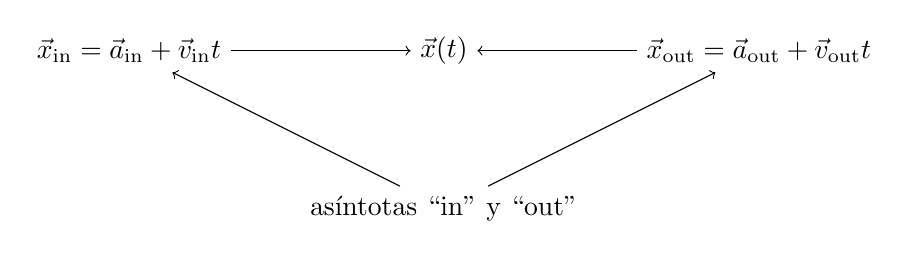
\begin{tikzpicture}[node distance=2cm, auto]
    % Nodes
    \node (xin) at (0, 0) {$\vec{x}_{\text{in}} = \vec{a}_{\text{in}} + \vec{v}_{\text{in}} t$};
    \node (xt) at (4, 0) {$\vec{x}(t)$};
    \node (asymp) at (4, -2) {asíntotas ``in'' y ``out''};
    \node (xout) at (8, 0) {$\vec{x}_{\text{out}} = \vec{a}_{\text{out}} + \vec{v}_{\text{out}} t$};
    
    % Arrows
    \draw[->] (xin) -- (xt) node[midway, above] {};
    \draw[<-] (xin) -- (asymp) node[midway, left] {};
    \draw[<-] (xt) -- (xout) node[midway, above] {};
    \draw[->] (asymp) -- (xout) node[midway, right] {};
\end{tikzpicture}

Si la partícula se aproxima al blanco siguiendo una asíntota 'in', la trayectoria de colisión queda completamente definida. No todas las trayectorias definen asíntotas 'in' y 'out', también existen trayectorias correspondientes a estados ligados.\\ \\
En Mecánica Cuántica, una trayectoria de colisión vendrá descrita por un 'ket' que evoluciona de acuerdo a la ecuación de Schrödinger,
\begin{equation}
    i\hbar\frac{d\ket{\Psi(t)}}{dt}=H\ket{\Psi(t)}\hspace{5mm}\text{con}\hspace{5mm}H=\frac{P^2}{2m}+V(\vec{x})=H^0+V(\vec{x})
\end{equation}
Tomamos $\ket{\Psi(t=0)}=\ket{\Psi}$ y $\ket{\Psi(t)}=U(t)\ket{\varphi}=e^{-\frac{i}{\hbar}Ht}\ket{\Psi}$, siendo $U(t)$ el operador de evolución temporal. Ahora supongamos que la colisión tiene lugar 'cerca' de $t=0$ y que en $t\to\pm\infty$ la partícula es libre, tal que
\[\ket{\Psi(t)}\underset{t\to\underset{(+)}{-}\infty}{\longrightarrow}\ket{\Psi_{\underset{(out)}{in}}(t)}\]
donde $\ket{\Psi_{\underset{(out)}{in}(t)}}$ evoluciona como una partícula libre, $H^0$, así
\begin{center}
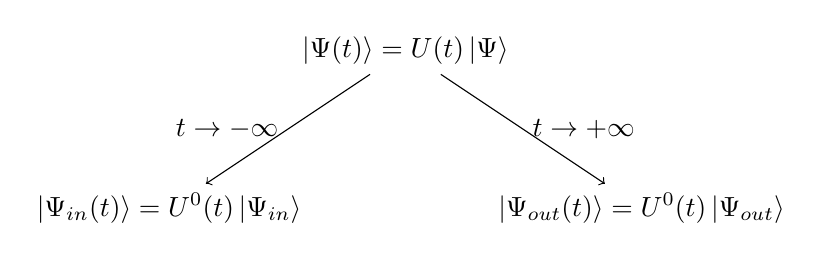
\begin{tikzpicture}[node distance=2cm, auto]
    % Nodes
    \node (xin) at (0, 0) {$\ket{\Psi(t)}=U(t)\ket{\Psi}$};
    \node (xt) at (-3, -2) {$\ket{\Psi_{in}(t)}=U^0(t)\ket{\Psi_{in}}$};
    \node (asymp) at (3, -2) {$\ket{\Psi_{out}(t)}=U^0(t)\ket{\Psi_{out}}$};
   % \node (xout) at (8, 0) {$\vec{x}_{\text{out}} = \vec{a}_{\text{out}} + \vec{v}_{\text{out}} t$};
    
    % Arrows
    \draw[->] (xin) -- (xt) node[midway, left] {$t\to-\infty$};
    \draw[->] (xin) -- (asymp) node[midway, right] {$t\to+\infty$};
    %\draw[<-] (xt) -- (xout) node[midway, above] {};
    %\draw[->] (asymp) -- (xout) node[midway, right] {};
\end{tikzpicture}
\end{center}
donde $\ket{\Psi_{in}}$ y $\ket{\Psi_{out}}$ son los estados asintóticos 'in' y 'out'.
\section{Colisión asintótica. Operador de colisión o matriz S}
Para tener una teoría de colisiones bien definida, $V(\vec{x})$ debe satisfacer las siguientes condiciones,
\begin{enumerate}[label=(\roman*)]
    \item Los estados asintóticos no se comportan como partículas libres, es decir,
    \[\frac{V(r)}{1/r^3}\underset{r\to\infty}{\longrightarrow}0\]
    \item Puede divergir en $r\to0$, pero más despacio que $1/r^{3/2}$ o puede producirse 'captura', es decir,
    \[\frac{V(r)}{1/r^{3/2}}\underset{r\to0}{\longrightarrow}0\]
    \item $V(r)$ debe ser continuo para todos los valores de $r$, excepto (posiblemente) en un número finito de discontinuidades.
\end{enumerate}

\textbf{Condición asintótica:} bajo estas tres condiciones, se puede demostrar que hay una correspondencia 1 a 1 entre estados asintóticos $\ket{\Psi_{in}}$ y $\ket{\Psi_{out}}$.
\begin{theorem}
    Si el potencial $V(r)$ satisface estas condiciones, para cada $\ket{\Psi_{in}}$ hay un único estado de colisiones $\ket{\Psi}$, tal que $\ket{\Psi(t)}-\ket{\Psi_{in}(t)}=U(t)\ket{\Psi}-U^0(t)\ket{\Psi_{in}}\underset{t\to-\infty}{\longrightarrow}0$, entonces
    \[\ket{\Psi}=\lim_{t\to-\infty}U^{\dagger}(t)U^0(t)\ket{\Psi_{in}}\equiv\Omega_+\ket{\Psi_{in}}\]
    donde $\Omega$ es el operador de Möller.\\
    Análogamente, hay un único $\ket{\Psi_{out}}$ tal que
    \[U(t)\ket{\Psi(t)}-U^0(t)\ket{\Psi_{out}}\underset{t\to+\infty}{\longrightarrow}0\Rightarrow\ket{\Psi}=\lim_{t\to+\infty}U^{\dagger}(t)U^0(t)\ket{\Psi_{out}}\equiv\Omega_-\ket{\Psi_{out}}\]
\end{theorem}
Los operadores de Möller $\Omega_{\pm}$ relacionan los estados asintóticos a $t=0$ con el estado de colisión a $t=0$, tal que
\begin{Figura}
    \centering
    \includegraphics[width=0.8\linewidth]{col4.png}
    \captionof{figure}{Esquema.}
    \label{fig7.4}
\end{Figura}
Por tanto,
\[\Omega_+=\lim_{t\to-\infty}U^{\dagger}(t)U^0(t);\hspace{6mm}\Omega_-=\lim_{t\to+\infty}U^{t}U^0(t)\]
Veamos si $\Omega_{\pm}$ es unitario, es decir, si $\Omega_{\pm}^{\dagger}\Omega_{\pm}=\mathbb{I}$:\\ \\
-Tomamos $\ket{\Psi_{\underset{(out)}{in}}(t)}$ que representa cualquier estado del espacio de Hilbert, y tomamos $\ket{\Psi}$ que representa un estado de colisiones a $t=0$, pero estos no son cualquier estado del espacio de Hilbert, sino que pertenece a $R_+$. Por tanto,
\[D(\Omega_+)=\mathscr{H}\]
\[R(\Omega_+)=R_+=R(\Omega_-)\]
\[\mathscr{H}=R_++B\]
Por tanto,
\[\Omega_+^{\dagger}\Omega_+\ket{\Psi_{in}}=\ket{\Psi_{in}}\]
luego, como $\Omega_+\ket{\Psi_{in}}\in R_+\land\notin\mathscr{H}$, se dice que $\Omega_+^{\dagger}$ es \textit{isosimétrico}, es decir, es unitario sobre $R_+$, pero no lo es sobre todo $\mathscr{H}$. Análogamente tenemos lo mismo para $\Omega_-^{\dagger}$ y $\Omega_-$.\\ \\
Usando que $\Omega_+\ket{\Psi_{in}}=\ket{\Psi}=\Omega_-\ket{\Psi_{out}}$, multiplicamos por $\Omega_-^{\dagger}$ por la izquierda,
\[\Omega_-^{\dagger}\Omega_-\ket{\Psi_{out}}=\ket{\Psi_{out}}=\Omega_-^{\dagger}\Omega_+\ket{\Psi_{in}}\]
Por tanto, tenemos la relación entre $\ket{\Psi_{in}}$ y $\ket{\Psi_{out}}$ tal que
\begin{equation}
    \ket{\Psi_{out}}=\Omega_-^{\dagger}\Omega_+\ket{\Psi_{in}}
\end{equation}
Luego, definimos el operador $S\equiv\Omega_-^{\dagger}\Omega_+$, tal que $\ket{\Psi_{out}}=S\ket{\Psi_{in}}$, denominado \textit{operador de colisión} (scattering) o \textit{matriz }$S$.\\ \\
Si antes de la colisión el estado 'es' $\ket{\Psi_{in}}$, tras la colisión pasa a 'ser' $\ket{\Psi_{out}}$ y $S$ es un operador unitario, así, $D(S)=R(S)=\mathscr{H}$. Luego, $S$ es todo lo que podemos calcular en una colisión, pues si enviamos $\ket{\Psi_{in}}$, tras la colisión tendremos el estado $\ket{\Psi_{out}}=S\ket{\Psi_{in}}$.\\ \\
Por otro lado, la probabilidad de que el estado $\ket{\Psi_{in}}$ se transforme, tras la colisión, en el estado $\ket{\Phi_{out}}$ es,
\begin{equation}
    \omega(\Psi_{in}\to\Phi_{out})=\abss{\braket{\Phi_{out}|\Psi_{in}}}=\abss{\Phi_{out}|S|\Psi_{in}}
\end{equation}
\section{Conservación de la energía}
Tenemos el Hamiltoniano $H=\frac{P^2}{2m}+V(r)$ que es independiente del tiempo $t$, por lo que el valor esperado de la energía para el estado $\ket{\Psi(t)}$ es constante, es decir, $\frac{d\ket{\Psi(t)}}{dt}=0$ y entonces, la energía de los estados asintóticos 'in' y 'out' debe ser la misma, tal que
\[\begin{array}{cl}
    E_{in} & =\braket{\Psi_{in}|H^0|\ket{\Psi_{in}}} \\
    || & \\
    E_{out} & =\braket{\Psi_{out}|H^0|\Psi_{out}}=\braket{\Psi_{in}|S^{\dagger}H^0S|\Psi_{in}}
\end{array}\]
Por tanto,
\[H^0=S^{\dagger}H^0S\Longrightarrow SH^0=H^0S\longrightarrow\brackets{S,H^0}=0\]
Además, podemos expresar $\ket{\Psi_{out}}$ en términos de $\ket{\Psi_{in}}$ en la representación de momentos, tal que
\begin{equation}
    \Psi_{out}(\vec{p}')=\braket{\vec{p}'|\Psi_{out}}=\braket{\vec{p}'|S'\Psi_{in}}=\int d^3p\braket{\vec{p}'|S|\vec{p}}\Psi_{in}(\vec{p})
\end{equation}
donde los $\braket{\vec{p}'|S|\vec{p}}$ son los elementos de la matriz $S$ en la representación de momentos. Luego, tenemos la función de onda 'out' en términos de la función de onda 'in' en la representación de momentos.\\ \\
Si el estado 'in' tiene momento bien definido, entonces
\begin{equation}
    \ket{\Psi_{in}}=\ket{\vec{p}}\Longrightarrow\Psi_{out}(\vec{p}')=\braket{\vec{p}'|S|\Psi_{in}}=\braket{\vec{p}'|S|\vec{p}}
\end{equation}
siendo $\braket{\vec{p}'|S|\vec{p}}$ la amplitud de probabilidad de obtener un estado 'out' con $\vec{p}'$, partiendo de un estado 'in' con $\vec{p}$.

\section{Matriz T on-shell y amplitud de colisión}
Como $S$ y $H^0$ conmutan, tenemos que
\[0=\braket{\vec{p}'|\brackets{H^0,S}|\vec{p}}=\braket{\vec{p}'|(H^0S-SH^0)|\vec{p}}=(E_{p'}-E_p)\braket{\vec{p}'|S|\vec{p}}\]
Si $E_{p'}\neq E_p$, entonces $\braket{\vec{p}'|S|\vec{p}}=0$, cosa que no tiene sentido porque no tendríamos colisión. Por lo que debemos usar la conservación de la energía, de forma que si $\vec{p}$ cambia a $\vec{p}'\neq\vec{p}$ con $|\vec{p}'|=|\vec{p}|$, tenemos que $E_{p'}=E_p$.\\ \\
Podemos parametrizar los elementos de $S=\mathbb{I}+R$ tal que
\[\braket{\vec{p}'|S|\vec{p}}=\delta^3(\vec{p}'-\vec{p})-2\pi i\delta(E_{p'}-E_p)t(\vec{p}',\vec{p})\]
donde $\delta(E_{p'}-E_p)$ representa la conservación de la energía y $t(\vec{p}',\vec{p})$ son los elementos de la matriz $T$ on-shell. Además, se define la amplitud de colisión como
\begin{equation}
    f(\vec{p}',\vec{p})=-(2\pi)^2\hbar^2mt(\vec{p}',\vec{p})
\end{equation}
donde $f(\vec{p}',\vec{p})$ y $t(\vec{p}',\vec{p})$ son funciones equivalentes usadas en la literatura par describir las colisiones. En términos de $f(\vec{p}',\vec{p})$, la parametrización de los elementos de $S$ queda,
\begin{equation}
    \braket{\vec{p}'|S|\vec{p}}=\delta^3(\vec{p}'-\vec{p})+\frac{i}{2\pi\hbar m}\delta(E_{p'}-E_p)f(\vec{p}',\vec{p})
\end{equation}
y el estado $\Psi_{out}(\vec{p}')$ queda,
\begin{equation}
    \Psi_{out}(\vec{p}')=\int d^3`\braket{\vec{p}'|S|\vec{p}}\Psi_{in}(\vec{p})=\Psi_{in}(\vec{p}')+\frac{i}{2\pi\hbar m}\int d^3p\delta(E_{p'}-E_p)f(\vec{p}',\vec{p})\Psi_{in}(\vec{p})
\end{equation}

\section{Sección eficaz}
\subsection{Sección eficaz clásica}
Consideramos una colisión donde enviamos un proyectil con $\vec{p}_0$ contra un sólido rígido, tal que
\begin{Figura}
    \centering
    \includegraphics[width=0.8\textwidth]{col5.png}
    \captionof{figure}{Colisión clásica.}
    \label{fig7.5}
\end{Figura}
Suponemos que enviamos muchos proyectiles con una distribución aleatoria de parámetro de impacto $\vec{\rho}$ y momento $\vec{p}_0$, teniendo un \textit{haz de partículas}. Enviamos $n_{inc}$ proyectiles por unidad de área, perpendiculares a $\vec{p}_0$. Se define la sección eficaz total $\sigma$ en esta colisión como,
\begin{equation}
    N_{SC}=n_{inc}\cdot\sigma
\end{equation}
donde $\sigma$ tiene unidades de área y $N_{SC}$ representa el número de partículas que colisionan. Esto podemos verlo mejor representando la proyección del sólido rígido, tal que
\begin{Figura}
    \centering
    \includegraphics[width=0.8\textwidth]{col6.png}
\end{Figura}
Por tanto, las partículas que chocarán con el sólido rígido serán las partículas que pasen por la proyección del sólido rígido $A$. Luego, en mecánica clásica $\sigma=A$.\\ \\
Se suele usar de unidades el milibar, $1$ mb$=10^{-27}$ cm$^2$, pues es más o menos el tamaño de un protón.\\ \\
La sección eficaz $\sigma$ da un primer observable en la colisión, que nos dice cuántas partículas chocan.\\ \\
Un observable más general es cuántas partículas chocan y salen en una dirección particular. Para ello, debemos saber cómo se especifica una dirección:
\begin{multicols}{2}
    \begin{Figura}
        \centering
        \includegraphics[width=0.6\textwidth]{col7.png}
    \end{Figura}
    -Una dirección viene especificada por $\theta$.\\ \\
    -Un intervalo de colisiones viene especificado por un ángulo $\Delta \theta$ que verifica $\Delta l=\Delta\theta\cdot r$. Por tanto,
\begin{equation}
    \Delta\theta=\frac{\Delta l}{r}
\end{equation}
que se mide en radianes. Para todas las direcciones tendremos que $\Delta\theta=\frac{2\pi r}{r}=2\pi $ rad. Si pasamos a infinitésimos tenemos $dl=d\theta\cdot r$.
\end{multicols}

Pasando a 3 dimensiones,
\begin{multicols}{2}
    \begin{Figura}
        \centering
        \includegraphics[width=0.8\textwidth]{col8.png}
    \end{Figura}
    -Para especificar las direcciones necesitamos 2 parámetros, $(\theta,\varphi)=\Omega$.\\ \\
    -El intervalo de direcciones viene dado por el ángulo sólido $\Delta\Omega$, el 'cono'.\\ \\
    -Se cumple que
    \[\Delta S=\Delta\Omega \cdot r^2\Rightarrow\Delta\Omega=\frac{\Delta S}{r^2}\]
    Para todas las direcciones tenemos $\Delta\Omega=\frac{4\i r^2}{r^2}=4\pi $ sr (unidad de ángulos en 3-dim).
\end{multicols}
Podemos medir cuántas partículas $\Delta N_{SC}$ salen en la dirección $\Delta\Omega$, o la densidad de partículas en esa dirección, tal que
\[\brackets{\frac{\text{partículas}}{\text{sr}}}\lim_{\Delta\Omega\to0}\frac{\Delta N_{SC}}{\Delta\Omega}=\frac{dN_{SC}}{d\omega}=n_{inc}\frac{d\sigma}{d\Omega}\]
donde $\frac{d\sigma}{d\Omega}$ es la sección eficaz diferencial. \\ \\
Podemos ver cuántas partículas salen en $\Delta\Omega=\Delta\varphi\Delta(\cos\theta)$, tal que
\[\left.N_{SC}\right|_{\Delta\Omega}=\int_{\Delta\Omega}d\Omega n_{inc}\frac{d\sigma}{d\Omega}=n_{inc}\int_{\Delta(\cos\theta)}d(\cos\theta)\int_{\Delta\varphi}d\varphi\frac{d\sigma}{d\Omega}(\theta,\varphi)\]
en todas las direcciones tendremos que $N_{SC}=n_{inc}\sigma$, por tanto,
\begin{equation}
    \sigma=\int_{-1}^1d(\cos\theta)\int_0^{2\pi}d\varphi\frac{d\sigma}{d\Omega}
\end{equation}

\subsection{Sección eficaz en mecánica cuántica}
En mecánica cuántica tenemos un estado asintótico 'in' contra el blanco $\Psi_{in}(\vec{p})=\braket{\vec{p}|\Psi_{in}}$; tras la colisión, tenemos el estado $\ket{\Psi_{out}}$, con función de onda $\Psi_{out}(\vec{p}')=\braket{\vec{p}'|\Psi_{out}}$. Por tanto, nos preguntamos cuál es la probabilidad de encontrar el estado 'out' en el cono de direcciones $d\Omega_{p'}$,
que será,
\begin{equation}
    \omega(\Psi_{in}\to d\Omega_{p'})=d^3p'\abss{\Psi_{out}(p')}=d\Omega_{p'}\int_0^{\infty}p^{'2}dp'\abss{\Psi_{out}(p')}
\end{equation}
donde hemos usado que $d^3p'=\int\limits_0^{\infty}p^{'2}dp'd\Omega_{p'}$, pues representa cualquier momento $p'$ dentro del cono $d\Omega_{p'}$.\\ \\
Supongamos que enviamos un haz de partículas; cada una de ellas descrita por una función de onda en la representación de momentos muy 'cercana' a $\vec{p}_0$, con parámetro de impacto $\vec{\rho}$ aleatorio y una densidad de $n_{inc}$ partículas por unidad de área perpendicular a $\vec{p}_0$. También asumimos que la interacción entre las partículas del haz es despreciable. Entonces, definimos la sección eficaz diferencial como
\begin{equation}
    \frac{dN_{SC}}{d\Omega_{p'}}=n_{inc}\frac{d\sigma}{d\Omega_{p'}};\hspace{6mm}\left.N_{SC}\right|_{\Delta\Omega}=\int d\Omega n_{inc}\frac{d\sigma}{d\Omega}\Rightarrow\frac{d\sigma}{d\Omega}=\abss{f(\vec{p}',\vec{p}_0}=(2\pi)^4\hbar^2m^2\abss{t(\vec{p}',\vec{p}_0)}
\end{equation}
Así, si somos capaces de calcular $S$ o $f(\vec{p}',\vec{p}_0)$ para un potencial $V(\vec{r})$ dado, podemos deducir la sección eficaz diferencial.
\section{Teorema óptico}
Es una consecuencia de la unitariedad de la matriz $S$, tal que
\[S^{\dagger}S=\mathbb{I}\Rightarrow(\mathbb{I}+R)^{\dagger}(\mathbb{I}+R)=\mathbb{I}\Rightarrow R_+R^{\dagger}=-R^{\dagger}R\]
Por tanto,
\[\begin{array}{ccccc}
\braket{\vec{p}'|R|\vec{p}}&+&\braket{\vec{p}'|R^{\dagger}|\vec{p}}&=&-\braket{\vec{p'}|R^{\dagger}R|\vec{p}}  \\
    || & & || & &  \\
    \frac{i}{2\pi\hbar m}\delta(E_p-E_{p'})f(\vec{p}',\vec{p}) & & \braket{\vec{p}|R|\vec{\rho}}^* & &
\end{array}\]
Luego, introduciendo la identidad como $\int d^3p''\ket{\vec{p}''}\bra{\vec{p}''}$ en la derecha de la igualdad, tenemos
\[\frac{i}{2\pi\hbar m}\delta(E_{p'}-E_p)\brackets{f(\vec{p}',\vec{p})-f(\vec{p},\vec{p}')^*}=\left(\frac{i}{2\pi\hbar m}\right)^2\int d^3p''\delta(E_{p''}-E_{p'})\delta(E_{p''}-E_p)f(\vec{p}'',\vec{p}')^*f(\vec{p}'',\vec{p})\overset{*}{=}\]
Teniendo así un $0=0$ para todos los valores, salvo para $E_{p'}=E_p$. Luego, la integral en $\vec{p}''$ impone que $p''=p$. Así, queda 
\[\overset{*}{=}\frac{i}{2\pi\hbar m}\int p^{''2}dp''d\omega_{p''}\delta(E_{p''}-E_p)f(\vec{p}'',\vec{p}')^*f(\vec{p}'',\vec{p})\]
Así tenemos que,
\[f(\vec{p}',\vec{p})-f(\vec{p}.\vec{p}')^*=\frac{i}{2\pi\hbar m}p^2\frac{m}{p}\int d\Omega_{p'}f(\vec{p}'',\vec{p}')^*f(\vec{p}'',\vec{p})\]
Tomamos $\vec{p}=\vec{p}'$,
\[\underbrace{f(\vec{p},\vec{p})-f(\vec{p},\vec{p})^*}_{2iImf(\vec{p},\vec{p})}=\frac{i}{2\pi\hbar}p\underbrace{\int d\Omega_{p''}\overbrace{\abss{f(\vec{p}'',\vec{p}}}^{\frac{d\sigma}{dp}}}_{\sigma_{total}}\]
Por tanto,
\begin{equation}
    Imf(\vec{p},\vec{p})=\frac{p}{4\pi\hbar}\sigma(\vec{p})
\end{equation}
siendo éste el \textbf{Teorema Óptico}. Por tanto, la parte imaginaria de la amplitud de colisión 'forward' (hacia delante) es proporcional a la sección eficaz total.\\ \\
Vemos que la amplitud de colisión no es real; tiene una parte imaginaria positiva en la dirección forward. Así, dada una sección eficaz diferencial fija, el Teorema Óptico permite deducir la parte real e imaginaria de $f$ en $\vec{p}=\vec{p}'$.

\section{El operador de Green y el operador T}
Partiendo del potencial $V(\vec{r})$, obtenemos $f(\vec{p}',\vec{p})$ y así, obtenemos $t(\vec{p}',\vec{p})=\lim_{\epsilon\to0}\braket{\vec{p}'|T(E_++iz)|\vec{p}}$.\\ \\
Por un lado, los operadores de Green de los Hamiltonianos $H^0=\frac{P^2}{2m}$ y $H=H^0+V$ serán
\[G^0(z)=(z-H^0)^{-1}=\frac{1}{z-H^0}\]
\[G(z)=(z-H)^{-1}=\frac{1}{z-H}\]
con $z\in\mathbb{C}$. Por tanto, $(z-H^0)G^0(z)=\mathbb{I}$ con $\braket{\vec{x}|H^0|\Psi}=-\frac{\hbar^2\nabla^2}{2m}\braket{\vec{x}|\Psi}$. Por tanto,
\[\left(\frac{\hbar^2\nabla^2}{2m}+z\right)\braket{\vec{x}|G^0(z)|\vec{x}'}=\delta^3(\vec{x}-\vec{x}')\]
donde $\braket{\vec{x}|G^0(z)|\vec{x}'}$ es la función de Green del operador $\frac{\hbar^2\nabla^2}{2m}+z$.\\ \\
Análogamente,
\begin{equation}
    \left(\frac{\hbar^2\nabla^2}{2m}+V(\vec{x})+z\right)\braket{\vec{x}|G(z)|\vec{x}'}=\delta^3(\vec{x}-\vec{x}')
\end{equation}
\begin{remark}
    \begin{itemize}
        \item $G(z)$ no está definido para $z=E_n$, pues como $H\ket{n}=E_n\ket{n}$, entonces $\frac{1}{E_n-H}\ket{n}$ diverge.
        \item En la base de autovectores de $H$,
        \[G(z)=\frac{1}{z-H}\sum_n\ket{n}\bra{n}=\sum_n\frac{\ket{n}\bra{n}}{x-E_n}=\int dE\frac{\ket{n}\bra{n}}{z-E}\]
        donde pasamos a la integral solo si la base es continua.
        \item Podemos relacionar $G(z)$ y $G^0(z)$ usando,
        \[A^{-1}=B^{-1}+B^{-1}(B-A)A^{-1}\]
        tomamos $A=z-H=z-H^0-V$ y $B=z-H^0$, luego $B-A=V$, por tanto,
        \[A^{-1}=\frac{1}{z-H}=G(z)=B^{-1}+B^{-1}(B-A)A^{-1}=\frac{1}{a-H^0}+\frac{1}{z-H^0}VG(z)=G^0(z)+G^0(z)VG(z)\]
        luego,
        \begin{equation}
            G(z)=G^0(z)+G^0(z)VG(z)
        \end{equation}
        siendo la ecuación de Lippmann-Scwiger (L-S) para $G(z)$. Por tanto,
        \[G^0(z)\ket{\vec{p}}=(z-H^0)^{-1}\ket{\vec{p}}=\frac{1}{z-E_p}\ket{\vec{p}}\]
        con $E_p=\frac{P^2}{2m}$.
    \end{itemize}
\end{remark}
Por otro lado, se define el operador $T(z)$ como
\begin{equation}
    T(z)=V+VG(z)V
\end{equation}
siendo una función analítica en el plano complejo, excepto en los autovalores de la energía $(z\neq E_n)$. Usando la ecuación L-S, tenemos
\begin{equation}
    G^0T=\underbrace{(G^0+G^0VG^0)}_{L-S}V=GV
\end{equation}
Por tanto,
\begin{equation}
    T(z)=V+VG^0(z)T(z)
\end{equation}
siendo la ecuación de L-S para $T(z)$.
\\ \\
Además, podemos relacionar los operadores $G(z)$ y $T(z)$ con $\Omega_{\pm}$ y $S$ de la siguiente forma,
\begin{equation}
    t(\vec{p}',\vec{p})=-\frac{1}{(2m)^2\hbar m}f(\vec{p}',\vec{p})=\lim_{\epsilon\to0^+}\braket{\vec{p}'|T(E_p+i\epsilon)|\vec{p}}
\end{equation}
\subsection{Serie de Born}
Nuestro objetivo ahora es resolver el braket $\braket{\vec{p}'|T(E_p+i\epsilon)|\vec{p}}$ a partir de $T=V+VG^0T$. La serie de Born resuelve la ecuación de L-S de forma perturbativa, a partir del Hamiltoniano $H=H^0+\lambda V$, donde $\lambda$ es una 'constante de acoplo' que factorizamos en el potencial, donde si $\lambda=0$ tenemos partículas libres y si $\lambda<<<1$, tenemos interacciones débiles.\\ \\
Se asume que $T(z)$ puede expandirse en serie de potencias de $\lambda$, tal que
\[T(z)=\sum_{n=0}^{\infty}\lambda^nT^{(n)}(z)=T^{(0)}(z)+\lambda T^{(1)}(z)+\lambda^2T^{(2)}(z)+\dots\]
Sustituyendo esta serie en la ecuación de L-S para $T(z)$ tenemos,
\[T^{(0)}(z)+\lambda T^{(1)}(z)+\lambda^2T^{(2)}(z)+\dots=\lambda V+\lambda V G^0(T^{(0)}(z)+\lambda T^{(1)}(z)+\lambda^2T^{(2)}(z)+\dots)\]
Luego,
\[\left.\begin{array}{rcl}
    T^{(0)} & = & 0 \\
    T^{(1)} & = & V+VG^0T^{(0)}=V\\
    T^{(2)} & = & VG^0V\\
    \vdots & & \\
    T^{(n)} & = & (VG^0)^{n-1}V
\end{array}\right\rbrace\Rightarrow T(z)=V+VG^0(z)V+\dots\]
siendo la serie de Born, que es una serie de potencias de $\frac{V}{E_p+i\epsilon-H^0}$.\\ \\
La aproximación de Born es hacer $T\approx V$; siendo buena aproximación si cumple:
\begin{enumerate}[label=(\roman*)]
    \item que el acoplo $\lambda$ sea pequeño (régimen de acoplamiento débil).
    \item o que la energía cinética sea grande $(E_p>>V)$ (régimen de altas energías).
\end{enumerate}
En esta aproximación tenemos que
\begin{equation}
    \begin{array}{rl}
        f(\vec{p}',\vec{p}) & =f^{(1)}(\vec{p}',\vec{p}=-(2\pi)^2\hbar m\braket{\vec{p}'|V|\vec{p}}=-(2\pi)^2\hbar m\int d^3\vec{x}\braket{\vec{p}'|V|\vec{x}}\braket{\vec{x}|\vec{p}}  \\
         & =-\frac{(2\pi)^2\hbar m}{(2\pi\hbar)^3}\int d^3xV(x)e^{-\frac{i}{\hbar}\vec{q}\cdot\vec{x}}=f(\vec{q})
    \end{array}
\end{equation}
donde $\vec{q}=\vec{p}'-\vec{p}$ es el momento transferido. Además, si el ángulo entre $\vec{p}'$ y $\vec{p}$ es $\theta$, entonces tenemos que $q=2`\sin(\theta/2)$.\\ \\
Suponiendo un potencial central $V(\vec{x})=V(r)$ tenemos,
\begin{equation}
    f(\vec{p}',\vec{p})\approx f(\vec{q})=f(p,\theta)=-\frac{m}{2\pi\hbar^2}\int_0^{\infty}dr\cdot r^2V(r)\int_0^{2\pi}d\varphi\int_{-1}^1d(\cos\tilde{\theta})e^{-\frac{i}{\hbar}qr\cos\tilde{\theta}}=
\end{equation}
\[=-\frac{m}{2\pi\hbar^2}\int_0^{\infty}dr\cdot r^2\frac{2\hbar}{qr}\sin\left(\frac{qr}{\hbar}\right)V(r)2\pi=-\frac{2m}{q\hbar}\int_0^{\infty}dr\cdot r\sin\left(\frac{qr}{\hbar}\right)V(r)\]
\begin{itemize}
    \item Si $\vec{p}'=\vec{p}$ tenemos la amplitud de colisión forward,
    \begin{equation}
        f^{(1)}(\vec{p},\vec{p})\overset{\curlybraces{\sin\theta\approx\theta}}{\approx}-\frac{2m}{\hbar^2}\int dr\cdot r^2V(r)
    \end{equation}
    siendo independiente de $p$.
    \item Si $p$ es grande, estamos en el límite de altas energías, y entonces $f^{(1)}(\vec{p}',\vec{p})$ va acero como $1/p$ en todas las direcciones de $\theta$, excepto cuando $\theta$ es forward $(\theta=0)$.
    \item La aproximación de Born 'viola' el Teorema Óptico, pues
    \[Imf(\vec{p},\vec{p})=\frac{p}{4\pi\hbar}\int d\omega\abss{f}=\frac{p}{4\pi\hbar}\sigma\Rightarrow f^{(1)}(\vec{p},\vec{p})\in\mathbb{R}\]
    pero esto se explica porque en la aproximación de Born solo usamos orden 1, y esto lo único que nos dice es que, a primer orden, la parte imaginaria es cero y la real no. Pero si considerásemos todos los órdenes, sí se satisfacería el Teorema Óptico.
\end{itemize}

\section{Ondas planas y ondas esféricas}
Una onda plana de momento $\vec{p}$ es una autofunción de momento bien definido y de energía cinética $H^0=\frac{P^2}{2m}$, también bien definida, con
\[\vec{p}(\vec{x})=\braket{\vec{x}|\vec{p}}=\frac{1}{(2\pi\hbar)^{3/2}}e^{\frac{i}{\hbar}\vec{p}\cdot\vec{x}}\]
propia de $\vec{p}$ y $H^0$.\\ \\
Sin embargo, $H^0$ también conmuta con $L^2$ y $L_z$, entonces podemos también definir una base de autoestados de $H^0,L_z,L^2$ (no de $P_i$, pues no conmuta con $L_z$ ni $L^2$, y no estaría bien definido). Sus componentes serán los vectores del tipo $\ket{\begin{matrix}
    E & l & m 
\end{matrix}}$, que representan \textit{ondas esféricas}.\\ \\
Las ondas esféricas son una base ortonormal de $\mathscr{H}$, especialmente, se usan para estudiar sistemas con simetría esférica, es decir, $V=V(r)$.\\ \\
Es sencillo deducir (imponiendo condición de ortogonalidad) los coeficientes del cambio de base, tal que
\[\ket{\begin{matrix}
    E & l & m 
\end{matrix}}=\int d^3p\ket{\vec{p}}\frac{1}{\sqrt{mp}}\delta\left(\frac{P^2}{2m}-E\right)Y_l^m(\vec{u}_p)\]
siendo una integral sobre todas las ondas planas, con $\vec{p}=p\vec{u}_p$. O también,
\[\ket{\vec{p}}=\sum_{l=0}^{\infty}\sum_{m=-l}^{+l}\left.\ket{\begin{matrix}
    E & l & m 
\end{matrix}}\right|_{E=\frac{P^2}{2m}}\frac{1}{\sqrt{mp}}Y_l^m(\vec{u}_p)^*\]
Además, como $\ket{\vec{p}}$ se relaciona con $\ket{\vec{x}}$, podemos relacionar $\ket{\begin{matrix}
    E & l & m 
\end{matrix}}$ con $\ket{\vec{x}}$, tal que
\[\varphi_{Elm}(\vec{x})=\braket{\vec{x}|\begin{matrix}
    E & l & m 
\end{matrix}}=\frac{(i)^l}{\hbar}\sqrt{\frac{2mp}{\pi\hbar}}J_l\left(\frac{pr}{\hbar}\right)Y_l^m(\vec{u}_x)\]
donde $J_l(x)$ es una función esférica de Bessel de orden $l$, que cumplen que
\[\lim_{x\to\infty}J_l(x)=\frac{1}{x};\hspace{6mm}\lim_{x\to0}J_l(x)=\frac{x^l}{(2l+1)!!}\]
donde $n!!=n(n-2)(n-4)\cdot\cdot\cdot2$ se denomina segundo factorial.\\ \\
También podemos expresar una onda plana como combinación de ondas esféricas, tal que
\[\frac{1}{(2\pi\hbar)^{3/2}}e^{\frac{i}{\hbar}\vec{p}\cdot\vec{x}}=\braket{\vec{x}|\vec{p}}=\overset{\curlybraces{\begin{matrix}
    \vec{x}=r\vec{u}_x\\
    \vec{p}=p\vec{u}_p
\end{matrix}}}{=}\frac{1}{(2m\hbar)^{3/2}}\sum_l(2l+1)(i)^lJ_l\left(\frac{pr}{\hbar}\right)\mathscr{P}_l(\vec{u}_p\cdot\vec{u}_x)\]
donde $\mathscr{P}_l(x)$ son los polinomios de Legendre de orden $l$. Vemos que para $|\vec{x}|\to\infty$ tenemos,
\[\braket{\vec{x}|\vec{p}}\to\frac{1}{(2\pi\hbar)^{3/2}}\sum_{l=0}^{\infty}\mathscr{P}_l(\vec{u}_p\cdot\vec{u}_x)\brackets{(-1)^l\frac{e^{-\frac{i}{\hbar}pr}}{\frac{i}{\hbar}pr}+\frac{e^{\frac{i}{\hbar}pr}}{\frac{i}{\hbar}pr}}\]
donde el sumatorio representa una superposición de ondas parciales de momento angular $l$, el $(-1)^l$ representa una fase real, $\frac{e^{-\frac{i}{\hbar}pr}}{\frac{i}{\hbar}pr}$ representa la onda 'in' y $\frac{e^{\frac{i}{\hbar}pr}}{\frac{i}{\hbar}pr}$ representa la onda 'out'.\\ \\
Clásicamente no hay diferencia entre una onda plana y una onda esférica.
\subsection{Estados asintóticos que no evolucionan con el tiempo}
Cuando tenemos estados asintóticos que no evolucionan con el tiempo, podemos definir
\[\ket{\vec{p}_+}=\Omega_+\ket{\vec{p}}\doteq\Psi_p^+(\vec{x})\]
Vemos que cuando $r\to\infty$, tenemos que
\[\ket{\vec{p}_+}=\frac{1}{(2\pi\hbar)^{3/2}}\sum_{l=0}^{\infty}\left(l+\frac{1}{2}\right)\mathscr{P}_l(\vec{u}_p\cdot\vec{u}_x)\brackets{(-1)^l\frac{e^{-\frac{i}{\hbar}pr}}{\frac{i}{\hbar}}+\frac{e^{2i\delta_l}e^{\frac{i}{\hbar}pr}}{\frac{i}{\hbar}pr}}\]
donde $\delta_l$ es el desfaje de la onda.
\section{Matriz S para ondas parciales}
Aplicamos $S\ket{\Psi_{in}}=\ket{\Psi_{out}}$ sobre una onda esférica y el objetivo es ver el efecto de la colisión. Usando la conservación de la colisión con un potencial que:
\begin{enumerate}[label=(\roman*)]
    \item no depende del tiempo, entonces $\brackets{S,H^0}=0$, luego $S\ket{E}$ también tiene energía $E$, con $S\ket{E}=a\ket{E}$.
    \item es un potencial central, entonces $\brackets{S,L_i}=0=\brackets{S,L^2}$, con $S\ket{\begin{matrix}
        l & m
    \end{matrix}}=b\ket{\begin{matrix}
        l & m
    \end{matrix}}$, donde $b$ no depende de $m$, pues $\brackets{S,L_{\pm}}=0$.
\end{enumerate}
Además, $S$ es unitario, pues no cambia el módulo del vector, tal que
\begin{equation}
    S\ket{\begin{matrix}
        E & l & m
    \end{matrix}}=e^{2i\delta_l}\ket{\begin{matrix}
        E & l & m
    \end{matrix}}
\end{equation}
donde $\delta_l$ es un desfaje producido por el potencial $V(r)$ en la onda parcial $l$ de energía $E=\frac{P^2}{2m}$. Veamos cómo se relaciona $\delta_l$ con la amplitud de colisión $f(\vec{p}',\vec{p})$:
\begin{equation}
    \braket{\vec{p}'|(S-\mathbb{I})\vec{p}}=\frac{i}{2\pi\hbar m}\delta(E_{p'}-E_p)f(\vec{p}',\vec{p})
\end{equation}
Cambiamos de base multiplicando la identidad $\mathbb{I}=\sum\limits_{l,m}\int dE\ket{\begin{matrix}
    E & l & m
\end{matrix}}\bra{\begin{matrix}
    E & l & m
\end{matrix}}$, donde 
\[\brackets{\begin{matrix}
    E & l & m
\end{matrix}|\vec{p}}=\frac{1}{\sqrt{mp}}\delta\left(\frac{P^2}{2m}-E\right)Y_l^m(\vec{u}_p)^*\]
\[(S-\mathbb{I})\ket{\begin{matrix}
    E & l & m
\end{matrix}}=\left[e^{2i\delta_l}-1\right]\ket{\begin{matrix}
    E & l & m
\end{matrix}}\]
Por tanto,
\[\frac{i}{2\pi\hbar m}\delta(E_{p'}-E_p)f(\vec{p}',\vec{p})=\frac{1}{mp}\delta(E_{p'}-E_p)\sum_{l,m}Y_l^m(\vec{u}_{p'})\left(e^{2i\delta_l}-1\right)Y_l^m(\vec{u}_p)^*\]
Así,
\begin{equation}
    f(\vec{p}',\vec{p})=\frac{2\pi\hbar}{ip}\sum_{l,m}Y_l^m(\vec{u}_{p'})\left(e^{2i\delta_l}-1\right)Y_l^m(\vec{u}_p)^*
\end{equation}
Sabemos que $\vec{u}_p$ y $\vec{u}_{p'}$ forman un ángulo $\theta$ y que $\sum\limits_{m}Y_l^^m(\vec{u}_{p'})Y_l^m(\vec{u}_p)=\frac{2l+1}{4\pi}\mathscr{P}_l(\cos\theta)$. Por tanto,
\begin{equation}
    f(\vec{p}',\vec{p})=f(E,\theta)=\frac{\hbar}{2ip}\sum_{l=0}^{\infty}(2l+1)\left(e^{2i\delta_l}-1\right)\mathscr{P}_l(\cos\theta)
\end{equation}
Es útil definir la amplitud de colisión en la onda parcial $l$ como
\[f_l(E)=\frac{e^{2i\delta_l}-1}{2i}\frac{\hbar}{p}=\frac{e^{i\delta_l}\sin(\delta_l)\hbar}{\sqrt{2Em}}\]
Por tanto,
\begin{equation}
    f(E,\theta)=\sum_{l=0}^{\infty}(2l+1)f_l(E)\mathscr{P}_l(\cos\theta)
\end{equation}
Usando la ortogonalidad de los polinomios de Legendre tenemos que
\[f_l(E)=\frac{1}{2}\int_{-1}^1d(\cos\theta)f(E,\theta)\mathscr{P}_l(\cos\theta)\]
En la aproximación de Born, los desfajes deben ser pequeños, tal que
\[f_l(E)=\frac{e^{i\delta_l}\sin(\delta_l)\hbar}{p}\approx\frac{(1+i\delta_l)\delta_l\hbar}{p}\approx\frac{\delta_l\hbar}{p}\]
Podemos expresar la sección eficaz total $\sigma$ como la suma de las contribuciones de las ondas parciales, tal que
\begin{equation}
    \sigma(p)=\int d\Omega\abss{f(p,\theta)}=\sum_l\sigma_l(p)
\end{equation}
con $\sigma_l(p)=4\pi(2l+1)\abss{f_l(p)}=4\pi\hbar^2(2l+1)\frac{\sin^2\delta_l}{p^2}$.\\ \\
Como $|\sin\delta_l|\leq1$, entonces $\sigma_l(p)\leq4\pi\hbar^2\frac{2l+1}{p^2}$; siendo la condición de unitariedad para la contribución de la onda parcial $l$.
\subsection{Condición para usar la aproximación de Born}
Esta aproximación se podrá usar si se verifica que,
\[\left|\frac{m}{2\pi\hbar^2}\int d^3x'\frac{e^{\frac{i}{\hbar}pr'}e^{\frac{i}{\hbar}\vec{p}\cdot\vec{x}}}{r'}V(\vec{x})\right|<1\]
Esto se puede simplificar en algunos casos.\\ \\
-Suponiendo que $V(r)$ es despreciable para $r>a$, y que toma un valor máximo, $V_{max}$, entonces
\begin{enumerate}[label=(\roman*)]
    \item \textbf{Límite de bajas energías:} tenemos que $\frac{p}{\hbar}a<1$, entonces la fase no oscila, por lo que
    \[\left|\frac{m}{2\pi\hbar^2}\int d^3x'\frac{e^{\frac{i}{\hbar}pr'}e^{\frac{i}{\hbar}\vec{p}\cdot\vec{x}}}{r'}V(\vec{x})\right|<\frac{m}{2\pi\hbar^2}4\pi\int_0^adr'r^{'2}\frac{V_{max}}{r'}=\frac{2m}{\hbar^2}\frac{a^2}{2}V_{max}<1\]
    luego $V_{max}<\frac{\hbar^2}{a^2m}$ es un potencial débil.
    \item \textbf{Alta energía:} tenemos que $\frac{p}{\hbar}a>>1$, entonces
    \[\frac{m}{2\pi\hbar^2}\int_0^ar^{'2}dr'\int_0^{2\pi}d\varphi\int_{-1}^{1}\frac{e^{\frac{i}{\hbar}pr'(1+\cos\theta)}}{r'}V(\vec{x})\]
    Vemos que la fase oscila rápidamente; al hacer la integral comprobamos en todas partes menos en $\vec{p}\cdot\vec{x}=-pr$, luego tenemos que
    \[\left|\frac{m}{2\pi\hbar^2}\int d^3x'\frac{e^{\frac{i}{\hbar}pr'}e^{\frac{i}{\hbar}\vec{p}\cdot\vec{x}}}{r'}V(\vec{x})\right|<\frac{m}{\hbar^2}\int_0^adr'r'V_{max}\int_{-1-\hbar/pa}^{-1+\hbar/pa}d(\cos\theta)=\frac{m}{\hbar^2}\frac{a^2V_{max}2\hbar}{2pa}<1\]
\end{enumerate}
\section{Entregable}
\begin{enumerate}
\item \textbf{La amplitud de dispersión de una partícula con momento $p=200$ MeV/c es}
\[f(p,\theta,\varphi)=\frac{\hbar}{2p}\brackets{\left(1+3\frac{\sqrt{3}}{2}\cos\theta\right)+i\left(1+\frac{9}{2}\cos\theta\right)}\]
\begin{enumerate}
    \item \textbf{Calcula la sección eficaz total en mb (milibarns).}\\
    \textbf{[$\hbar c\approx200$ MeV fm, $1$ fm $=10^{-13}$ cm, $1$ mb$=10^{-27}$ cm$^2$]}
    \item \textbf{¿Se cumple el teorema óptico?}
    \item \textbf{Halla todos los desfajes}
\end{enumerate}
\end{enumerate}

\subsubsection*{Apartado (a)}
Sabemos que la sección eficaz total viene de integrar la sección eficaz diferencial, que es
\[\frac{d\sigma}{d\Omega}=\abss{f(p,\theta,\varphi)}=\abss{f(p,\theta,\varphi)=\frac{\hbar}{2p}\brackets{\left(1+3\frac{\sqrt{3}}{2}\cos\theta\right)+i\left(1+\frac{9}{2}\cos\theta\right)}}=\]
\[=\frac{\hbar^2}{4p^2}\brackets{\left(1+3\frac{\sqrt{3}}{2}\cos\theta\right)^2+\left(1+\frac{9}{2}\cos\theta\right)^2}=\frac{\hbar^2}{4p^2}\brackets{1+\frac{27}{4}\cos^2\theta+3\sqrt{3}\cos\theta+1+\frac{81}{4}\cos^2\theta+9\cos\theta}\]
\[=\frac{\hbar^2}{4p^2}\brackets{2+(9+3\sqrt{3})\cos\theta+27\cos^2\theta}\]

Por tanto, la sección eficaz total viene dada por,
\[\sigma=\int \frac{d\sigma}{d\Omega}d\Omega=\int_{-1}^{1}d(\cos\theta)\int_0^{2\pi}d\varphi\abss{f(p,\theta,\varphi)}=\frac{\cancel{2}\pi\hbar^2}{\cancel{4}p^2}\int_{-1}^{1}\brackets{2+(9+3\sqrt{3})\cos\theta+27\cos^2\theta}d(\cos\theta)=\]
\[=\frac{\hbar^2\pi}{2p^2}\brackets{2\int_{-1}^{1}d(\cos\theta)+(9+3\sqrt{3})\int_{-1}^{1}\cos\theta d(\cos\theta)+27\int_{-1}^1\cos^2\theta d(\cos\theta)}=\]
Vamos a hacer el cambio de variable $x=\cos\theta$.
\[=\frac{\hbar^2\pi}{2p^2}\brackets{2\int_{-1}^{1}dx+(9+3\sqrt{3})\int_{-1}^{1}x\cdot dx+27\int_{-1}^1x^2 dx}=\]
\[=\frac{\hbar^2\pi}{2p^2}\brackets{2\left. x\right|_{-1}^{1}+\frac{9+3\sqrt{3}}{2}\left. x^2\right|_{-1}^{1}+\frac{27}{3}\left.x^3\right|_{-1}^{1}}=\]
\[=\frac{\hbar^2\pi}{2p^2}\brackets{4+18}=\frac{22\hbar^2\pi}{2p^2}=\frac{11\pi(\hbar c)^2}{(pc)^2}\overset{\curlybraces{\begin{matrix}
    \hbar c\approx 200\text{ MeV fm}\\
    p=200 \text{ MeV/c }\\
    \Rightarrow pc=200\text{ MeV}
\end{matrix}}}{=}11\pi \text{ fm}^2\]
Sabiendo que $1$ fm$=10^{-13}$ cm y que $1$ mb$=10^{-27}$ cm$^2$, tenemos que 1 fm$^2=10^{-2}$ b$=10$ mb. Por tanto, la sección eficaz total queda,
\[\sigma=11\pi\text{ fm}^2=11\pi\cdot10\text{ mb}=345,57\text{ mb}\]
\subsubsection*{Apartado (b)}
EL Teorema Óptico establece que,
\[Im[f(p,\theta=0,\varphi)]=\frac{p}{4\pi\hbar}\sigma\]
Por tanto, comprobamos si esto se cumple:
\[Im[f(p,\theta=0\varphi)]=\frac{\hbar}{2p}\left(1+\frac{9}{2}\cos(0)\right)=\frac{11\hbar}{4p}\]
Por otra parte,
\[\frac{p}{4\pi\hbar}\sigma=\frac{\cancel{p}}{4\cancel{\pi}\cancel{\hbar}}\frac{11\cancel{\pi}\hbar^{\cancel{2}}}{p^{\cancel{2}}}=\frac{11\hbar}{4p}\]
Por tanto, vemos que ambas cantidades son iguales, por lo que se cumple el Teorema Óptico.
\subsubsection*{Apartado (c)}
Sabemos que la amplitud de dispersión la podemos reescribir como,
\[f(p,\theta,\varphi)=\frac{\hbar}{2ip}\sum_{l=0}^{\infty}(2l+1)\left(e^{2i\delta_l}-1\right)\mathscr{P}_l(\cos\theta)\]
donde $P_l(\cos\theta)$ son los polinomios de Legendre, tal que
\[\begin{matrix}
    \mathscr{P}_0(\cos\theta)=1\\
    \mathscr{P}_1(\cos\theta)=\cos\theta\\
    \mathscr{P}_2(\cos\theta)=\frac{1}{2}\left(3\cos^2\theta-1\right)\\
    \vdots
\end{matrix}\]
Por comparación con nuestra amplitud de dispersión que es,
\[f(p,\theta,\varphi)=\frac{\hbar}{2p}\brackets{\left(1+3\frac{\sqrt{3}}{2}\cos\theta\right)+i\left(1+\frac{9}{2}\cos\theta\right)}\]
vemos que los términos distintos de cero son $l=0,1$.
Luego, tenemos
\[f(p,\theta,\varphi)=-\frac{i\hbar}{2p}\brackets{\left(\cos(2\delta_0)+i\sin(2\delta_0)-1\right)+3\left(\cos(2\delta_1)+i\sin(2\delta_1)-1\right)\cos\theta}=\]
\[=\frac{\hbar}{2p}\brackets{\left(\sin(2\delta_0)+3\sin(2\delta_1)\cos\theta\right)+i\left(1-\cos(2\delta_0)+(3-3\cos(2\delta_1))\cos\theta\right)}\]
Por tanto, podemos igualar las partes reales e imaginarias (obviando la constante $\hbar/(2p)$, que es la misma),
\[1+\frac{3\sqrt{3}}{2}\cos\theta=\sin(2\delta_0)+3\sin(2\delta_1)\cos\theta\]
y
\[1+\frac{9}{2}\cos\theta=1-\cos(2\delta_0)+(3-3\cos(2\delta_1))\cos\theta\]
Vamos a comparar la igualdad de la parte real,
\[\begin{array}{rl}
    0: & 1=\sin(2\delta_0)\Rightarrow2\delta_0=\arcsin(1)=\frac{(2n+1)\pi}{2};n\in\mathbb{Z}\Rightarrow\delta_0=\frac{(2n+1)\pi}{4};n\in\mathbb{Z} \\ \\
    \cos\theta: & 3\sqrt{3}/2=3\sin(2\delta_1)\Rightarrow2\delta_1=\arcsin(\sqrt{3}/2)=2n\pi\pm\frac{2\pi}{3};n\in\mathbb{Z}\Rightarrow\delta_1=n\pi\pm\frac{\pi}{3};n\in\mathbb{Z}
\end{array}\]
Podemos comprobar los valores en la parte imaginaria, tal que
\[1-\cancelto{1}{\cos\left(\frac{(2n+1)\pi}{2}\right)}+(3-3\cancelto{-1/2}{\cos\left(2n\pi\pm\frac{2\pi}{3}\right)}\cos\theta=1+\frac{9}{2}\cos\theta\]
Por tanto, los posibles desfajes son,
\[\delta_0=\frac{(2n+1)\pi}{4};\hspace{6mm}\delta_1=n\pi\pm\frac{\pi}{3}\]
con $n\in\mathbb{Z}$.
\\ \\
Vamos a quedarnos con $n=0$ y la parte positiva (pues queremos el ángulo antihorario), luego, los desfajes son,
\[\delta_0=\pi/4;\hspace{6mm}\delta_1=\pi/3\]
\chapter{Apéndice}
\includepdf[pages=-, fitpaper=true]{CGphys-const.pdf}
\end{document}
